% Options for packages loaded elsewhere
\PassOptionsToPackage{unicode}{hyperref}
\PassOptionsToPackage{hyphens}{url}
%
\documentclass[
]{book}
\usepackage{amsmath,amssymb}
\usepackage{iftex}
\ifPDFTeX
  \usepackage[T1]{fontenc}
  \usepackage[utf8]{inputenc}
  \usepackage{textcomp} % provide euro and other symbols
\else % if luatex or xetex
  \usepackage{unicode-math} % this also loads fontspec
  \defaultfontfeatures{Scale=MatchLowercase}
  \defaultfontfeatures[\rmfamily]{Ligatures=TeX,Scale=1}
\fi
\usepackage{lmodern}
\ifPDFTeX\else
  % xetex/luatex font selection
\fi
% Use upquote if available, for straight quotes in verbatim environments
\IfFileExists{upquote.sty}{\usepackage{upquote}}{}
\IfFileExists{microtype.sty}{% use microtype if available
  \usepackage[]{microtype}
  \UseMicrotypeSet[protrusion]{basicmath} % disable protrusion for tt fonts
}{}
\makeatletter
\@ifundefined{KOMAClassName}{% if non-KOMA class
  \IfFileExists{parskip.sty}{%
    \usepackage{parskip}
  }{% else
    \setlength{\parindent}{0pt}
    \setlength{\parskip}{6pt plus 2pt minus 1pt}}
}{% if KOMA class
  \KOMAoptions{parskip=half}}
\makeatother
\usepackage{xcolor}
\usepackage{color}
\usepackage{fancyvrb}
\newcommand{\VerbBar}{|}
\newcommand{\VERB}{\Verb[commandchars=\\\{\}]}
\DefineVerbatimEnvironment{Highlighting}{Verbatim}{commandchars=\\\{\}}
% Add ',fontsize=\small' for more characters per line
\usepackage{framed}
\definecolor{shadecolor}{RGB}{248,248,248}
\newenvironment{Shaded}{\begin{snugshade}}{\end{snugshade}}
\newcommand{\AlertTok}[1]{\textcolor[rgb]{0.94,0.16,0.16}{#1}}
\newcommand{\AnnotationTok}[1]{\textcolor[rgb]{0.56,0.35,0.01}{\textbf{\textit{#1}}}}
\newcommand{\AttributeTok}[1]{\textcolor[rgb]{0.13,0.29,0.53}{#1}}
\newcommand{\BaseNTok}[1]{\textcolor[rgb]{0.00,0.00,0.81}{#1}}
\newcommand{\BuiltInTok}[1]{#1}
\newcommand{\CharTok}[1]{\textcolor[rgb]{0.31,0.60,0.02}{#1}}
\newcommand{\CommentTok}[1]{\textcolor[rgb]{0.56,0.35,0.01}{\textit{#1}}}
\newcommand{\CommentVarTok}[1]{\textcolor[rgb]{0.56,0.35,0.01}{\textbf{\textit{#1}}}}
\newcommand{\ConstantTok}[1]{\textcolor[rgb]{0.56,0.35,0.01}{#1}}
\newcommand{\ControlFlowTok}[1]{\textcolor[rgb]{0.13,0.29,0.53}{\textbf{#1}}}
\newcommand{\DataTypeTok}[1]{\textcolor[rgb]{0.13,0.29,0.53}{#1}}
\newcommand{\DecValTok}[1]{\textcolor[rgb]{0.00,0.00,0.81}{#1}}
\newcommand{\DocumentationTok}[1]{\textcolor[rgb]{0.56,0.35,0.01}{\textbf{\textit{#1}}}}
\newcommand{\ErrorTok}[1]{\textcolor[rgb]{0.64,0.00,0.00}{\textbf{#1}}}
\newcommand{\ExtensionTok}[1]{#1}
\newcommand{\FloatTok}[1]{\textcolor[rgb]{0.00,0.00,0.81}{#1}}
\newcommand{\FunctionTok}[1]{\textcolor[rgb]{0.13,0.29,0.53}{\textbf{#1}}}
\newcommand{\ImportTok}[1]{#1}
\newcommand{\InformationTok}[1]{\textcolor[rgb]{0.56,0.35,0.01}{\textbf{\textit{#1}}}}
\newcommand{\KeywordTok}[1]{\textcolor[rgb]{0.13,0.29,0.53}{\textbf{#1}}}
\newcommand{\NormalTok}[1]{#1}
\newcommand{\OperatorTok}[1]{\textcolor[rgb]{0.81,0.36,0.00}{\textbf{#1}}}
\newcommand{\OtherTok}[1]{\textcolor[rgb]{0.56,0.35,0.01}{#1}}
\newcommand{\PreprocessorTok}[1]{\textcolor[rgb]{0.56,0.35,0.01}{\textit{#1}}}
\newcommand{\RegionMarkerTok}[1]{#1}
\newcommand{\SpecialCharTok}[1]{\textcolor[rgb]{0.81,0.36,0.00}{\textbf{#1}}}
\newcommand{\SpecialStringTok}[1]{\textcolor[rgb]{0.31,0.60,0.02}{#1}}
\newcommand{\StringTok}[1]{\textcolor[rgb]{0.31,0.60,0.02}{#1}}
\newcommand{\VariableTok}[1]{\textcolor[rgb]{0.00,0.00,0.00}{#1}}
\newcommand{\VerbatimStringTok}[1]{\textcolor[rgb]{0.31,0.60,0.02}{#1}}
\newcommand{\WarningTok}[1]{\textcolor[rgb]{0.56,0.35,0.01}{\textbf{\textit{#1}}}}
\usepackage{longtable,booktabs,array}
\usepackage{calc} % for calculating minipage widths
% Correct order of tables after \paragraph or \subparagraph
\usepackage{etoolbox}
\makeatletter
\patchcmd\longtable{\par}{\if@noskipsec\mbox{}\fi\par}{}{}
\makeatother
% Allow footnotes in longtable head/foot
\IfFileExists{footnotehyper.sty}{\usepackage{footnotehyper}}{\usepackage{footnote}}
\makesavenoteenv{longtable}
\usepackage{graphicx}
\makeatletter
\newsavebox\pandoc@box
\newcommand*\pandocbounded[1]{% scales image to fit in text height/width
  \sbox\pandoc@box{#1}%
  \Gscale@div\@tempa{\textheight}{\dimexpr\ht\pandoc@box+\dp\pandoc@box\relax}%
  \Gscale@div\@tempb{\linewidth}{\wd\pandoc@box}%
  \ifdim\@tempb\p@<\@tempa\p@\let\@tempa\@tempb\fi% select the smaller of both
  \ifdim\@tempa\p@<\p@\scalebox{\@tempa}{\usebox\pandoc@box}%
  \else\usebox{\pandoc@box}%
  \fi%
}
% Set default figure placement to htbp
\def\fps@figure{htbp}
\makeatother
\setlength{\emergencystretch}{3em} % prevent overfull lines
\providecommand{\tightlist}{%
  \setlength{\itemsep}{0pt}\setlength{\parskip}{0pt}}
\setcounter{secnumdepth}{5}
\usepackage{booktabs}
\usepackage{amsthm}
\makeatletter
\def\thm@space@setup{%
  \thm@preskip=8pt plus 2pt minus 4pt
  \thm@postskip=\thm@preskip
}
\makeatother
\usepackage[]{natbib}
\bibliographystyle{apalike}
\usepackage{bookmark}
\IfFileExists{xurl.sty}{\usepackage{xurl}}{} % add URL line breaks if available
\urlstyle{same}
\hypersetup{
  pdftitle={Visualización de datos en R},
  pdfauthor={Carlos de Oro Aguado},
  hidelinks,
  pdfcreator={LaTeX via pandoc}}

\title{Visualización de datos en R}
\author{Carlos de Oro Aguado}
\date{2025-10-14}

\begin{document}
\maketitle

{
\setcounter{tocdepth}{1}
\tableofcontents
}
\chapter*{Asignatura}\label{asignatura}
\addcontentsline{toc}{chapter}{Asignatura}

En esta asignatura se presentan los principales métodos y procedimientos para la lectura, limpieza y procesamiento de datos utilizando los programas \textbf{R} y \textbf{Python}. Como aplicación práctica, se abordará la construcción de un modelo de series de tiempo orientado a la visualización de predicciones para la toma de decisiones.

Adicionalmente, se explorarán las herramientas más recientes para la visualización de información procedente de bases de datos, con ejemplos aplicados a escenarios reales. Finalmente, se revisarán alternativas para la automatización de reportes, la generación de informes estadísticos y el diseño de Dashboards, con el fin de ofrecer soluciones efectivas en entornos de análisis de datos.

\section*{Justificación}\label{justificaciuxf3n}
\addcontentsline{toc}{section}{Justificación}

El incremento en la recolección de datos relevantes en diferentes contextos sociales, empresariales y gubernamentales ha generado la necesidad de implementar procesos y metodologías estadísticas que permitan transformar estos datos en información útil para la toma de decisiones estratégicas.

El desarrollo de herramientas computacionales como R y Python, de libre acceso y con gran acogida en la comunidad científica y empresarial, permite abordar de manera eficiente el procesamiento y análisis de bases de datos de diversos volúmenes y estructuras.

Complementariamente, el uso de SQL y gestores de bases de datos como PostgreSQL resulta fundamental para el manejo de grandes volúmenes de información. La combinación de estas herramientas con entornos de visualización interactiva como Dash y Shiny, junto con el despliegue de aplicaciones mediante tecnologías basadas en Dockers, garantiza la construcción de informes estadísticos y predictivos más intuitivos, dinámicos y de fácil interpretación.

\section*{Objetivo general de la asignatura}\label{objetivo-general-de-la-asignatura}
\addcontentsline{toc}{section}{Objetivo general de la asignatura}

Conocer y aplicar las herramientas disponibles en R y Python para el procesamiento, limpieza, análisis y visualización de datos, así como para el diseño de Dashboards estadísticos y predictivos. Además, implementar el manejo de bases de datos con SQL y PostgreSQL, y desplegar aplicaciones interactivas mediante herramientas de libre acceso basadas en Dockers.

\section*{Resultados de aprendizaje (Objetivos específicos)}\label{resultados-de-aprendizaje-objetivos-especuxedficos}
\addcontentsline{toc}{section}{Resultados de aprendizaje (Objetivos específicos)}

Al finalizar la asignatura, el estudiante estará en capacidad de:\\
- Utilizar adecuadamente las herramientas básicas de R y Python para la lectura, procesamiento y limpieza de bases de datos.\\
- Comprender y aplicar diferentes tipos de gráficos disponibles en ambos programas.\\
- Implementar procedimientos eficientes para el manejo de bases de datos con R y Python.\\
- Automatizar la elaboración de reportes e informes estadísticos en R.\\
- Comprender la teoría estadística detrás de los modelos predictivos e implementarlos de manera eficiente en problemas de toma de decisiones.\\
- Diseñar y desplegar Dashboards utilizando Dash y Shiny, junto con bases de datos PostgreSQL.

\section*{Temas de la asignatura}\label{temas-de-la-asignatura}
\addcontentsline{toc}{section}{Temas de la asignatura}

\begin{enumerate}
\def\labelenumi{\arabic{enumi}.}
\tightlist
\item
  Introducción a la visualización de datos con R y Python

  \begin{itemize}
  \tightlist
  \item
    Lectura de diferentes tipos de bases de datos\\
  \item
    Técnicas exploratorias de datos\\
  \item
    Exportación de bases de datos en distintos formatos
  \end{itemize}
\item
  Visualización estática y dinámica con R y Python

  \begin{itemize}
  \tightlist
  \item
    Creación de gráficos descriptivos\\
  \item
    Gráficos de dispersión y mapas de calor\\
  \item
    Herramientas interactivas (hover, tooltip, zoom)
  \end{itemize}
\item
  Visualización interactiva de datos geográficos

  \begin{itemize}
  \tightlist
  \item
    Mapas coropléticos\\
  \item
    Interacciones estáticas y dinámicas\\
  \item
    Animaciones en mapas\\
  \item
    Gráficos de dispersión y líneas geográficas
  \end{itemize}
\item
  Solución de errores comunes

  \begin{itemize}
  \tightlist
  \item
    Formato e interpretación de datos\\
  \item
    Visualización y tratamiento de datos atípicos y faltantes
  \end{itemize}
\item
  Importación y manejo de bases de datos SQL

  \begin{itemize}
  \tightlist
  \item
    Introducción a PostgreSQL\\
  \item
    Creación de bases de datos\\
  \item
    Consultas SQL con Python API
  \end{itemize}
\item
  Introducción a Dash y Shiny

  \begin{itemize}
  \tightlist
  \item
    Configuración del ambiente\\
  \item
    Diseño con componentes HTML y Markdown\\
  \item
    Uso de componentes reutilizables
  \end{itemize}
\item
  Callbacks en Dash y Shiny

  \begin{itemize}
  \tightlist
  \item
    App layout con figuras y sliders\\
  \item
    Múltiples entradas y salidas\\
  \item
    Callbacks encadenados y dinámicos
  \end{itemize}
\item
  Ejemplos de Dashboards

  \begin{itemize}
  \tightlist
  \item
    Dashboard para mapas\\
  \item
    Dashboard financiero\\
  \item
    Despliegue de aplicaciones
  \end{itemize}
\end{enumerate}

\chapter{Introducción}\label{intro}

\section{Introducción a R y RStudio}\label{introducciuxf3n-a-r-y-rstudio}

El primer paso para comenzar a trabajar con \textbf{R}, un lenguaje de programación especializado en estadística, ciencia de datos y visualización, es instalarlo en tu computadora. \textbf{R} es compatible con los principales sistemas operativos, incluyendo \textbf{Windows}, \textbf{macOS} y \textbf{Linux}.

\subsection{¿Qué es R?}\label{quuxe9-es-r}

\textbf{R} es un lenguaje de programación y un entorno de software libre dedicado al análisis estadístico y la generación de gráficos. Su potencia radica en una gran variedad de paquetes estadísticos, su comunidad activa y su capacidad de integración con otras herramientas como Python, SQL, y plataformas de visualización como Power BI o Tableau.

A continuación, se indican los enlaces oficiales para descargar (paso a paso) \textbf{R}:

\subsubsection*{Descargar R}\label{descargar-r}
\addcontentsline{toc}{subsubsection}{Descargar R}

\begin{itemize}
\tightlist
\item
  Página oficial del proyecto R (\url{https://cran.r-project.org}):
\end{itemize}

\begin{figure}

{\centering 
\includegraphics[width=0.3\linewidth]{images/rsinfondo} 

}

\caption{Software R}\label{fig:rsinfondo}
\end{figure}

En esta página puedes seleccionar tu sistema operativo:

\begin{itemize}
\tightlist
\item
  Para Windows: \url{https://cran.r-project.org/bin/windows/base/}
\item
  Para macOS: \url{https://cran.r-project.org/bin/macosx/}
\item
  Para Linux: \url{https://cran.r-project.org/bin/linux/}
\end{itemize}

Se realizará el proceso para la instalación de R para el sistema operativo Windows

\begin{figure}

{\centering 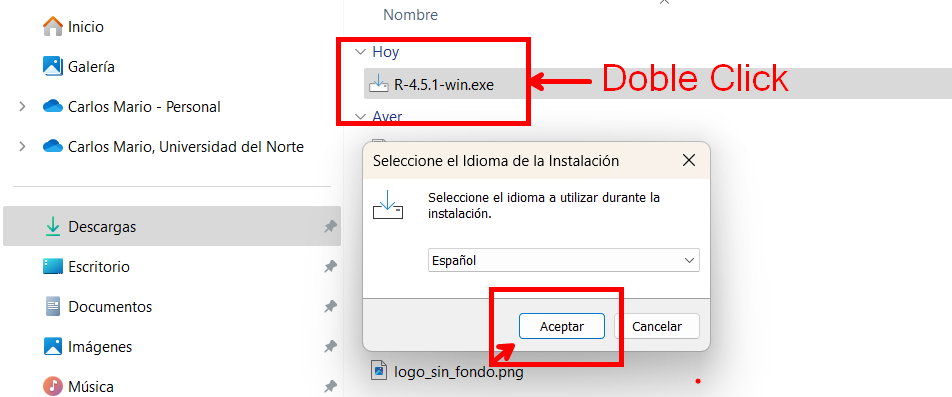
\includegraphics[width=0.48\linewidth]{images/r2} 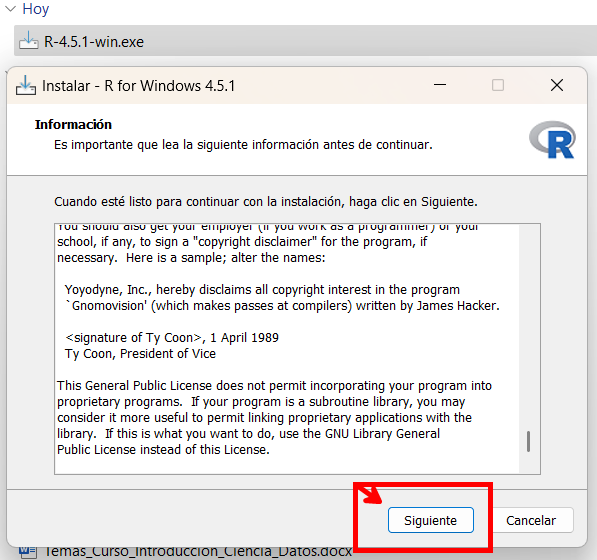
\includegraphics[width=0.48\linewidth]{images/r3} 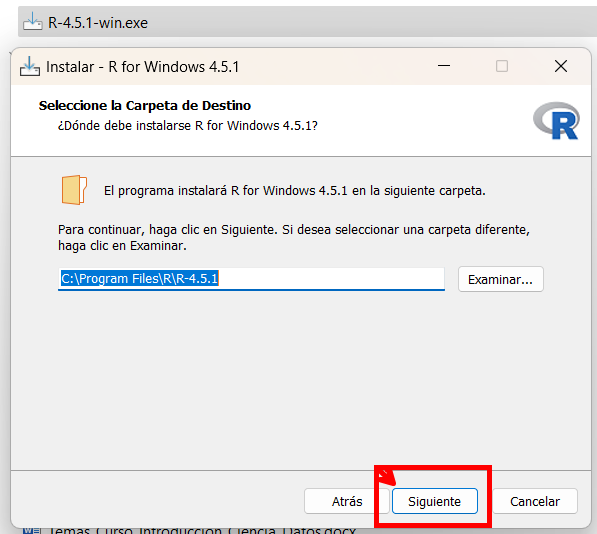
\includegraphics[width=0.48\linewidth]{images/r4} 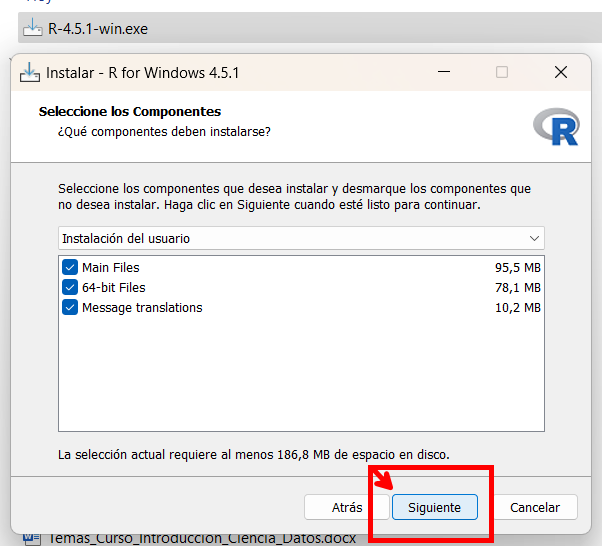
\includegraphics[width=0.48\linewidth]{images/r5} 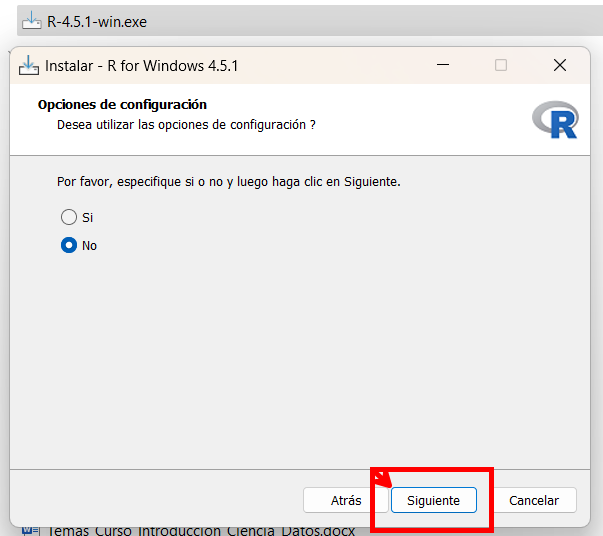
\includegraphics[width=0.48\linewidth]{images/r6} 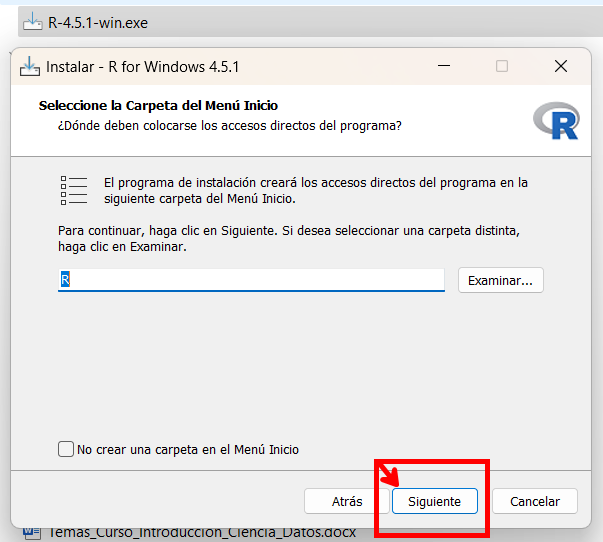
\includegraphics[width=0.48\linewidth]{images/r7} 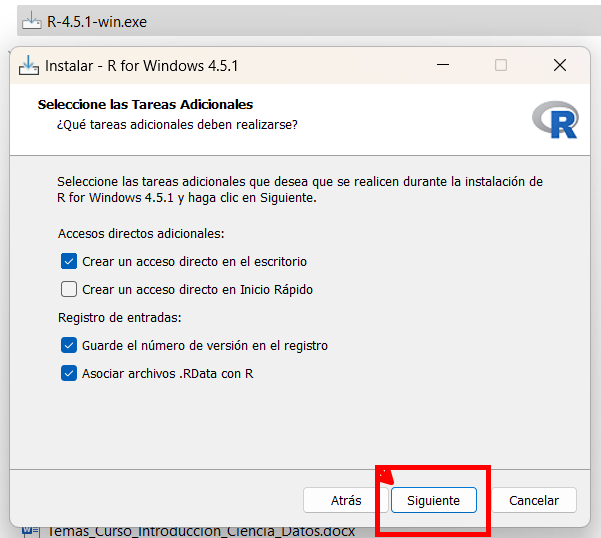
\includegraphics[width=0.48\linewidth]{images/r8} 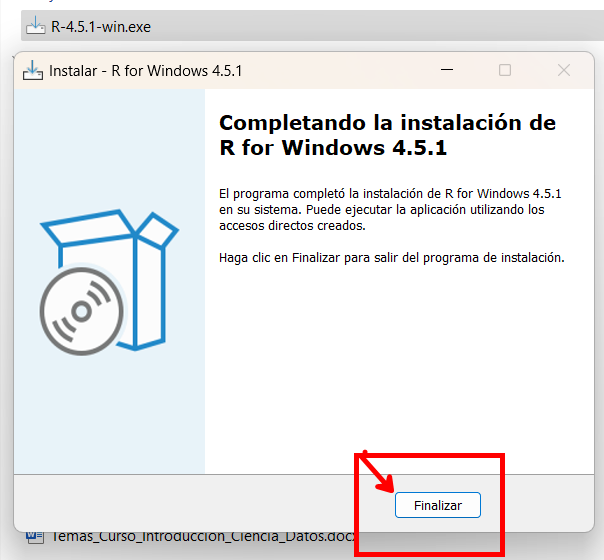
\includegraphics[width=0.48\linewidth]{images/r9} 

}

\caption{Paso a paso de la instalaci<U+00F3>n de R (izquierda a derecha)}\label{fig:inst-r-fig}
\end{figure}

\subsection{¿Qué es RStudio?}\label{quuxe9-es-rstudio}

\textbf{RStudio} es un \textbf{entorno de desarrollo integrado (IDE)} que proporciona una interfaz gráfica intuitiva y muy funcional para trabajar con R. Entre sus características destacan:

\begin{itemize}
\tightlist
\item
  Editor de scripts con \textbf{resaltado de sintaxis}.
\item
  Consola interactiva para ejecutar comandos.
\item
  Panel de visualización de datos y objetos en memoria.
\item
  Gráficos integrados.
\item
  Soporte para proyectos y versiones de R.
\item
  Integración con Git, Markdown, Quarto y Shiny.
\end{itemize}

Aunque se puede usar R sin RStudio, la mayoría de los usuarios prefieren trabajar dentro de este entorno por su productividad, organización y facilidad de uso.

A continuación, se indican los enlaces oficiales para descargar (paso a paso) \textbf{RStudio}:

\subsubsection*{Descargar RStudio}\label{descargar-rstudio}
\addcontentsline{toc}{subsubsection}{Descargar RStudio}

\begin{itemize}
\tightlist
\item
  Página oficial de RStudio (ahora llamado \textbf{Posit}, \url{https://posit.co/download/rstudio-desktop/}):
\end{itemize}

\begin{figure}

{\centering 
\includegraphics[width=0.3\linewidth]{images/rstudiosinfondo} 

}

\caption{Desarrollo de entorno integrado (IDE) RStudio}\label{fig:rs-fig}
\end{figure}

Selecciona la versión gratuita de \textbf{RStudio Desktop} y descarga el instalador correspondiente a tu sistema operativo.

Se realizará el proceso para la instalación de RStudio para el sistema operativo Windows:

\begin{figure}

{\centering 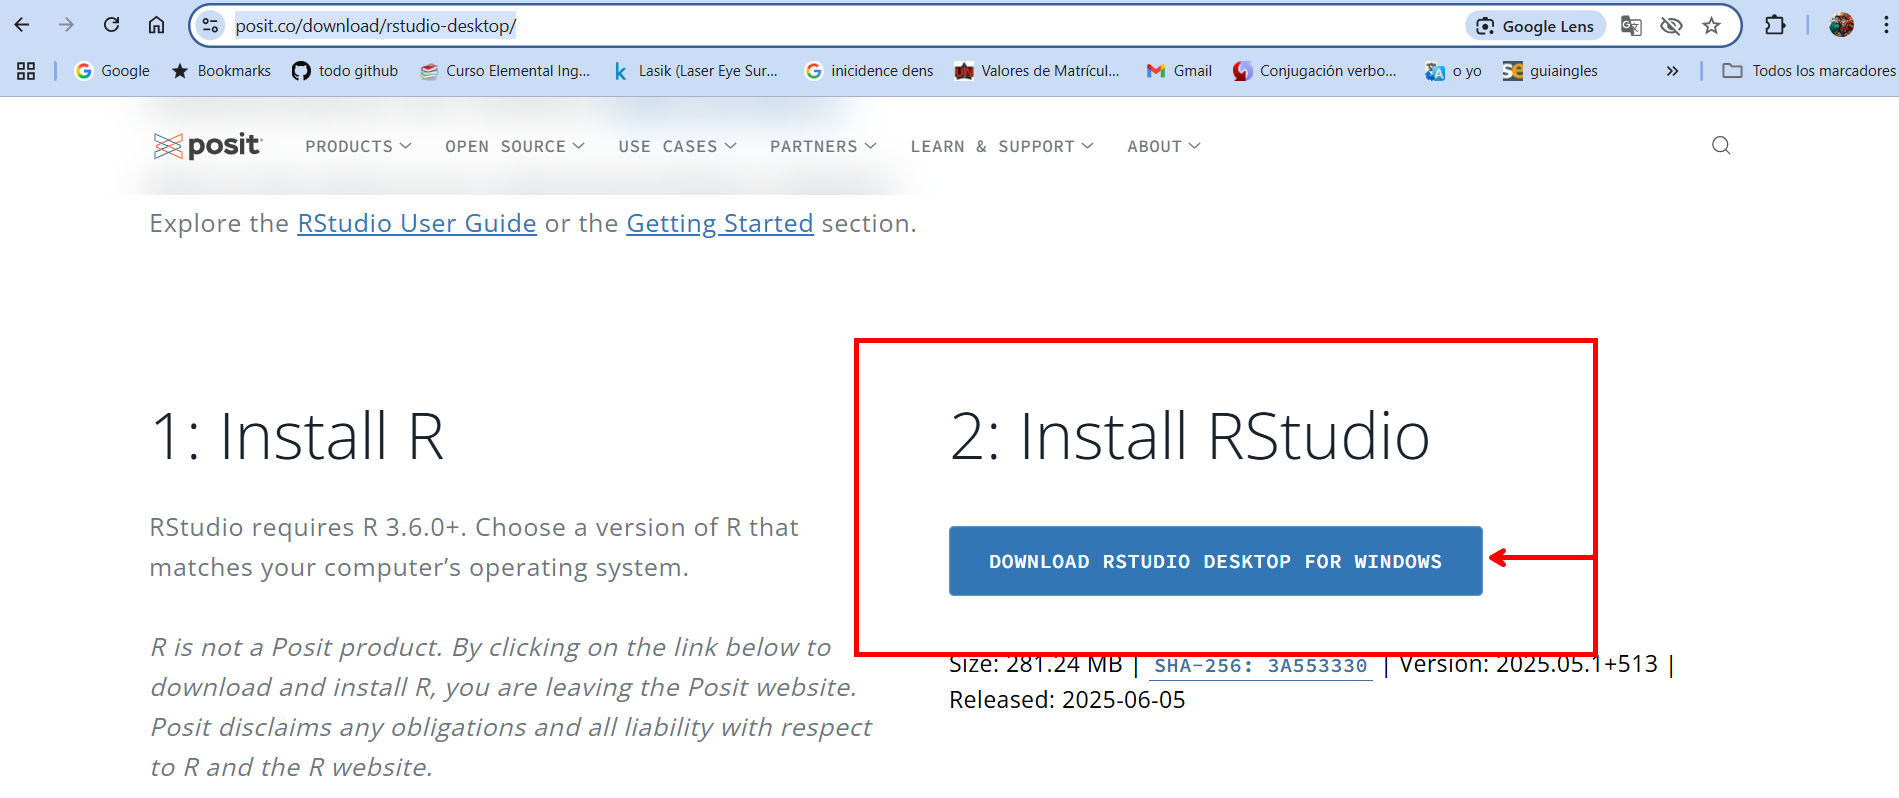
\includegraphics[width=0.48\linewidth]{images/rs1} 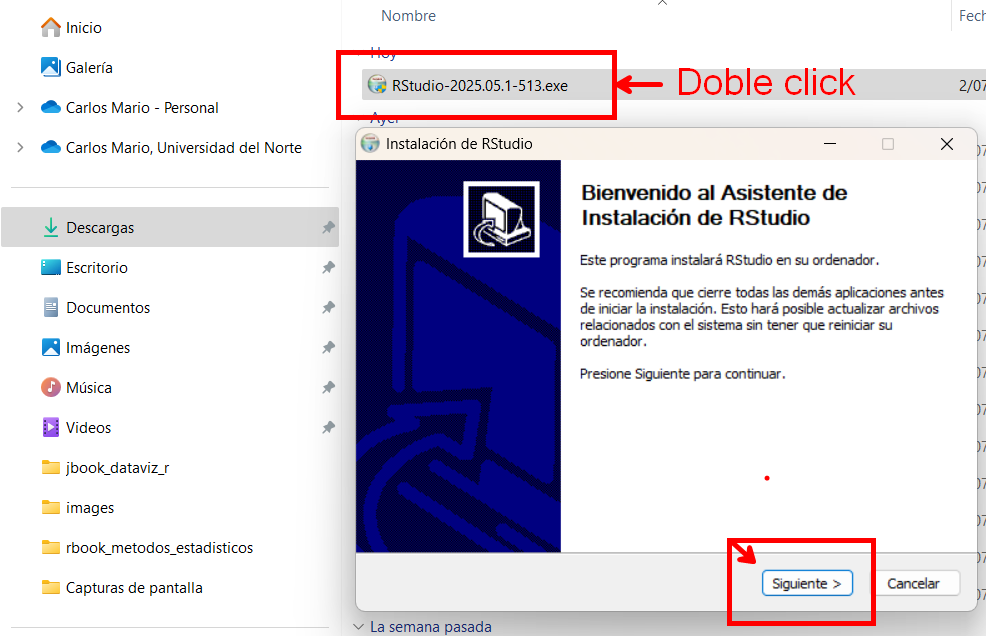
\includegraphics[width=0.48\linewidth]{images/rs2} 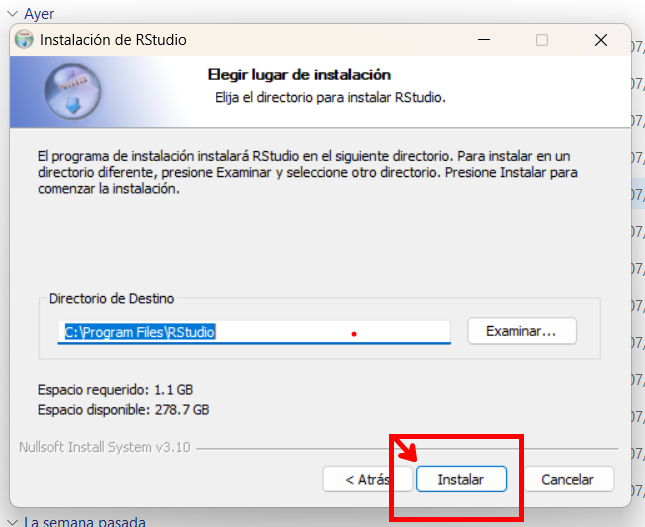
\includegraphics[width=0.48\linewidth]{images/rs3} 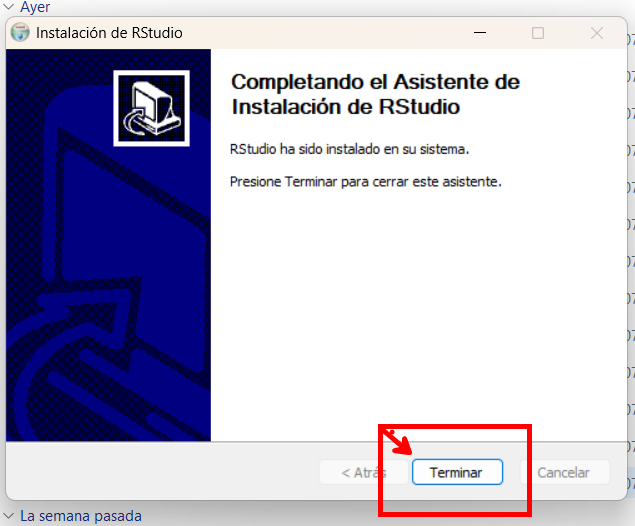
\includegraphics[width=0.48\linewidth]{images/rs4} 

}

\caption{Paso a paso de la instalaci<U+00F3>n de RStudio}\label{fig:inst-rs-fig}
\end{figure}

Una vez finalizada la instalación, puedes iniciar RStudio desde el acceso directo en tu escritorio o buscándolo en el menú de inicio.

\begin{figure}

{\centering 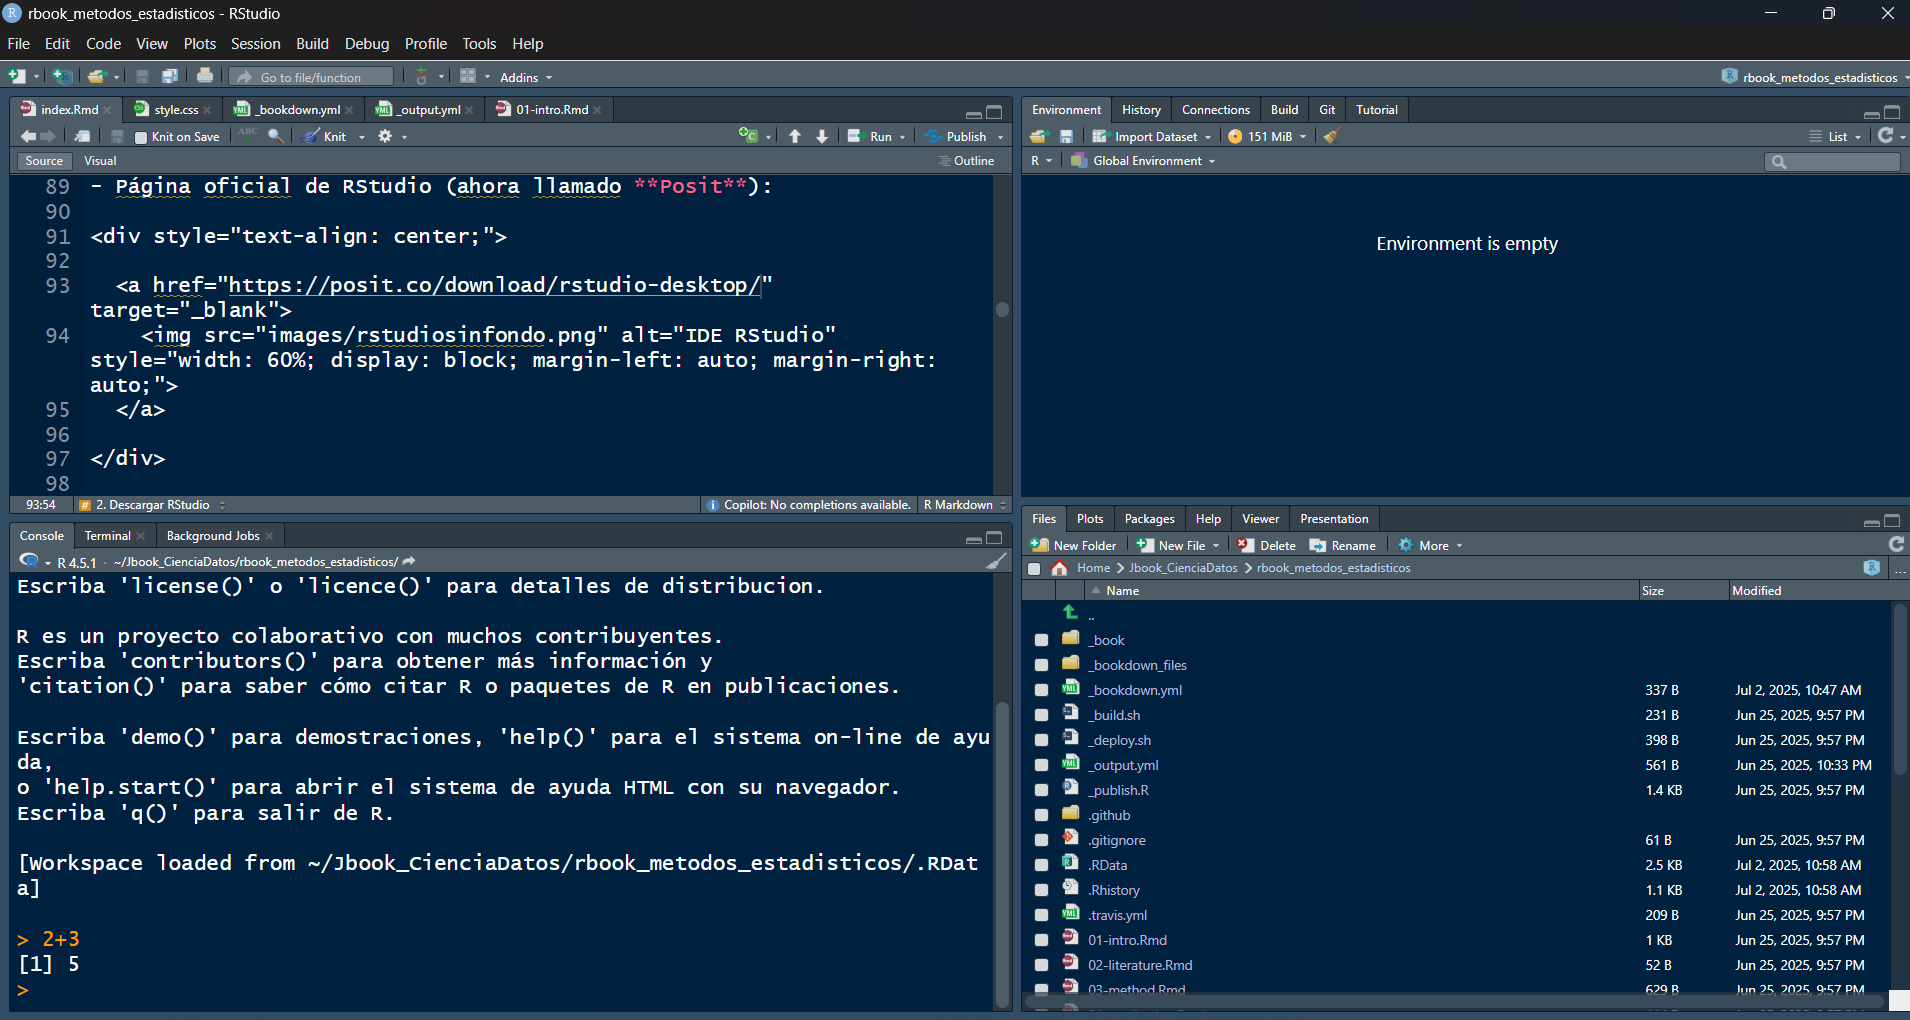
\includegraphics[width=1\linewidth]{images/rs5} 

}

\caption{Visualizaci<U+00F3>n de RStudio}\label{fig:rs-inst-fig}
\end{figure}

Al abrir RStudio por primera vez, se presenta un entorno dividido en cuatro paneles:

\begin{itemize}
\tightlist
\item
  \textbf{Script o editor de código} (arriba a la izquierda): donde se escriben los scripts \texttt{.R} o \texttt{.Rmd}.
\item
  \textbf{Consola} (abajo a la izquierda): donde se ejecutan los comandos directamente.
\item
  \textbf{Entorno / Historial} (arriba a la derecha): muestra los objetos cargados y el historial de comandos.
\item
  \textbf{Archivos, gráficos, paquetes, ayuda y visor} (abajo a la derecha): herramientas auxiliares para explorar y trabajar eficientemente.
\end{itemize}

Puedes verificar que R y RStudio están funcionando correctamente ejecutando una operación simple en la consola, como:

\begin{Shaded}
\begin{Highlighting}[]
\DecValTok{2} \SpecialCharTok{+} \DecValTok{3}
\end{Highlighting}
\end{Shaded}

\section{Introducción a Git y GitHub}\label{introducciuxf3n-a-git-y-github}

\subsection{¿Qué es Git?}\label{quuxe9-es-git}

\textbf{Git} es un sistema de control de versiones distribuido que permite gestionar y registrar los cambios realizados en archivos de un proyecto a lo largo del tiempo. Fue creado por Linus Torvalds y se ha convertido en el estándar para el desarrollo de software y proyectos colaborativos. El enlace es \url{https://git-scm.com/}.

\begin{figure}

{\centering 
\includegraphics[width=0.4\linewidth]{images/git} 

}

\caption{Sotfware Git}\label{fig:git-fig}
\end{figure}

{} Ventajas principales de Git

\begin{itemize}
\tightlist
\item
  Permite llevar un \textbf{historial detallado} de versiones.
\item
  Facilita la \textbf{colaboración} en proyectos con múltiples personas.
\item
  Permite trabajar en \textbf{ramas} (branches) para desarrollar funcionalidades de forma aislada.
\item
  No depende de internet para el trabajo local.
\end{itemize}

\subsubsection{Pasos para instalar Git}\label{pasos-para-instalar-git}

Daremos una guía para la instalación de \textbf{Git} usando Windows (paso a paso):

\begin{enumerate}
\def\labelenumi{\arabic{enumi}.}
\item
  Instalar \textbf{Git}:\\
  🔗 \url{https://git-scm.com/downloads}
\item
  Ahora, debes realizar lo siguiente:
\end{enumerate}

\begin{figure}

{\centering 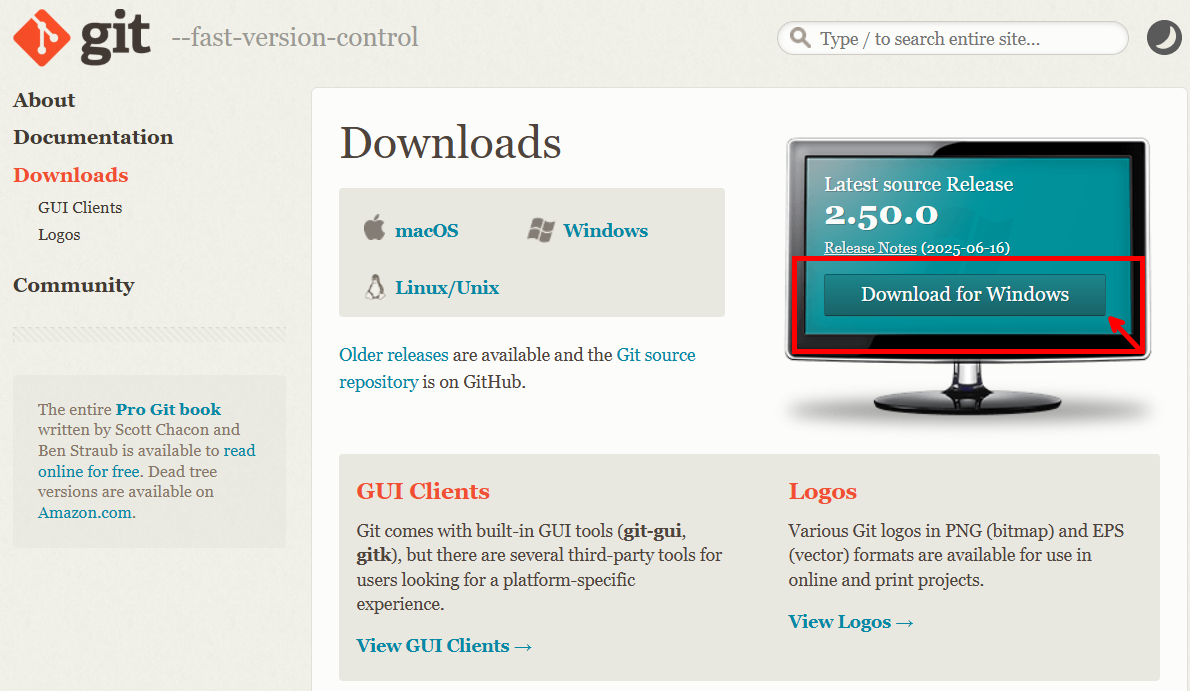
\includegraphics[width=0.48\linewidth]{images/git1} 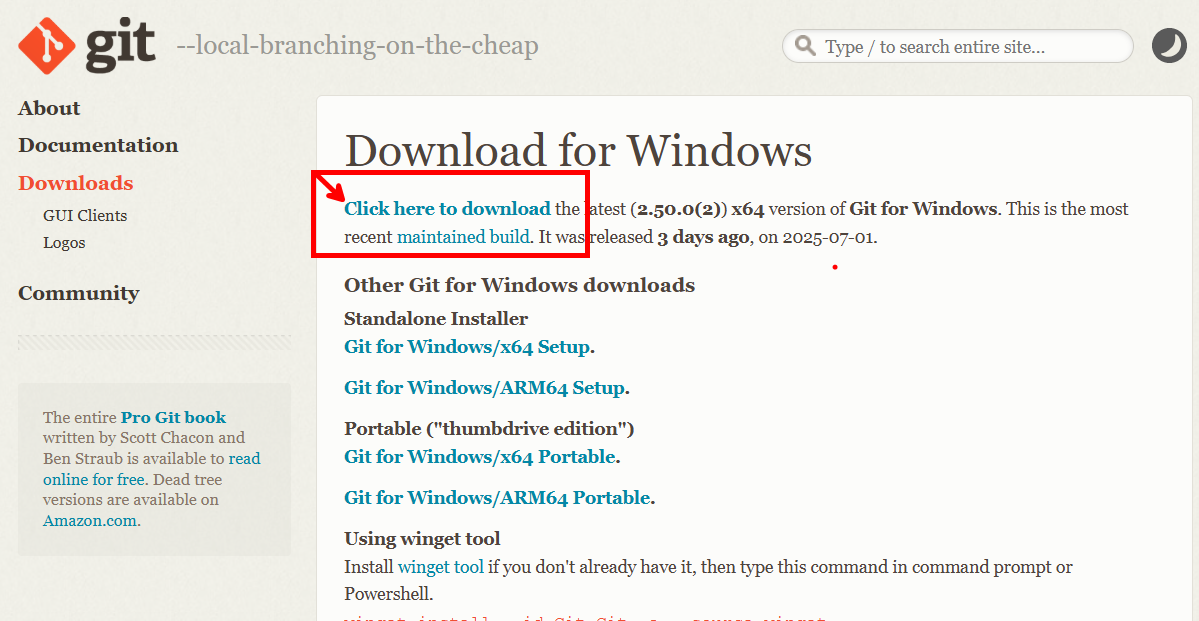
\includegraphics[width=0.48\linewidth]{images/git2} 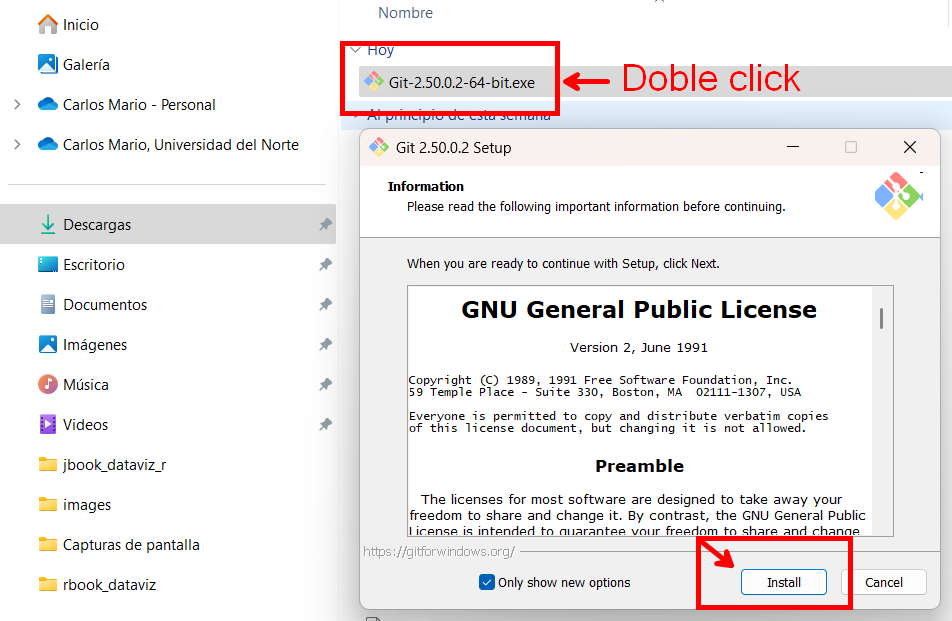
\includegraphics[width=0.48\linewidth]{images/git3} 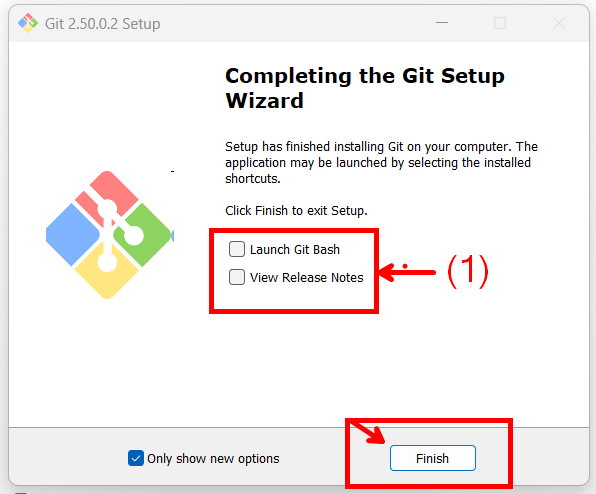
\includegraphics[width=0.48\linewidth]{images/git4} 

}

\caption{Instalaci<U+00F3>n de Git}\label{fig:git-inst-fig}
\end{figure}

\begin{enumerate}
\def\labelenumi{\arabic{enumi}.}
\setcounter{enumi}{2}
\tightlist
\item
  A continuación, comprobemos la instalación de Git.
\end{enumerate}

\begin{figure}

{\centering 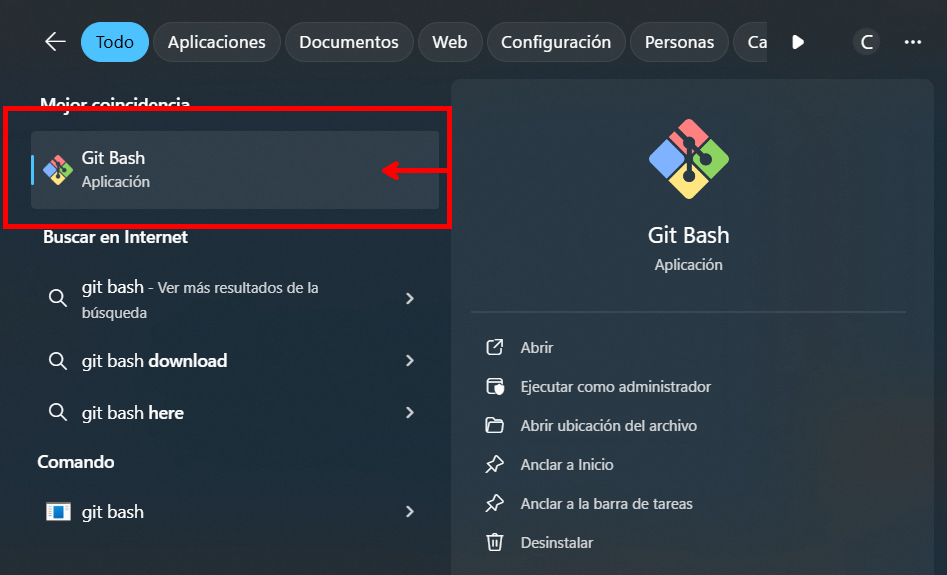
\includegraphics[width=0.48\linewidth]{images/gb1} 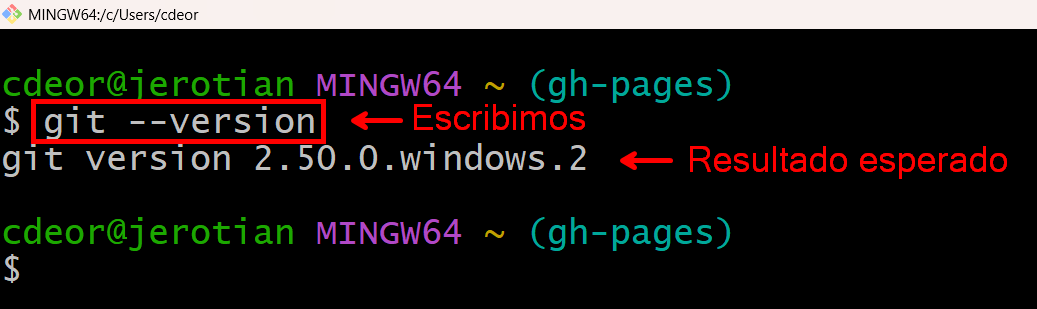
\includegraphics[width=0.48\linewidth]{images/gb2} 

}

\caption{Verificaci<U+00F3>n de Git}\label{fig:git-inst-b-fig}
\end{figure}

\subsection{¿Qué es GitHub?}\label{quuxe9-es-github}

\textbf{GitHub} es una plataforma en línea que permite alojar repositorios de Git en la nube. Es ideal para compartir proyectos, colaborar en equipo y automatizar flujos de trabajo. Este es el enlace \url{https://github.com}.

\begin{figure}

{\centering 
\includegraphics[width=0.3\linewidth]{images/github} 

}

\caption{Plataforma GitHub}\label{fig:github-fig}
\end{figure}

{} Funciones principales de GitHub

\begin{itemize}
\tightlist
\item
  Crear y administrar \textbf{repositorios} públicos o privados.
\item
  Gestionar cambios mediante \textbf{pull requests}.
\item
  Seguir errores o tareas usando \textbf{issues}.
\item
  Crear documentación, páginas web y wikis para los proyectos.
\item
  Automatizar procesos con \textbf{GitHub Actions}.
\end{itemize}

\subsubsection{Pasos para instalar GitHub}\label{pasos-para-instalar-github}

A continuación, se presenta una guía paso a paso para la instalación de \textbf{GitHub} en Windows:

\begin{enumerate}
\def\labelenumi{\arabic{enumi}.}
\item
  Crear una cuenta en \textbf{GitHub}:\\
  🔗 \url{https://github.com}
\item
  Ahora, sigue las imagenes:
\end{enumerate}

\begin{figure}

{\centering 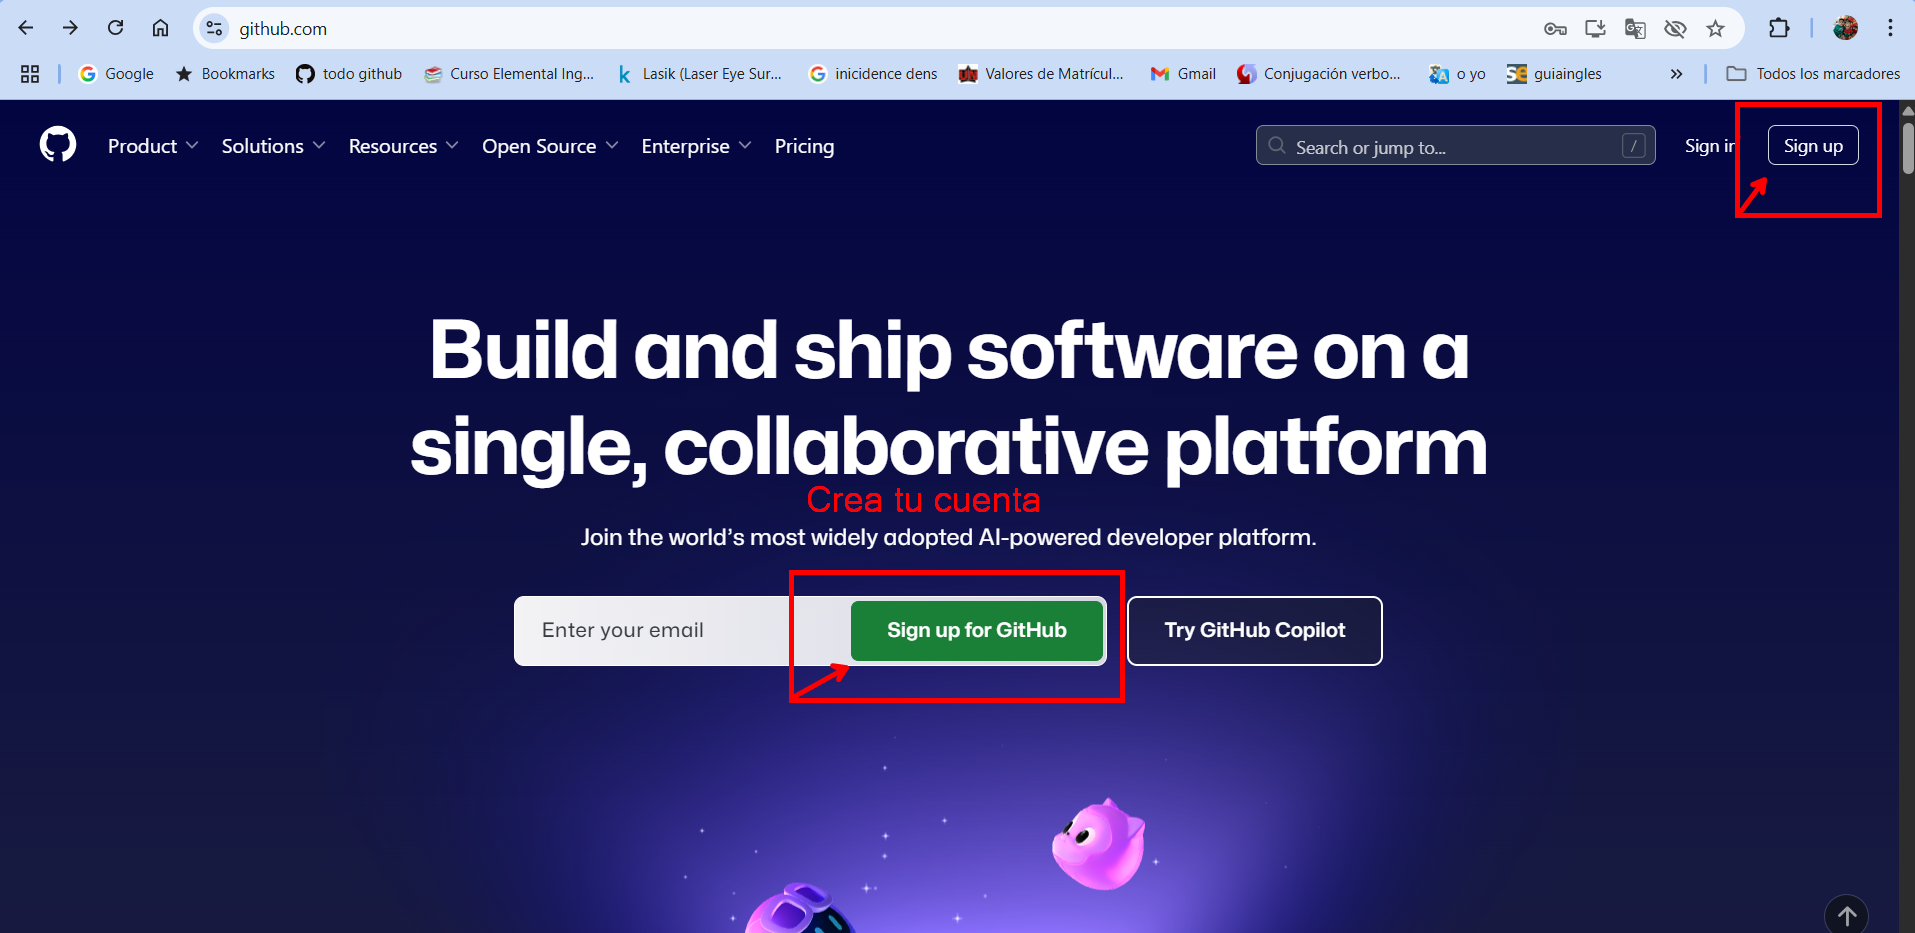
\includegraphics[width=0.8\linewidth]{images/gh1} 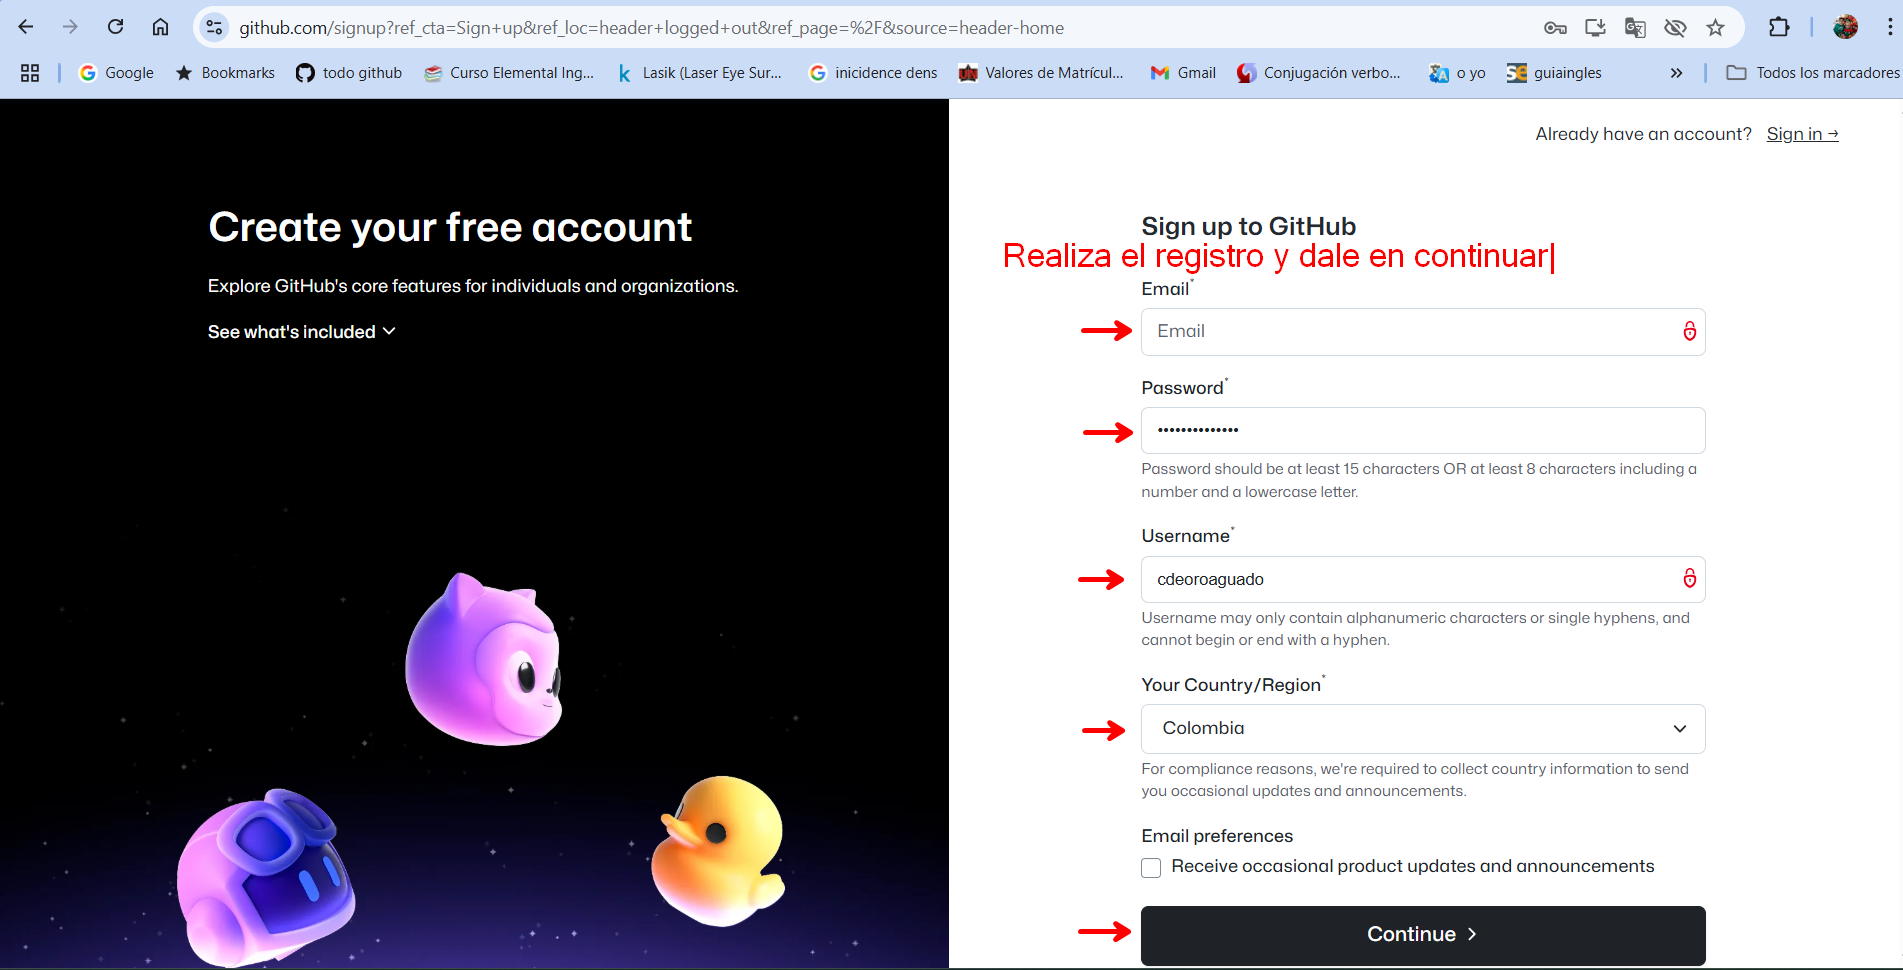
\includegraphics[width=0.8\linewidth]{images/gh2} 

}

\caption{Registro en GitHub}\label{fig:github-b-fig}
\end{figure}

Despues haces el proceso de verificación

\begin{itemize}
\item
  Completa el captcha de seguridad.
\item
  GitHub puede pedirte que verifiques tu correo electrónico. Revisa tu bandeja de entrada y haz clic en el enlace de confirmación.
\end{itemize}

\begin{enumerate}
\def\labelenumi{\arabic{enumi}.}
\setcounter{enumi}{2}
\tightlist
\item
  Ingresas al enlace \url{https://github.com} y despues:
\end{enumerate}

\begin{figure}

{\centering 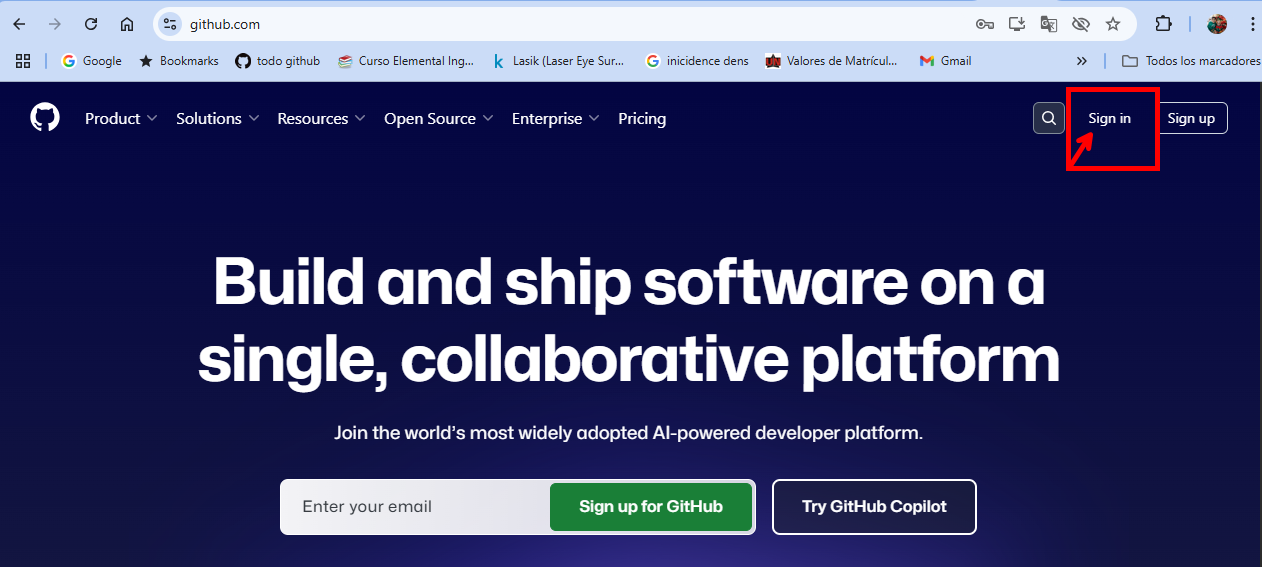
\includegraphics[width=0.7\linewidth]{images/gh3} 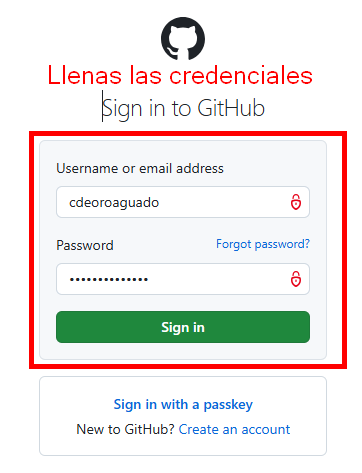
\includegraphics[width=0.7\linewidth]{images/gh4} 

}

\caption{Credenciales de verificaci<U+00F3>n en GitHub}\label{fig:github-c-fig}
\end{figure}

Al ingresar, este sería el inicio

\begin{figure}

{\centering 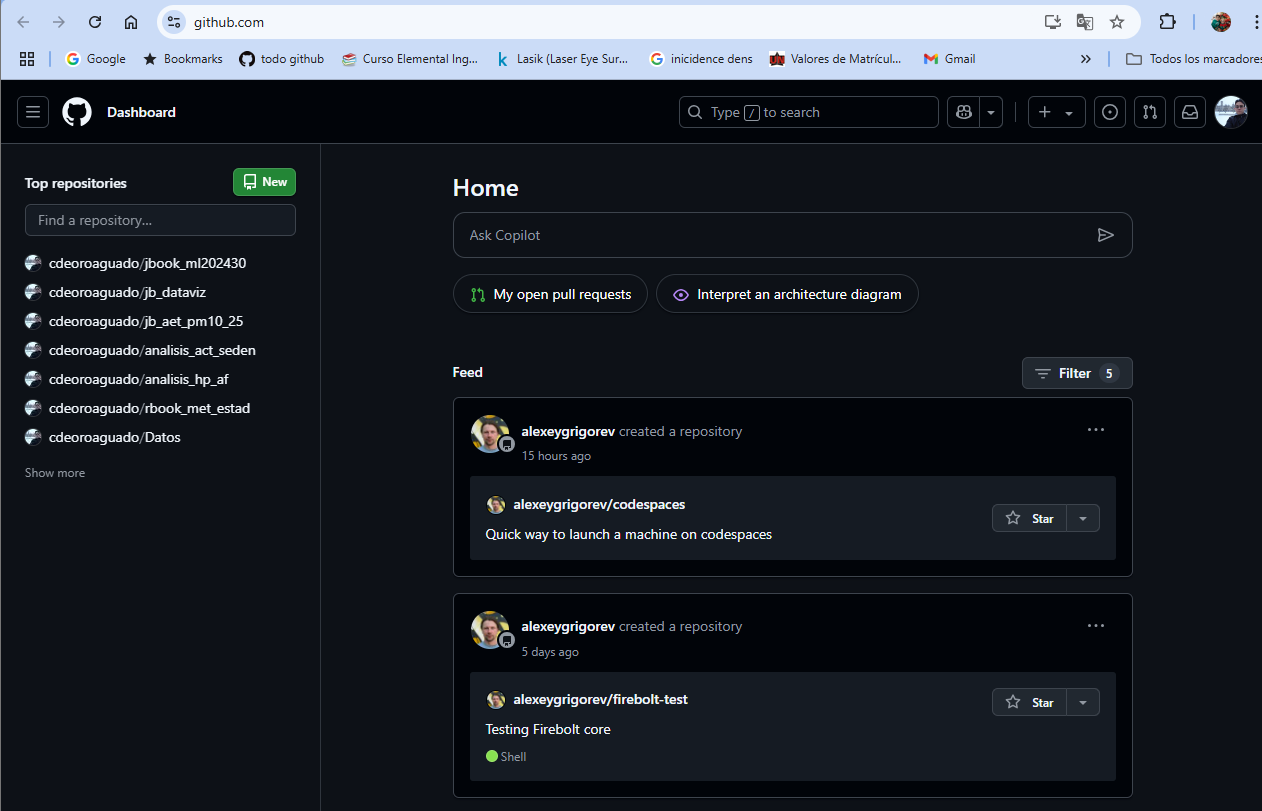
\includegraphics[width=1\linewidth]{images/gh5} 

}

\caption{Dashboard de GitHub}\label{fig:github-d-fig}
\end{figure}

\begin{enumerate}
\def\labelenumi{\arabic{enumi}.}
\setcounter{enumi}{3}
\tightlist
\item
  A continuación, vamos a descargar \textbf{GitHub Desktop} para Windows; para ello debes usar el enlace \url{https://desktop.github.com/download/}
\end{enumerate}

\begin{figure}

{\centering 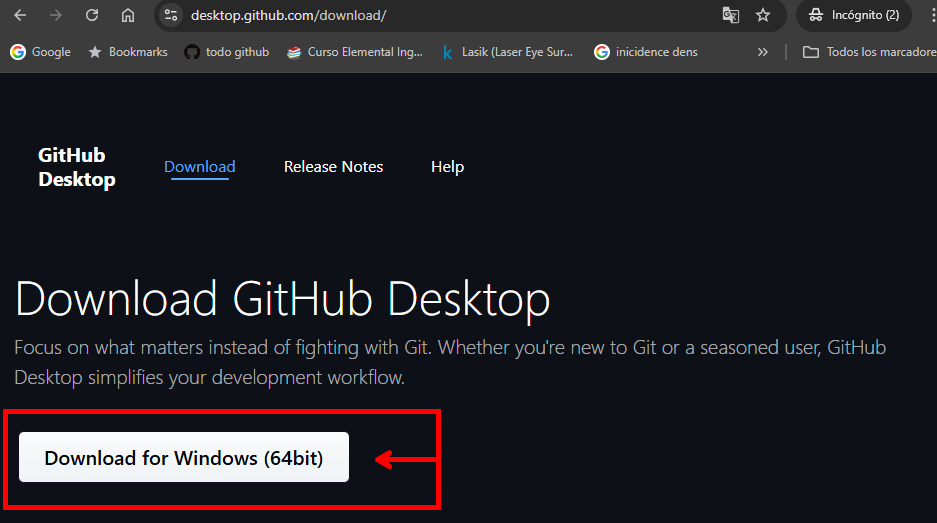
\includegraphics[width=0.48\linewidth]{images/ghd1} 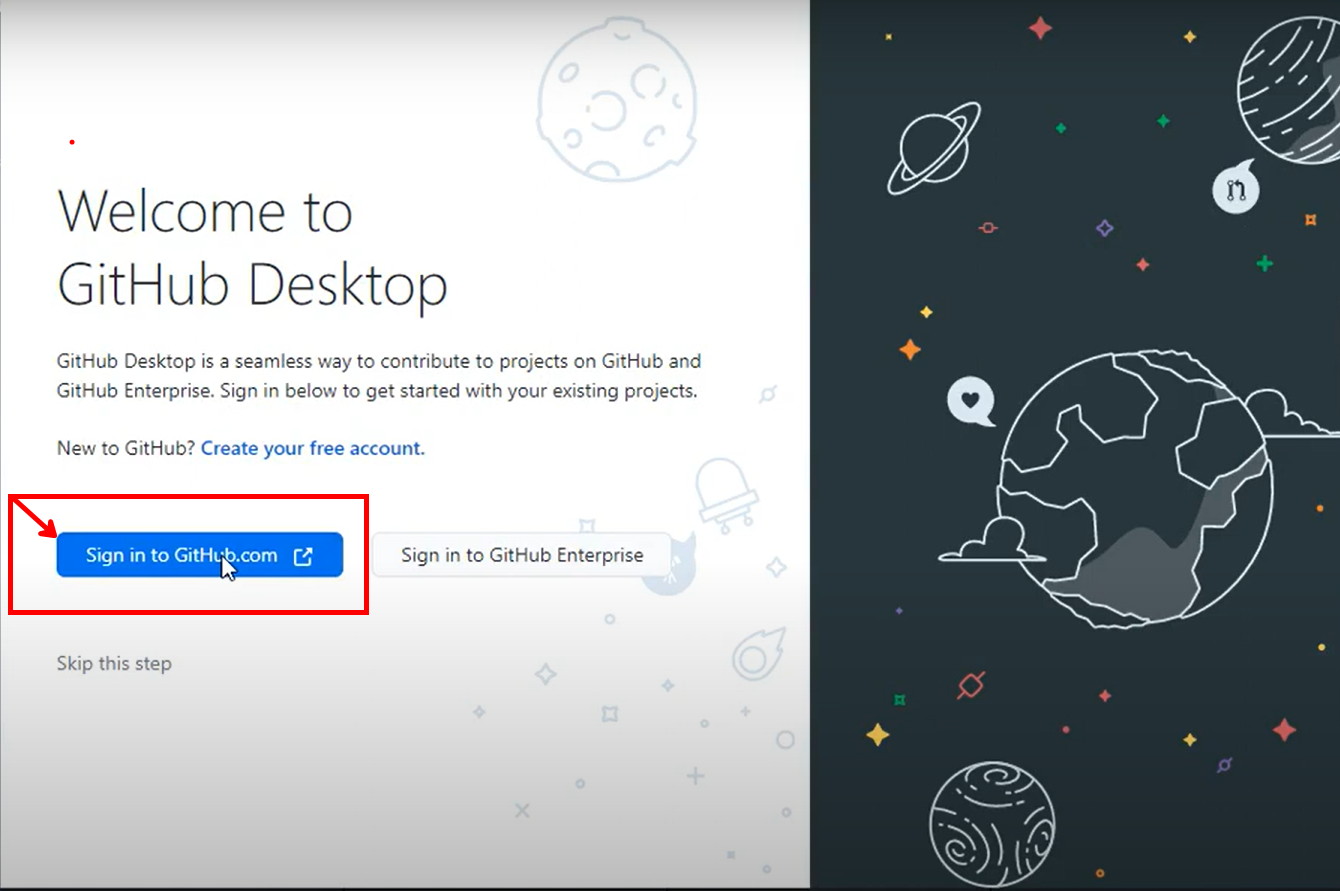
\includegraphics[width=0.48\linewidth]{images/ghd2} 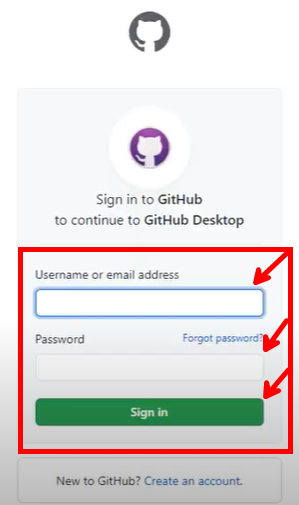
\includegraphics[width=0.48\linewidth]{images/ghd3} 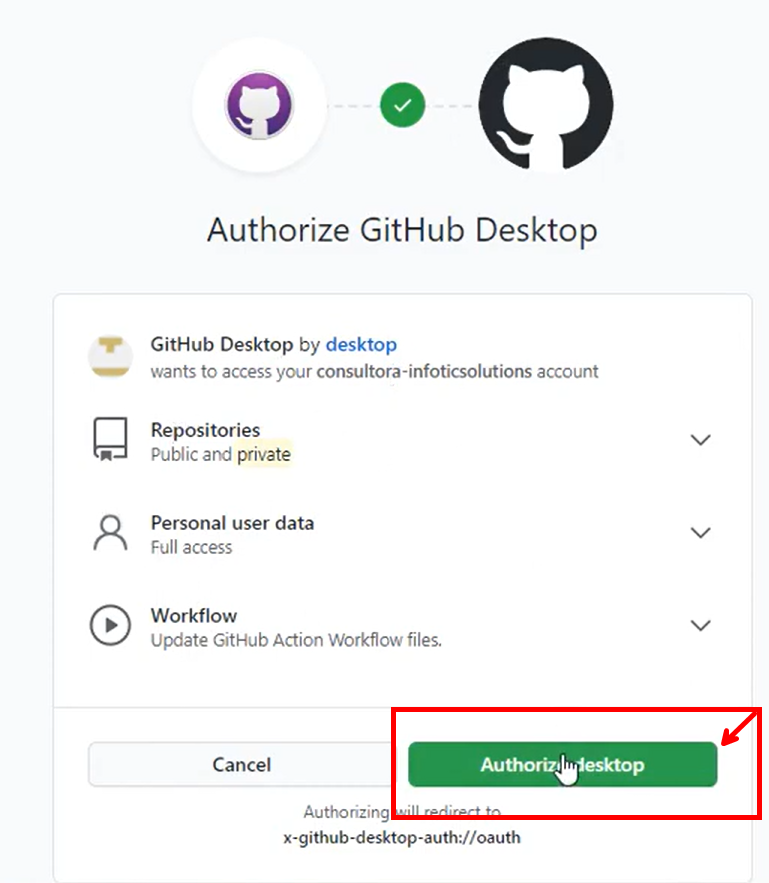
\includegraphics[width=0.48\linewidth]{images/ghd4} 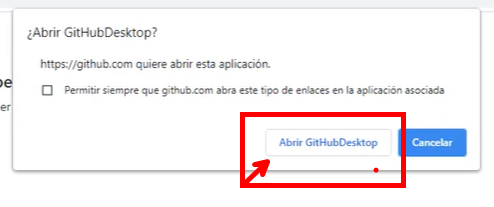
\includegraphics[width=0.48\linewidth]{images/ghd5} 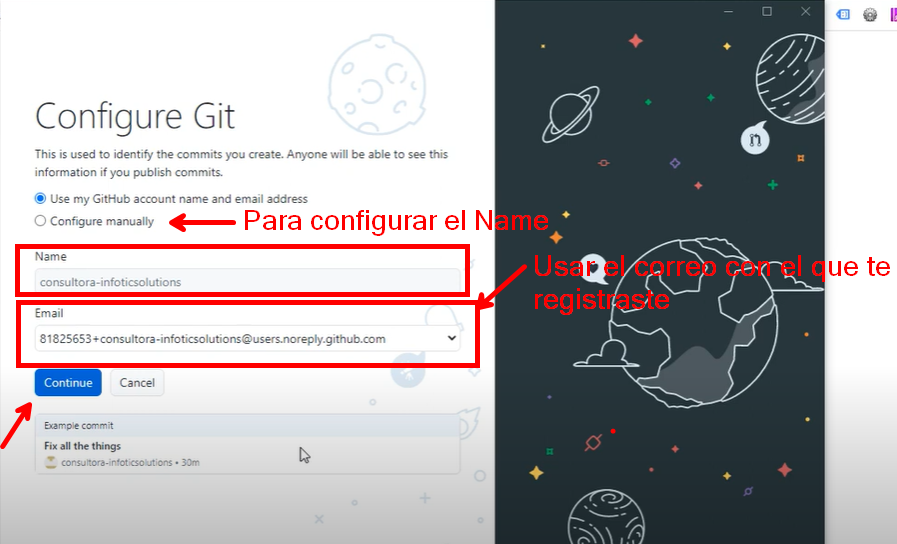
\includegraphics[width=0.48\linewidth]{images/ghd6} 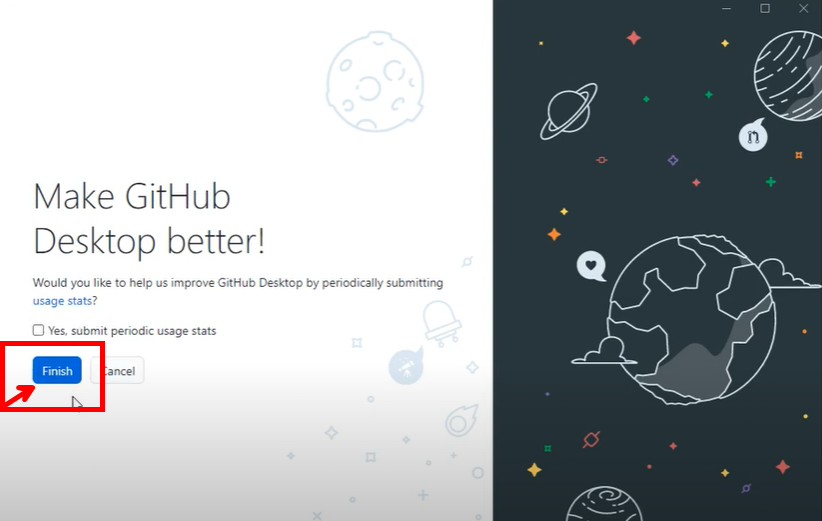
\includegraphics[width=0.48\linewidth]{images/ghd7} 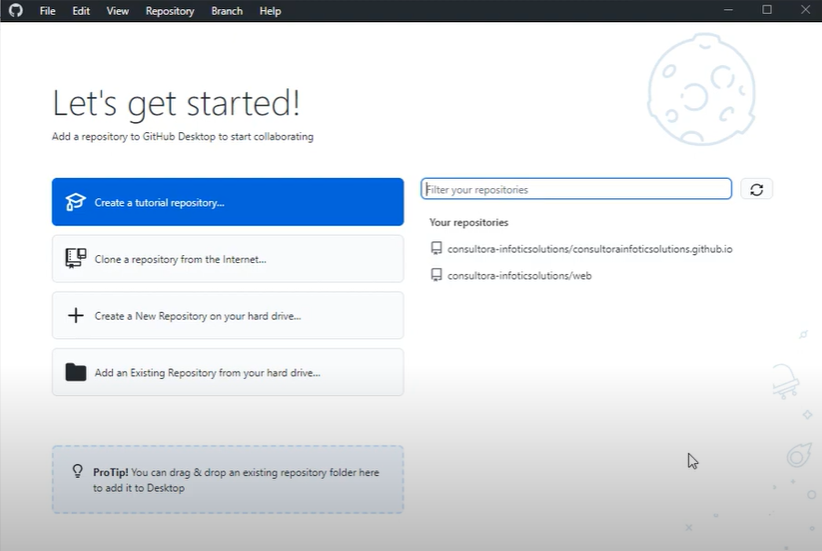
\includegraphics[width=0.48\linewidth]{images/ghd8} 

}

\caption{Credenciales de verificaci<U+00F3>n en GitHub}\label{fig:github-e-fig}
\end{figure}

\subsubsection*{Diferencias claves entre Git y GitHub}\label{diferencias-claves-entre-git-y-github}
\addcontentsline{toc}{subsubsection}{Diferencias claves entre Git y GitHub}

\begin{longtable}[]{@{}ll@{}}
\toprule\noalign{}
Git & GitHub \\
\midrule\noalign{}
\endhead
\bottomrule\noalign{}
\endlastfoot
Herramienta local & Plataforma en la nube \\
Administra versiones & Aloja y comparte repositorios \\
No requiere internet & Requiere conexión para sincronizar \\
Se usa desde terminal o IDE & Se accede por navegador o API \\
\end{longtable}

\subsubsection{¿Cómo se relacionan?}\label{cuxf3mo-se-relacionan}

\begin{itemize}
\tightlist
\item
  Git administra tu proyecto \textbf{localmente}, guardando versiones y cambios.
\item
  GitHub actúa como \textbf{repositorio remoto}, permitiendo subir (\texttt{push}) o descargar (\texttt{pull}) cambios desde y hacia otros colaboradores.
\item
  Juntos permiten trabajar de forma segura, organizada y colaborativa desde distintos lugares.
\end{itemize}

\section{\texorpdfstring{Pasos para publicar un libro \texttt{bookdown} en GitHub Pages}{Pasos para publicar un libro bookdown en GitHub Pages}}\label{pasos-para-publicar-un-libro-bookdown-en-github-pages}

Para publicar un libro bookdown en GitHub Pages debes tener lo siguiente:

\begin{enumerate}
\def\labelenumi{\arabic{enumi}.}
\tightlist
\item
  Pre-requisitos
\end{enumerate}

\begin{itemize}
\item
  Tener una cuenta en GitHub.
\item
  Haber creado un repositorio público (ej. metodos\_estadisticos).
\item
  Tener Git instalado y configurado.
\item
  Tener \texttt{R} y \texttt{RStudio} instalado y configurado
\item
  Instalar el siguiente paquete
\end{itemize}

\begin{Shaded}
\begin{Highlighting}[]
\FunctionTok{install.packages}\NormalTok{(}\StringTok{"bookdown"}\NormalTok{)}
\end{Highlighting}
\end{Shaded}

\begin{itemize}
\tightlist
\item
  Tener un proyecto bookdown funcional en tu computadora.
\end{itemize}

\begin{enumerate}
\def\labelenumi{\arabic{enumi}.}
\setcounter{enumi}{1}
\tightlist
\item
  Abre el archivo \texttt{\_bookdown.yml} y asegúrate de incluir:
\end{enumerate}

\begin{Shaded}
\begin{Highlighting}[]
\FunctionTok{book\_filename}\KeywordTok{:}\AttributeTok{ }\StringTok{"index"}
\FunctionTok{output\_dir}\KeywordTok{:}\AttributeTok{ }\StringTok{"docs"}
\end{Highlighting}
\end{Shaded}

Esto hace que el libro se renderice en la carpeta docs, que es donde GitHub Pages busca el sitio por defecto.

\begin{enumerate}
\def\labelenumi{\arabic{enumi}.}
\setcounter{enumi}{2}
\tightlist
\item
  En RStudio o consola de R, corre:
\end{enumerate}

\begin{Shaded}
\begin{Highlighting}[]
\NormalTok{bookdown}\SpecialCharTok{::}\FunctionTok{render\_book}\NormalTok{(}\StringTok{"index.Rmd"}\NormalTok{)}
\end{Highlighting}
\end{Shaded}

\begin{enumerate}
\def\labelenumi{\arabic{enumi}.}
\setcounter{enumi}{3}
\tightlist
\item
  Abre la terminal en la carpeta del libro y ejecuta:
\end{enumerate}

\begin{Shaded}
\begin{Highlighting}[]
\FunctionTok{git}\NormalTok{ init}
\FunctionTok{git}\NormalTok{ remote add origin https://github.com/cdeoroaguado/rbook\_dataviz.git}
\FunctionTok{git}\NormalTok{ add docs}
\FunctionTok{git}\NormalTok{ commit }\AttributeTok{{-}m} \StringTok{"primer despliegue del libro"}
\FunctionTok{git}\NormalTok{ push }\AttributeTok{{-}u}\NormalTok{ origin main }
\end{Highlighting}
\end{Shaded}

\begin{enumerate}
\def\labelenumi{\arabic{enumi}.}
\setcounter{enumi}{4}
\tightlist
\item
  Activa GitHub Pages
\end{enumerate}

\begin{itemize}
\item
  Ve al repositorio en GitHub.
\item
  Haz clic en \texttt{Settings\ \textgreater{}\ Pages}.
\item
  En ``Source'', selecciona:

  \begin{itemize}
  \tightlist
  \item
    \texttt{Branch:\ main\ o\ master}
  \item
    \texttt{Folder:\ /docs}
  \end{itemize}
\item
  Guarda los cambios.
\end{itemize}

\begin{enumerate}
\def\labelenumi{\arabic{enumi}.}
\setcounter{enumi}{5}
\tightlist
\item
  Después de unos segundos, tu libro estará disponible en:
\end{enumerate}

{} Enlace del texto

Dale click en este enlace:

👉 \url{https://cdeoroaguado.github.io/rbook_dataviz/}

\subsection{Video paso a paso de la publicación del libro en GitHub Pages}\label{video-paso-a-paso-de-la-publicaciuxf3n-del-libro-en-github-pages}

Uno de los pasos más importantes al desarrollar un libro con \texttt{bookdown} es su publicación en línea, permitiendo el acceso abierto y permanente al contenido. Para ello, \texttt{GitHub\ Pages} se convierte en una herramienta ideal por su facilidad de uso y compatibilidad con proyectos de R. A continuación, se presenta un video tutorial donde se explican paso a paso los procedimientos necesarios para publicar correctamente un libro elaborado en \texttt{bookdown} a través de un repositorio en GitHub:

Cabe resaltar que este libro de muestra estamos utilizando el paquete bookdown \citep{R-bookdown}, el cual fue construido sobre R Markdown y knitr \citep{xie2015}

\chapter{ETL con Tidyverse}\label{etltidyverse}

El \textbf{Tidyverse} es un conjunto de paquetes integrados para el lenguaje de programación R, diseñados con el objetivo de facilitar el análisis de datos de manera estructurada, legible y eficiente. Su filosofía se basa en el concepto de \textbf{``datos ordenados'' (tidy data)}, donde cada variable es una columna, cada observación una fila, y cada tipo de unidad observacional forma una tabla.

Estos paquetes comparten principios de diseño comunes y una gramática coherente, lo que permite a los usuarios aprender un conjunto de reglas aplicables en todo el ecosistema, aumentando así la productividad y la claridad del código.

\begin{figure}

{\centering 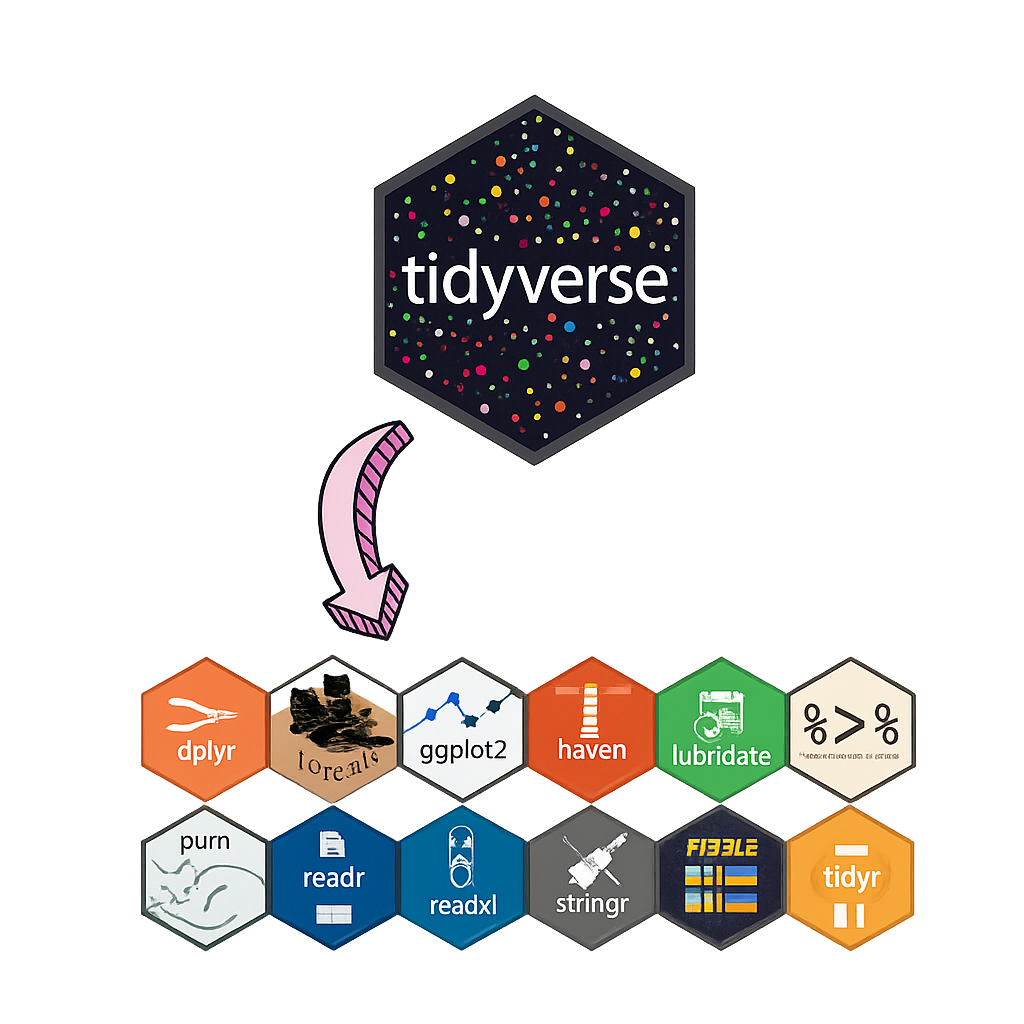
\includegraphics[width=0.7\linewidth]{images/tidypacsinfondo} 

}

\caption{Paquetes de tidyverse}\label{fig:tidy-fig}
\end{figure}

\section{Data Frames}\label{data-frames}

{} Definición

Un data frame es una estructura de datos clave en estadística y en R.

\begin{itemize}
\tightlist
\item
  La estructura básica de un data frame es que \emph{hay una observación por fila y cada columna representa una variable, medida, rasgo o característica de esa observación}.\\
\item
  \textbf{R} tiene una implementación interna de los data frames que probablemente es la que más se utiliza en la práctica.
\end{itemize}

\section{Importación de datos}\label{importaciuxf3n-de-datos}

{} Fuentes de datos en R

Los conjuntos de datos de gran tamaño, generalmente almacenados como data frames en R, suelen provenir de archivos externos.\\
Existen múltiples tipos de archivos que pueden importarse, entre ellos:\\

Archivos de texto en formatos como csv, txt, html y json.

Salidas de software estadístico como SAS y SPSS.

Recursos en línea como páginas html y servicios web.

Bases de datos relacionales y no relacionales.

El ecosistema Tidyverse ofrece funciones que permiten importar y gestionar estas diversas fuentes de datos de manera sencilla y eficiente.

\subsection{\texorpdfstring{Importación de archivos \texttt{csv} con \texttt{read.table()}}{Importación de archivos csv con read.table()}}\label{importaciuxf3n-de-archivos-csv-con-read.table}

{} Definición

La función read.table() es una función integrada en R que permite leer archivos de distintos formatos y convertirlos en un data frame.\\
Es una de las funciones más utilizadas para importar archivos simples en R.

La sintaxis de \textbf{\texttt{read.table()}} requiere indicar:\\
- Un nombre de archivo (ruta de acceso).\\
- Un valor lógico (\textbf{\texttt{TRUE/FALSE}}) para definir si la primera fila contiene los nombres de las columnas.

\begin{itemize}
\tightlist
\item
  Si se establece en \textbf{\texttt{TRUE}}, la primera fila se interpreta como encabezado.\\
\item
  Si se establece en \textbf{\texttt{FALSE}}, las columnas se importan sin nombres definidos.
\end{itemize}

El resultado de la función siempre es un \textbf{data frame}.

Una alternativa práctica es la función \textbf{\texttt{file.choose()}}, que permite seleccionar el archivo de manera interactiva sin necesidad de escribir la ruta manualmente.

{} Observación

Pasos para importar un archivo \texttt{csv} con read.table():

Abrir RStudio y dirigirse a la consola.

Establecer el directorio de trabajo con código en la consola o desde el menú:
Sesión → Establecer directorio de trabajo → Elegir directorio.

Ejecutar la función read.table() indicando el archivo \texttt{csv} a importar.

\begin{Shaded}
\begin{Highlighting}[]
\FunctionTok{setwd}\NormalTok{(}\StringTok{"\textasciitilde{}/Books\_CienciaDatos/rbook\_dataviz"}\NormalTok{)}
\end{Highlighting}
\end{Shaded}

\begin{figure}

{\centering 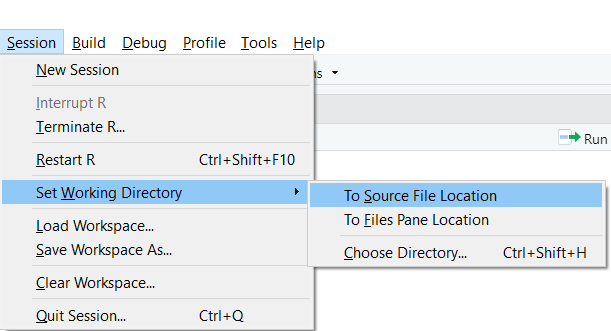
\includegraphics[width=0.7\linewidth]{images/setwd} 

}

\caption{setwd}\label{fig:fig-2}
\end{figure}

\begin{itemize}
\item
  En la carpeta \textbf{\href{https://github.com/cdeoroaguado/Datos/blob/main/datarstudio/RDataSets.zip}{RDataSets}} se encuentra el archivo \textbf{StudyArea.csv}, que corresponde a un archivo separado por comas.\\
  Este archivo contiene información sobre incendios forestales ocurridos entre los años 1980 y 2016 en distintos estados de EE. UU., entre ellos: California, Oregón, Washington, Idaho, Montana, Wyoming, Colorado, Utah, Nevada, Arizona y Nuevo México.
\item
  El archivo incluye más de \textbf{439000 registros} distribuidos en \textbf{37 columnas}, que describen las características de cada incendio durante ese periodo.
\item
  Para cargar estos datos en un nuevo objeto \textbf{data frame}, puede utilizarse la función \texttt{read.table()} de la siguiente manera:
\end{itemize}

\begin{Shaded}
\begin{Highlighting}[]
\NormalTok{df }\OtherTok{\textless{}{-}} \FunctionTok{read.table}\NormalTok{(}\StringTok{"data/StudyArea.csv"}\NormalTok{, }\AttributeTok{header =} \ConstantTok{TRUE}\NormalTok{)}
\end{Highlighting}
\end{Shaded}

\begin{itemize}
\tightlist
\item
  Recibirá un mensaje de error cuando intente ejecutar esta línea de código. El mensaje de error mensaje de error debería aparecer como se ve a continuación
\end{itemize}

\begin{figure}

{\centering 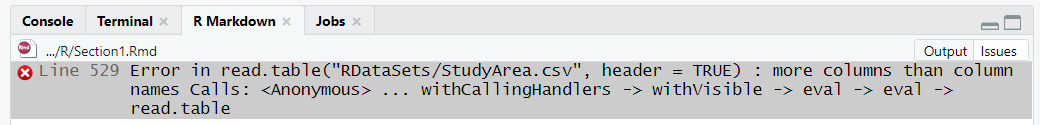
\includegraphics[width=0.7\linewidth]{images/error} 

}

\caption{error en rmd}\label{fig:fig-3}
\end{figure}

\begin{itemize}
\tightlist
\item
  La razón por la que se generó un mensaje de error en este caso es que la función \textbf{\texttt{read.table()}} utiliza espacios como delimitador entre registros y nuestro archivo utiliza comas como delimitador
\end{itemize}

Actualice su llamada a \textbf{\texttt{read.table()}} como se ve a continuación para incluir el argumento \textbf{\texttt{sep}}, que debería ser una coma

\begin{Shaded}
\begin{Highlighting}[]
\NormalTok{df }\OtherTok{\textless{}{-}} \FunctionTok{read.table}\NormalTok{(}\StringTok{"data/StudyArea.csv"}\NormalTok{, }\AttributeTok{sep=}\StringTok{","}\NormalTok{, }\AttributeTok{header =} \ConstantTok{TRUE}\NormalTok{)}
\end{Highlighting}
\end{Shaded}

\begin{itemize}
\tightlist
\item
  Cuando ejecute esta línea de código verá un nuevo error
\end{itemize}

\begin{figure}

{\centering 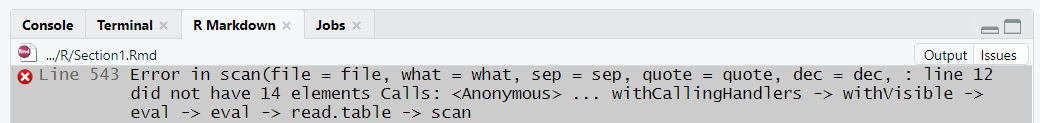
\includegraphics[width=0.75\linewidth]{images/error2} 

}

\caption{continuaci<U+00F3>n del error en rmd}\label{fig:fig-4}
\end{figure}

\begin{itemize}
\tightlist
\item
  La función \texttt{read.table()} no completa de manera automática las celdas vacías con un valor por defecto como \texttt{NA}.\\
  Por este motivo, si alguna fila del archivo no contiene el número esperado de columnas (en este caso, 14), se genera un mensaje de error durante la importación.
\end{itemize}

Para solucionar este inconveniente, puede añadirse el parámetro \texttt{fill\ =\ TRUE}, lo que permite a \textbf{R} rellenar los espacios vacíos con \texttt{NA} y mantener la estructura correcta del \texttt{data.frame}.

\begin{Shaded}
\begin{Highlighting}[]
\NormalTok{df }\OtherTok{\textless{}{-}} \FunctionTok{read.table}\NormalTok{(}\StringTok{"data/StudyArea.csv"}\NormalTok{, }
                 \AttributeTok{header =} \ConstantTok{TRUE}\NormalTok{, }
                 \AttributeTok{fill   =} \ConstantTok{TRUE}\NormalTok{, }
                 \AttributeTok{sep    =} \StringTok{","}\NormalTok{)}
\FunctionTok{nrow}\NormalTok{(df)}
\end{Highlighting}
\end{Shaded}

\begin{verbatim}
## [1] 153095
\end{verbatim}

\begin{itemize}
\item
  Al ejecutar esta instrucción, el contenido del archivo se importa a un objeto de tipo \textbf{data frame}. Sin embargo, al revisar la pestaña \textbf{Global Environment} en \textbf{RStudio}, se observa que solo se han cargado \textbf{153095 registros}, a pesar de que el archivo original contiene más de \textbf{400000}.
\item
  La causa de esta diferencia suele estar en el manejo de las \textbf{comillas (simples o dobles)} presentes dentro del archivo \texttt{csv}, las cuales pueden interrumpir la lectura y provocar que algunos registros sean descartados.
\end{itemize}

Para corregir este problema, se debe añadir el parámetro \texttt{quote\ =\ ""}, que le indica a \textbf{R} que ignore las comillas y procese correctamente todas las filas del archivo.

\begin{Shaded}
\begin{Highlighting}[]
\NormalTok{df }\OtherTok{=} \FunctionTok{read.table}\NormalTok{(}\StringTok{"data/StudyArea.csv"}\NormalTok{, }
                \AttributeTok{header=}\ConstantTok{TRUE}\NormalTok{, }
                \AttributeTok{fill=}\ConstantTok{TRUE}\NormalTok{, }
                \AttributeTok{quote=}\StringTok{"}\SpecialCharTok{\textbackslash{}"}\StringTok{"}\NormalTok{, }
                \AttributeTok{sep=}\StringTok{","}\NormalTok{)}
\FunctionTok{nrow}\NormalTok{(df)}
\end{Highlighting}
\end{Shaded}

\begin{verbatim}
## [1] 439362
\end{verbatim}

\begin{itemize}
\tightlist
\item
  Al ejecutar esta línea de código, se deberían importar \textbf{440476 registros}. Los datos se cargan en un objeto de tipo \textbf{R data.frame}, que es una estructura similar a una tabla. Por ahora, puede pensarse en ellos como tablas que contienen columnas y filas.
\end{itemize}

{} Observación

La función read.table() se utiliza normalmente para cargar archivos de texto delimitados por tabulaciones.

Sin embargo, muchas personas intentan emplearla directamente con archivos en formato csv sin especificar los parámetros adecuados, lo que puede generar errores en la importación.\\
Una alternativa más práctica es usar la función read.csv(), como veremos en el siguiente paso.

\subsection{\texorpdfstring{Importación de archivos \texttt{txt} delimitados por tabulación con \texttt{read.table()}}{Importación de archivos txt delimitados por tabulación con read.table()}}\label{importaciuxf3n-de-archivos-txt-delimitados-por-tabulaciuxf3n-con-read.table}

\begin{itemize}
\item
  La función \texttt{read.table()} se utiliza con frecuencia para leer el contenido de archivos delimitados por tabulaciones u otros separadores. En este ejemplo, se trabajará con el archivo \textbf{all\_genes\_pombase.txt}, ubicado en la carpeta \textbf{\href{https://github.com/cdeoroaguado/Datos/blob/main/datarstudio/RDataSets.zip}{RDataSets}}.
\item
  Antes de importarlo en \textbf{R}, se recomienda abrir el archivo en \textbf{Excel} o en cualquier editor de texto para observar su estructura, campos y delimitadores.
\item
  Una vez identificado el formato del archivo, en la consola de \textbf{R} puedes ejecutar el siguiente código para realizar la importación:
\end{itemize}

\begin{Shaded}
\begin{Highlighting}[]
\CommentTok{\# Lectura de archivo delimitado por tabulaciones}
\NormalTok{genes }\OtherTok{\textless{}{-}} \FunctionTok{read.table}\NormalTok{(}\StringTok{"data/all\_genes\_pombase.txt"}\NormalTok{, }
                    \AttributeTok{header =} \ConstantTok{TRUE}\NormalTok{,       }
                    \AttributeTok{sep =} \StringTok{"}\SpecialCharTok{\textbackslash{}t}\StringTok{"}\NormalTok{,          }
                    \AttributeTok{quote=}\StringTok{"}\SpecialCharTok{\textbackslash{}"}\StringTok{"}\NormalTok{)  }
\CommentTok{\# numero de filas}
\FunctionTok{nrow}\NormalTok{(genes)}
\end{Highlighting}
\end{Shaded}

\begin{verbatim}
## [1] 7019
\end{verbatim}

\begin{Shaded}
\begin{Highlighting}[]
\CommentTok{\# Visualizar las primeras filas}
\FunctionTok{head}\NormalTok{(genes)}
\end{Highlighting}
\end{Shaded}

\begin{verbatim}
##     ensembl_id        name chromosome
## 1  SPAC1002.01 SPAC1002.01          I
## 2  SPAC1002.02       pom34          I
## 3 SPAC1002.03c        gls2          I
## 4 SPAC1002.04c       taf11          I
## 5 SPAC1002.05c        jmj2          I
## 6 SPAC1002.06c        bqt2          I
##                                                     description
## 1                                     conserved fungal protein 
## 2                                            nucleoporin Pom34 
## 3                            glucosidase II alpha subunit Gls2 
## 4 transcription factor TFIID complex subunit Taf11 (predicted) 
## 5                                     histone demethylase Jmj2 
## 6                               bouquet formation protein Bqt2 
##     feature_type strand   start     end
## 1 protein_coding      1 1798347 1799015
## 2 protein_coding      1 1799061 1800053
## 3 protein_coding     -1 1799915 1803141
## 4 protein_coding     -1 1803624 1804491
## 5 protein_coding     -1 1804548 1806797
## 6 protein_coding     -1 1807270 1807781
\end{verbatim}

Esto permitirá cargar \textbf{7019 registros} en un objeto \texttt{data.frame}. Es importante tener en cuenta que, aunque la función realiza la importación, \textbf{varios de sus parámetros deben configurarse adecuadamente al momento de leer el dataset}, lo que hace que el proceso no sea tan directo ni automático como podría suponerse inicialmente.

\subsection{\texorpdfstring{Importación de archivos \texttt{csv} con \texttt{read.csv()}}{Importación de archivos csv con read.csv()}}\label{importaciuxf3n-de-archivos-csv-con-read.csv}

{} Definición: read.csv()

La función read.csv() es una función incorporada en \textbf{R} que permite importar archivos delimitados por comas (\texttt{csv}) de manera sencilla.\\
Está diseñada específicamente para este tipo de archivos y establece de forma predeterminada el argumento
header = TRUE (la primera fila se toma como nombres de columna) y sep = ``,''
(coma como delimitador de campos).\\
Esto hace que read.csv() sea una de las formas más rápidas y eficientes de cargar datos en \textbf{R} cuando provienen de archivos \texttt{csv}.

\begin{itemize}
\item
  La función \texttt{read.csv()} es una función incorporada en \textbf{R} que resulta casi idéntica a \texttt{read.table()}. La principal diferencia es que en \texttt{read.csv()} los argumentos de \textbf{cabecera} y \textbf{relleno} se establecen en \texttt{TRUE} por defecto, lo que facilita la carga de archivos delimitados por comas (\texttt{csv}). En este punto, se observa que usar \texttt{read.csv()} implifica notablemente el proceso de importación.
\item
  A diferencia de \texttt{read.table()}, la función \texttt{read.csv()} \textbf{gestiona automáticamente la mayoría de las configuraciones necesarias} al leer un archivo \texttt{csv}. Esto permite cargar correctamente incluso archivos con más de \textbf{400000 registros} sin tener que especificar tantos parámetros manualmente.
\end{itemize}

\begin{Shaded}
\begin{Highlighting}[]
\CommentTok{\# Lectura de archivo CSV con read.csv()}
\NormalTok{df }\OtherTok{\textless{}{-}} \FunctionTok{read.csv}\NormalTok{(}\StringTok{"data/StudyArea.csv"}\NormalTok{)}

\CommentTok{\# numero de fila}
\FunctionTok{nrow}\NormalTok{(df)}
\end{Highlighting}
\end{Shaded}

\begin{verbatim}
## [1] 439362
\end{verbatim}

\subsection{\texorpdfstring{Uso de \texttt{readr} de tidyverse}{Uso de readr de tidyverse}}\label{uso-de-readr-de-tidyverse}

{} Definición: readr

readr es el paquete del ecosistema tidyverse para lectura y escritura rápida de datos tabulares.
Produce objetos tibble, maneja de forma estable codificaciones (UTF-8), tipos de columna y valores perdidos, e
incluye herramientas para diagnosticar problemas de importación. Su API es consistente, minimalista y pensada para flujos
reproducibles.

{} Ventajas claves

\textbf{Velocidad y consistencia} en lectura/escritura de archivos delimitados.

\textbf{Tipos de columnas explícitos} con \texttt{col\_types} y funciones \texttt{col\_*}.

\textbf{Diagnóstico} con \texttt{spec()} y \texttt{problems()}.

\textbf{Salida en \texttt{tibble}} (imprime y maneja mejor columnas anchas/fechas).

\textbf{Soporte de locales} (\texttt{locale()}) para decimales, fechas, codificación, etc.

{} Funciones principales de lectura

\begin{longtable}[]{@{}
  >{\raggedright\arraybackslash}p{(\linewidth - 4\tabcolsep) * \real{0.2264}}
  >{\raggedright\arraybackslash}p{(\linewidth - 4\tabcolsep) * \real{0.4340}}
  >{\raggedright\arraybackslash}p{(\linewidth - 4\tabcolsep) * \real{0.3396}}@{}}
\toprule\noalign{}
\begin{minipage}[b]{\linewidth}\raggedright
Función
\end{minipage} & \begin{minipage}[b]{\linewidth}\raggedright
Propósito
\end{minipage} & \begin{minipage}[b]{\linewidth}\raggedright
Formato/Delimitador
\end{minipage} \\
\midrule\noalign{}
\endhead
\bottomrule\noalign{}
\endlastfoot
\texttt{read\_csv()} & \texttt{csv} con punto como decimal & \texttt{,} \\
\texttt{read\_csv2()} & \texttt{csv} europeo (coma decimal) & \texttt{;} \\
\texttt{read\_tsv()} & Valores separados por tabulador & \texttt{\textbackslash{}t} \\
\texttt{read\_delim(delim=)} & Delimitador personalizado & Cualquiera (p.~ej. \texttt{\textbackslash{}\textbar{}}, \texttt{:}) \\
\texttt{read\_table()} & Columnas separadas por espacios & Espacios en blanco \\
\texttt{read\_fwf()} & Formato de ancho fijo & Anchos/posiciones \\
\texttt{read\_lines()} & Leer líneas como vector de caracteres & Texto \\
\texttt{read\_file()} & Leer archivo completo como cadena única & Texto \\
\texttt{read\_rds()} & Leer archivo R serializado & \texttt{.rds} \\
\end{longtable}

{} Funciones de escritura

\begin{longtable}[]{@{}ll@{}}
\toprule\noalign{}
Función & Propósito \\
\midrule\noalign{}
\endhead
\bottomrule\noalign{}
\endlastfoot
\texttt{write\_csv()} & Escribir \texttt{csv} (punto decimal) \\
\texttt{write\_csv2()} & Escribir \texttt{csv} (coma decimal) \\
\texttt{write\_tsv()} & Escribir delimitado por tabulador \\
\texttt{write\_delim()} & Escribir con delimitador personalizado \\
\texttt{write\_rds()} & Guardar objeto R en \texttt{.rds} \\
\end{longtable}

{} Argumentos comunes (lectura)

\begin{longtable}[]{@{}
  >{\raggedright\arraybackslash}p{(\linewidth - 4\tabcolsep) * \real{0.1397}}
  >{\raggedright\arraybackslash}p{(\linewidth - 4\tabcolsep) * \real{0.5809}}
  >{\raggedright\arraybackslash}p{(\linewidth - 4\tabcolsep) * \real{0.2794}}@{}}
\toprule\noalign{}
\begin{minipage}[b]{\linewidth}\raggedright
Argumento
\end{minipage} & \begin{minipage}[b]{\linewidth}\raggedright
Qué controla
\end{minipage} & \begin{minipage}[b]{\linewidth}\raggedright
Ejemplo
\end{minipage} \\
\midrule\noalign{}
\endhead
\bottomrule\noalign{}
\endlastfoot
\texttt{col\_types} & Tipos de columnas (explícitos) & \texttt{col\_types\ =\ cols(id\ =\ col\_integer())} \\
\texttt{na} & Cadenas que se tratarán como NA & \texttt{na\ =\ c("",\ "NA",\ "NULL")} \\
\texttt{locale} & Configuración regional (decimal, fecha, tz, encoding) & \texttt{locale(decimal\_mark\ =\ ",")} \\
\texttt{skip} / \texttt{n\_max} & Filas a omitir / máximo de filas a leer & \texttt{skip\ =\ 2,\ n\_max\ =\ 1e5} \\
\texttt{comment} & Prefijo de comentario para ignorar líneas & \texttt{comment\ =\ "\#"} \\
\texttt{guess\_max} & Filas usadas para ``adivinar'' tipos & \texttt{guess\_max\ =\ 100000} \\
\texttt{show\_col\_types} & Muestra la conjetura de tipos al leer & \texttt{show\_col\_types\ =\ FALSE} \\
\end{longtable}

\begin{quote}
\textbf{Tip}: cuando los tipos son críticos, \textbf{no confíes solo en la inferencia}: pasa \texttt{col\_types} explícito.
\end{quote}

\begin{itemize}
\tightlist
\item
  Veamos el siguiente ejemplo. Carguemos los siguientes datos:
\end{itemize}

\begin{Shaded}
\begin{Highlighting}[]
\FunctionTok{library}\NormalTok{(readr)}

\CommentTok{\# CSV con punto decimal y encabezados}
\NormalTok{dfReadr }\OtherTok{\textless{}{-}} \FunctionTok{read\_csv}\NormalTok{(}\StringTok{"data/StudyArea.csv"}\NormalTok{,           }
  \AttributeTok{col\_types =} \FunctionTok{cols}\NormalTok{(}\AttributeTok{.default =} \StringTok{"c"}\NormalTok{),  }\CommentTok{\# Columnas (.default) como "character"}
  \AttributeTok{col\_names =} \ConstantTok{TRUE}\NormalTok{)                  }\CommentTok{\# la 1ra fila como nombres de las columnas}

\FunctionTok{head}\NormalTok{(dfReadr)}
\end{Highlighting}
\end{Shaded}

\begin{verbatim}
## # A tibble: 6 x 14
##   FID   ORGANIZATI UNIT  SUBUNIT SUBUNIT2        FIRENAME CAUSE YEAR_
##   <chr> <chr>      <chr> <chr>   <chr>           <chr>    <chr> <chr>
## 1 0     FWS        81682 USCADBR San Diego Bay ~ PUMP HO~ Human 2001 
## 2 1     FWS        81682 USCADBR San Diego Bay ~ I5       Human 2002 
## 3 2     FWS        81682 USCADBR San Diego Bay ~ SOUTHBAY Human 2002 
## 4 3     FWS        81682 USCADBR San Diego Bay ~ MARINA   Human 2001 
## 5 4     FWS        81682 USCADBR San Diego Bay ~ HILL     Human 1994 
## 6 5     FWS        81682 USCADBR San Diego Bay ~ IRRIGAT~ Human 1994 
## # i 6 more variables: STARTDATED <chr>, CONTRDATED <chr>,
## #   OUTDATED <chr>, STATE <chr>, STATE_FIPS <chr>, TOTALACRES <chr>
\end{verbatim}

\begin{Shaded}
\begin{Highlighting}[]
\FunctionTok{spec}\NormalTok{(dfReadr)         }\CommentTok{\# Esquema de tipos}
\end{Highlighting}
\end{Shaded}

\begin{verbatim}
## cols(
##   .default = col_character(),
##   FID = col_character(),
##   ORGANIZATI = col_character(),
##   UNIT = col_character(),
##   SUBUNIT = col_character(),
##   SUBUNIT2 = col_character(),
##   FIRENAME = col_character(),
##   CAUSE = col_character(),
##   YEAR_ = col_character(),
##   STARTDATED = col_character(),
##   CONTRDATED = col_character(),
##   OUTDATED = col_character(),
##   STATE = col_character(),
##   STATE_FIPS = col_character(),
##   TOTALACRES = col_character()
## )
\end{verbatim}

\begin{itemize}
\item
  Al ejecutar nuevamente la función sin el argumento \texttt{col\_types}, \textbf{R}* intentará detectar automáticamente el tipo de dato de cada columna. En este proceso se mostrará primero un listado con los nombres de las columnas y el tipo asignado a cada una, seguido de un mensaje de advertencia que indica la presencia de errores de análisis durante la importación, lo cual ejemplifica las inconsistencias que pueden surgir al dejar la inferencia de tipos en manos del sistema.
\item
  Actualice el código como se muestra a continuación y ejecútelo nuevamente. En este caso, se especifica que la columna \texttt{UNIT} debe ser importada como un dato de tipo carácter (texto):
\end{itemize}

\begin{Shaded}
\begin{Highlighting}[]
\NormalTok{dfReadr }\OtherTok{=} \FunctionTok{read\_csv}\NormalTok{(}\StringTok{"data/StudyArea.csv"}\NormalTok{, }
                   \AttributeTok{col\_types =} \FunctionTok{list}\NormalTok{(}\AttributeTok{FID =} \FunctionTok{col\_character}\NormalTok{()),}
                   \AttributeTok{col\_names =} \ConstantTok{TRUE}\NormalTok{)                }

\FunctionTok{head}\NormalTok{(dfReadr)}
\end{Highlighting}
\end{Shaded}

\begin{verbatim}
## # A tibble: 6 x 14
##   FID   ORGANIZATI UNIT  SUBUNIT SUBUNIT2        FIRENAME CAUSE YEAR_
##   <chr> <chr>      <chr> <chr>   <chr>           <chr>    <chr> <dbl>
## 1 0     FWS        81682 USCADBR San Diego Bay ~ PUMP HO~ Human  2001
## 2 1     FWS        81682 USCADBR San Diego Bay ~ I5       Human  2002
## 3 2     FWS        81682 USCADBR San Diego Bay ~ SOUTHBAY Human  2002
## 4 3     FWS        81682 USCADBR San Diego Bay ~ MARINA   Human  2001
## 5 4     FWS        81682 USCADBR San Diego Bay ~ HILL     Human  1994
## 6 5     FWS        81682 USCADBR San Diego Bay ~ IRRIGAT~ Human  1994
## # i 6 more variables: STARTDATED <chr>, CONTRDATED <chr>,
## #   OUTDATED <chr>, STATE <chr>, STATE_FIPS <dbl>, TOTALACRES <dbl>
\end{verbatim}

\section{Transformación de datos}\label{transformaciuxf3n-de-datos}

\begin{itemize}
\item
  Antes de realizar un análisis de datos en \textbf{R}, con frecuencia es necesario manipular o transformar la información de distintas formas.\\
  Para ello, el paquete \textbf{dplyr}, que hace parte del ecosistema \textbf{tidyverse}, ofrece un conjunto de funciones que facilitan la transformación y manejo de datos de manera eficiente y estructurada.
\item
  En esta sección abordaremos los siguientes aspectos fundamentales:

  \begin{itemize}
  \tightlist
  \item
    Filtrar registros para obtener subconjuntos de datos\\
  \item
    Seleccionar y limitar columnas específicas\\
  \item
    Ordenar filas en forma ascendente o descendente\\
  \item
    Incorporar nuevas filas a un conjunto existente\\
  \item
    Resumir y agrupar información\\
  \item
    Utilizar canalización (\emph{pipes}) para mejorar la legibilidad y eficiencia del código
  \end{itemize}
\end{itemize}

\subsection{\texorpdfstring{El paquete \texttt{dplyr}}{El paquete dplyr}}\label{el-paquete-dplyr}

{} Definición

El paquete dplyr fue desarrollado por Hadley Wickham de RStudio y es una versión optimizada y destilada de su paquete plyr.

\begin{itemize}
\tightlist
\item
  Una importante contribución de \texttt{dplyr} es que proporciona una \textbf{gramática} (en particular, \emph{verbos}) para la \emph{manipulación de datos y operación con data frames}.\\
\item
  Con esta gramática se puede comunicar de forma comprensible lo que se está haciendo a un data frame, lo cual es muy útil porque proporciona una abstracción para la manipulación de datos que antes no existía.\\
\item
  Otra ventaja es que las funciones de \texttt{dplyr} son muy rápidas, ya que muchas operaciones clave están codificadas en \texttt{C++}.
\end{itemize}

\subsection{\texorpdfstring{Operador \texttt{\%\textgreater{}\%}}{Operador \%\textgreater\%}}\label{operador}

\begin{itemize}
\tightlist
\item
  El operador \textbf{pipeline} \texttt{\%\textgreater{}\%} resulta muy útil para \textbf{encadenar múltiples funciones de \texttt{dplyr} en una secuencia de operaciones}. Antes de usarlo, cuando se necesitaba aplicar varias funciones de manera consecutiva, la expresión debía escribirse como una \textbf{secuencia de funciones anidadas}, lo cual resulta poco legible. Por ejemplo:
\end{itemize}

\begin{Shaded}
\begin{Highlighting}[]
\FunctionTok{third}\NormalTok{(}\FunctionTok{second}\NormalTok{(}\FunctionTok{first}\NormalTok{(x)))}
\end{Highlighting}
\end{Shaded}

\begin{itemize}
\tightlist
\item
  Este estilo de anidamiento \textbf{no refleja la manera natural de pensar en una secuencia de pasos}. En cambio, el operador \texttt{\%\textgreater{}\%} permite expresar la secuencia \textbf{de izquierda a derecha}, facilitando la lectura y comprensión del código.
\end{itemize}

\begin{Shaded}
\begin{Highlighting}[]
\FunctionTok{first}\NormalTok{(x) }\SpecialCharTok{\%\textgreater{}\%}
\NormalTok{  second }\SpecialCharTok{\%\textgreater{}\%}
\NormalTok{  third}
\end{Highlighting}
\end{Shaded}

\subsection{Filtrar datos para crear un subconjunto}\label{filtrar-datos-para-crear-un-subconjunto}

{} Definición: filter()

La función filter() del paquete dplyr se utiliza para
extraer subconjuntos de filas de un dataframe en función de una o más condiciones lógicas. Es similar a la función subset() de R base, pero resulta más rápida y eficiente.

El primer argumento que recibe filter() siempre es un objeto de tipo dataframe, mientras que
los argumentos adicionales corresponden a las expresiones condicionales que definen el filtrado.

{} Ejemplo de incendios forestales

El repositorio \textbf{\href{https://github.com/cdeoroaguado/Datos/blob/main/datarstudio/RDataSets.zip}{RDataSets}} contiene el archivo \texttt{StudyArea.csv}, un archivo separado por comas con información de incendios forestales ocurridos entre los años \textbf{1980 y 2016} en los estados de \textbf{California, Oregón, Washington, Idaho, Montana, Wyoming, Colorado, Utah, Nevada, Arizona y Nuevo México}.

Este archivo cuenta con \textbf{aproximadamente 439.000 registros} y \textbf{37 columnas} que describen las características de cada incendio durante este periodo.

En este \texttt{dataframe} de incendios forestales tiene una columna llamada \textbf{TOTALACRES}, la cual registra el número de acres quemados por evento.

\begin{Shaded}
\begin{Highlighting}[]
\NormalTok{df }\OtherTok{\textless{}{-}} \FunctionTok{read.csv}\NormalTok{(}\StringTok{"data/StudyArea.csv"}\NormalTok{)}

\FunctionTok{head}\NormalTok{(df,}\AttributeTok{n=}\DecValTok{3}\NormalTok{)}
\end{Highlighting}
\end{Shaded}

\begin{verbatim}
##   FID ORGANIZATI  UNIT SUBUNIT
## 1   0        FWS 81682 USCADBR
## 2   1        FWS 81682 USCADBR
## 3   2        FWS 81682 USCADBR
##                                 SUBUNIT2   FIRENAME CAUSE YEAR_
## 1 San Diego Bay National Wildlife Refuge PUMP HOUSE Human  2001
## 2 San Diego Bay National Wildlife Refuge         I5 Human  2002
## 3 San Diego Bay National Wildlife Refuge   SOUTHBAY Human  2002
##    STARTDATED  CONTRDATED OUTDATED      STATE STATE_FIPS TOTALACRES
## 1 1/1/01 0:00 1/1/01 0:00          California          6        0.1
## 2 5/3/02 0:00 5/3/02 0:00          California          6        3.0
## 3 6/1/02 0:00 6/1/02 0:00          California          6        0.5
\end{verbatim}

Solución

\begin{itemize}
\tightlist
\item
  Crear un subconjunto de registros que contenga sólo los incendios forestales de más de \(25000\) acres.
\end{itemize}

\begin{Shaded}
\begin{Highlighting}[]
\FunctionTok{library}\NormalTok{(tidyverse)}

\NormalTok{df }\SpecialCharTok{\%\textgreater{}\%} 
  \FunctionTok{filter}\NormalTok{(TOTALACRES }\SpecialCharTok{\textgreater{}=} \DecValTok{25000}\NormalTok{)}
\end{Highlighting}
\end{Shaded}

\begin{itemize}
\tightlist
\item
  Crear un subconjunto de registros que contenga sólo los incendios forestales de más de \(1000\) acres en el año \(2016\).
\end{itemize}

\begin{Shaded}
\begin{Highlighting}[]
\NormalTok{df }\SpecialCharTok{\%\textgreater{}\%} 
  \FunctionTok{filter}\NormalTok{(TOTALACRES }\SpecialCharTok{\textgreater{}=} \DecValTok{1000}\NormalTok{,YEAR\_}\SpecialCharTok{==} \DecValTok{2016}\NormalTok{)}
\end{Highlighting}
\end{Shaded}

\begin{itemize}
\tightlist
\item
  Crear un subconjunto de registros que contenga sólo los incendios forestales de más de \(1000\) acres en el año \(2016\), pero usa el operador \texttt{\&}.
\end{itemize}

\begin{Shaded}
\begin{Highlighting}[]
\NormalTok{df }\SpecialCharTok{\%\textgreater{}\%} 
  \FunctionTok{filter}\NormalTok{(TOTALACRES }\SpecialCharTok{\textgreater{}=} \DecValTok{1000} \SpecialCharTok{\&}\NormalTok{ YEAR\_}\SpecialCharTok{==} \DecValTok{2016}\NormalTok{)}
\end{Highlighting}
\end{Shaded}

\begin{itemize}
\tightlist
\item
  Crear un subconjunto de registros que contenga sólo los años \(2010\), \(2011\) y \(2012\)
\end{itemize}

\begin{Shaded}
\begin{Highlighting}[]
\NormalTok{df }\SpecialCharTok{\%\textgreater{}\%} 
  \FunctionTok{filter}\NormalTok{(YEAR\_ }\SpecialCharTok{\%in\%} \FunctionTok{c}\NormalTok{(}\DecValTok{2010}\NormalTok{, }\DecValTok{2011}\NormalTok{, }\DecValTok{2012}\NormalTok{))}
\end{Highlighting}
\end{Shaded}

\subsection{\texorpdfstring{Acotar la lista de columnas con \texttt{select()}}{Acotar la lista de columnas con select()}}\label{acotar-la-lista-de-columnas-con-select}

{} Definición: select()

La función select() del paquete dplyr se emplea para
elegir columnas específicas de un dataframe.\\
Es especialmente útil cuando se trabaja con conjuntos de datos extensos y solo se requiere un subconjunto de variables.

Continuando con el ejemplo de las incendios forestales

\begin{itemize}
\tightlist
\item
  Selecciona las columnas \texttt{FIRENAME}, \texttt{TOTALACRES}, \texttt{YEAR\_}
\end{itemize}

\begin{Shaded}
\begin{Highlighting}[]
\NormalTok{df }\SpecialCharTok{\%\textgreater{}\%} 
  \FunctionTok{select}\NormalTok{(FIRENAME, TOTALACRES, YEAR\_)}
\end{Highlighting}
\end{Shaded}

\begin{itemize}
\tightlist
\item
  Selecciona las columnas \texttt{FIRENAME}, \texttt{TOTALACRES}, \texttt{YEAR\_}, cambian el nombre de \texttt{TOTALACRES} por \texttt{ACRES} y \texttt{YEAR\_} por \texttt{YR}.
\end{itemize}

\begin{Shaded}
\begin{Highlighting}[]
\NormalTok{df }\SpecialCharTok{\%\textgreater{}\%} 
  \FunctionTok{select}\NormalTok{(}\StringTok{"FIRE"} \OtherTok{=} \StringTok{"FIRENAME"}\NormalTok{, }\StringTok{"ACRES"} \OtherTok{=}\StringTok{"TOTALACRES"}\NormalTok{, }\StringTok{"YR"} \OtherTok{=} \StringTok{"YEAR\_"}\NormalTok{)}
\end{Highlighting}
\end{Shaded}

\begin{itemize}
\tightlist
\item
  Selecciona las columnas que contengan la palabra \texttt{DATE}
\end{itemize}

\begin{Shaded}
\begin{Highlighting}[]
\NormalTok{df }\SpecialCharTok{\%\textgreater{}\%} 
  \FunctionTok{select}\NormalTok{(}\FunctionTok{contains}\NormalTok{(}\StringTok{"DATE"}\NormalTok{))}
\end{Highlighting}
\end{Shaded}

\begin{itemize}
\tightlist
\item
  Selecciona las columnas que contengan la palabra \texttt{DATE} y también inicien con \texttt{TOTAL}
\end{itemize}

\begin{Shaded}
\begin{Highlighting}[]
\NormalTok{df }\SpecialCharTok{\%\textgreater{}\%} 
  \FunctionTok{select}\NormalTok{(}\FunctionTok{contains}\NormalTok{(}\StringTok{"DATE"}\NormalTok{),}\FunctionTok{starts\_with}\NormalTok{(}\StringTok{"TOTAL"}\NormalTok{))}
\end{Highlighting}
\end{Shaded}

{} Funciones de ayuda para select()

La función select() puede complementarse con una serie de funciones auxiliares que permiten
filtrar las columnas de manera más flexible y eficiente. Estas funciones son especialmente útiles cuando se trabaja con
conjuntos de datos amplios o cuando los nombres de las variables siguen un patrón específico.

starts\_with(``texto''): selecciona las columnas cuyos nombres comienzan con el texto indicado.

ends\_with(``texto''): selecciona las columnas cuyos nombres terminan con el texto indicado.

contains(``texto''): selecciona las columnas cuyos nombres contienen el texto indicado.

matches(``regex''): selecciona las columnas cuyos nombres cumplen con una expresión regular.

num\_range(``x'', 1:5): selecciona un rango de columnas numeradas (ejemplo: x1, x2, \ldots, x5).

\subsection{Organizar las filas}\label{organizar-las-filas}

{} Definición: arrange()

La función arrange() del paquete dplyr se utiliza para
ordenar las filas de un dataframe en función de una o varias columnas.\\
De manera predeterminada, organiza en orden ascendente, aunque puede invertirse a
orden descendente con la función desc().

Continuando con el ejemplo de los incendios forestales

\begin{itemize}
\tightlist
\item
  Filtrar el conjunto de datos para que contenga solo los incendios de más de 1.000 acres quemados del año 2016. Despues selecciona las columnas \texttt{FIRENAME}, \texttt{TOTALACRES}, \texttt{YEAR\_} y renombralas \texttt{NAME}, \texttt{ACRES}, \texttt{YR}, respectivamente. Finalmente, ordena \texttt{ACRES} de forma ascendente y muestrame las 5 ultimas.
\end{itemize}

\begin{Shaded}
\begin{Highlighting}[]
\NormalTok{df }\SpecialCharTok{\%\textgreater{}\%} 
  \FunctionTok{filter}\NormalTok{(TOTALACRES }\SpecialCharTok{\textgreater{}=} \DecValTok{1000}\NormalTok{, YEAR\_ }\SpecialCharTok{==} \DecValTok{2016}\NormalTok{) }\SpecialCharTok{\%\textgreater{}\%} 
  \FunctionTok{select}\NormalTok{(}\StringTok{"NAME"} \OtherTok{=} \StringTok{"FIRENAME"}\NormalTok{, }\StringTok{"ACRES"} \OtherTok{=} \StringTok{"TOTALACRES"}\NormalTok{, }\StringTok{"YR"} \OtherTok{=} \StringTok{"YEAR\_"}\NormalTok{) }\SpecialCharTok{\%\textgreater{}\%}   \FunctionTok{arrange}\NormalTok{(ACRES) }\SpecialCharTok{\%\textgreater{}\%} 
  \FunctionTok{tail}\NormalTok{(}\AttributeTok{n=}\DecValTok{5}\NormalTok{)}
\end{Highlighting}
\end{Shaded}

\begin{verbatim}
##         NAME  ACRES   YR
## 148    Cedar  45977 2016
## 149  Erskine  48007 2016
## 150 Range 12 171915 2016
## 151  Junkins 181320 2016
## 152  PIONEER 188404 2016
\end{verbatim}

\begin{itemize}
\tightlist
\item
  Filtrar el conjunto de datos para que contenga solo los incendios de más de 2.000 acres quemados del año 2016. Despues selecciona las columnas \texttt{FIRENAME}, \texttt{TOTALACRES}, \texttt{YEAR\_} y renombralas \texttt{NAME}, \texttt{ACRES}, \texttt{YR}, respectivamente. Finalmente, ordena \texttt{ACRES} de forma descendente y muestrame las 5 primeras.
\end{itemize}

\begin{Shaded}
\begin{Highlighting}[]
\NormalTok{df }\SpecialCharTok{\%\textgreater{}\%} 
  \FunctionTok{filter}\NormalTok{(TOTALACRES }\SpecialCharTok{\textgreater{}=} \DecValTok{2000}\NormalTok{, YEAR\_ }\SpecialCharTok{==} \DecValTok{2016}\NormalTok{) }\SpecialCharTok{\%\textgreater{}\%} 
  \FunctionTok{select}\NormalTok{(}\StringTok{"NAME"} \OtherTok{=} \StringTok{"FIRENAME"}\NormalTok{, }\StringTok{"ACRES"} \OtherTok{=} \StringTok{"TOTALACRES"}\NormalTok{, }\StringTok{"YR"} \OtherTok{=} \StringTok{"YEAR\_"}\NormalTok{) }\SpecialCharTok{\%\textgreater{}\%}   \FunctionTok{arrange}\NormalTok{(}\FunctionTok{desc}\NormalTok{(ACRES)) }\SpecialCharTok{\%\textgreater{}\%} 
  \FunctionTok{head}\NormalTok{(}\AttributeTok{n=}\DecValTok{5}\NormalTok{)}
\end{Highlighting}
\end{Shaded}

\begin{verbatim}
##       NAME  ACRES   YR
## 1  PIONEER 188404 2016
## 2  Junkins 181320 2016
## 3 Range 12 171915 2016
## 4  Erskine  48007 2016
## 5    Cedar  45977 2016
\end{verbatim}

\subsection{\texorpdfstring{Añadir columnas con \texttt{mutate}}{Añadir columnas con mutate}}\label{auxf1adir-columnas-con-mutate}

{} Definición: mutate()

La función mutate() del paquete dplyr se utiliza para
crear nuevas variables o transformar las existentes dentro de un dataframe.\\
Es especialmente útil cuando se desea generar columnas derivadas a partir de operaciones aritméticas,
funciones estadísticas o transformaciones sobre variables ya presentes en los datos.\\
Gracias a su sintaxis sencilla y legible, mutate() ofrece una forma clara y estructurada
de enriquecer un conjunto de datos sin necesidad de sobrescribir la información original.

Continuando con el ejemplo de los incendios forestales

\begin{itemize}
\tightlist
\item
  Seleccione únicamente las columnas \textbf{ORGANIZATI}, \textbf{STATE}, \textbf{YEAR\_}, \textbf{TOTALACRES}, \textbf{CAUSE} y \textbf{STARTDATED}, filtre los registros para que solo se incluyan los incendios con más de \textbf{1.000 acres} quemados y cuya causa sea \textbf{Humana} o \textbf{Natural}, cree una nueva columna llamada \textbf{DOY} que indique el día del año en que inició cada incendio a partir de la columna \textbf{STARTDATED}, y finalmente muestre las primeras filas del resultado.
\end{itemize}

Carguemos nuevamente los datos

\begin{Shaded}
\begin{Highlighting}[]
\NormalTok{df }\SpecialCharTok{\%\textgreater{}\%}
  \FunctionTok{select}\NormalTok{(ORGANIZATI, STATE, YEAR\_, TOTALACRES, CAUSE, STARTDATED) }\SpecialCharTok{\%\textgreater{}\%}
  \FunctionTok{filter}\NormalTok{(TOTALACRES }\SpecialCharTok{\textgreater{}=} \DecValTok{1000} \SpecialCharTok{\&}\NormalTok{ CAUSE }\SpecialCharTok{\%in\%} \FunctionTok{c}\NormalTok{(}\StringTok{"Human"}\NormalTok{, }\StringTok{"Natural"}\NormalTok{)) }\SpecialCharTok{\%\textgreater{}\%}
  \FunctionTok{mutate}\NormalTok{(}\AttributeTok{DOY =} \FunctionTok{yday}\NormalTok{(}\FunctionTok{as.Date}\NormalTok{(STARTDATED, }\AttributeTok{format=}\StringTok{"\%m/\%d/\%y\%H:\%M"}\NormalTok{))) }\OtherTok{{-}\textgreater{}}\NormalTok{ df\_sol}

\CommentTok{\# Vista rápida}
\NormalTok{knitr}\SpecialCharTok{::}\FunctionTok{kable}\NormalTok{(}\FunctionTok{head}\NormalTok{(df\_sol))}
\end{Highlighting}
\end{Shaded}

\begin{tabular}{l|l|r|r|l|l|r}
\hline
ORGANIZATI & STATE & YEAR\_ & TOTALACRES & CAUSE & STARTDATED & DOY\\
\hline
FWS & Arizona & 1988 & 1500 & Human & 3/26/88 0:00 & 86\\
\hline
FWS & Arizona & 1986 & 10390 & Human & 5/15/86 0:00 & 135\\
\hline
FWS & Montana & 1986 & 1400 & Human & 6/27/86 0:00 & 178\\
\hline
FWS & Arizona & 2002 & 1035 & Human & 2/28/02 0:00 & 59\\
\hline
FWS & Arizona & 2000 & 5700 & Human & 4/9/00 0:00 & 100\\
\hline
FWS & Arizona & 2000 & 2750 & Human & 5/14/00 0:00 & 135\\
\hline
\end{tabular}

{} Observación sobre lubridate

El paquete lubridate del ecosistema tidyverse está diseñado para
simplificar la manipulación de fechas y tiempos en R.\\
Proporciona funciones intuitivas como ymd(), mdy() o dmy()
para convertir cadenas en objetos de tipo fecha, así como ymd\_hms() o mdy\_hm()
para manejar fechas con hora, minutos y segundos.\\
Además, incluye utilidades como yday() (día del año), wday() (día de la semana),
month() o year(), que permiten extraer y operar sobre componentes específicos de una fecha
de manera clara y eficiente.\\
En comparación con las funciones base de R, lubridate ofrece una sintaxis más legible y reduce errores
asociados al manejo de distintos formatos de fecha y hora.

\begin{longtable}[]{@{}
  >{\raggedright\arraybackslash}p{(\linewidth - 4\tabcolsep) * \real{0.1460}}
  >{\raggedright\arraybackslash}p{(\linewidth - 4\tabcolsep) * \real{0.5620}}
  >{\raggedright\arraybackslash}p{(\linewidth - 4\tabcolsep) * \real{0.2920}}@{}}
\toprule\noalign{}
\begin{minipage}[b]{\linewidth}\raggedright
Función
\end{minipage} & \begin{minipage}[b]{\linewidth}\raggedright
Descripción
\end{minipage} & \begin{minipage}[b]{\linewidth}\raggedright
Ejemplo
\end{minipage} \\
\midrule\noalign{}
\endhead
\bottomrule\noalign{}
\endlastfoot
\texttt{ymd()} & Convierte cadenas con formato Año-Mes-Día a fecha (\texttt{YYYY-MM-DD}). & \texttt{ymd("2023-08-21")} → \texttt{2023-08-21} \\
\texttt{mdy()} & Convierte cadenas con formato Mes-Día-Año a fecha (\texttt{MM-DD-YYYY}). & \texttt{mdy("08-21-2023")} → \texttt{2023-08-21} \\
\texttt{dmy()} & Convierte cadenas con formato Día-Mes-Año a fecha (\texttt{DD-MM-YYYY}). & \texttt{dmy("21-08-2023")} → \texttt{2023-08-21} \\
\texttt{ymd\_hms()} & Convierte a fecha con hora, minutos y segundos. & \texttt{ymd\_hms("2023-08-21\ 14:30:15")} \\
\texttt{mdy\_hm()} & Convierte a fecha con hora y minutos. & \texttt{mdy\_hm("08-21-2023\ 14:30")} \\
\texttt{year()} & Extrae el año de una fecha. & \texttt{year(ymd("2023-08-21"))} → \texttt{2023} \\
\texttt{month()} & Extrae el mes de una fecha (numérico o etiqueta si \texttt{label=TRUE}). & \texttt{month(ymd("2023-08-21"),\ label=TRUE)} → \texttt{Aug} \\
\texttt{day()} & Extrae el día del mes. & \texttt{day(ymd("2023-08-21"))} → \texttt{21} \\
\texttt{yday()} & Devuelve el día del año (1--365/366). & \texttt{yday(ymd("2023-08-21"))} → \texttt{233} \\
\texttt{wday()} & Devuelve el día de la semana (numérico o etiqueta si \texttt{label=TRUE}). & \texttt{wday(ymd("2023-08-21"),\ label=TRUE)} → \texttt{Mon} \\
\texttt{hour()}, \texttt{minute()}, \texttt{second()} & Extraen hora, minutos o segundos de un objeto fecha-hora. & \texttt{hour(ymd\_hms("2023-08-21\ 14:30:15"))} → \texttt{14} \\
\end{longtable}

\subsection{Agrupación y resumen de los datos}\label{agrupaciuxf3n-y-resumen-de-los-datos}

{} Definición: group\_by()

La función group\_by() del paquete dplyr se utiliza para
agrupar un dataframe en función de una o varias variables.\\
Este agrupamiento no modifica los datos en sí, sino que establece una estructura que permite
aplicar funciones de resumen o transformación sobre cada grupo de manera independiente.\\
Generalmente, group\_by() se usa en combinación con summarise(),
mutate() u otras funciones de dplyr.

Continuando con el ejemplo de incendios forestales

\begin{itemize}
\tightlist
\item
  Seleccione únicamente las columnas \textbf{ORGANIZATI}, \textbf{STATE}, \textbf{YEAR\_}, \textbf{TOTALACRES} y \textbf{CAUSE} , filtre los registros para que solo se incluyan los incendios con más de \textbf{1.000 acres} quemados, cree una nueva columna llamada \textbf{DECADE} que define la década en la que se produjo cada incendio, agrupa por\textbf{DECADE} y finalmente un resumen numérico completo del tamaño de los incendios forestales por década.
\end{itemize}

\begin{Shaded}
\begin{Highlighting}[]
\NormalTok{df }\SpecialCharTok{\%\textgreater{}\%}
  \FunctionTok{select}\NormalTok{(ORGANIZATI, STATE, YEAR\_, TOTALACRES, CAUSE) }\SpecialCharTok{\%\textgreater{}\%}
  \FunctionTok{filter}\NormalTok{(TOTALACRES }\SpecialCharTok{\textgreater{}=} \DecValTok{1000}\NormalTok{) }\SpecialCharTok{\%\textgreater{}\%} 
  \FunctionTok{mutate}\NormalTok{(}\AttributeTok{DECADE =} \FunctionTok{ifelse}\NormalTok{(YEAR\_ }\SpecialCharTok{\%in\%} \DecValTok{1980}\SpecialCharTok{:}\DecValTok{1989}\NormalTok{, }\StringTok{"1980{-}1989"}\NormalTok{, }
                          \FunctionTok{ifelse}\NormalTok{(YEAR\_ }\SpecialCharTok{\%in\%} \DecValTok{1990}\SpecialCharTok{:}\DecValTok{1999}\NormalTok{, }\StringTok{"1990{-}1999"}\NormalTok{,}
                          \FunctionTok{ifelse}\NormalTok{(YEAR\_ }\SpecialCharTok{\%in\%} \DecValTok{2000}\SpecialCharTok{:}\DecValTok{2009}\NormalTok{, }\StringTok{"2000{-}2009"}\NormalTok{, }
                          \FunctionTok{ifelse}\NormalTok{(YEAR\_ }\SpecialCharTok{\%in\%} \DecValTok{2010}\SpecialCharTok{:}\DecValTok{2016}\NormalTok{, }\StringTok{"2010{-}2016"}\NormalTok{, }\StringTok{"{-}99"}\NormalTok{))))) }\SpecialCharTok{\%\textgreater{}\%} 
  \FunctionTok{group\_by}\NormalTok{(DECADE) }\SpecialCharTok{\%\textgreater{}\%} 
  \FunctionTok{summarise}\NormalTok{(}\AttributeTok{media\_acres =} \FunctionTok{mean}\NormalTok{(TOTALACRES),}
            \AttributeTok{ds\_acres =} \FunctionTok{sd}\NormalTok{(TOTALACRES),}
            \AttributeTok{mediana\_acres =} \FunctionTok{median}\NormalTok{(TOTALACRES),}
            \AttributeTok{RIC\_acres =} \FunctionTok{IQR}\NormalTok{(TOTALACRES),}
            \AttributeTok{min\_acres =} \FunctionTok{min}\NormalTok{(TOTALACRES),}
            \AttributeTok{max\_acres =} \FunctionTok{max}\NormalTok{(TOTALACRES),}
            \AttributeTok{q1\_acres =} \FunctionTok{quantile}\NormalTok{(TOTALACRES)[}\DecValTok{2}\NormalTok{],}
            \AttributeTok{q3\_acres =} \FunctionTok{quantile}\NormalTok{(TOTALACRES)[}\DecValTok{4}\NormalTok{]) }\OtherTok{{-}\textgreater{}}\NormalTok{ df\_sol\_2}

\CommentTok{\# Vista rápida}
\NormalTok{knitr}\SpecialCharTok{::}\FunctionTok{kable}\NormalTok{(}\FunctionTok{head}\NormalTok{(df\_sol\_2))}
\end{Highlighting}
\end{Shaded}

\begin{tabular}{l|r|r|r|r|r|r|r|r}
\hline
DECADE & media\_acres & ds\_acres & mediana\_acres & RIC\_acres & min\_acres & max\_acres & q1\_acres & q3\_acres\\
\hline
1980-1989 & 8128.645 & 23681.53 & 2887.5 & 5074.50 & 1000 & 427680.0 & 1543.25 & 6617.75\\
\hline
1990-1999 & 8333.036 & 18212.44 & 2925.0 & 5641.80 & 1000 & 231389.0 & 1545.00 & 7186.80\\
\hline
2000-2009 & 12329.181 & 30156.35 & 3653.5 & 7859.75 & 1000 & 590620.0 & 1803.00 & 9662.75\\
\hline
2010-2016 & 14443.197 & 39272.14 & 3926.0 & 8552.00 & 1000 & 558198.3 & 1782.00 & 10334.00\\
\hline
\end{tabular}

{} Ejercicio 1 para entregar

A partir del dataset df, el cual trata de los incendios forestales, realice las siguientes tareas:

Filtrar los registros para incluir únicamente los incendios ocurridos en el estado de Idaho.

Seleccionar únicamente las columnas YEAR\_, CAUSE y TOTALACRES.

Renombrar estas columnas con nombres más claros y descriptivos.

Agrupar la información por CAUSE y YEAR\_.

Resumir el total de acres quemados para cada combinación de causa y año.

Elaborar una visualización que muestre los resultados de manera clara.

{} Ejercicio 2 para entregar

Trabajaremos con el conjunto de datos de 120 años de historia olímpica adquirido por Randi Griffin en
\href{https://www.sports-reference.com/}{Randi-Griffin} y puesto a disposición en \href{https://raw.githubusercontent.com/cdeoroaguado/Datos/refs/heads/main/dataviz/athlete_events.csv}{athlete\_events}.\\
Su tarea consiste en identificar los cinco deportes más importantes según el mayor número de medallas otorgadas en el año 2016,
y luego realizar el siguiente análisis:

Genere una tabla que indique el número de medallas concedidas en cada uno de los cinco principales deportes en 2016.

Elabore una tabla que muestre la distribución de la edad de los ganadores de medallas en los cinco principales deportes en 2016.

Identifique qué equipos nacionales ganaron el mayor número de medallas en los cinco principales deportes en 2016.

Presente un resumen de la tendencia del peso de los atletas masculinos y femeninos ganadores en los cinco principales deportes en 2016.

\section{Ordenación de datos}\label{ordenaciuxf3n-de-datos}

La ordenación de datos es una forma coherente de organizar los datos en R y puede facilitarse a través del paquete \texttt{tidyr} que se encuentra en el ecosistema \texttt{tidyverse}.\\
Hay tres reglas que podemos seguir para hacer un conjunto de datos ordenado:

{} Reglas de datos ordenados

Cada variable debe tener su propia columna.

Cada observación debe tener su propia fila.

Cada valor debe tener su propia celda.

\begin{figure}

{\centering 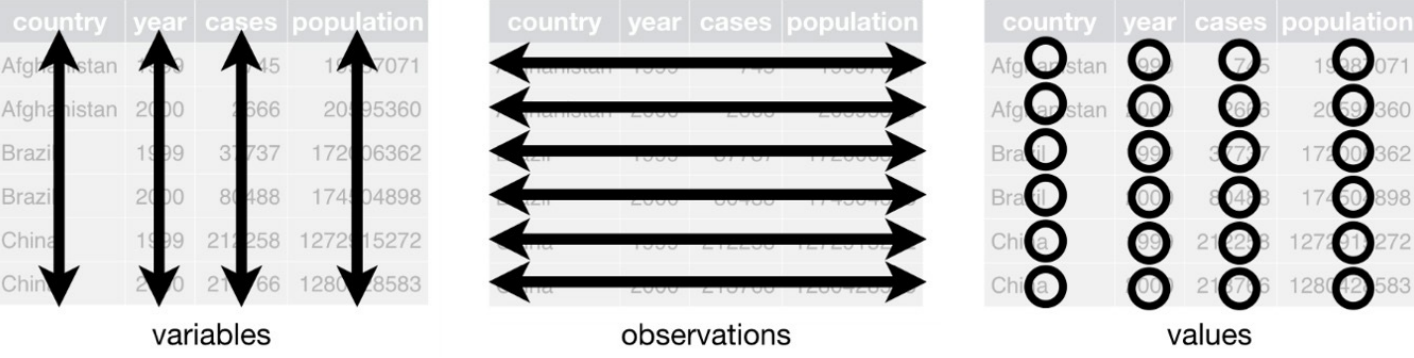
\includegraphics[width=1\linewidth]{images/figura1} 

}

\caption{Partes de los datos}\label{fig:figura1}
\end{figure}

\begin{itemize}
\tightlist
\item
  En primer lugar, tener una estructura de datos consistente es muy importante.\\
\item
  Los paquetes que forman parte de \texttt{tidyverse} (incluyendo \texttt{dplyr} y \texttt{ggplot2}) están diseñados para trabajar con datos ordenados.
\end{itemize}

{} Observación

Asegurar que tus datos sean uniformes facilita el procesamiento eficiente de tus datos.

\begin{itemize}
\item
  Además, colocar las variables en columnas permite facilitar la vectorización en \textbf{R}.
\item
  Muchos de los conjuntos de datos que encuentre no estarán ordenados y requerirán algo de trabajo por su parte.\\
  Puede haber muchas razones por las que un conjunto de datos no esté ordenado.\\
  A menudo, \textbf{las personas que crearon el conjunto de datos no están familiarizadas con los principios de los datos ordenados}.
\item
  Otra razón común por la que los conjuntos de datos no están ordenados es que los datos se organizan a menudo para facilitar algo más que el análisis.
\end{itemize}

{} Nota importante

Para que la introducción de datos sea lo más fácil posible, en ocasiones se suelen organizar los datos de forma poco ordenada.\\
Así, muchos conjuntos de datos requieren algún tipo de ordenación antes de poder empezar el análisis.

\begin{itemize}
\item
  El primer paso es averiguar cuáles son las variables y observaciones del conjunto de datos.\\
  Esto le facilitará la comprensión de lo que deben ser las columnas y las filas.
\item
  Además, también tendrá que resolver uno o dos problemas comunes:\\
  deberá \textbf{averiguar si una variable está repartida en varias columnas, y si una observación está dispersa en varias filas}.\\
  Estos conceptos se conocen como \textbf{reunión} y \textbf{dispersión}.
\end{itemize}

{} En esta sección veremos:

Recopilación

Distribución

Separación

Unión

\subsection{Recopilación}\label{recopilaciuxf3n}

\begin{itemize}
\tightlist
\item
  Un problema común en muchos conjuntos de datos es que los \textbf{nombres de las columnas no son variables sino valores de una variable}.\\
\item
  En la figura siguiente, las columnas 1999 y 2000 son en realidad valores de la variable \texttt{YEAR}.\\
\item
  \emph{Cada fila de la tabla existente representa en realidad dos observaciones}.
\end{itemize}

El paquete \texttt{tidyr} puede utilizarse para \textbf{reunir estas columnas existentes en una nueva variable}.\\
En este caso, tenemos que crear una nueva columna llamada \texttt{YEAR} y luego reunir en esta los valores existentes en las columnas 1999 y 2000.

\begin{figure}

{\centering 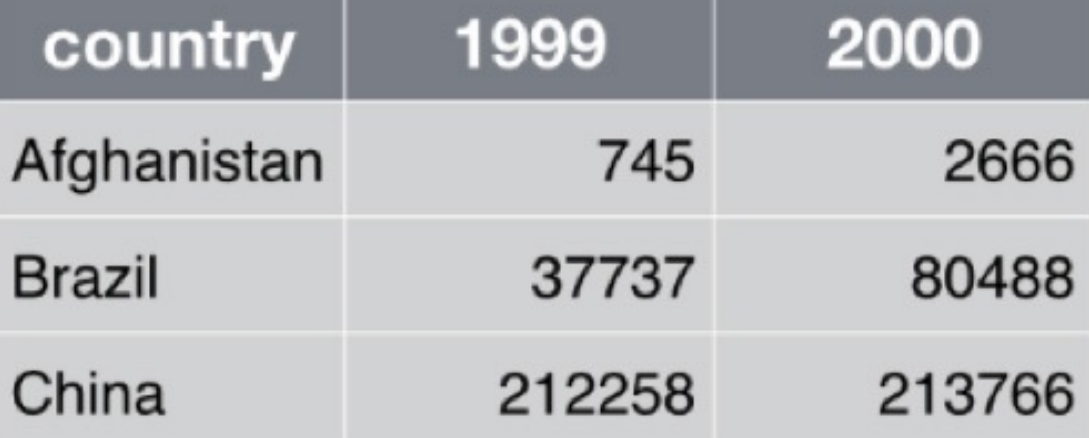
\includegraphics[width=1\linewidth]{images/figura2} 

}

\caption{Partes de los datos}\label{fig:figura2}
\end{figure}

{} Definición de gather()

La función gather() del paquete tidyr se utiliza para transformar datos de un formato
ancho (wide) a un formato largo (long).\\
Su objetivo principal es reunir varias columnas en una sola, creando una nueva variable que identifica
los nombres de las columnas originales y otra que contiene los valores asociados.

En otras palabras, gather() permite convertir columnas que representan valores en
filas ordenadas, lo que facilita el análisis de datos bajo los principios de datos ordenados.

{} Ejemplo práctico

En este ejercicio aprenderás a utilizar la función gather() para realizar la tarea de ordenación de datos.

Descargue el archivo CountryPopulation.csv localizado en
RDataSets.

Solución

\begin{itemize}
\tightlist
\item
  A continuación, tendrás que \textbf{nombrar la variable de la nueva columna}. Esto también se llama la clave \texttt{key}, y en este caso será la variable del año (\texttt{year}). Por último, tendrás que proporcionar el valor \texttt{value}, que es el \textbf{nombre de la variable cuyos valores se reparten por las celdas}.
\end{itemize}

\begin{figure}

{\centering 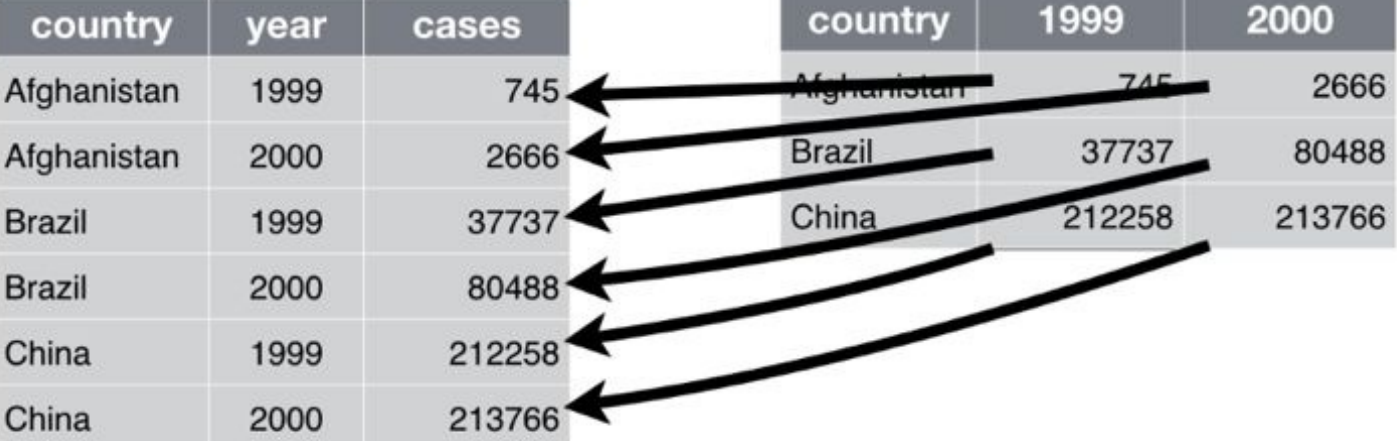
\includegraphics[width=1\linewidth]{images/figura4} 

}

\caption{Ilustraci<U+00F3>n de la funci<U+00F3>n gather}\label{fig:figura3}
\end{figure}

\begin{itemize}
\tightlist
\item
  Carguemos los datos
\end{itemize}

\begin{Shaded}
\begin{Highlighting}[]
\FunctionTok{library}\NormalTok{(tidyverse)}

\NormalTok{df }\OtherTok{=} \FunctionTok{read\_csv}\NormalTok{(}\StringTok{"data/CountryPopulation.csv"}\NormalTok{)}
\FunctionTok{head}\NormalTok{(df,}\AttributeTok{n=}\DecValTok{5}\NormalTok{)}
\end{Highlighting}
\end{Shaded}

\begin{verbatim}
## # A tibble: 5 x 10
##   `Country Name` `Country Code`   `2010`  `2011` `2012` `2013` `2014`
##   <chr>          <chr>             <dbl>   <dbl>  <dbl>  <dbl>  <dbl>
## 1 Aruba          ABW              101669  1.02e5 1.03e5 1.03e5 1.04e5
## 2 Afghanistan    AFG            28803167  2.97e7 3.07e7 3.17e7 3.28e7
## 3 Angola         AGO            23369131  2.42e7 2.51e7 2.60e7 2.69e7
## 4 Albania        ALB             2913021  2.91e6 2.90e6 2.90e6 2.89e6
## 5 Andorra        AND               84449  8.38e4 8.24e4 8.08e4 7.92e4
## # i 3 more variables: `2015` <dbl>, `2016` <dbl>, `2017` <dbl>
\end{verbatim}

\begin{itemize}
\tightlist
\item
  Utilice la función \texttt{gather} como se ve a continuación
\end{itemize}

\begin{Shaded}
\begin{Highlighting}[]
\NormalTok{df2 }\OtherTok{=} \FunctionTok{gather}\NormalTok{(df, }
                \StringTok{"2010"}\NormalTok{, }\StringTok{"2011"}\NormalTok{, }\StringTok{"2012"}\NormalTok{, }\StringTok{"2013"}\NormalTok{, }\StringTok{"2014"}\NormalTok{, }\StringTok{"2015"}\NormalTok{, }\StringTok{"2016"}\NormalTok{, }\StringTok{"2017"}\NormalTok{, }
                \AttributeTok{key =} \StringTok{"YEAR"}\NormalTok{, }
                \AttributeTok{value =} \StringTok{"POPULATION"}\NormalTok{)}
\NormalTok{knitr}\SpecialCharTok{::}\FunctionTok{kable}\NormalTok{(}\FunctionTok{head}\NormalTok{(df2, }\DecValTok{5}\NormalTok{))}
\end{Highlighting}
\end{Shaded}

\begin{tabular}{l|l|l|r}
\hline
Country Name & Country Code & YEAR & POPULATION\\
\hline
Aruba & ABW & 2010 & 101669\\
\hline
Afghanistan & AFG & 2010 & 28803167\\
\hline
Angola & AGO & 2010 & 23369131\\
\hline
Albania & ALB & 2010 & 2913021\\
\hline
Andorra & AND & 2010 & 84449\\
\hline
\end{tabular}

\begin{itemize}
\tightlist
\item
  Otra opción también sería la siguiente, cuando contamos con un gran número de columnas de este tipo, debemos usar la \textbf{expresiones regulares}.
\end{itemize}

\begin{Shaded}
\begin{Highlighting}[]
\NormalTok{years }\OtherTok{\textless{}{-}} \FunctionTok{colnames}\NormalTok{(df)[}\FunctionTok{grep}\NormalTok{(}\StringTok{"\^{}}\SpecialCharTok{\textbackslash{}\textbackslash{}}\StringTok{d\{4\}$"}\NormalTok{, }\FunctionTok{colnames}\NormalTok{(df))]}

\NormalTok{df2 }\OtherTok{\textless{}{-}}\NormalTok{ df }\SpecialCharTok{\%\textgreater{}\%}
  \FunctionTok{gather}\NormalTok{(}\AttributeTok{key =} \StringTok{"YEAR"}\NormalTok{, }\AttributeTok{value =} \StringTok{"POPULATION"}\NormalTok{, }\FunctionTok{all\_of}\NormalTok{(years))}

\NormalTok{knitr}\SpecialCharTok{::}\FunctionTok{kable}\NormalTok{(}\FunctionTok{head}\NormalTok{(df2, }\DecValTok{5}\NormalTok{))}
\end{Highlighting}
\end{Shaded}

\begin{tabular}{l|l|l|r}
\hline
Country Name & Country Code & YEAR & POPULATION\\
\hline
Aruba & ABW & 2010 & 101669\\
\hline
Afghanistan & AFG & 2010 & 28803167\\
\hline
Angola & AGO & 2010 & 23369131\\
\hline
Albania & ALB & 2010 & 2913021\\
\hline
Andorra & AND & 2010 & 84449\\
\hline
\end{tabular}

\begin{itemize}
\item
  Donde, en \emph{expresiones regulares}, \texttt{"\^{}\textbackslash{}\textbackslash{}d\{4\}\$"} tiene el siguiente significado:

  \begin{itemize}
  \tightlist
  \item
    \texttt{\^{}} : Representa el inicio de una cadena.\\
  \item
    \texttt{\textbackslash{}\textbackslash{}d} : Representa un dígito.\\
  \item
    \texttt{\{4\}} : Indica que el elemento anterior (\texttt{\textbackslash{}\textbackslash{}d}, en este caso) debe aparecer exactamente 4 veces.\\
  \item
    \texttt{\$} : Representa el final de una cadena.
  \end{itemize}
\item
  En resumen, \texttt{"\^{}\textbackslash{}\textbackslash{}d\{4\}\$"} coincide con cualquier \textbf{cadena que contenga exactamente 4 dígitos y no contenga ningún otro carácter adicional antes o después de los dígitos}.
\end{itemize}

\subsection{Distribución}\label{distribuciuxf3n}

{} Concepto

La distribución es el proceso opuesto a la reunión y
se aplica cuando una sola observación está fragmentada en varias filas.\\
Su objetivo es reorganizar los datos para que cada observación quede contenida en una única fila.

\begin{itemize}
\tightlist
\item
  En el diagrama siguiente, la tabla debería definir una observación de un país por año. Sin embargo, se observa que está repartida en dos filas: una para cases y otra para population.
\end{itemize}

\begin{figure}

{\centering 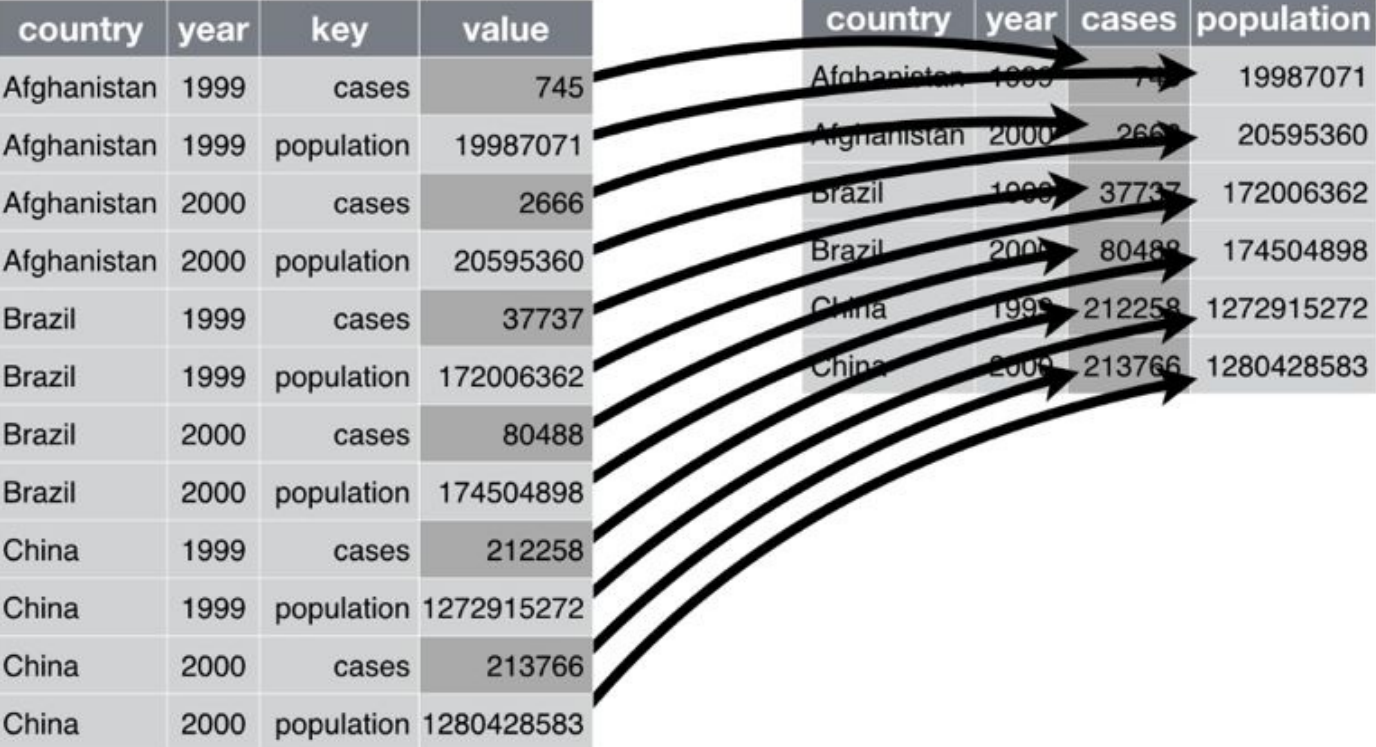
\includegraphics[width=1\linewidth]{images/figura5} 

}

\caption{Distribuci<U+00F3>n}\label{fig:figura5}
\end{figure}

\begin{itemize}
\tightlist
\item
  Para solucionar este problema, podemos utilizar la función \texttt{spread()} del paquete \texttt{tidyr}.
\end{itemize}

{} Definición: Sintaxis de spread()

La función spread() del paquete tidyr se utiliza para transformar un conjunto de datos
de formato largo (long) a formato ancho (wide).\\
Su propósito es distribuir los valores de una variable en varias columnas.

Toma dos parámetros principales:

key: columna que contiene los nombres de las variables que se convertirán en nuevas columnas.

value: columna que contiene los valores que se ubicarán en las nuevas celdas.

\begin{itemize}
\tightlist
\item
  Instale el paquete \texttt{devtools} y los conjuntos de datos \textbf{DSR} utilizando el código que ve a continuación escribiendo en el panel de la consola. Alternativamente, puede utilizar el panel de paquetes para instalar los librerías
\end{itemize}

\begin{Shaded}
\begin{Highlighting}[]
\CommentTok{\# Instalar }
\CommentTok{\# install.packages("devtools")}
\CommentTok{\# devtools::install\_github("garrettgman/DSR")}
\FunctionTok{library}\NormalTok{(devtools)}
\end{Highlighting}
\end{Shaded}

\begin{itemize}
\tightlist
\item
  Tomemos los datos de \texttt{table2}:
\end{itemize}

\begin{Shaded}
\begin{Highlighting}[]
\NormalTok{knitr}\SpecialCharTok{::}\FunctionTok{kable}\NormalTok{(}\FunctionTok{head}\NormalTok{(table2))}
\end{Highlighting}
\end{Shaded}

\begin{tabular}{l|r|l|r}
\hline
country & year & type & count\\
\hline
Afghanistan & 1999 & cases & 745\\
\hline
Afghanistan & 1999 & population & 19987071\\
\hline
Afghanistan & 2000 & cases & 2666\\
\hline
Afghanistan & 2000 & population & 20595360\\
\hline
Brazil & 1999 & cases & 37737\\
\hline
Brazil & 1999 & population & 172006362\\
\hline
\end{tabular}

\begin{itemize}
\tightlist
\item
  Utilice la función \texttt{spread()} para corregir este problema.
\end{itemize}

\begin{Shaded}
\begin{Highlighting}[]
\NormalTok{table2b }\OtherTok{=} \FunctionTok{spread}\NormalTok{(table2, }\AttributeTok{key =}\NormalTok{ type, }\AttributeTok{value =}\NormalTok{ count)}
\NormalTok{knitr}\SpecialCharTok{::}\FunctionTok{kable}\NormalTok{(}\FunctionTok{head}\NormalTok{(table2b))}
\end{Highlighting}
\end{Shaded}

\begin{tabular}{l|r|r|r}
\hline
country & year & cases & population\\
\hline
Afghanistan & 1999 & 745 & 19987071\\
\hline
Afghanistan & 2000 & 2666 & 20595360\\
\hline
Brazil & 1999 & 37737 & 172006362\\
\hline
Brazil & 2000 & 80488 & 174504898\\
\hline
China & 1999 & 212258 & 1272915272\\
\hline
China & 2000 & 213766 & 1280428583\\
\hline
\end{tabular}

\subsection{Separación}\label{separaciuxf3n}

Otro caso común es el de dos variables que se colocan en la misma columna. Por ejemplo, la hoja de cálculo siguiente tiene una columna \textbf{State-County Name} que en realidad contiene dos variables separadas por una barra.

\begin{figure}

{\centering 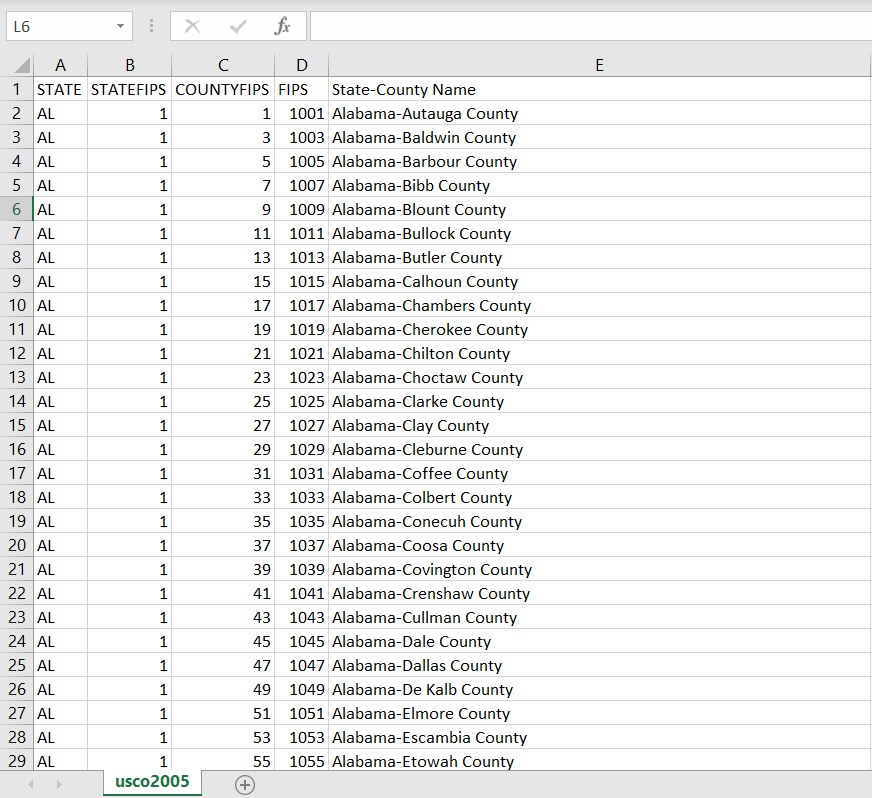
\includegraphics[width=1\linewidth]{images/figura6} 

}

\caption{DataSet}\label{fig:figura6}
\end{figure}

La función \texttt{separate()} puede utilizarse para dividir una columna en varias columnas dividiendo por un separador. Por defecto, la función \texttt{separate()} buscará automáticamente cualquier carácter no alfanumérico o se puede definir un carácter específico (ver \href{https://www.rdocumentation.org/packages/tidyr/versions/1.3.0/topics/separate}{separate()}).

\begin{itemize}
\tightlist
\item
  En la carpeta de \textbf{RDataSets} hay un archivo llamado \textbf{usco2005.csv}. Abra este archivo, por ejemplo con Microsoft Excel, o algún otro tipo de software de hoja de cálculo. El archivo debería tener un aspecto similar al de la captura de pantalla de abajo.
\end{itemize}

\begin{figure}

{\centering 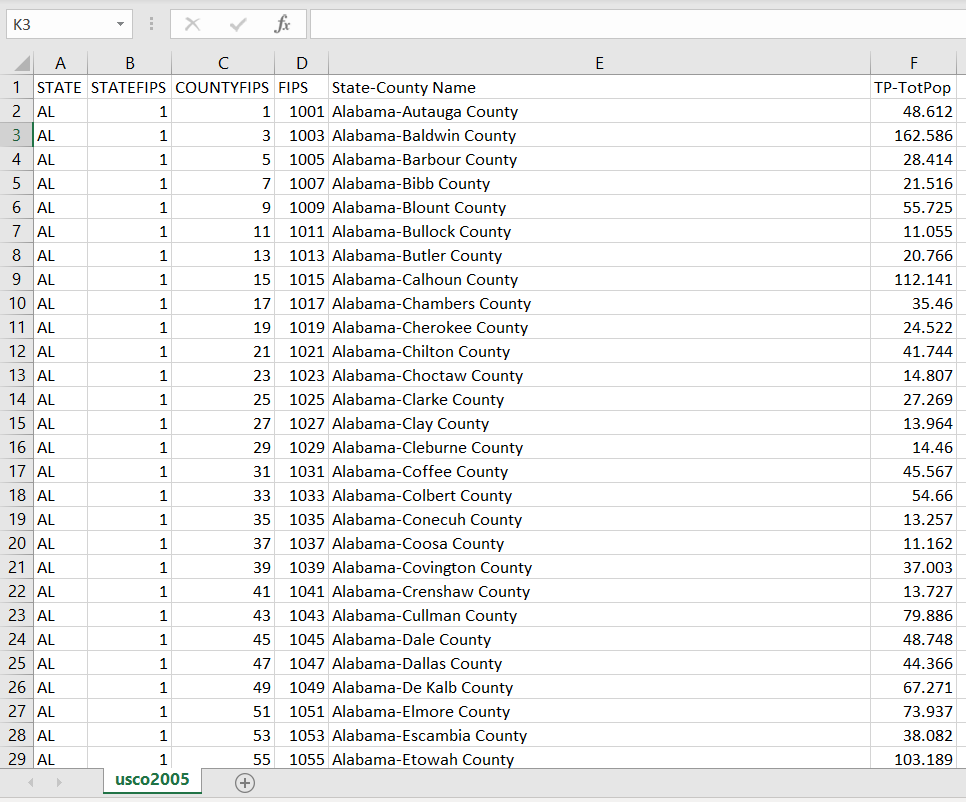
\includegraphics[width=1\linewidth]{images/figura7} 

}

\caption{DataSet de usco2005}\label{fig:figura7}
\end{figure}

\begin{itemize}
\tightlist
\item
  Cargue el archivo \textbf{usco2005.csv} en \textbf{RStudio} escribiendo el código que ve a continuación en el panel de la consola
\end{itemize}

\begin{Shaded}
\begin{Highlighting}[]
\NormalTok{df }\OtherTok{=} \FunctionTok{read\_csv}\NormalTok{(}\StringTok{"data/usco2005.csv"}\NormalTok{)}
\NormalTok{knitr}\SpecialCharTok{::}\FunctionTok{kable}\NormalTok{(}\FunctionTok{head}\NormalTok{(df, }\DecValTok{5}\NormalTok{))}
\end{Highlighting}
\end{Shaded}

\begin{tabular}{l|r|r|r|l|r}
\hline
STATE & STATEFIPS & COUNTYFIPS & FIPS & State-County Name & TP-TotPop\\
\hline
AL & 1 & 1 & 1001 & Alabama-Autauga County & 48.612\\
\hline
AL & 1 & 3 & 1003 & Alabama-Baldwin County & 162.586\\
\hline
AL & 1 & 5 & 1005 & Alabama-Barbour County & 28.414\\
\hline
AL & 1 & 7 & 1007 & Alabama-Bibb County & 21.516\\
\hline
AL & 1 & 9 & 1009 & Alabama-Blount County & 55.725\\
\hline
\end{tabular}

\begin{itemize}
\tightlist
\item
  Utilice la función \texttt{separate()} para separar el contenido de la columna \textbf{State-County Name} en las columnas \textbf{StateAbbrev} y \textbf{CountyName}
\end{itemize}

\begin{Shaded}
\begin{Highlighting}[]
\NormalTok{df2 }\OtherTok{=} \FunctionTok{separate}\NormalTok{(df, }\StringTok{"State{-}County Name"}\NormalTok{,}\AttributeTok{into =} \FunctionTok{c}\NormalTok{(}\StringTok{"StateAbbrev"}\NormalTok{, }\StringTok{"CountyName"}\NormalTok{))}
\NormalTok{knitr}\SpecialCharTok{::}\FunctionTok{kable}\NormalTok{(}\FunctionTok{head}\NormalTok{(df2, }\DecValTok{5}\NormalTok{))}
\end{Highlighting}
\end{Shaded}

\begin{tabular}{l|r|r|r|l|l|r}
\hline
STATE & STATEFIPS & COUNTYFIPS & FIPS & StateAbbrev & CountyName & TP-TotPop\\
\hline
AL & 1 & 1 & 1001 & Alabama & Autauga & 48.612\\
\hline
AL & 1 & 3 & 1003 & Alabama & Baldwin & 162.586\\
\hline
AL & 1 & 5 & 1005 & Alabama & Barbour & 28.414\\
\hline
AL & 1 & 7 & 1007 & Alabama & Bibb & 21.516\\
\hline
AL & 1 & 9 & 1009 & Alabama & Blount & 55.725\\
\hline
\end{tabular}

\subsection{Unión}\label{uniuxf3n}

{} Definición

unite() de tidyr combina varias columnas en una sola,
aplicando un separador entre los valores. Es, conceptualmente, la operación inversa de separate().

{} Parámetros clave

data: marco de datos.

col: nombre de la nueva columna combinada.

\ldots{}: columnas a unir (en el orden deseado).

sep: separador entre valores (por defecto ``\_``).

remove: si TRUE, elimina las columnas originales.

na.rm: si TRUE, omite NA al unir; si FALSE, el resultado será NA si alguna parte es NA.

Sintaxis: unite(data, col, \ldots, sep = ``\_``, remove = TRUE, na.rm = FALSE)

\begin{Shaded}
\begin{Highlighting}[]
\NormalTok{df3 }\OtherTok{=} \FunctionTok{unite}\NormalTok{(df2, State\_County\_Name, StateAbbrev, CountyName)}
\NormalTok{knitr}\SpecialCharTok{::}\FunctionTok{kable}\NormalTok{(}\FunctionTok{head}\NormalTok{(df3, }\DecValTok{5}\NormalTok{))}
\end{Highlighting}
\end{Shaded}

\begin{tabular}{l|r|r|r|l|r}
\hline
STATE & STATEFIPS & COUNTYFIPS & FIPS & State\_County\_Name & TP-TotPop\\
\hline
AL & 1 & 1 & 1001 & Alabama\_Autauga & 48.612\\
\hline
AL & 1 & 3 & 1003 & Alabama\_Baldwin & 162.586\\
\hline
AL & 1 & 5 & 1005 & Alabama\_Barbour & 28.414\\
\hline
AL & 1 & 7 & 1007 & Alabama\_Bibb & 21.516\\
\hline
AL & 1 & 9 & 1009 & Alabama\_Blount & 55.725\\
\hline
\end{tabular}

{} Ejercicio para entregar

Considere el conjunto de datos \href{https://github.com/cdeoroaguado/Datos/blob/main/datapython/us_state_population.tsv}{us\_state\_population.tsv} ubicado en la carpeta de datos de Python de github. Repita el procedimiento planteado en cada ítem de esta sección para obtener el nuevo dataframe con las nuevas columnas \texttt{Year} y \texttt{Population}. Realice unión y separación utilizando las columnas \texttt{State} y \texttt{Code}.

\chapter{Exploración y visualización estática de datos}\label{vizestatico}

{} Definición: Análisis Exploratorio de Datos (EDA)

El Análisis Exploratorio de Datos (EDA) es un flujo de trabajo diseñado para obtener una mejor comprensión de los datos.
Se desarrolla en tres pasos:

El primero consiste en generar preguntas sobre los datos. En este paso se quiere ser lo más amplio posible, ya que en este momento no se tiene una buena idea de los datos.

A continuación, se buscan las respuestas a estas preguntas mediante la visualización, la transformación y el modelado de los datos.

Por último, refine sus preguntas o genere nuevas preguntas.

{} Definición: Tipos de variables en R

Los datos pueden dividirse en dos grandes grupos:

Variables con datos categóricas: Conjunto reducido de valores discretos. Ejemplo: sexo, país, color.

Variables con datos numéricos: Conjunto potencialmente infinito de valores numéricos ordenados. Ejemplo: peso, edad, estatura.

{} Visualización de variables

Las categóricas suelen representarse con gráficos de barras.

Las numéricas se visualizan con histogramas, boxplots.

Tanto categóricas como continuas también pueden representarse mediante gráficos creados en R.

{} Definición: Variación y Covariación

Variación: grado en que los valores de una misma variable cambian entre distintas observaciones o mediciones.

Covariación: describe cómo cambian conjuntamente los valores de dos o más variables, es decir, la medida en que la variación de una se asocia con la variación de otra.

{} Técnicas básicas de exploración gráfica

Medir variación categórica con gráfico de barras.

Medir variación continua con histograma.

Medir covariación con diagramas de caja.

Medir covariación mediante tamaño de símbolos en gráficos de dispersión.

Creación de gráficos 2D y mapas de calor (hexbin).

Generación de estadísticas de resumen.

\section{Visualización de variables categóricas con gráficos de barras}\label{visualizaciuxf3n-de-variables-categuxf3ricas-con-gruxe1ficos-de-barras}

Un gráfico de barras es una buena manera de visualizar datos categóricos. Se separa cada categoría en una barra separada y la altura de cada barra se define por el número de ocurrencias en esa categoría.

Para los ejercicios de esta sección requieren los siguientes paquetes: \texttt{readr,\ dplyr,\ ggplot2}. Pueden cargarse desde el panel de paquetes, el panel de la consola o un script. Estos paquetes estan en el paquete de \texttt{tidyverse}.

\begin{itemize}
\tightlist
\item
  Utilice la función \texttt{read\_csv()} para cargar el conjunto de datos de incendios forestales en un marco \textbf{dataframe}.
\end{itemize}

\begin{Shaded}
\begin{Highlighting}[]
\FunctionTok{library}\NormalTok{(dplyr)}
\FunctionTok{library}\NormalTok{(readr)}
\FunctionTok{library}\NormalTok{(ggplot2)}

\NormalTok{datos }\OtherTok{\textless{}{-}} \FunctionTok{read\_csv}\NormalTok{(}\StringTok{"data/StudyArea.csv"}\NormalTok{)}
\end{Highlighting}
\end{Shaded}

\begin{itemize}
\tightlist
\item
  Visualicemos las 5 primeras observaciones
\end{itemize}

\begin{Shaded}
\begin{Highlighting}[]
\FunctionTok{head}\NormalTok{(datos)}
\end{Highlighting}
\end{Shaded}

\begin{verbatim}
## # A tibble: 6 x 14
##     FID ORGANIZATI UNIT  SUBUNIT SUBUNIT2        FIRENAME CAUSE YEAR_
##   <dbl> <chr>      <chr> <chr>   <chr>           <chr>    <chr> <dbl>
## 1     0 FWS        81682 USCADBR San Diego Bay ~ PUMP HO~ Human  2001
## 2     1 FWS        81682 USCADBR San Diego Bay ~ I5       Human  2002
## 3     2 FWS        81682 USCADBR San Diego Bay ~ SOUTHBAY Human  2002
## 4     3 FWS        81682 USCADBR San Diego Bay ~ MARINA   Human  2001
## 5     4 FWS        81682 USCADBR San Diego Bay ~ HILL     Human  1994
## 6     5 FWS        81682 USCADBR San Diego Bay ~ IRRIGAT~ Human  1994
## # i 6 more variables: STARTDATED <chr>, CONTRDATED <chr>,
## #   OUTDATED <chr>, STATE <chr>, STATE_FIPS <dbl>, TOTALACRES <dbl>
\end{verbatim}

\begin{itemize}
\tightlist
\item
  Ahora, la estructura de los datos
\end{itemize}

\begin{Shaded}
\begin{Highlighting}[]
\FunctionTok{str}\NormalTok{(datos)}
\end{Highlighting}
\end{Shaded}

\begin{verbatim}
## spc_tbl_ [439,362 x 14] (S3: spec_tbl_df/tbl_df/tbl/data.frame)
##  $ FID       : num [1:439362] 0 1 2 3 4 5 6 18 20 21 ...
##  $ ORGANIZATI: chr [1:439362] "FWS" "FWS" "FWS" "FWS" ...
##  $ UNIT      : chr [1:439362] "81682" "81682" "81682" "81682" ...
##  $ SUBUNIT   : chr [1:439362] "USCADBR" "USCADBR" "USCADBR" "USCADBR" ...
##  $ SUBUNIT2  : chr [1:439362] "San Diego Bay National Wildlife Refuge" "San Diego Bay National Wildlife Refuge" "San Diego Bay National Wildlife Refuge" "San Diego Bay National Wildlife Refuge" ...
##  $ FIRENAME  : chr [1:439362] "PUMP HOUSE" "I5" "SOUTHBAY" "MARINA" ...
##  $ CAUSE     : chr [1:439362] "Human" "Human" "Human" "Human" ...
##  $ YEAR_     : num [1:439362] 2001 2002 2002 2001 1994 ...
##  $ STARTDATED: chr [1:439362] "1/1/01 0:00" "5/3/02 0:00" "6/1/02 0:00" "7/12/01 0:00" ...
##  $ CONTRDATED: chr [1:439362] "1/1/01 0:00" "5/3/02 0:00" "6/1/02 0:00" "7/12/01 0:00" ...
##  $ OUTDATED  : chr [1:439362] NA NA NA NA ...
##  $ STATE     : chr [1:439362] "California" "California" "California" "California" ...
##  $ STATE_FIPS: num [1:439362] 6 6 6 6 6 6 6 6 6 6 ...
##  $ TOTALACRES: num [1:439362] 0.1 3 0.5 0.1 1 0.1 3 0.1 0.1 0.1 ...
##  - attr(*, "spec")=
##   .. cols(
##   ..   FID = col_double(),
##   ..   ORGANIZATI = col_character(),
##   ..   UNIT = col_character(),
##   ..   SUBUNIT = col_character(),
##   ..   SUBUNIT2 = col_character(),
##   ..   FIRENAME = col_character(),
##   ..   CAUSE = col_character(),
##   ..   YEAR_ = col_double(),
##   ..   STARTDATED = col_character(),
##   ..   CONTRDATED = col_character(),
##   ..   OUTDATED = col_character(),
##   ..   STATE = col_character(),
##   ..   STATE_FIPS = col_double(),
##   ..   TOTALACRES = col_double()
##   .. )
##  - attr(*, "problems")=<externalptr>
\end{verbatim}

\begin{itemize}
\tightlist
\item
  Para este análisis, filtraremos los datos de modo que solo estén representados los incendios que quemaron más de 1000 acres (4046.86 metros cuadrados o 0.4047 hectáreas) en los años 2010 a 2016.
\end{itemize}

\begin{Shaded}
\begin{Highlighting}[]
\NormalTok{df }\OtherTok{\textless{}{-}}\NormalTok{  datos }\SpecialCharTok{\%\textgreater{}\%} 
  \FunctionTok{filter}\NormalTok{(TOTALACRES }\SpecialCharTok{\textgreater{}=} \DecValTok{1000}\NormalTok{,}
\NormalTok{         YEAR\_ }\SpecialCharTok{\%in\%} \FunctionTok{c}\NormalTok{(}\DecValTok{2010}\NormalTok{, }\DecValTok{2011}\NormalTok{, }\DecValTok{2012}\NormalTok{, }\DecValTok{2013}\NormalTok{, }\DecValTok{2014}\NormalTok{, }\DecValTok{2015}\NormalTok{, }\DecValTok{2016}\NormalTok{))}
\end{Highlighting}
\end{Shaded}

\begin{itemize}
\tightlist
\item
  Añada el código que que se ve a continuación para filtrar los datos y enviar los resultados a un gráfico de barras.
\end{itemize}

\begin{Shaded}
\begin{Highlighting}[]
\NormalTok{df }\SpecialCharTok{\%\textgreater{}\%} 
  \FunctionTok{ggplot}\NormalTok{(}\AttributeTok{mapping =} \FunctionTok{aes}\NormalTok{(}\AttributeTok{x =}\NormalTok{ YEAR\_)) }\SpecialCharTok{+} 
  \FunctionTok{geom\_bar}\NormalTok{() }\SpecialCharTok{+}
  \FunctionTok{scale\_x\_continuous}\NormalTok{(}\AttributeTok{breaks =} \FunctionTok{c}\NormalTok{(}\DecValTok{2010}\NormalTok{, }\DecValTok{2011}\NormalTok{, }\DecValTok{2012}\NormalTok{, }\DecValTok{2013}\NormalTok{, }\DecValTok{2014}\NormalTok{, }\DecValTok{2015}\NormalTok{, }\DecValTok{2016}\NormalTok{)) }\SpecialCharTok{+}
  \FunctionTok{labs}\NormalTok{(}\AttributeTok{x =} \StringTok{\textquotesingle{}Años\textquotesingle{}}\NormalTok{,}
       \AttributeTok{y =} \StringTok{\textquotesingle{}Número de incendios\textquotesingle{}}\NormalTok{) }\OtherTok{{-}\textgreater{}}\NormalTok{ barras}

\NormalTok{barras}
\end{Highlighting}
\end{Shaded}

\pandocbounded{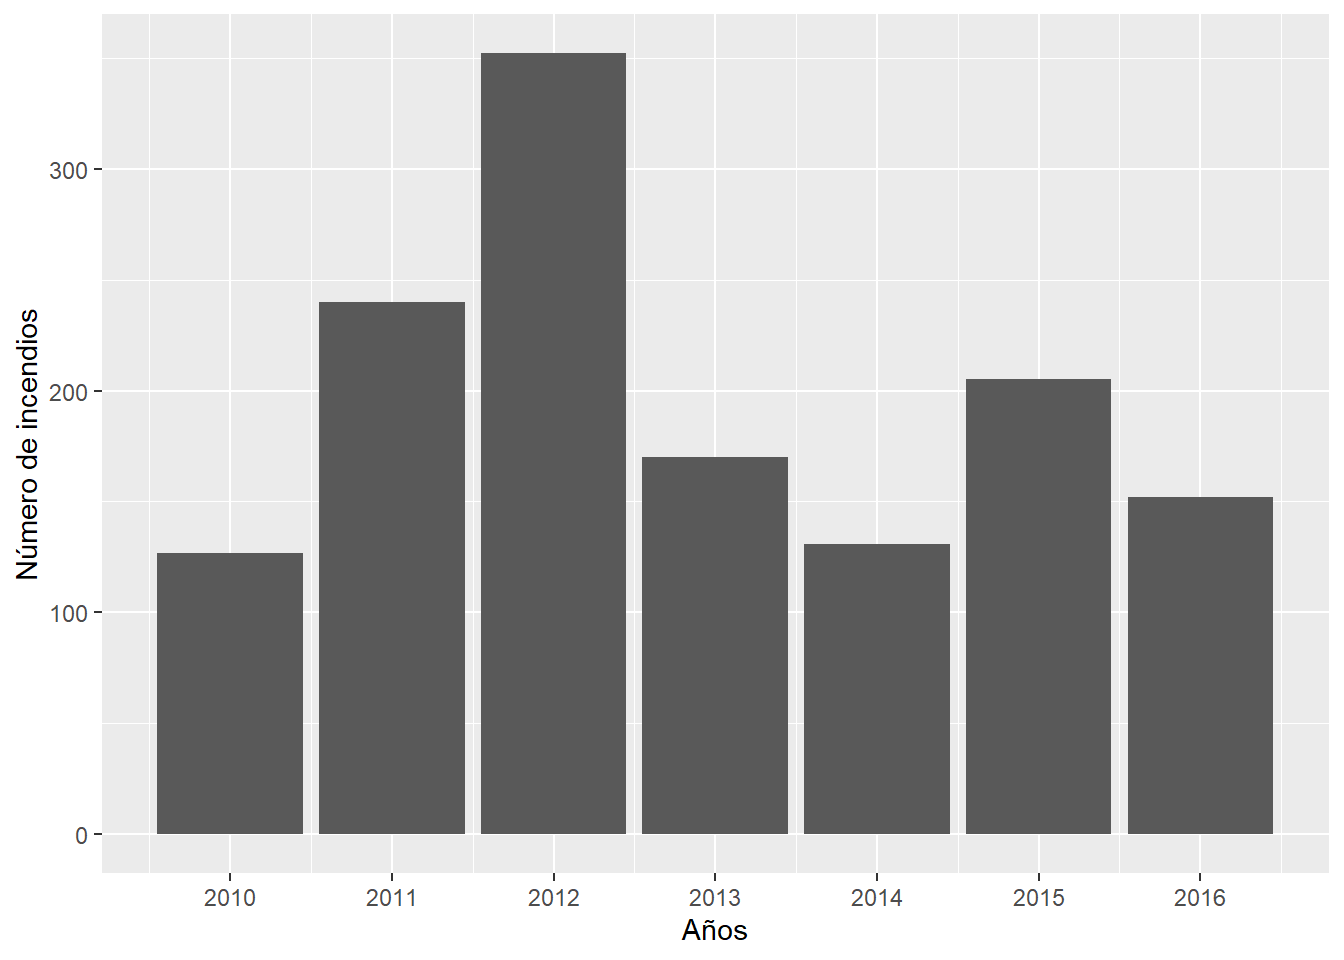
\includegraphics[keepaspectratio]{bookdown-demo_files/figure-latex/barra_vizest-1.pdf}}

\begin{itemize}
\tightlist
\item
  Si queremos incorporar temáticas para una mejor visualización, tenemos 8 temas que estan incluidos en ggplot2, los cuales son \texttt{theme\_bw}, \texttt{theme\_classic}, \texttt{theme\_dark}, \texttt{theme\_gray}, \texttt{theme\_light}, \texttt{theme\_linedraw}, \texttt{theme\_minimal}, \texttt{theme\_void}. Añade el código que ves a continuación para cambiar la faceta a \texttt{theme\_bw}.
\end{itemize}

\begin{Shaded}
\begin{Highlighting}[]
\NormalTok{barras}\SpecialCharTok{+}
  \FunctionTok{theme\_bw}\NormalTok{()}
\end{Highlighting}
\end{Shaded}

\pandocbounded{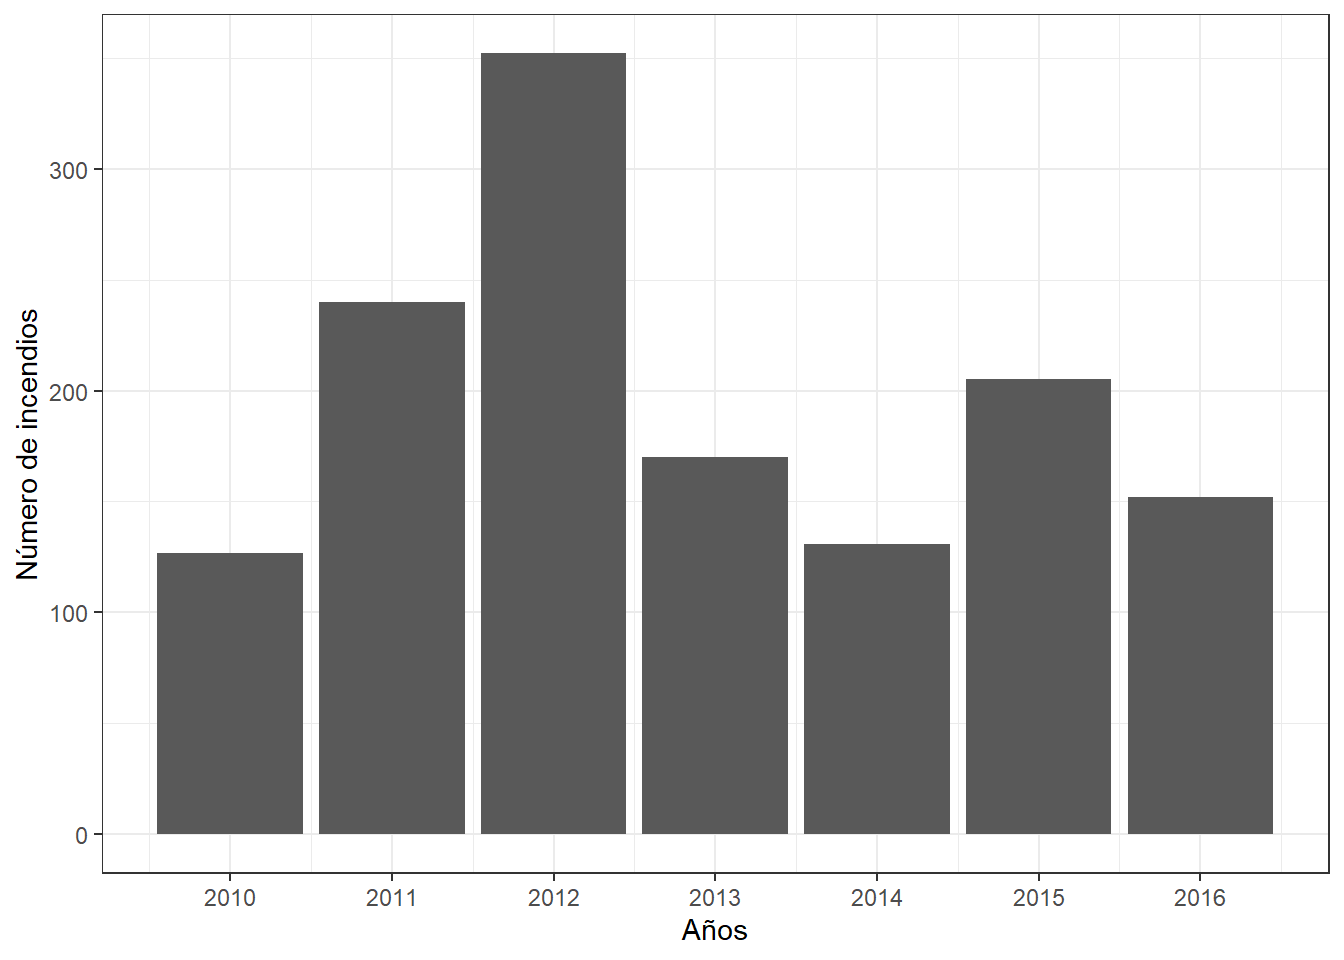
\includegraphics[keepaspectratio]{bookdown-demo_files/figure-latex/barra2_vizest-1.pdf}}

\begin{itemize}
\tightlist
\item
  Otra forma de realizar el gráfico de barras es la siguiente
\end{itemize}

\begin{Shaded}
\begin{Highlighting}[]
\NormalTok{df }\SpecialCharTok{\%\textgreater{}\%} 
  \FunctionTok{filter}\NormalTok{(TOTALACRES }\SpecialCharTok{\textgreater{}=} \DecValTok{1000}\NormalTok{,}
\NormalTok{         YEAR\_ }\SpecialCharTok{\%in\%} \FunctionTok{c}\NormalTok{(}\DecValTok{2010}\NormalTok{, }\DecValTok{2011}\NormalTok{, }\DecValTok{2012}\NormalTok{, }\DecValTok{2013}\NormalTok{, }\DecValTok{2014}\NormalTok{, }\DecValTok{2015}\NormalTok{, }\DecValTok{2016}\NormalTok{)) }\SpecialCharTok{\%\textgreater{}\%} 
  \FunctionTok{count}\NormalTok{(YEAR\_) }\SpecialCharTok{\%\textgreater{}\%} 
  \FunctionTok{mutate}\NormalTok{(}\AttributeTok{Porcentaje =}\NormalTok{ (n }\SpecialCharTok{/} \FunctionTok{sum}\NormalTok{(n))}\SpecialCharTok{*}\DecValTok{100}\NormalTok{) }\SpecialCharTok{\%\textgreater{}\%} 
  \FunctionTok{ggplot}\NormalTok{(}\AttributeTok{mapping =} \FunctionTok{aes}\NormalTok{(}\AttributeTok{x =} \FunctionTok{factor}\NormalTok{(YEAR\_),}\AttributeTok{y=}\NormalTok{n))}\SpecialCharTok{+}
  \FunctionTok{geom\_col}\NormalTok{(}\AttributeTok{fill =} \StringTok{"steelblue"}\NormalTok{) }\SpecialCharTok{+}
  \FunctionTok{geom\_text}\NormalTok{(}\FunctionTok{aes}\NormalTok{(}\AttributeTok{label =} \FunctionTok{paste0}\NormalTok{(n, }\StringTok{" ("}\NormalTok{, }\FunctionTok{round}\NormalTok{(Porcentaje,}\DecValTok{1}\NormalTok{), }\StringTok{"\%)"}\NormalTok{)),}
            \AttributeTok{vjust =} \SpecialCharTok{{-}}\FloatTok{0.5}\NormalTok{, }\AttributeTok{size =} \DecValTok{4}\NormalTok{) }\SpecialCharTok{+}
  \FunctionTok{labs}\NormalTok{(}\AttributeTok{x =} \StringTok{\textquotesingle{}Años\textquotesingle{}}\NormalTok{,}
       \AttributeTok{y =} \StringTok{\textquotesingle{}Número de incendios (\%)\textquotesingle{}}\NormalTok{)}\SpecialCharTok{+}
  \FunctionTok{theme\_bw}\NormalTok{()}
\end{Highlighting}
\end{Shaded}

\pandocbounded{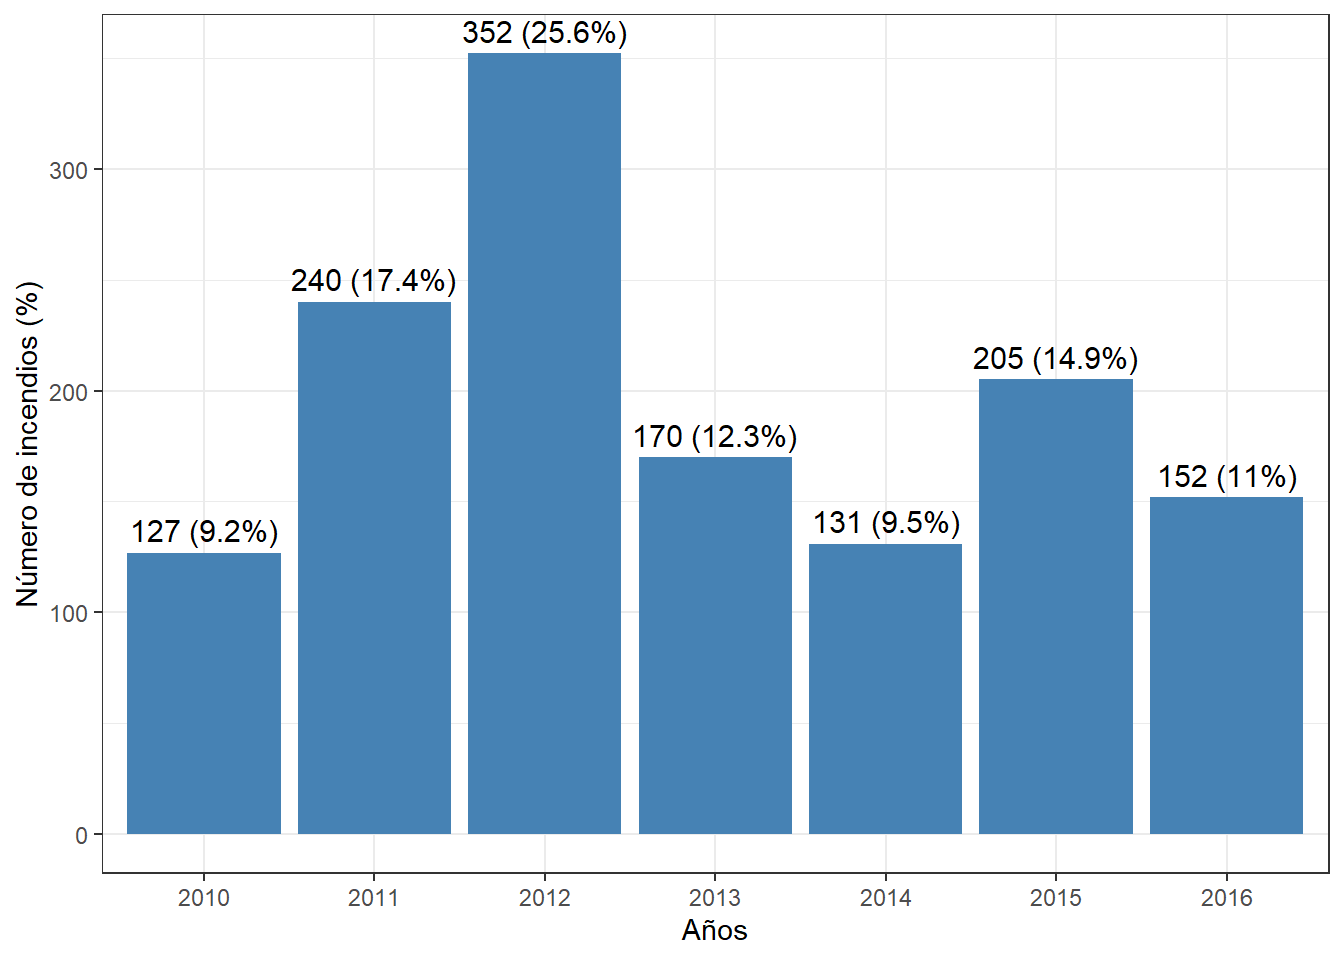
\includegraphics[keepaspectratio]{bookdown-demo_files/figure-latex/barra3_vizest-1.pdf}}

\section{Visualización de variable continua con un histograma}\label{visualizaciuxf3n-de-variable-continua-con-un-histograma}

La distribución de una variable continua se puede medir con el uso de un histograma. En este ejercicio crearás un histograma de los acres quemados en incendios forestales.

Siguiendo los datos de incendios forestales del 2010 al 2016:

\begin{itemize}
\tightlist
\item
  Introduzca el marco de datos y utilice la función \texttt{select()} para limitar las columnas y filtrar las filas para que sólo se incluyan los incendios superiores a 1.000 acres. Dado que tenemos un gran número de incendios forestales que quemaron sólo un pequeño número de acres, nos centraremos en los incendios que son un poco más grandes en este caso.
\end{itemize}

\begin{Shaded}
\begin{Highlighting}[]
\NormalTok{df }\SpecialCharTok{\%\textgreater{}\%}
  \FunctionTok{select}\NormalTok{(ORGANIZATI, STATE, YEAR\_, TOTALACRES, CAUSE) }\SpecialCharTok{\%\textgreater{}\%}
  \FunctionTok{filter}\NormalTok{(TOTALACRES }\SpecialCharTok{\textgreater{}=} \DecValTok{1000}\NormalTok{)}
\end{Highlighting}
\end{Shaded}

\begin{verbatim}
## # A tibble: 1,377 x 5
##    ORGANIZATI STATE      YEAR_ TOTALACRES CAUSE       
##    <chr>      <chr>      <dbl>      <dbl> <chr>       
##  1 FWS        Washington  2010       2755 Natural     
##  2 FWS        Idaho       2010       1801 Undetermined
##  3 FWS        Montana     2010      27898 Natural     
##  4 FWS        Montana     2012       9468 Natural     
##  5 FWS        Washington  2012       1141 Human       
##  6 FWS        Oregon      2010       3083 Human       
##  7 FWS        Oregon      2013      51015 Undetermined
##  8 FWS        Washington  2016     171915 Human       
##  9 FWS        Arizona     2015       6000 Natural     
## 10 FWS        Arizona     2016       1624 Natural     
## # i 1,367 more rows
\end{verbatim}

\begin{itemize}
\tightlist
\item
  Cree el histograma utilizando \texttt{ggplot()} con \texttt{geom\_hist()} y un tamaño de la celda de 500. Los datos están claramente sesgados hacia el extremo inferior del número de acres quemados.
\end{itemize}

\begin{Shaded}
\begin{Highlighting}[]
\NormalTok{df }\SpecialCharTok{\%\textgreater{}\%}
  \FunctionTok{select}\NormalTok{(ORGANIZATI, STATE, YEAR\_, TOTALACRES, CAUSE) }\SpecialCharTok{\%\textgreater{}\%}
  \FunctionTok{filter}\NormalTok{(TOTALACRES }\SpecialCharTok{\textgreater{}=} \DecValTok{1000}\NormalTok{) }\SpecialCharTok{\%\textgreater{}\%}
  \FunctionTok{slice}\NormalTok{(}\DecValTok{1}\SpecialCharTok{:}\DecValTok{300}\NormalTok{) }\SpecialCharTok{\%\textgreater{}\%}
  \FunctionTok{ggplot}\NormalTok{(}\AttributeTok{mapping =} \FunctionTok{aes}\NormalTok{(}\AttributeTok{x=}\NormalTok{TOTALACRES)) }\SpecialCharTok{+} 
  \FunctionTok{geom\_histogram}\NormalTok{( }\AttributeTok{binwidth=}\DecValTok{1000}\NormalTok{, }\AttributeTok{fill =} \StringTok{"steelblue"}\NormalTok{) }\SpecialCharTok{+}
  \FunctionTok{labs}\NormalTok{(}\AttributeTok{x =} \StringTok{"Total Acres"}\NormalTok{, }\AttributeTok{y =} \StringTok{"Número de incendios"}\NormalTok{)}\SpecialCharTok{+}
  \FunctionTok{theme\_bw}\NormalTok{()}
\end{Highlighting}
\end{Shaded}

\pandocbounded{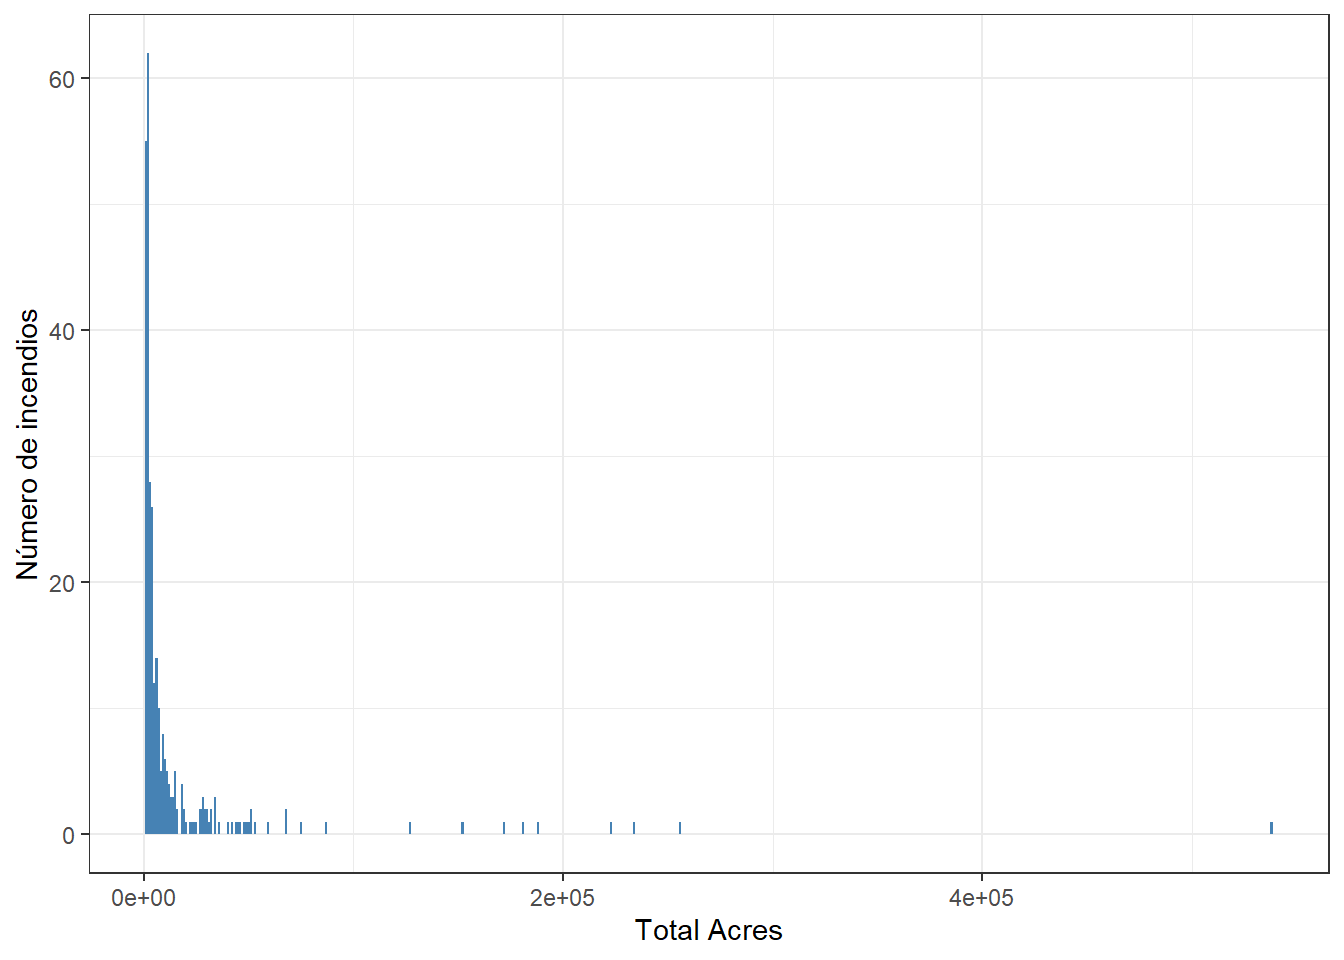
\includegraphics[keepaspectratio]{bookdown-demo_files/figure-latex/hist_vizest-1.pdf}}

{} Ejercicio para entregar

Reconstruya el histograma utilizando un tamaño de celda de 5000. ¿Cuál es el efecto en la salida?

\section{Visualización de la covariación con gráficos de caja}\label{visualizaciuxf3n-de-la-covariaciuxf3n-con-gruxe1ficos-de-caja}

Los gráficos de caja proporcionan una representación visual de la dispersión de los datos de una variable. Estos gráficos muestran el rango de valores de una variable junto con la mediana y los cuartiles. Siga las instrucciones proporcionadas a continuación para crear un gráfico de caja que mide la covariación entre la organización y la superficie total quemada.

Seguimos con los datos de incendios forestales:

\section{Visualización de la covariación con el gráfico de burbuja}\label{visualizaciuxf3n-de-la-covariaciuxf3n-con-el-gruxe1fico-de-burbuja}

La función \texttt{geom\_count()} puede utilizarse con \texttt{ggplot()} para medir la covariación entre variables utilizando diferentes tamaños de símbolos. Siga las instrucciones proporcionadas a continuación para medir la covariación entre la organización y la causa del incendio forestal utilizando el tamaño del símbolo.

Seguimos con los datos de incendios forestales:

\begin{itemize}
\tightlist
\item
  Extraiga el marco de datos y filtre las filas para que sólo se incluyan los \textbf{incendios de entre 5000 y 10000 acres}. A continuación, agrupe los datos por organización. La columna ORGANIZATI del conjunto de datos contiene datos categóricos de los \textbf{organismos del gobierno federal de EE.UU.} que han tenido tierras afectadas por incendios forestales. Por último utilice \texttt{ggplot()} con \texttt{geom\_boxplot()} para crear un \texttt{boxplot} que muestre la distribución de incendios forestales por organización
\end{itemize}

\begin{Shaded}
\begin{Highlighting}[]
\NormalTok{df }\SpecialCharTok{\%\textgreater{}\%}
  \FunctionTok{filter}\NormalTok{(TOTALACRES }\SpecialCharTok{\textgreater{}=} \DecValTok{5000} \SpecialCharTok{\&}\NormalTok{ TOTALACRES }\SpecialCharTok{\textless{}=} \DecValTok{10000}\NormalTok{) }\SpecialCharTok{\%\textgreater{}\%}
  \FunctionTok{group\_by}\NormalTok{(ORGANIZATI) }\SpecialCharTok{\%\textgreater{}\%}
  \FunctionTok{ggplot}\NormalTok{(}\FunctionTok{aes}\NormalTok{(}\AttributeTok{x =}\NormalTok{ ORGANIZATI, }\AttributeTok{y =}\NormalTok{ TOTALACRES)) }\SpecialCharTok{+}
  \FunctionTok{geom\_boxplot}\NormalTok{(}\AttributeTok{fill =} \StringTok{"steelblue"}\NormalTok{, }\AttributeTok{alpha =} \FloatTok{0.7}\NormalTok{, }\AttributeTok{color =} \StringTok{"black"}\NormalTok{) }\SpecialCharTok{+}
  \FunctionTok{stat\_summary}\NormalTok{(}\AttributeTok{fun =}\NormalTok{ mean, }\AttributeTok{geom =} \StringTok{"point"}\NormalTok{, }\AttributeTok{shape =} \DecValTok{20}\NormalTok{, }\AttributeTok{size =} \DecValTok{4}\NormalTok{, }\AttributeTok{color =} \StringTok{"red"}\NormalTok{) }\SpecialCharTok{+}
  \FunctionTok{labs}\NormalTok{(}
    \AttributeTok{x =} \StringTok{"Organización"}\NormalTok{,}
    \AttributeTok{y =} \StringTok{"Total acres"}\NormalTok{,}
    \AttributeTok{title =} \StringTok{"Distribución de acres totales por organización"}
\NormalTok{  ) }\SpecialCharTok{+}
  \FunctionTok{theme\_bw}\NormalTok{()}
\end{Highlighting}
\end{Shaded}

\pandocbounded{\includegraphics[keepaspectratio]{bookdown-demo_files/figure-latex/cajas_vizest-1.pdf}}

{} Ejercicio para entregar

Puede crear también un nuevo \texttt{boxplot} que mapee la covariación de \texttt{CAUSE} y \texttt{TOTALACRES}

\begin{itemize}
\tightlist
\item
  Extraiga el marco de datos y filtre las filas para que sólo se incluyan los \textbf{incendios forestales que se originaron por causas naturales o humanas}. Esto eliminará cualquier registro que son desconocidos o tienen valores perdidos. A continuación, utilice \texttt{geom\_count()} para crear un \textbf{gráfico de símbolos graduados basado en el número de incendios por organización}.
\end{itemize}

\begin{Shaded}
\begin{Highlighting}[]
\NormalTok{df }\SpecialCharTok{\%\textgreater{}\%}
  \FunctionTok{filter}\NormalTok{(CAUSE }\SpecialCharTok{\%in\%} \FunctionTok{c}\NormalTok{(}\StringTok{"Natural"}\NormalTok{, }\StringTok{"Human"}\NormalTok{)) }\SpecialCharTok{\%\textgreater{}\%}
  \FunctionTok{ggplot}\NormalTok{(}\FunctionTok{aes}\NormalTok{(}\AttributeTok{x =}\NormalTok{ ORGANIZATI, }\AttributeTok{y =}\NormalTok{ CAUSE)) }\SpecialCharTok{+}
  \FunctionTok{geom\_count}\NormalTok{(}\FunctionTok{aes}\NormalTok{(}\AttributeTok{color =}\NormalTok{ CAUSE), }\AttributeTok{show.legend =} \ConstantTok{TRUE}\NormalTok{) }\SpecialCharTok{+}
  \FunctionTok{scale\_color\_manual}\NormalTok{(}\AttributeTok{values =} \FunctionTok{c}\NormalTok{(}\StringTok{"Natural"} \OtherTok{=} \StringTok{"\#1b9e77"}\NormalTok{, }\StringTok{"Human"} \OtherTok{=} \StringTok{"\#d95f02"}\NormalTok{)) }\SpecialCharTok{+}
  \FunctionTok{labs}\NormalTok{(}\AttributeTok{x =} \StringTok{"Organización"}\NormalTok{,}
       \AttributeTok{y =} \StringTok{"Causa"}\NormalTok{,}
       \AttributeTok{color =} \StringTok{"Causa"}\NormalTok{,}
       \AttributeTok{size =} \StringTok{"Frecuencia"}\NormalTok{,}
       \AttributeTok{title =} \StringTok{"Incendios por organización y causa"}\NormalTok{) }\SpecialCharTok{+}
  \FunctionTok{theme\_bw}\NormalTok{()}
\end{Highlighting}
\end{Shaded}

\pandocbounded{\includegraphics[keepaspectratio]{bookdown-demo_files/figure-latex/burbuja_vizest-1.pdf}}

\begin{itemize}
\tightlist
\item
  También puede obtener un recuento exacto del número de incendios por organización y causa
\end{itemize}

\begin{Shaded}
\begin{Highlighting}[]
\NormalTok{df }\SpecialCharTok{\%\textgreater{}\%}
  \FunctionTok{count}\NormalTok{(ORGANIZATI, CAUSE)}
\end{Highlighting}
\end{Shaded}

\begin{verbatim}
## # A tibble: 11 x 3
##    ORGANIZATI CAUSE            n
##    <chr>      <chr>        <int>
##  1 BIA        Human           49
##  2 BIA        Natural         91
##  3 BLM        Human          187
##  4 BLM        Natural        386
##  5 FS         Human          158
##  6 FS         Natural        431
##  7 FWS        Human           10
##  8 FWS        Natural          7
##  9 FWS        Undetermined     6
## 10 NPS        Human            6
## 11 NPS        Natural         46
\end{verbatim}

\section{Visualización 2D de contenedores y hexágonos}\label{visualizaciuxf3n-2d-de-contenedores-y-hexuxe1gonos}

También puede utilizar gráficos 2D de contenedores y hexadecimales como una forma alternativa de ver la distribución de dos variables. Siga las instrucciones que se proporcionan a continuación para crear gráficos 2D de cubos y hexágonos que visualicen la relación entre el año y la superficie total quemada

\begin{itemize}
\tightlist
\item
  Utilice la función \texttt{read\_csv()} para cargar el conjunto de datos en un marco de datos
\end{itemize}

\begin{Shaded}
\begin{Highlighting}[]
\NormalTok{df }\OtherTok{\textless{}{-}} \FunctionTok{read\_csv}\NormalTok{(}\StringTok{"data/StudyArea.csv"}\NormalTok{)}
\end{Highlighting}
\end{Shaded}

\begin{itemize}
\tightlist
\item
  Cree un mapa 2D con \texttt{YEAR\_} en el eje \(x\) y \texttt{TOTALACRES} en el eje \(y\)
\end{itemize}

\begin{Shaded}
\begin{Highlighting}[]
\NormalTok{df }\SpecialCharTok{\%\textgreater{}\%} 
  \FunctionTok{ggplot}\NormalTok{(}\FunctionTok{aes}\NormalTok{(}\AttributeTok{x =}\NormalTok{ YEAR\_, }\AttributeTok{y =}\NormalTok{ TOTALACRES)) }\SpecialCharTok{+} 
  \FunctionTok{geom\_bin2d}\NormalTok{(}\AttributeTok{bins =} \DecValTok{40}\NormalTok{) }\SpecialCharTok{+} 
  \FunctionTok{scale\_fill\_viridis\_c}\NormalTok{(}\AttributeTok{option =} \StringTok{"plasma"}\NormalTok{, }\AttributeTok{name =} \StringTok{"Frecuencia"}\NormalTok{) }\SpecialCharTok{+}
  \FunctionTok{labs}\NormalTok{(}
    \AttributeTok{x =} \StringTok{"Year"}\NormalTok{,}
    \AttributeTok{y =} \StringTok{"Total Acres"}\NormalTok{,}
    \AttributeTok{title =} \StringTok{"Distribución conjunta de Year y Total Acres"}\NormalTok{,}
    \AttributeTok{subtitle =} \StringTok{"Mapa de calor con binning en 2D"}
\NormalTok{  ) }\SpecialCharTok{+}
  \FunctionTok{theme\_bw}\NormalTok{()}
\end{Highlighting}
\end{Shaded}

\pandocbounded{\includegraphics[keepaspectratio]{bookdown-demo_files/figure-latex/2d_vizest-1.pdf}}

El gráfico muestra la distribución conjunta de los años (\texttt{YEAR\_}) y el número total de acres (\texttt{TOTALACRES}) mediante un mapa de calor con binning en dos dimensiones. Se observa que la mayor concentración de registros se encuentra en valores bajos de acres (menores a 100.000), lo que indica que la mayoría de las observaciones corresponden a superficies relativamente pequeñas. A su vez, existen pocos casos con valores muy altos (entre 300.000 y más de 600.000 acres), los cuales aparecen como rectángulos aislados y de baja frecuencia, reflejando la presencia de outliers. Finalmente, la acumulación de registros en casi todos los años sugiere un patrón consistente en el tiempo, con algunos picos más notorios después del año 2000.

\section{Visualización de estadísticas ( resumen de los datos)}\label{visualizaciuxf3n-de-estaduxedsticas-resumen-de-los-datos}

Otra técnica básica para realizar un análisis exploratorio de datos es generar varias estadísticas de resumen sobre un conjunto de datos. \textbf{R} incluye una serie de funciones individuales para generar estadísticas de resumen específicas o puede utilizar la función summarise() para generar un conjunto de estadísticas de resumen

\begin{itemize}
\tightlist
\item
  Carguemos nuevamente la data de incendios forestales
\end{itemize}

\begin{Shaded}
\begin{Highlighting}[]
\NormalTok{datos }\OtherTok{\textless{}{-}} \FunctionTok{read\_csv}\NormalTok{(}\StringTok{"data/StudyArea.csv"}\NormalTok{)}
\end{Highlighting}
\end{Shaded}

\begin{itemize}
\tightlist
\item
  Restringir la lista de columnas y filtra la lista para incluir sólo los incendios forestales de más de 1000 acres
\end{itemize}

\begin{Shaded}
\begin{Highlighting}[]
\NormalTok{df }\OtherTok{\textless{}{-}}\NormalTok{ datos }\SpecialCharTok{\%\textgreater{}\%}
  \FunctionTok{select}\NormalTok{(ORGANIZATI, STATE, YEAR\_, TOTALACRES, CAUSE) }\SpecialCharTok{\%\textgreater{}\%} 
  \FunctionTok{filter}\NormalTok{(TOTALACRES }\SpecialCharTok{\textgreater{}=} \DecValTok{1000}\NormalTok{)}
\end{Highlighting}
\end{Shaded}

\begin{itemize}
\tightlist
\item
  Hagamos un resumen estadístico de la columna TOTALACRES
\end{itemize}

\begin{Shaded}
\begin{Highlighting}[]
\NormalTok{df }\SpecialCharTok{\%\textgreater{}\%} 
  \FunctionTok{summarise}\NormalTok{(}\AttributeTok{n =} \FunctionTok{length}\NormalTok{(TOTALACRES),}
            \AttributeTok{media =} \FunctionTok{mean}\NormalTok{(TOTALACRES),}
            \AttributeTok{ds =} \FunctionTok{sd}\NormalTok{(TOTALACRES),}
            \AttributeTok{mediana =} \FunctionTok{median}\NormalTok{(TOTALACRES),}
            \AttributeTok{q1 =} \FunctionTok{quantile}\NormalTok{(TOTALACRES)[}\DecValTok{2}\NormalTok{],}
            \AttributeTok{q3 =} \FunctionTok{quantile}\NormalTok{(TOTALACRES)[}\DecValTok{4}\NormalTok{],}
            \AttributeTok{RIC =} \FunctionTok{IQR}\NormalTok{(TOTALACRES),}
            \AttributeTok{minimo =} \FunctionTok{min}\NormalTok{(TOTALACRES),}
            \AttributeTok{maximo =} \FunctionTok{max}\NormalTok{(TOTALACRES)) }\OtherTok{{-}\textgreater{}}\NormalTok{ resumen\_totalacres}
\end{Highlighting}
\end{Shaded}

El análisis se realizó sobre \textbf{7288 registros}, con un valor promedio cercano a \textbf{10813} y una gran variabilidad, dado que la desviación estándar es de aproximadamente \textbf{28579}. El \textbf{50\% de los datos} se encuentra en torno a \textbf{3240}, lo que indica que la mitad de las observaciones están por debajo de ese valor. El \textbf{25\% más bajo} de los registros toma valores hasta \textbf{1670}, mientras que el \textbf{25\% más alto} supera los \textbf{8283}. El rango intermedio entre el 25\% inferior y el 75\% superior es de aproximadamente \textbf{6613}, reflejando una fuerte dispersión en los datos. Finalmente, los valores observados van desde un mínimo de \textbf{1000} hasta un máximo de \textbf{590620}, lo que muestra la presencia de valores extremos mucho más altos que la mayoría de las observaciones.

\section{Visualización de un gráfico de correlación}\label{visualizaciuxf3n-de-un-gruxe1fico-de-correlaciuxf3n}

Es una representación gráfica de una matriz de correlaciones entre varias variables numéricas.

\begin{itemize}
\item
  Se muestran en forma de mapa de calor (heatmap), círculos, o elipses que varían en tamaño y color según la intensidad y signo de la correlación.
\item
  Su objetivo es facilitar la identificación de relaciones lineales fuertes, tanto positivas como negativas, entre todas las variables del conjunto de datos.
\item
  Carguemos los datos de la banca
\end{itemize}

\begin{Shaded}
\begin{Highlighting}[]
\NormalTok{bank }\OtherTok{\textless{}{-}} \FunctionTok{read\_delim}\NormalTok{(}\StringTok{"https://raw.githubusercontent.com/cdeoroaguado/Datos/refs/heads/main/datamanip/bank/bank.csv"}\NormalTok{,}\AttributeTok{delim =} \StringTok{";"}\NormalTok{,}\AttributeTok{quote =} \StringTok{"}\SpecialCharTok{\textbackslash{}"}\StringTok{"}\NormalTok{)}

\FunctionTok{head}\NormalTok{(bank,}\AttributeTok{n=}\DecValTok{5}\NormalTok{)}
\end{Highlighting}
\end{Shaded}

\begin{verbatim}
## # A tibble: 5 x 17
##     age job   marital education default balance housing loan  contact
##   <dbl> <chr> <chr>   <chr>     <chr>     <dbl> <chr>   <chr> <chr>  
## 1    30 unem~ married primary   no         1787 no      no    cellul~
## 2    33 serv~ married secondary no         4789 yes     yes   cellul~
## 3    35 mana~ single  tertiary  no         1350 yes     no    cellul~
## 4    30 mana~ married tertiary  no         1476 yes     yes   unknown
## 5    59 blue~ married secondary no            0 yes     no    unknown
## # i 8 more variables: day <dbl>, month <chr>, duration <dbl>,
## #   campaign <dbl>, pdays <dbl>, previous <dbl>, poutcome <chr>,
## #   y <chr>
\end{verbatim}

\begin{itemize}
\tightlist
\item
  Selecciona las variables numéricas
\end{itemize}

\begin{Shaded}
\begin{Highlighting}[]
\CommentTok{\# Seleccionar las variables numéricas}
\NormalTok{num\_vars }\OtherTok{\textless{}{-}}\NormalTok{ bank }\SpecialCharTok{\%\textgreater{}\%} 
  \FunctionTok{select}\NormalTok{(age, balance, duration)}
\end{Highlighting}
\end{Shaded}

\begin{itemize}
\tightlist
\item
  Hagamos la matriz de correlación y el gráfico \texttt{heatmap} con las variables numéricas
\end{itemize}

\begin{Shaded}
\begin{Highlighting}[]
\CommentTok{\# libreria}
\FunctionTok{library}\NormalTok{(corrplot)}

\CommentTok{\# Calcular matriz de correlación}
\NormalTok{matriz\_cor }\OtherTok{\textless{}{-}} \FunctionTok{cor}\NormalTok{(num\_vars, }\AttributeTok{use =} \StringTok{"complete.obs"}\NormalTok{)}

\FunctionTok{print}\NormalTok{(matriz\_cor)}
\end{Highlighting}
\end{Shaded}

\begin{verbatim}
##                   age     balance     duration
## age       1.000000000  0.08382014 -0.002366889
## balance   0.083820142  1.00000000 -0.015949918
## duration -0.002366889 -0.01594992  1.000000000
\end{verbatim}

\begin{Shaded}
\begin{Highlighting}[]
\CommentTok{\# Heatmap }
\FunctionTok{corrplot}\NormalTok{(matriz\_cor, }\AttributeTok{method=}\StringTok{"number"}\NormalTok{)}
\end{Highlighting}
\end{Shaded}

\pandocbounded{\includegraphics[keepaspectratio]{bookdown-demo_files/figure-latex/corr_est_vizest-1.pdf}}

Vemos que no hay correlación entre ellos.

\section{Visualización de un gráfico de dispersión}\label{visualizaciuxf3n-de-un-gruxe1fico-de-dispersiuxf3n}

Un diagrama de dispersión es un gráfico en el que los valores de dos variables se trazan a lo largo de dos ejes, y el patrón de los puntos resultantes revela cualquier correlación presente

\begin{itemize}
\tightlist
\item
  Cargar el contenido del archivo \texttt{StudyArea.csv} en un marco de datos
\end{itemize}

\begin{Shaded}
\begin{Highlighting}[]
\NormalTok{df }\OtherTok{\textless{}{-}} \FunctionTok{read\_csv}\NormalTok{(}\StringTok{"data/StudyArea.csv"}\NormalTok{)}
\end{Highlighting}
\end{Shaded}

\begin{itemize}
\tightlist
\item
  Utilice \texttt{ggplot()} para crear un gráfico de dispersión con el año en el eje \(x\) y el total de acres quemados en el eje \(y\).
\end{itemize}

\begin{Shaded}
\begin{Highlighting}[]
\NormalTok{df }\SpecialCharTok{\%\textgreater{}\%} 
  \FunctionTok{select}\NormalTok{(ORGANIZATI, YEAR\_, TOTALACRES) }\SpecialCharTok{\%\textgreater{}\%} 
  \FunctionTok{group\_by}\NormalTok{(YEAR\_) }\SpecialCharTok{\%\textgreater{}\%} 
  \FunctionTok{summarise}\NormalTok{(}\AttributeTok{totalacres =} \FunctionTok{sum}\NormalTok{(TOTALACRES, }\AttributeTok{na.rm =} \ConstantTok{TRUE}\NormalTok{)) }\SpecialCharTok{\%\textgreater{}\%} 
  \FunctionTok{ggplot}\NormalTok{(}\FunctionTok{aes}\NormalTok{(}\AttributeTok{x =}\NormalTok{ YEAR\_, }\AttributeTok{y =}\NormalTok{ totalacres)) }\SpecialCharTok{+}
  \FunctionTok{geom\_point}\NormalTok{(}\AttributeTok{color =} \StringTok{"darkred"}\NormalTok{, }\AttributeTok{size =} \DecValTok{3}\NormalTok{) }\SpecialCharTok{+}             
  \FunctionTok{labs}\NormalTok{(}\AttributeTok{title =} \StringTok{"Evolución de Total Acres por Año"}\NormalTok{,}
       \AttributeTok{x =} \StringTok{"Año"}\NormalTok{,}
       \AttributeTok{y =} \StringTok{"Total Acres"}\NormalTok{) }\SpecialCharTok{+}
  \FunctionTok{theme\_bw}\NormalTok{()}
\end{Highlighting}
\end{Shaded}

\pandocbounded{\includegraphics[keepaspectratio]{bookdown-demo_files/figure-latex/dispersion1_vizest-1.pdf}}

\begin{itemize}
\tightlist
\item
  Hay ocasiones en las que tiene sentido utilizar las escalas logarítmicas en los cuadros y gráficos. Una de las razones es responder a la asimetría hacia los valores grandes, es decir, los casos en los que uno o unos pocos puntos son mucho más grandes que el grueso de los datos. En el gráfico que acabamos de crear hay un par de puntos que entran en esta categoría en en el eje Y. Vuelva a crear el gráfico, pero esta vez utilice la función \texttt{log()} en la columna totalacres
\end{itemize}

\begin{Shaded}
\begin{Highlighting}[]
\NormalTok{df }\SpecialCharTok{\%\textgreater{}\%} 
  \FunctionTok{select}\NormalTok{(ORGANIZATI, YEAR\_, TOTALACRES) }\SpecialCharTok{\%\textgreater{}\%} 
  \FunctionTok{group\_by}\NormalTok{(YEAR\_) }\SpecialCharTok{\%\textgreater{}\%} 
  \FunctionTok{summarise}\NormalTok{(}\AttributeTok{totalacres =} \FunctionTok{sum}\NormalTok{(TOTALACRES, }\AttributeTok{na.rm =} \ConstantTok{TRUE}\NormalTok{)) }\SpecialCharTok{\%\textgreater{}\%} 
  \FunctionTok{ggplot}\NormalTok{(}\FunctionTok{aes}\NormalTok{(}\AttributeTok{x =}\NormalTok{ YEAR\_, }\AttributeTok{y =} \FunctionTok{log}\NormalTok{(totalacres))) }\SpecialCharTok{+}
  \FunctionTok{geom\_point}\NormalTok{(}\AttributeTok{color =} \StringTok{"darkred"}\NormalTok{, }\AttributeTok{size =} \DecValTok{3}\NormalTok{) }\SpecialCharTok{+}             
  \FunctionTok{labs}\NormalTok{(}\AttributeTok{title =} \StringTok{"Evolución de Total Acres por Año"}\NormalTok{,}
       \AttributeTok{x =} \StringTok{"Año"}\NormalTok{,}
       \AttributeTok{y =} \StringTok{"Total Acres"}\NormalTok{) }\SpecialCharTok{+}
  \FunctionTok{theme\_bw}\NormalTok{()}
\end{Highlighting}
\end{Shaded}

\pandocbounded{\includegraphics[keepaspectratio]{bookdown-demo_files/figure-latex/dispersion1log_vizest-1.pdf}}

\section{Visualización del gráfico de dispersión con linea de tendencia}\label{visualizaciuxf3n-del-gruxe1fico-de-dispersiuxf3n-con-linea-de-tendencia}

Los gráficos construidos con \texttt{ggplot()} pueden tener más de una geometría. Es habitual añadir una línea de predicción (regresión) al gráfico.

Hay varias maneras de añadir una línea de regresión al gráfico de dispersión, una de ellas es utilizar la función \texttt{geom\_smooth()}

\begin{itemize}
\tightlist
\item
  Regresion con \texttt{method\ =\ lm}
\end{itemize}

\begin{Shaded}
\begin{Highlighting}[]
\NormalTok{df }\SpecialCharTok{\%\textgreater{}\%} 
  \FunctionTok{select}\NormalTok{(ORGANIZATI, YEAR\_, TOTALACRES) }\SpecialCharTok{\%\textgreater{}\%} 
  \FunctionTok{group\_by}\NormalTok{(YEAR\_) }\SpecialCharTok{\%\textgreater{}\%} 
  \FunctionTok{summarise}\NormalTok{(}\AttributeTok{totalacres =} \FunctionTok{sum}\NormalTok{(TOTALACRES, }\AttributeTok{na.rm =} \ConstantTok{TRUE}\NormalTok{)) }\SpecialCharTok{\%\textgreater{}\%} 
  \FunctionTok{ggplot}\NormalTok{(}\FunctionTok{aes}\NormalTok{(}\AttributeTok{x =}\NormalTok{ YEAR\_, }\AttributeTok{y =} \FunctionTok{log}\NormalTok{(totalacres))) }\SpecialCharTok{+}
  \FunctionTok{geom\_point}\NormalTok{(}\AttributeTok{color =} \StringTok{"darkred"}\NormalTok{, }\AttributeTok{size =} \DecValTok{3}\NormalTok{) }\SpecialCharTok{+}
  \FunctionTok{geom\_smooth}\NormalTok{(}\AttributeTok{method=}\NormalTok{lm, }\AttributeTok{se=}\ConstantTok{FALSE}\NormalTok{)}\SpecialCharTok{+}
  \FunctionTok{labs}\NormalTok{(}\AttributeTok{title =} \StringTok{"Evolución de Total Acres por Año"}\NormalTok{,}
       \AttributeTok{x =} \StringTok{"Año"}\NormalTok{,}
       \AttributeTok{y =} \StringTok{"Total Acres"}\NormalTok{) }\SpecialCharTok{+}
  \FunctionTok{theme\_bw}\NormalTok{()}
\end{Highlighting}
\end{Shaded}

\pandocbounded{\includegraphics[keepaspectratio]{bookdown-demo_files/figure-latex/smoo_vizest-1.pdf}}

\begin{itemize}
\tightlist
\item
  Regresion con \texttt{method\ =\ loess}
\end{itemize}

\begin{Shaded}
\begin{Highlighting}[]
\NormalTok{df }\SpecialCharTok{\%\textgreater{}\%} 
  \FunctionTok{select}\NormalTok{(ORGANIZATI, YEAR\_, TOTALACRES) }\SpecialCharTok{\%\textgreater{}\%} 
  \FunctionTok{group\_by}\NormalTok{(YEAR\_) }\SpecialCharTok{\%\textgreater{}\%} 
  \FunctionTok{summarise}\NormalTok{(}\AttributeTok{totalacres =} \FunctionTok{sum}\NormalTok{(TOTALACRES, }\AttributeTok{na.rm =} \ConstantTok{TRUE}\NormalTok{)) }\SpecialCharTok{\%\textgreater{}\%} 
  \FunctionTok{ggplot}\NormalTok{(}\FunctionTok{aes}\NormalTok{(}\AttributeTok{x =}\NormalTok{ YEAR\_, }\AttributeTok{y =} \FunctionTok{log}\NormalTok{(totalacres))) }\SpecialCharTok{+}
  \FunctionTok{geom\_point}\NormalTok{(}\AttributeTok{color =} \StringTok{"darkred"}\NormalTok{, }\AttributeTok{size =} \DecValTok{3}\NormalTok{) }\SpecialCharTok{+}
  \FunctionTok{geom\_smooth}\NormalTok{(}\AttributeTok{method =} \StringTok{"loess"}\NormalTok{, }\AttributeTok{se=}\ConstantTok{FALSE}\NormalTok{)}\SpecialCharTok{+}
  \FunctionTok{labs}\NormalTok{(}\AttributeTok{title =} \StringTok{"Evolución de Total Acres por Año"}\NormalTok{,}
       \AttributeTok{x =} \StringTok{"Año"}\NormalTok{,}
       \AttributeTok{y =} \StringTok{"Total Acres"}\NormalTok{) }\SpecialCharTok{+}
  \FunctionTok{theme\_bw}\NormalTok{()}
\end{Highlighting}
\end{Shaded}

\pandocbounded{\includegraphics[keepaspectratio]{bookdown-demo_files/figure-latex/smoot_vizest-1.pdf}}

\begin{itemize}
\tightlist
\item
  Regresion con \texttt{method\ =\ loess} con intervalo de confianza
\end{itemize}

\begin{Shaded}
\begin{Highlighting}[]
\NormalTok{df }\SpecialCharTok{\%\textgreater{}\%} 
  \FunctionTok{select}\NormalTok{(ORGANIZATI, YEAR\_, TOTALACRES) }\SpecialCharTok{\%\textgreater{}\%} 
  \FunctionTok{group\_by}\NormalTok{(YEAR\_) }\SpecialCharTok{\%\textgreater{}\%} 
  \FunctionTok{summarise}\NormalTok{(}\AttributeTok{totalacres =} \FunctionTok{sum}\NormalTok{(TOTALACRES, }\AttributeTok{na.rm =} \ConstantTok{TRUE}\NormalTok{)) }\SpecialCharTok{\%\textgreater{}\%} 
  \FunctionTok{ggplot}\NormalTok{(}\FunctionTok{aes}\NormalTok{(}\AttributeTok{x =}\NormalTok{ YEAR\_, }\AttributeTok{y =} \FunctionTok{log}\NormalTok{(totalacres))) }\SpecialCharTok{+}
  \FunctionTok{geom\_point}\NormalTok{(}\AttributeTok{color =} \StringTok{"darkred"}\NormalTok{, }\AttributeTok{size =} \DecValTok{3}\NormalTok{) }\SpecialCharTok{+}
  \FunctionTok{geom\_smooth}\NormalTok{(}\AttributeTok{method =} \StringTok{"loess"}\NormalTok{, }\AttributeTok{se=}\ConstantTok{TRUE}\NormalTok{)}\SpecialCharTok{+}
  \FunctionTok{labs}\NormalTok{(}\AttributeTok{title =} \StringTok{"Evolución de Total Acres por Año"}\NormalTok{,}
       \AttributeTok{x =} \StringTok{"Año"}\NormalTok{,}
       \AttributeTok{y =} \StringTok{"Total Acres"}\NormalTok{) }\SpecialCharTok{+}
  \FunctionTok{theme\_bw}\NormalTok{()}
\end{Highlighting}
\end{Shaded}

\pandocbounded{\includegraphics[keepaspectratio]{bookdown-demo_files/figure-latex/smooth1_vizest-1.pdf}}

\section{Visualización de trazado de categorías}\label{visualizaciuxf3n-de-trazado-de-categoruxedas}

En lugar de representar gráficamente todo el conjunto de incendios forestales, es posible que se quiera comprender mejor las tendencias por estado. En este paso creará un nuevo gráfico de dispersión que visualice las tendencias de los incendios forestales a lo largo del tiempo por estado

\begin{itemize}
\tightlist
\item
  Reagrupar el marco de datos de los incendios forestales por estado y año, despues resuma los grupos por el total de hectáreas quemadas y Añade un parámetro de parámetro de color a la función \texttt{aes()} para que los puntos y la línea de regresión se se mapeen de acuerdo con el estado en el que se produjeron
\end{itemize}

\begin{Shaded}
\begin{Highlighting}[]
\NormalTok{df }\SpecialCharTok{\%\textgreater{}\%} 
  \FunctionTok{group\_by}\NormalTok{(STATE, YEAR\_) }\SpecialCharTok{\%\textgreater{}\%} 
  \FunctionTok{summarise}\NormalTok{(}\AttributeTok{totalacres =} \FunctionTok{sum}\NormalTok{(TOTALACRES)) }\SpecialCharTok{\%\textgreater{}\%} 
  \FunctionTok{ggplot}\NormalTok{(}\FunctionTok{aes}\NormalTok{(}\AttributeTok{x=}\NormalTok{YEAR\_, }\AttributeTok{y=}\NormalTok{totalacres, }\AttributeTok{colour=}\NormalTok{STATE)) }\SpecialCharTok{+} 
  \FunctionTok{geom\_point}\NormalTok{(}\FunctionTok{aes}\NormalTok{(}\AttributeTok{colour =}\NormalTok{ STATE)) }\SpecialCharTok{+} 
  \FunctionTok{stat\_smooth}\NormalTok{(}\AttributeTok{method=}\NormalTok{lm, }\AttributeTok{se=}\ConstantTok{FALSE}\NormalTok{)}\SpecialCharTok{+}
  \FunctionTok{theme\_bw}\NormalTok{()}
\end{Highlighting}
\end{Shaded}

\pandocbounded{\includegraphics[keepaspectratio]{bookdown-demo_files/figure-latex/smo_vizest-1.pdf}}

\section{Visualizacion etiquetando nombres}\label{visualizacion-etiquetando-nombres}

Puede añadir etiquetas a su gráfico mediante la función \texttt{geom\_text()} o la función \texttt{geom\_\ label()}

\begin{Shaded}
\begin{Highlighting}[]
\NormalTok{df }\SpecialCharTok{\%\textgreater{}\%} 
  \FunctionTok{group\_by}\NormalTok{(STATE, YEAR\_) }\SpecialCharTok{\%\textgreater{}\%} 
  \FunctionTok{summarise}\NormalTok{(}\AttributeTok{totalacres =} \FunctionTok{sum}\NormalTok{(TOTALACRES)) }\SpecialCharTok{\%\textgreater{}\%} 
  \FunctionTok{ggplot}\NormalTok{(}\FunctionTok{aes}\NormalTok{(}\AttributeTok{x=}\NormalTok{YEAR\_, }\AttributeTok{y=}\FunctionTok{log}\NormalTok{(totalacres))) }\SpecialCharTok{+} 
  \FunctionTok{geom\_point}\NormalTok{() }\SpecialCharTok{+}
  \FunctionTok{geom\_smooth}\NormalTok{(}\AttributeTok{method=}\NormalTok{loess, }\AttributeTok{se=}\ConstantTok{TRUE}\NormalTok{) }\SpecialCharTok{+} 
  \FunctionTok{geom\_text}\NormalTok{(}\FunctionTok{aes}\NormalTok{(}\AttributeTok{label=}\NormalTok{STATE), }\AttributeTok{size=}\DecValTok{3}\NormalTok{)}\SpecialCharTok{+}
  \FunctionTok{theme\_bw}\NormalTok{()}
\end{Highlighting}
\end{Shaded}

\pandocbounded{\includegraphics[keepaspectratio]{bookdown-demo_files/figure-latex/etiq_vizest-1.pdf}}
La pantalla está extremadamente desordenada así que vamos a ajustar algunos parámetros para hacer esto más fácil de leer.

\begin{itemize}
\tightlist
\item
  Puede utilizar el parámetro \texttt{check\_overlap} para eliminar cualquier etiqueta superpuesta. Actualice su código como se ve a continuación
\end{itemize}

\begin{Shaded}
\begin{Highlighting}[]
\NormalTok{df }\SpecialCharTok{\%\textgreater{}\%} 
  \FunctionTok{group\_by}\NormalTok{(STATE, YEAR\_) }\SpecialCharTok{\%\textgreater{}\%} 
  \FunctionTok{summarise}\NormalTok{(}\AttributeTok{totalacres =} \FunctionTok{sum}\NormalTok{(TOTALACRES)) }\SpecialCharTok{\%\textgreater{}\%} 
  \FunctionTok{ggplot}\NormalTok{(}\FunctionTok{aes}\NormalTok{(}\AttributeTok{x=}\NormalTok{YEAR\_, }\AttributeTok{y=}\FunctionTok{log}\NormalTok{(totalacres))) }\SpecialCharTok{+} 
  \FunctionTok{geom\_point}\NormalTok{() }\SpecialCharTok{+}
  \FunctionTok{geom\_smooth}\NormalTok{(}\AttributeTok{method=}\NormalTok{loess, }\AttributeTok{se=}\ConstantTok{TRUE}\NormalTok{) }\SpecialCharTok{+} 
  \FunctionTok{geom\_text}\NormalTok{(}\FunctionTok{aes}\NormalTok{(}\AttributeTok{label=}\NormalTok{STATE), }\AttributeTok{size=}\DecValTok{3}\NormalTok{, }\AttributeTok{check\_overlap =} \ConstantTok{TRUE}\NormalTok{)}\SpecialCharTok{+}
  \FunctionTok{theme\_bw}\NormalTok{()}
\end{Highlighting}
\end{Shaded}

\pandocbounded{\includegraphics[keepaspectratio]{bookdown-demo_files/figure-latex/etiq2_vizest-1.pdf}}

\begin{itemize}
\tightlist
\item
  Esto se ve un poco mejor, pero si se cambia el tamaño de la etiqueta a 2 se reducirá aún más reducir el desorden y la superposición, mientras que esperamos que siga siendo legible. Habrás observado que las etiquetas se sitúan directamente sobre los temas. Puede utilizar los parámetros \texttt{nudge\_x} y \texttt{nudge\_y} para mover las etiquetas en relación con el punto. Utilice \texttt{nudge\_x} como se ve a continuación para ver cómo esto mueve las etiquetas horizontalmente
\end{itemize}

\begin{Shaded}
\begin{Highlighting}[]
\NormalTok{df }\SpecialCharTok{\%\textgreater{}\%} 
  \FunctionTok{group\_by}\NormalTok{(STATE, YEAR\_) }\SpecialCharTok{\%\textgreater{}\%} 
  \FunctionTok{summarise}\NormalTok{(}\AttributeTok{totalacres =} \FunctionTok{sum}\NormalTok{(TOTALACRES)) }\SpecialCharTok{\%\textgreater{}\%} 
  \FunctionTok{ggplot}\NormalTok{(}\FunctionTok{aes}\NormalTok{(}\AttributeTok{x=}\NormalTok{YEAR\_, }\AttributeTok{y=}\FunctionTok{log}\NormalTok{(totalacres))) }\SpecialCharTok{+} 
  \FunctionTok{geom\_point}\NormalTok{() }\SpecialCharTok{+}
  \FunctionTok{geom\_smooth}\NormalTok{(}\AttributeTok{method=}\NormalTok{loess, }\AttributeTok{se=}\ConstantTok{TRUE}\NormalTok{) }\SpecialCharTok{+} 
  \FunctionTok{geom\_text}\NormalTok{(}\FunctionTok{aes}\NormalTok{(}\AttributeTok{label=}\NormalTok{STATE), }\AttributeTok{size=}\DecValTok{3}\NormalTok{, }\AttributeTok{check\_overlap =} \ConstantTok{TRUE}\NormalTok{,}\AttributeTok{nudge\_x =} \FloatTok{1.0}\NormalTok{)}\SpecialCharTok{+}
  \FunctionTok{theme\_bw}\NormalTok{()}
\end{Highlighting}
\end{Shaded}

\pandocbounded{\includegraphics[keepaspectratio]{bookdown-demo_files/figure-latex/etiq3_vizest-1.pdf}}

\begin{itemize}
\tightlist
\item
  También puede colorear las etiquetas por categoría añadiendo el parámetro de color a la función \texttt{aes()} para \texttt{geom\_text()}
\end{itemize}

\begin{Shaded}
\begin{Highlighting}[]
\NormalTok{df }\SpecialCharTok{\%\textgreater{}\%} 
  \FunctionTok{group\_by}\NormalTok{(STATE, YEAR\_) }\SpecialCharTok{\%\textgreater{}\%} 
  \FunctionTok{summarise}\NormalTok{(}\AttributeTok{totalacres =} \FunctionTok{sum}\NormalTok{(TOTALACRES)) }\SpecialCharTok{\%\textgreater{}\%} 
  \FunctionTok{ggplot}\NormalTok{(}\FunctionTok{aes}\NormalTok{(}\AttributeTok{x=}\NormalTok{YEAR\_, }\AttributeTok{y=}\FunctionTok{log}\NormalTok{(totalacres))) }\SpecialCharTok{+} 
  \FunctionTok{geom\_point}\NormalTok{() }\SpecialCharTok{+}
  \FunctionTok{geom\_smooth}\NormalTok{(}\AttributeTok{method=}\NormalTok{loess, }\AttributeTok{se=}\ConstantTok{TRUE}\NormalTok{) }\SpecialCharTok{+} 
  \FunctionTok{geom\_text}\NormalTok{(}\FunctionTok{aes}\NormalTok{(}\AttributeTok{label=}\NormalTok{STATE,}\AttributeTok{color=}\NormalTok{STATE), }\AttributeTok{size=}\DecValTok{3}\NormalTok{, }\AttributeTok{check\_overlap =} \ConstantTok{TRUE}\NormalTok{,}\AttributeTok{nudge\_x =} \FloatTok{1.0}\NormalTok{)}\SpecialCharTok{+}
  \FunctionTok{theme\_bw}\NormalTok{()}
\end{Highlighting}
\end{Shaded}

\pandocbounded{\includegraphics[keepaspectratio]{bookdown-demo_files/figure-latex/etiq4_vizest-1.pdf}}

\begin{itemize}
\tightlist
\item
  También puedes añadir un subtítulo y un pie de foto con el código que ves a continuación
\end{itemize}

\begin{Shaded}
\begin{Highlighting}[]
\NormalTok{df }\SpecialCharTok{\%\textgreater{}\%} 
  \FunctionTok{group\_by}\NormalTok{(STATE, YEAR\_) }\SpecialCharTok{\%\textgreater{}\%} 
  \FunctionTok{summarise}\NormalTok{(}\AttributeTok{totalacres =} \FunctionTok{sum}\NormalTok{(TOTALACRES)) }\SpecialCharTok{\%\textgreater{}\%} 
  \FunctionTok{ggplot}\NormalTok{(}\FunctionTok{aes}\NormalTok{(}\AttributeTok{x=}\NormalTok{YEAR\_, }\AttributeTok{y=}\FunctionTok{log}\NormalTok{(totalacres))) }\SpecialCharTok{+} 
  \FunctionTok{geom\_point}\NormalTok{() }\SpecialCharTok{+}
  \FunctionTok{geom\_smooth}\NormalTok{(}\AttributeTok{method=}\NormalTok{loess, }\AttributeTok{se=}\ConstantTok{TRUE}\NormalTok{) }\SpecialCharTok{+} 
  \FunctionTok{geom\_text}\NormalTok{(}\FunctionTok{aes}\NormalTok{(}\AttributeTok{label=}\NormalTok{STATE,}\AttributeTok{color=}\NormalTok{STATE), }\AttributeTok{size=}\DecValTok{3}\NormalTok{, }\AttributeTok{check\_overlap =} \ConstantTok{TRUE}\NormalTok{,}\AttributeTok{nudge\_x =} \FloatTok{1.0}\NormalTok{)}\SpecialCharTok{+}
  \FunctionTok{theme\_bw}\NormalTok{()}
\end{Highlighting}
\end{Shaded}

\pandocbounded{\includegraphics[keepaspectratio]{bookdown-demo_files/figure-latex/etiq5_vizest-1.pdf}}

\begin{itemize}
\tightlist
\item
  También puedes añadir un subtítulo y un pie de foto con el código que ves a continuación
\end{itemize}

\begin{Shaded}
\begin{Highlighting}[]
\NormalTok{df }\SpecialCharTok{\%\textgreater{}\%} 
  \FunctionTok{group\_by}\NormalTok{(STATE, YEAR\_) }\SpecialCharTok{\%\textgreater{}\%} 
  \FunctionTok{summarise}\NormalTok{(}\AttributeTok{totalacres =} \FunctionTok{sum}\NormalTok{(TOTALACRES)) }\SpecialCharTok{\%\textgreater{}\%} 
  \FunctionTok{ggplot}\NormalTok{(}\FunctionTok{aes}\NormalTok{(}\AttributeTok{x =}\NormalTok{ YEAR\_, }\AttributeTok{y =} \FunctionTok{log}\NormalTok{(totalacres))) }\SpecialCharTok{+} 
  \FunctionTok{geom\_point}\NormalTok{(}\AttributeTok{color =} \StringTok{"steelblue"}\NormalTok{, }\AttributeTok{size =} \DecValTok{2}\NormalTok{, }\AttributeTok{alpha =} \FloatTok{0.7}\NormalTok{) }\SpecialCharTok{+}
  \FunctionTok{geom\_smooth}\NormalTok{(}\AttributeTok{method =} \StringTok{"loess"}\NormalTok{, }\AttributeTok{se =} \ConstantTok{TRUE}\NormalTok{, }\AttributeTok{span =} \FloatTok{0.5}\NormalTok{, }\AttributeTok{color =} \StringTok{"darkorange"}\NormalTok{)}\SpecialCharTok{+}
  \FunctionTok{labs}\NormalTok{(}\AttributeTok{title=}\FunctionTok{paste}\NormalTok{(}\StringTok{"La superficie quemada por incendios forestales las ultimas decadas"}\NormalTok{), }\AttributeTok{subtitle=}\FunctionTok{paste}\NormalTok{(}\StringTok{"1980{-}2016"}\NormalTok{), }\AttributeTok{caption=}\StringTok{"Data from USGS"}\NormalTok{)}\SpecialCharTok{+}
  \FunctionTok{theme\_bw}\NormalTok{()}
\end{Highlighting}
\end{Shaded}

\pandocbounded{\includegraphics[keepaspectratio]{bookdown-demo_files/figure-latex/etiq10_vizest-1.pdf}}

\begin{itemize}
\tightlist
\item
  También puede actualizar las etiquetas X e Y del gráfico. Actualice estas etiquetas en su gráfico usando el código que ve abajo
\end{itemize}

\begin{Shaded}
\begin{Highlighting}[]
\NormalTok{df }\SpecialCharTok{\%\textgreater{}\%} 
  \FunctionTok{group\_by}\NormalTok{(STATE, YEAR\_) }\SpecialCharTok{\%\textgreater{}\%} 
  \FunctionTok{summarise}\NormalTok{(}\AttributeTok{totalacres =} \FunctionTok{sum}\NormalTok{(TOTALACRES)) }\SpecialCharTok{\%\textgreater{}\%} 
  \FunctionTok{ggplot}\NormalTok{(}\FunctionTok{aes}\NormalTok{(}\AttributeTok{x =}\NormalTok{ YEAR\_, }\AttributeTok{y =} \FunctionTok{log}\NormalTok{(totalacres))) }\SpecialCharTok{+} 
  \FunctionTok{geom\_point}\NormalTok{(}\AttributeTok{color =} \StringTok{"steelblue"}\NormalTok{, }\AttributeTok{size =} \DecValTok{2}\NormalTok{, }\AttributeTok{alpha =} \FloatTok{0.7}\NormalTok{) }\SpecialCharTok{+}
  \FunctionTok{geom\_smooth}\NormalTok{(}\AttributeTok{method =} \StringTok{"loess"}\NormalTok{, }\AttributeTok{se =} \ConstantTok{TRUE}\NormalTok{, }\AttributeTok{span =} \FloatTok{0.5}\NormalTok{, }\AttributeTok{color =} \StringTok{"darkorange"}\NormalTok{)}\SpecialCharTok{+}
  \FunctionTok{labs}\NormalTok{(}\AttributeTok{title=}\FunctionTok{paste}\NormalTok{(}\StringTok{"La superficie quemada por incendios forestales las ultimas decadas"}\NormalTok{), }\AttributeTok{subtitle=}\FunctionTok{paste}\NormalTok{(}\StringTok{"1980{-}2016"}\NormalTok{), }\AttributeTok{caption=}\StringTok{"Data from USGS"}\NormalTok{)}\SpecialCharTok{+}
  \FunctionTok{scale\_y\_continuous}\NormalTok{(}\AttributeTok{name=}\StringTok{"Log del total acres quemadas"}\NormalTok{) }\SpecialCharTok{+} 
  \FunctionTok{scale\_x\_continuous}\NormalTok{(}\AttributeTok{name=}\StringTok{"Year quemados"}\NormalTok{)}\SpecialCharTok{+}
  \FunctionTok{theme\_bw}\NormalTok{()}
\end{Highlighting}
\end{Shaded}

\pandocbounded{\includegraphics[keepaspectratio]{bookdown-demo_files/figure-latex/etiq6_vizest-1.pdf}}

\section{Visualización de leyendas}\label{visualizaciuxf3n-de-leyendas}

La función \texttt{theme()} puede utilizarse para controlar la ubicación de la leyenda y la función \texttt{guide()} puede utilizarse para proporcionar un control adicional de la leyenda

\begin{itemize}
\tightlist
\item
  La función \texttt{theme()} junto con el argumento \texttt{legend.position} se utiliza para controlar la ubicación de la leyenda en el gráfico. Por defecto, la leyenda que hemos visto hasta ahora se ha colocado en el lado derecho del gráfico con una orientación vertical. Reposicione la leyenda en la parte inferior con el código siguiente.
\end{itemize}

\begin{Shaded}
\begin{Highlighting}[]
\NormalTok{df }\SpecialCharTok{\%\textgreater{}\%} 
  \FunctionTok{group\_by}\NormalTok{(STATE, YEAR\_) }\SpecialCharTok{\%\textgreater{}\%} 
  \FunctionTok{summarise}\NormalTok{(}\AttributeTok{totalacres =} \FunctionTok{sum}\NormalTok{(TOTALACRES)) }\SpecialCharTok{\%\textgreater{}\%} 
  \FunctionTok{ggplot}\NormalTok{(}\FunctionTok{aes}\NormalTok{(}\AttributeTok{x =}\NormalTok{ YEAR\_, }\AttributeTok{y =} \FunctionTok{log}\NormalTok{(totalacres), }\AttributeTok{color=}\NormalTok{STATE)) }\SpecialCharTok{+} 
  \FunctionTok{geom\_point}\NormalTok{() }\SpecialCharTok{+}
  \FunctionTok{labs}\NormalTok{(}\AttributeTok{title=}\FunctionTok{paste}\NormalTok{(}\StringTok{"La superficie quemada por incendios forestales las ultimas decadas"}\NormalTok{), }\AttributeTok{subtitle=}\FunctionTok{paste}\NormalTok{(}\StringTok{"1980{-}2016"}\NormalTok{), }\AttributeTok{caption=}\StringTok{"Data from USGS"}\NormalTok{)}\SpecialCharTok{+}
  \FunctionTok{scale\_y\_continuous}\NormalTok{(}\AttributeTok{name=}\StringTok{"Log del total acres quemadas"}\NormalTok{) }\SpecialCharTok{+} 
  \FunctionTok{scale\_x\_continuous}\NormalTok{(}\AttributeTok{name=}\StringTok{"Year quemados"}\NormalTok{)}\SpecialCharTok{+}
  \FunctionTok{theme\_bw}\NormalTok{()}\SpecialCharTok{+}
   \FunctionTok{theme}\NormalTok{(}\AttributeTok{legend.position=}\StringTok{"bottom"}\NormalTok{)}
\end{Highlighting}
\end{Shaded}

\pandocbounded{\includegraphics[keepaspectratio]{bookdown-demo_files/figure-latex/ley1_vizest-1.pdf}}

También puede eliminar explícitamente una leyenda estableciendo \texttt{legend.position\ =\ "none"}. Pruebe eso ahora si lo desea

\begin{itemize}
\tightlist
\item
  Otros aspectos de la leyenda, como el número de filas en la leyenda, así como el tamaño del símbolo pueden ser controlados a través de la función guides(). Utilice el código que se ve a continuación para actualizar la leyenda a dos filas y con cada símbolo de tamaño 4
\end{itemize}

\begin{Shaded}
\begin{Highlighting}[]
\NormalTok{df }\SpecialCharTok{\%\textgreater{}\%} 
  \FunctionTok{group\_by}\NormalTok{(STATE, YEAR\_) }\SpecialCharTok{\%\textgreater{}\%} 
  \FunctionTok{summarise}\NormalTok{(}\AttributeTok{totalacres =} \FunctionTok{sum}\NormalTok{(TOTALACRES)) }\SpecialCharTok{\%\textgreater{}\%} 
  \FunctionTok{ggplot}\NormalTok{(}\FunctionTok{aes}\NormalTok{(}\AttributeTok{x =}\NormalTok{ YEAR\_, }\AttributeTok{y =} \FunctionTok{log}\NormalTok{(totalacres), }\AttributeTok{color=}\NormalTok{STATE)) }\SpecialCharTok{+} 
  \FunctionTok{geom\_point}\NormalTok{() }\SpecialCharTok{+}
  \FunctionTok{labs}\NormalTok{(}\AttributeTok{title=}\FunctionTok{paste}\NormalTok{(}\StringTok{"La superficie quemada por incendios forestales las ultimas decadas"}\NormalTok{), }\AttributeTok{subtitle=}\FunctionTok{paste}\NormalTok{(}\StringTok{"1980{-}2016"}\NormalTok{), }\AttributeTok{caption=}\StringTok{"Data from USGS"}\NormalTok{)}\SpecialCharTok{+}
  \FunctionTok{scale\_y\_continuous}\NormalTok{(}\AttributeTok{name=}\StringTok{"Log del total acres quemadas"}\NormalTok{) }\SpecialCharTok{+} 
  \FunctionTok{scale\_x\_continuous}\NormalTok{(}\AttributeTok{name=}\StringTok{"Year quemados"}\NormalTok{)}\SpecialCharTok{+}
  \FunctionTok{theme\_bw}\NormalTok{()}\SpecialCharTok{+}
  \FunctionTok{theme}\NormalTok{(}\AttributeTok{legend.position=}\StringTok{"bottom"}\NormalTok{)}\SpecialCharTok{+}
  \FunctionTok{guides}\NormalTok{(}\AttributeTok{color=}\FunctionTok{guide\_legend}\NormalTok{(}\AttributeTok{nrow=}\DecValTok{2}\NormalTok{,}\AttributeTok{override.aes=}\FunctionTok{list}\NormalTok{(}\AttributeTok{size=}\DecValTok{4}\NormalTok{)))}
\end{Highlighting}
\end{Shaded}

\pandocbounded{\includegraphics[keepaspectratio]{bookdown-demo_files/figure-latex/ley2_vizest-1.pdf}}

\section{Visualiazción con facetas}\label{visualiazciuxf3n-con-facetas}

Una forma particularmente buena de graficar variables categóricas es dividir el gráfico en facetas, que son subparcelas que muestran cada una un subconjunto de los datos. Las funciones \texttt{facet\_wrap()} y \texttt{facet\_grid()} pueden utilizarse para crear facetas

\begin{itemize}
\tightlist
\item
  Utilice la función \texttt{facet\_wrap()} que se muestra en el código siguiente para crear un mapa de facetas que muestre el total de acres quemados por estado
\end{itemize}

\begin{Shaded}
\begin{Highlighting}[]
\NormalTok{df }\SpecialCharTok{\%\textgreater{}\%} 
  \FunctionTok{group\_by}\NormalTok{(STATE, YEAR\_) }\SpecialCharTok{\%\textgreater{}\%} 
  \FunctionTok{summarise}\NormalTok{(}\AttributeTok{totalacres =} \FunctionTok{sum}\NormalTok{(TOTALACRES)) }\SpecialCharTok{\%\textgreater{}\%} 
  \FunctionTok{ggplot}\NormalTok{(}\FunctionTok{aes}\NormalTok{(}\AttributeTok{x =}\NormalTok{ YEAR\_, }\AttributeTok{y =} \FunctionTok{log}\NormalTok{(totalacres))) }\SpecialCharTok{+} 
  \FunctionTok{geom\_point}\NormalTok{() }\SpecialCharTok{+}
  \FunctionTok{geom\_smooth}\NormalTok{(}\AttributeTok{method =} \StringTok{"loess"}\NormalTok{, }\AttributeTok{se =} \ConstantTok{TRUE}\NormalTok{, }\AttributeTok{span =} \FloatTok{0.5}\NormalTok{, }\AttributeTok{color =} \StringTok{"darkorange"}\NormalTok{)}\SpecialCharTok{+}
  \FunctionTok{labs}\NormalTok{(}\AttributeTok{title=}\FunctionTok{paste}\NormalTok{(}\StringTok{"La superficie quemada por incendios forestales las ultimas decadas"}\NormalTok{), }\AttributeTok{subtitle=}\FunctionTok{paste}\NormalTok{(}\StringTok{"1980{-}2016"}\NormalTok{), }\AttributeTok{caption=}\StringTok{"Data from USGS"}\NormalTok{)}\SpecialCharTok{+}
  \FunctionTok{scale\_y\_continuous}\NormalTok{(}\AttributeTok{name=}\StringTok{"Log del total acres quemadas"}\NormalTok{) }\SpecialCharTok{+} 
  \FunctionTok{scale\_x\_continuous}\NormalTok{(}\AttributeTok{name=}\StringTok{"Year quemados"}\NormalTok{)}\SpecialCharTok{+}
  \FunctionTok{theme\_bw}\NormalTok{()}\SpecialCharTok{+}
  \FunctionTok{facet\_wrap}\NormalTok{(}\SpecialCharTok{\textasciitilde{}}\NormalTok{STATE) }
\end{Highlighting}
\end{Shaded}

\pandocbounded{\includegraphics[keepaspectratio]{bookdown-demo_files/figure-latex/ley3_vizest-1.pdf}}

\section{Visualización de tramas de violín}\label{visualizaciuxf3n-de-tramas-de-violuxedn}

Los gráficos de violín, que son similares a los gráficos de caja, también muestran la densidad de probabilidad en varios valores. Las áreas más gruesas del gráfico de violín indican una mayor probabilidad en ese valor. Normalmente, los gráficos de violín también incluyen un marcador para la mediana junto con el rango intercuartil (IQR). La función \texttt{geom\_violin()} se utiliza para crear gráficos violín en \texttt{ggplot2}

\begin{itemize}
\tightlist
\item
  Cargue el archivo \texttt{StudyArea.csv} y obtenga un subconjunto de columnas
\end{itemize}

\begin{Shaded}
\begin{Highlighting}[]
\NormalTok{datos }\OtherTok{\textless{}{-}} \FunctionTok{read\_csv}\NormalTok{(}\StringTok{"data/StudyArea.csv"}\NormalTok{)}
\end{Highlighting}
\end{Shaded}

\begin{itemize}
\tightlist
\item
  Obtenga un subconjunto de columnas, filtrar el marco de datos para que sólo se incluyan los incendios forestales de más de 5.000 acres se incluyan. Agrupe los incendios forestales por organización y guardalo en un objeto
\end{itemize}

\begin{Shaded}
\begin{Highlighting}[]
\NormalTok{df }\OtherTok{\textless{}{-}}\NormalTok{ datos }\SpecialCharTok{\%\textgreater{}\%} 
  \FunctionTok{select}\NormalTok{(ORGANIZATI, STATE, YEAR\_, TOTALACRES, CAUSE) }\SpecialCharTok{\%\textgreater{}\%} 
  \FunctionTok{filter}\NormalTok{(TOTALACRES }\SpecialCharTok{\textgreater{}=} \DecValTok{5000}\NormalTok{) }\SpecialCharTok{\%\textgreater{}\%} 
  \FunctionTok{group\_by}\NormalTok{(ORGANIZATI)}
\end{Highlighting}
\end{Shaded}

\begin{itemize}
\tightlist
\item
  Crear una gráfica básica de violín.
\end{itemize}

\begin{Shaded}
\begin{Highlighting}[]
\NormalTok{df }\SpecialCharTok{\%\textgreater{}\%} 
  \FunctionTok{ggplot}\NormalTok{(}\AttributeTok{mapping =} \FunctionTok{aes}\NormalTok{(}\AttributeTok{x=}\NormalTok{ORGANIZATI, }\AttributeTok{y=}\FunctionTok{log}\NormalTok{(TOTALACRES))) }\SpecialCharTok{+}
  \FunctionTok{geom\_violin}\NormalTok{()}\SpecialCharTok{+}
  \FunctionTok{theme\_bw}\NormalTok{()}
\end{Highlighting}
\end{Shaded}

\pandocbounded{\includegraphics[keepaspectratio]{bookdown-demo_files/figure-latex/violin1_vizest-1.pdf}}

\begin{itemize}
\tightlist
\item
  Puede añadir las observaciones individuales utilizando \texttt{geom\_jitter()}. Si necesita mantener los puntos y dispersarlos horizontalmente, puede utilizar \texttt{geom\_jitter(height\ =\ 0)}
\end{itemize}

\begin{Shaded}
\begin{Highlighting}[]
\NormalTok{df }\SpecialCharTok{\%\textgreater{}\%} 
  \FunctionTok{ggplot}\NormalTok{(}\AttributeTok{mapping =} \FunctionTok{aes}\NormalTok{(}\AttributeTok{x=}\NormalTok{ORGANIZATI, }\AttributeTok{y=}\FunctionTok{log}\NormalTok{(TOTALACRES))) }\SpecialCharTok{+}
  \FunctionTok{geom\_violin}\NormalTok{() }\SpecialCharTok{+} 
  \FunctionTok{geom\_jitter}\NormalTok{(}\AttributeTok{height =} \DecValTok{0}\NormalTok{, }\AttributeTok{width =} \FloatTok{0.1}\NormalTok{)}\SpecialCharTok{+}
  \FunctionTok{theme\_bw}\NormalTok{()}
\end{Highlighting}
\end{Shaded}

\pandocbounded{\includegraphics[keepaspectratio]{bookdown-demo_files/figure-latex/violin2_vizest-1.pdf}}

\begin{itemize}
\tightlist
\item
  La media puede añadirse utilizando \texttt{stat\_summary()} como se ve a continuación
\end{itemize}

\begin{Shaded}
\begin{Highlighting}[]
\NormalTok{df }\SpecialCharTok{\%\textgreater{}\%} 
  \FunctionTok{ggplot}\NormalTok{( }\AttributeTok{mapping =} \FunctionTok{aes}\NormalTok{(}\AttributeTok{x=}\NormalTok{ORGANIZATI, }\AttributeTok{y=}\FunctionTok{log}\NormalTok{(TOTALACRES))) }\SpecialCharTok{+}
  \FunctionTok{geom\_violin}\NormalTok{() }\SpecialCharTok{+} \FunctionTok{geom\_jitter}\NormalTok{(}\AttributeTok{height =} \DecValTok{0}\NormalTok{, }\AttributeTok{width =} \FloatTok{0.1}\NormalTok{) }\SpecialCharTok{+} 
  \FunctionTok{stat\_summary}\NormalTok{(}\AttributeTok{fun.y=}\NormalTok{median, }\AttributeTok{geom=}\StringTok{"point"}\NormalTok{, }\AttributeTok{size=}\DecValTok{3}\NormalTok{, }\AttributeTok{color=}\StringTok{"red"}\NormalTok{) }\SpecialCharTok{+}
  \FunctionTok{stat\_summary}\NormalTok{(}\AttributeTok{fun.y=}\NormalTok{mean, }\AttributeTok{geom=}\StringTok{"point"}\NormalTok{, }\AttributeTok{size=}\DecValTok{3}\NormalTok{, }\AttributeTok{color=}\StringTok{"green"}\NormalTok{) }\SpecialCharTok{+}
  \FunctionTok{theme\_bw}\NormalTok{()}
\end{Highlighting}
\end{Shaded}

\pandocbounded{\includegraphics[keepaspectratio]{bookdown-demo_files/figure-latex/violin3_vizest-1.pdf}}

\begin{itemize}
\tightlist
\item
  La función \texttt{box\_plot()} puede utilizarse para añadir la \texttt{mediana} y el \texttt{IQR}
\end{itemize}

\begin{Shaded}
\begin{Highlighting}[]
\NormalTok{df }\SpecialCharTok{\%\textgreater{}\%} 
  \FunctionTok{ggplot}\NormalTok{(}\AttributeTok{mapping =} \FunctionTok{aes}\NormalTok{(}\AttributeTok{x=}\NormalTok{ORGANIZATI, }\AttributeTok{y=}\FunctionTok{log}\NormalTok{(TOTALACRES))) }\SpecialCharTok{+}
  \FunctionTok{geom\_violin}\NormalTok{() }\SpecialCharTok{+} 
  \FunctionTok{geom\_boxplot}\NormalTok{(}\AttributeTok{width=}\FloatTok{0.2}\NormalTok{) }\SpecialCharTok{+}
  \FunctionTok{theme\_bw}\NormalTok{()}
\end{Highlighting}
\end{Shaded}

\pandocbounded{\includegraphics[keepaspectratio]{bookdown-demo_files/figure-latex/violin4_vizest-1.pdf}}

\section{Visualización de gráficos de densidad}\label{visualizaciuxf3n-de-gruxe1ficos-de-densidad}

\begin{itemize}
\item
  Los gráficos de densidad, creados con \texttt{geom\_density()} calculan una estimación de la densidad, que es una versión suavizada de un histograma y se utiliza con datos continuos. \texttt{ggplot2} también puede calcular versiones 2D de la densidad, incluyendo contornos y gráficos de densidad con estilo de polígono
\item
  Tomemos los incendios forestales de más de 1.000 acres
\end{itemize}

\begin{Shaded}
\begin{Highlighting}[]
\NormalTok{df2 }\OtherTok{\textless{}{-}}\NormalTok{ datos }\SpecialCharTok{\%\textgreater{}\%} 
  \FunctionTok{select}\NormalTok{(ORGANIZATI, STATE, YEAR\_, TOTALACRES, CAUSE) }\SpecialCharTok{\%\textgreater{}\%} 
  \FunctionTok{filter}\NormalTok{(TOTALACRES }\SpecialCharTok{\textgreater{}=} \DecValTok{1000}\NormalTok{)}
\end{Highlighting}
\end{Shaded}

\begin{itemize}
\tightlist
\item
  Cree un gráfico de densidad con la función \texttt{geom\_density()}
\end{itemize}

\begin{Shaded}
\begin{Highlighting}[]
\NormalTok{df2  }\SpecialCharTok{\%\textgreater{}\%} 
  \FunctionTok{ggplot}\NormalTok{(}\FunctionTok{aes}\NormalTok{(TOTALACRES)) }\SpecialCharTok{+} 
  \FunctionTok{geom\_density}\NormalTok{()}\SpecialCharTok{+}
  \FunctionTok{theme\_bw}\NormalTok{()}
\end{Highlighting}
\end{Shaded}

\pandocbounded{\includegraphics[keepaspectratio]{bookdown-demo_files/figure-latex/densidad_vizest-1.pdf}}

\begin{itemize}
\tightlist
\item
  También puede crear el mismo gráfico de densidad con una versión registrada de los datos
\end{itemize}

\begin{Shaded}
\begin{Highlighting}[]
\NormalTok{df2  }\SpecialCharTok{\%\textgreater{}\%} 
  \FunctionTok{ggplot}\NormalTok{(}\FunctionTok{aes}\NormalTok{(}\FunctionTok{log}\NormalTok{(TOTALACRES))) }\SpecialCharTok{+} 
  \FunctionTok{geom\_density}\NormalTok{()}\SpecialCharTok{+}
  \FunctionTok{theme\_bw}\NormalTok{()}
\end{Highlighting}
\end{Shaded}

\pandocbounded{\includegraphics[keepaspectratio]{bookdown-demo_files/figure-latex/densidad2_vizest-1.pdf}}

\begin{itemize}
\tightlist
\item
  A continuación, crearás gráficos 2D de los datos empezando por los contornos. Añade el código que ves a continuación
\end{itemize}

\begin{Shaded}
\begin{Highlighting}[]
\NormalTok{df2  }\SpecialCharTok{\%\textgreater{}\%} 
  \FunctionTok{ggplot}\NormalTok{(}\FunctionTok{aes}\NormalTok{(}\AttributeTok{x=}\NormalTok{YEAR\_, }\AttributeTok{y=}\FunctionTok{log}\NormalTok{(TOTALACRES))) }\SpecialCharTok{+} 
  \FunctionTok{geom\_point}\NormalTok{() }\SpecialCharTok{+}
  \FunctionTok{geom\_density\_2d}\NormalTok{()}\SpecialCharTok{+}
  \FunctionTok{theme\_bw}\NormalTok{()}
\end{Highlighting}
\end{Shaded}

\pandocbounded{\includegraphics[keepaspectratio]{bookdown-demo_files/figure-latex/densidad3_vizest-1.pdf}}

\begin{itemize}
\tightlist
\item
  Por último, cree una superficie de densidad 2D utilizando \texttt{stat\_density\_2d()}
\end{itemize}

\begin{Shaded}
\begin{Highlighting}[]
\NormalTok{df2  }\SpecialCharTok{\%\textgreater{}\%} 
  \FunctionTok{ggplot}\NormalTok{(}\FunctionTok{aes}\NormalTok{(}\AttributeTok{x=}\NormalTok{YEAR\_, }\AttributeTok{y=}\FunctionTok{log}\NormalTok{(TOTALACRES))) }\SpecialCharTok{+}
  \FunctionTok{geom\_density\_2d}\NormalTok{() }\SpecialCharTok{+} 
  \FunctionTok{stat\_density\_2d}\NormalTok{(}\AttributeTok{geom=}\StringTok{"raster"}\NormalTok{, }\FunctionTok{aes}\NormalTok{(}\AttributeTok{fill=}\NormalTok{..density..), }\AttributeTok{contour=}\ConstantTok{FALSE}\NormalTok{)}\SpecialCharTok{+}
  \FunctionTok{theme\_bw}\NormalTok{()}
\end{Highlighting}
\end{Shaded}

\pandocbounded{\includegraphics[keepaspectratio]{bookdown-demo_files/figure-latex/densidad4_vizest-1.pdf}}

{} Ejercicio para entregar

Considere los datos asociados a precios de casas \texttt{house\_prices.csv} que aparece en el directorio \textbf{RDataSets.zip} en \texttt{Github}. Nótese que el archivo posee su respectiva descripción \texttt{house\_prices\_description.txt} que puede ser de gran utilidad. \textbf{Realice un análisis exploratorio de los datos relacionados con los precios de casas}, teniendo en cuenta cada ítem estudiado en esta sección. Debería agregar todas las visualizaciones extras, que sean necesarias y le permitan \textbf{generar y refinar preguntas sobre los datos}.

{} Ejercicio para entregar

Considere los datos asociados a precios de casas \texttt{house\_prices.csv} que aparece en el directorio \texttt{RDataSets.zip} en Github. A manera de aplicación, utilice las técnicas básicas de visualización de datos estudiadas en cada ítem de esta sección, ahora aplicadas al conjunto de datos relacionado con la predicción del precio de casas, el cual puede ser influenciado por los distintos factores, presentados en las columnas del archivo \texttt{house\_prices.csv}, cuyas descripciones puede encontrar en el archivo \texttt{house\_prices\_description.txt}. Puede agregar visualizaciones extras, que le permitan generar y refinar preguntas sobre los datos.

\chapter{Visualización de datos geográficos con ggmap}\label{ggmap}

\section{\texorpdfstring{Paquete \texttt{ggmap}}{Paquete ggmap}}\label{paquete-ggmap}

{} Definición: ggmap

El paquete ggmap permite visualizar datos espaciales y estadísticas espaciales en formato de mapa,
utilizando el enfoque por capas de ggplot2.\\
Incluye mapas base como Google Maps, Open Street Map, Stamen Maps y CloudMade,
y además proporciona funciones adicionales para geocodificación, matrices de distancia y direcciones.

\subsection{\texorpdfstring{Funciones principales de \texttt{ggmap}}{Funciones principales de ggmap}}\label{funciones-principales-de-ggmap}

{} Nota de \texttt{get\_map()}

Descarga un mapa base desde un proveedor (Google, Stamen, OSM).\\
Los parámetros principales son\\

location → Nombre del lugar, coordenadas o bounding box.

zoom → Nivel de zoom (1 a 21).

maptype → Tipo de mapa (terrain, satellite, roadmap, hybrid, toner, etc.).

source → Fuente del mapa (google, stamen, osm).

{} Nota de \texttt{ggmap()}

Dibuja un mapa base en un gráfico de ggplot2.\\
Los parámetros principales son\\

object → Objeto retornado por get\_map().

extent → Ajuste de límites (panel, normal, device).

interpolate → Suavizado de píxeles (TRUE/FALSE).

{} Nota de \texttt{geocode()}

Convierte una dirección en coordenadas (latitud y longitud).\\
Los parámetros principales son\\

location → Dirección en texto.

output → Formato de salida (latlon, latlona, more).

{} Nota de \texttt{revgeocode()}

Convierte coordenadas en dirección postal.\\
Los parámetros principales son\\

location → Vector con coordenadas (c(lon, lat)).

{} Nota de \texttt{route()}

Obtiene la ruta entre dos ubicaciones.\\
los parámetros principales son\\

from → Dirección de inicio.

to → Dirección de destino.

mode → Medio de transporte (driving, walking, bicycling).

{} Nota de \texttt{qmap()}

Versión rápida de get\_map() + ggmap().\\
Los parámetros principales son\\

location → Lugar en texto o coordenadas.

zoom, maptype, source.

\subsection{\texorpdfstring{Relación con \texttt{ggplot2}}{Relación con ggplot2}}\label{relaciuxf3n-con-ggplot2}

{} Observación

El paquete ggmap se construye sobre ggplot2, por lo que hereda sus capas estéticas y geométricas:

Capas geométricas: geom\_point(), geom\_polygon(), geom\_line().

Sistema de coordenadas: coord\_map(``mercator'').

Facetas: facet\_wrap(), facet\_grid().

Esto permite superponer capas de datos espaciales sobre mapas base descargados.

Temas que se cubrirán

\begin{itemize}
\tightlist
\item
  Creación de un \textbf{mapa base} con \texttt{get\_map()} y \texttt{ggmap()}.\\
\item
  Añadir \textbf{capas operativas} (puntos, polígonos, rutas).\\
\item
  Incorporar capas desde un \textbf{shapefile} usando \texttt{sf} o \texttt{rgdal}.
\end{itemize}

\section{Construcción de un mapa base}\label{construcciuxf3n-de-un-mapa-base}

Hay dos pasos básicos para crear un mapa con \texttt{ggmap}. En general sólo hay que descargar el mapa rasterizado (\emph{basemap}) y luego trazar los datos operativos en el mapa base. El primer paso se consigue con la función \texttt{get\_map()}, que puede utilizarse para crear un mapa base desde \textbf{Google}, \textbf{Stamen}, \textbf{Open Street Map} o \textbf{CloudMade}. Aprenderás cómo hacerlo en este paso. En un próximo paso aprenderás a añadir y estilizar los datos operativos de varias maneras

\begin{enumerate}
\def\labelenumi{\arabic{enumi}.}
\tightlist
\item
  Cargue el paquete \texttt{ggmap} yendo al panel de paquetes en \textbf{RStudio} y haciendo clic en la casilla junto al nombre del paquete. También puede cargarlo desde la consola escribiendo
\end{enumerate}

\begin{Shaded}
\begin{Highlighting}[]
\FunctionTok{install.packages}\NormalTok{(}\StringTok{"ggmap"}\NormalTok{)}
\end{Highlighting}
\end{Shaded}

\begin{enumerate}
\def\labelenumi{\arabic{enumi}.}
\setcounter{enumi}{1}
\tightlist
\item
  Crea una variable llamada \textbf{myLocation} y defínela como \textbf{California}, ubicación que usaremos más adelante
\end{enumerate}

\begin{Shaded}
\begin{Highlighting}[]
\NormalTok{myLocation }\OtherTok{\textless{}{-}} \StringTok{"California"}
\end{Highlighting}
\end{Shaded}

\begin{enumerate}
\def\labelenumi{\arabic{enumi}.}
\setcounter{enumi}{2}
\tightlist
\item
  Llama a la función \texttt{get\_map()} y pasa la variable de localización junto con un nivel de \emph{Zoom de 6}. Necesitaras primero crear una \texttt{API\ key} en \textbf{Google Cloud Platform}. Si descargas la versión de desarrollo de \texttt{ggmap} desde \texttt{GitHub}, hay una función que guarda tu clave de la \textbf{API} de \textbf{Google} y la utiliza en las siguientes llamadas a la \textbf{API} a través de \texttt{ggmap}. Para instalarla desde la consola escribir
\end{enumerate}

\begin{Shaded}
\begin{Highlighting}[]
\NormalTok{devtools}\SpecialCharTok{::}\FunctionTok{install\_github}\NormalTok{(}\StringTok{"dkahle/ggmap"}\NormalTok{)}
\end{Highlighting}
\end{Shaded}

\begin{figure}

{\centering \includegraphics[width=0.7\linewidth]{images/map1} 

}

\caption{Instalaci<U+00F3>n de ggmap}\label{fig:mp-fig-a}
\end{figure}

\begin{enumerate}
\def\labelenumi{\arabic{enumi}.}
\setcounter{enumi}{3}
\tightlist
\item
  Utilice las siguientes instrucciones para descargar el mapa. Cargue primero su \textbf{API key} y luego use la función \texttt{get\_googlemap} para obtener el mapa de interés. Para que las siguientes instrucciones funcionen, debe realizar los siguientes pasos en \textbf{Google Cloud Platform}
\end{enumerate}

\begin{itemize}
\tightlist
\item
  Debe registrarse en \href{https://cloud.google.com/?utm_source=google&utm_medium=cpc&utm_campaign=latam-CO-all-es-dr-BKWS-all-all-trial-e-dr-1009897-LUAC0010194&utm_content=text-ad-none-any-DEV_c-CRE_512364917177-ADGP_Hybrid\%20\%7C\%20BKWS\%20-\%20EXA\%20\%7C\%20Txt\%20~\%20GCP_General-KWID_43700062784667359-kwd-301173107504&utm_term=KW_google\%20cloud\%20platform-ST_Google\%20Cloud\%20Platform&gclid=CjwKCAjw4qCKBhAVEiwAkTYsPMpxBldfpHxltrcNo-vuwoMUKQlLmRZisZRsQyeI2Iv0QTeZRpjnFRoCBoYQAvD_BwE&gclsrc=aw.ds}{Google Cloud Platform}. Desafortunadamente para el registro deberá usar una \textbf{Tarjeta de credito}. Obtendrá \$300 gratis para usarlos por 90 días. Luego de esto se cargarán a su cuenta \$5 mensuales, dependiendo del uso que haga de la API. Recomiendo usar una tarjeta crédito prepago como por ejemplo \textbf{Daviplata} o similiares.
\end{itemize}

\begin{figure}

{\centering \includegraphics[width=0.7\linewidth]{images/gcp1} \includegraphics[width=0.7\linewidth]{images/gcp2} \includegraphics[width=0.7\linewidth]{images/gcp3} 

}

\caption{Paso a paso para cuenta en google cloud plarform}\label{fig:gcp-fig}
\end{figure}

\begin{itemize}
\tightlist
\item
  Ahora, creamos nuestro primer proyecto en google cloud platform:
\end{itemize}

\begin{figure}

{\centering \includegraphics[width=0.7\linewidth]{images/gcp4} 

}

\caption{Paso a paso para crear proyecto}\label{fig:gcp2-fig}
\end{figure}

\begin{itemize}
\item
  Debe habilitar los siguientes servicios en la \textbf{Biblioteca}

  \begin{itemize}
  \tightlist
  \item
    Maps Static API

    \begin{itemize}
    \tightlist
    \item
      Cuando habilites tu primera API, puedes crear tu llave. Si no en la parte de arriba dice \textbf{+ crear credenciales} y alli puedes crear tu llave.
    \end{itemize}
  \item
    Geocoding API
  \item
    Geolocation API
  \item
    Maps Embed API
  \end{itemize}
\end{itemize}

\begin{figure}

{\centering \includegraphics[width=0.7\linewidth]{images/gcp5} \includegraphics[width=0.7\linewidth]{images/gcp6} \includegraphics[width=0.7\linewidth]{images/gcp7} \includegraphics[width=0.7\linewidth]{images/gcp8} 

}

\caption{Habilitaci<U+00F3>n de las 4 APIs}\label{fig:gcp1-fig}
\end{figure}

\begin{itemize}
\tightlist
\item
  Ahora vamos a restringir la clave a APIs específicas
\end{itemize}

\begin{figure}

{\centering \includegraphics[width=0.7\linewidth]{images/gcp10} 

}

\caption{Restricci<U+00F3>n de la clave}\label{fig:rst-fig}
\end{figure}

\begin{enumerate}
\def\labelenumi{\arabic{enumi}.}
\setcounter{enumi}{4}
\tightlist
\item
  Empecemos a crear mapas. Para obtener mas información sobre el uso de la función \texttt{get\_googlemap()} ver \textbf{\href{https://cran.r-project.org/web/packages/ggmap/ggmap.pdf}{\texttt{ggmap}}}.
\end{enumerate}

\begin{Shaded}
\begin{Highlighting}[]
\FunctionTok{library}\NormalTok{(ggmap)}
\end{Highlighting}
\end{Shaded}

\begin{Shaded}
\begin{Highlighting}[]
\FunctionTok{register\_google}\NormalTok{(}\AttributeTok{key =}\NormalTok{ mykey)}

\FunctionTok{get\_googlemap}\NormalTok{(}\StringTok{"waco, texas"}\NormalTok{) }\SpecialCharTok{\%\textgreater{}\%} 
  \FunctionTok{ggmap}\NormalTok{()}
\end{Highlighting}
\end{Shaded}

\pandocbounded{\includegraphics[keepaspectratio]{bookdown-demo_files/figure-latex/googlemap-1.pdf}}

\begin{enumerate}
\def\labelenumi{\arabic{enumi}.}
\setcounter{enumi}{5}
\tightlist
\item
  Lo siguientes tipos de mapas también están disponibles para vista satelital en los mapas. Para ver más opciones visitar la documentación de \textbf{\href{https://search.r-project.org/CRAN/refmans/ggmap/html/get_googlemap.html}{get\_googlemap}}
\end{enumerate}

\begin{Shaded}
\begin{Highlighting}[]
\CommentTok{\# Obtener mapa de Google centrado en Colombia}

\FunctionTok{get\_googlemap}\NormalTok{(}\StringTok{"Colombia"}\NormalTok{, }
              \AttributeTok{maptype =} \StringTok{"hybrid"}\NormalTok{, }\CommentTok{\# tipo de mapa híbrido (satélite + calles)}
              \AttributeTok{scale =} \DecValTok{2}\NormalTok{,          }\CommentTok{\# escala del mapa (resolución)}
              \AttributeTok{zoom =} \DecValTok{5}\NormalTok{) }\SpecialCharTok{\%\textgreater{}\%}       \CommentTok{\# nivel de acercamiento}
  \FunctionTok{ggmap}\NormalTok{()                         }\CommentTok{\# mostrar el mapa}
\end{Highlighting}
\end{Shaded}

\pandocbounded{\includegraphics[keepaspectratio]{bookdown-demo_files/figure-latex/get_googlemap-1.pdf}}

\begin{Shaded}
\begin{Highlighting}[]
\CommentTok{\# Obtener mapa de Google centrado en "Universidad del Norte"}

\FunctionTok{get\_googlemap}\NormalTok{(}\StringTok{"Universidad del Norte"}\NormalTok{, }
              \AttributeTok{maptype =} \StringTok{"roadmap"}\NormalTok{, }\CommentTok{\# tipo de mapa (carreteras)}
              \AttributeTok{scale =} \DecValTok{2}\NormalTok{,           }\CommentTok{\# escala del mapa (resolución)}
              \AttributeTok{zoom =} \DecValTok{12}\NormalTok{) }\SpecialCharTok{\%\textgreater{}\%}       \CommentTok{\# nivel de acercamiento}
  \FunctionTok{ggmap}\NormalTok{()                          }\CommentTok{\# mostrar el mapa}
\end{Highlighting}
\end{Shaded}

\pandocbounded{\includegraphics[keepaspectratio]{bookdown-demo_files/figure-latex/get_googlemap_un-1.pdf}}

\begin{Shaded}
\begin{Highlighting}[]
\CommentTok{\# Obtener mapa de Google centrado en "Universidad del Norte"}

\FunctionTok{get\_googlemap}\NormalTok{(}\StringTok{"Universidad del Norte"}\NormalTok{, }
              \AttributeTok{maptype =} \StringTok{"terrain"}\NormalTok{, }\CommentTok{\# tipo de mapa (relieve/terreno)}
              \AttributeTok{scale =} \DecValTok{2}\NormalTok{,           }\CommentTok{\# escala del mapa (resolución)}
              \AttributeTok{zoom =} \DecValTok{16}\NormalTok{) }\SpecialCharTok{\%\textgreater{}\%}       \CommentTok{\# nivel de acercamiento (detalle alto)}
  \FunctionTok{ggmap}\NormalTok{()                         }\CommentTok{\# mostrar el mapa}
\end{Highlighting}
\end{Shaded}

\pandocbounded{\includegraphics[keepaspectratio]{bookdown-demo_files/figure-latex/get_googlemap_un_2-1.pdf}}

\begin{Shaded}
\begin{Highlighting}[]
\CommentTok{\# Obtener mapa de Google centrado en "Universidad del Norte"}

\FunctionTok{get\_googlemap}\NormalTok{(}\StringTok{"Universidad del Norte"}\NormalTok{, }
              \AttributeTok{maptype =} \StringTok{"hybrid"}\NormalTok{, }\CommentTok{\# híbrido (satélite + nombres de calles)}
              \AttributeTok{scale =} \DecValTok{2}\NormalTok{,          }\CommentTok{\# escala del mapa (resolución)}
              \AttributeTok{zoom =} \DecValTok{18}\NormalTok{) }\SpecialCharTok{\%\textgreater{}\%}      \CommentTok{\# nivel de acercamiento muy alto (detalle máximo)}
  \FunctionTok{ggmap}\NormalTok{()                        }\CommentTok{\# mostrar el mapa}
\end{Highlighting}
\end{Shaded}

\pandocbounded{\includegraphics[keepaspectratio]{bookdown-demo_files/figure-latex/get_googlemap_un_3-1.pdf}}

\section{Integración de capas de información}\label{integraciuxf3n-de-capas-de-informaciuxf3n}

\texttt{ggmap()} devuelve un objeto \texttt{ggplot}, lo que significa que actúa como la capa base en \texttt{ggplot2}.\\
Gracias a esto, se pueden aprovechar todas las capacidades de \texttt{ggplot2}, incluyendo:

\begin{itemize}
\tightlist
\item
  \textbf{Trazar puntos geográficos en el mapa}\\
\item
  \textbf{Añadir contornos y polígonos}\\
\item
  \textbf{Generar mapas de calor en 2D}\\
\item
  \textbf{Superponer capas de datos adicionales}
\end{itemize}

En las siguientes secciones exploraremos algunas de estas funcionalidades aplicadas a datos espaciales.

\begin{enumerate}
\def\labelenumi{\arabic{enumi}.}
\tightlist
\item
  El siguiente código genera un mapa del estado de \textbf{California}, en el cual se visualizan los incendios forestales ocurridos entre los años \textbf{1980 y 2016} que afectaron superficies superiores a \textbf{1.000 hectáreas}.
\end{enumerate}

\begin{Shaded}
\begin{Highlighting}[]
\NormalTok{myLocation }\OtherTok{\textless{}{-}} \StringTok{"California"}
\NormalTok{myMap }\OtherTok{\textless{}{-}} \FunctionTok{get\_map}\NormalTok{(}\AttributeTok{location =}\NormalTok{ myLocation, }\AttributeTok{zoom =} \DecValTok{6}\NormalTok{)}
\end{Highlighting}
\end{Shaded}

\begin{itemize}
\tightlist
\item
  Carguemos los datos de \textbf{incendios forestales}
\end{itemize}

\begin{Shaded}
\begin{Highlighting}[]
\FunctionTok{library}\NormalTok{(tidyverse)}

\NormalTok{datos }\OtherTok{\textless{}{-}} \FunctionTok{read\_csv}\NormalTok{(}\StringTok{"data/StudyArea\_SmallFile.csv"}\NormalTok{, }\AttributeTok{col\_names =} \ConstantTok{TRUE}\NormalTok{)}
\end{Highlighting}
\end{Shaded}

\begin{itemize}
\tightlist
\item
  Seleccionemos las siguientes variables \texttt{STATE}, \texttt{YEAR\_}, \texttt{TOTALACRES}, \texttt{DLATITUDE}, \texttt{DLONGITUDE}
\end{itemize}

\begin{Shaded}
\begin{Highlighting}[]
\FunctionTok{library}\NormalTok{(tidyverse)}

\NormalTok{datos }\SpecialCharTok{\%\textgreater{}\%}  
  \FunctionTok{select}\NormalTok{(STATE, YEAR\_, TOTALACRES, DLATITUDE, DLONGITUDE) }\OtherTok{{-}\textgreater{}}\NormalTok{ df}

\NormalTok{knitr}\SpecialCharTok{::}\FunctionTok{kable}\NormalTok{(}\FunctionTok{head}\NormalTok{(df))}
\end{Highlighting}
\end{Shaded}

\begin{tabular}{l|r|r|r|r}
\hline
STATE & YEAR\_ & TOTALACRES & DLATITUDE & DLONGITUDE\\
\hline
Arizona & 1988 & 1500 & 31.58333 & -111.5500\\
\hline
Arizona & 1986 & 10390 & 32.50000 & -111.5167\\
\hline
Montana & 1986 & 1400 & 47.50000 & -111.4333\\
\hline
Arizona & 2002 & 1035 & 31.70000 & -111.4830\\
\hline
Arizona & 2000 & 5700 & 31.51600 & -111.5170\\
\hline
Arizona & 2000 & 2750 & 31.64900 & -111.4910\\
\hline
\end{tabular}

\begin{enumerate}
\def\labelenumi{\arabic{enumi}.}
\setcounter{enumi}{1}
\tightlist
\item
  Tomemos el estado de California y total de acres mayor o igual a 1000 y representemoslo en un diagrama de dispersión
\end{enumerate}

\begin{Shaded}
\begin{Highlighting}[]
\CommentTok{\# Filtrar incendios de más de 1000 acres en California}
\NormalTok{df\_a }\OtherTok{\textless{}{-}}\NormalTok{ df }\SpecialCharTok{\%\textgreater{}\%} 
  \FunctionTok{filter}\NormalTok{(TOTALACRES }\SpecialCharTok{\textgreater{}=} \DecValTok{1000} \SpecialCharTok{\&}\NormalTok{ STATE }\SpecialCharTok{==} \StringTok{"California"}\NormalTok{)}

\CommentTok{\# Graficar mapa base y ubicar los incendios}
\FunctionTok{ggmap}\NormalTok{(myMap) }\SpecialCharTok{+} 
  \FunctionTok{geom\_point}\NormalTok{(}\AttributeTok{data =}\NormalTok{ df\_a, }\FunctionTok{aes}\NormalTok{(}\AttributeTok{x =}\NormalTok{ DLONGITUDE, }\AttributeTok{y =}\NormalTok{ DLATITUDE), }
             \AttributeTok{color =} \StringTok{"red"}\NormalTok{, }\AttributeTok{alpha =} \FloatTok{0.6}\NormalTok{, }\AttributeTok{size =} \DecValTok{2}\NormalTok{) }\SpecialCharTok{+}
  \FunctionTok{labs}\NormalTok{(}\AttributeTok{title =} \StringTok{"Incendios forestales en California (1980{-}2016)"}\NormalTok{,}
       \AttributeTok{subtitle =} \StringTok{"Eventos mayores a 1.000 hectáreas"}\NormalTok{,}
       \AttributeTok{x =} \StringTok{"Longitud"}\NormalTok{, }\AttributeTok{y =} \StringTok{"Latitud"}\NormalTok{)}
\end{Highlighting}
\end{Shaded}

\pandocbounded{\includegraphics[keepaspectratio]{bookdown-demo_files/figure-latex/df_if_map_disp-1.pdf}}

\begin{enumerate}
\def\labelenumi{\arabic{enumi}.}
\setcounter{enumi}{2}
\tightlist
\item
  Ahora vamos a hacer el análisis un poco más interesante.\\
  En primer lugar, utilizaremos la función de \texttt{dplyr::mutate()} para \textbf{agrupar los incendios por década}.
\end{enumerate}

\begin{Shaded}
\begin{Highlighting}[]
\CommentTok{\# Crear variable DECADE agrupando por rangos de años}
\NormalTok{df\_b }\OtherTok{\textless{}{-}}\NormalTok{ df }\SpecialCharTok{\%\textgreater{}\%} 
  \FunctionTok{mutate}\NormalTok{(}\AttributeTok{DECADE =} \FunctionTok{ifelse}\NormalTok{(YEAR\_ }\SpecialCharTok{\%in\%} \DecValTok{1980}\SpecialCharTok{:}\DecValTok{1989}\NormalTok{, }\StringTok{"1980{-}1989"}\NormalTok{,}
                         \FunctionTok{ifelse}\NormalTok{(YEAR\_ }\SpecialCharTok{\%in\%} \DecValTok{1990}\SpecialCharTok{:}\DecValTok{1999}\NormalTok{, }\StringTok{"1990{-}1999"}\NormalTok{,}
                         \FunctionTok{ifelse}\NormalTok{(YEAR\_ }\SpecialCharTok{\%in\%} \DecValTok{2000}\SpecialCharTok{:}\DecValTok{2009}\NormalTok{, }\StringTok{"2000{-}2009"}\NormalTok{,}
                         \FunctionTok{ifelse}\NormalTok{(YEAR\_ }\SpecialCharTok{\%in\%} \DecValTok{2010}\SpecialCharTok{:}\DecValTok{2016}\NormalTok{, }\StringTok{"2010{-}2016"}\NormalTok{,}\ConstantTok{NA}\NormalTok{)))))}
\end{Highlighting}
\end{Shaded}

\begin{itemize}
\tightlist
\item
  A continuación, codificaremos por colores los \textbf{incendios forestales según la década (DECADE)} y crearemos un \textbf{mapa de símbolos graduados} en función del tamaño de cada incendio.

  \begin{itemize}
  \tightlist
  \item
    La propiedad \texttt{color} se usará para distinguir las décadas.\\
  \item
    La propiedad \texttt{size}
  \end{itemize}
\end{itemize}

\begin{Shaded}
\begin{Highlighting}[]
\FunctionTok{library}\NormalTok{(scales)}

\CommentTok{\# Mapa con incendios codificados por década y tamaño}
\FunctionTok{ggmap}\NormalTok{(myMap) }\SpecialCharTok{+}
  \FunctionTok{geom\_point}\NormalTok{(}\AttributeTok{data =}\NormalTok{ df\_b, }
             \FunctionTok{aes}\NormalTok{(}\AttributeTok{x =}\NormalTok{ DLONGITUDE, }\AttributeTok{y =}\NormalTok{ DLATITUDE, }
                 \AttributeTok{color =}\NormalTok{ DECADE, }\AttributeTok{size =}\NormalTok{ TOTALACRES),}
             \AttributeTok{alpha =} \FloatTok{0.6}\NormalTok{) }\SpecialCharTok{+}
  \FunctionTok{scale\_size\_continuous}\NormalTok{(}\AttributeTok{name =} \StringTok{"Superficie quemada (acres)"}\NormalTok{,}
                        \AttributeTok{labels =} \FunctionTok{label\_number}\NormalTok{(}\AttributeTok{big.mark =} \StringTok{","}\NormalTok{),}
                        \AttributeTok{range =} \FunctionTok{c}\NormalTok{(}\DecValTok{2}\NormalTok{, }\DecValTok{8}\NormalTok{)) }\SpecialCharTok{+}
  \FunctionTok{labs}\NormalTok{(}\AttributeTok{title =} \StringTok{"Incendios forestales en California por década"}\NormalTok{,}
       \AttributeTok{subtitle =} \StringTok{"Eventos mayores a 1.000 hectáreas (1980{-}2016)"}\NormalTok{,}
       \AttributeTok{x =} \StringTok{"Longitud"}\NormalTok{, }\AttributeTok{y =} \StringTok{"Latitud"}\NormalTok{, }\AttributeTok{color =} \StringTok{"Década"}\NormalTok{) }\SpecialCharTok{+}
  \FunctionTok{theme\_minimal}\NormalTok{()}
\end{Highlighting}
\end{Shaded}

\pandocbounded{\includegraphics[keepaspectratio]{bookdown-demo_files/figure-latex/fires_by_decade-1.pdf}}

\begin{itemize}
\tightlist
\item
  También es posible \textbf{hacer dinámico el mapa} usando \texttt{ggplotly}.
  Para ello se emplea la función \href{https://ggplot2.tidyverse.org/reference/ggplot_build.html}{\texttt{ggplot\_build()}} para convertir el objeto de ggmap en un objeto \texttt{ggplot}.
\end{itemize}

\begin{Shaded}
\begin{Highlighting}[]
\CommentTok{\# Convertir a objeto ggplot y luego hacerlo interactivo}
\NormalTok{p }\OtherTok{\textless{}{-}} \FunctionTok{ggmap}\NormalTok{(myMap) }\SpecialCharTok{+}
  \FunctionTok{geom\_point}\NormalTok{(}\AttributeTok{data =}\NormalTok{ df\_b, }
             \FunctionTok{aes}\NormalTok{(}\AttributeTok{x =}\NormalTok{ DLONGITUDE, }\AttributeTok{y =}\NormalTok{ DLATITUDE, }
                 \AttributeTok{color =}\NormalTok{ DECADE, }\AttributeTok{size =}\NormalTok{ TOTALACRES),}
             \AttributeTok{alpha =} \FloatTok{0.6}\NormalTok{)}\SpecialCharTok{+}
  \FunctionTok{scale\_size\_continuous}\NormalTok{(}\AttributeTok{range =} \FunctionTok{c}\NormalTok{(}\DecValTok{2}\NormalTok{, }\DecValTok{8}\NormalTok{))}
\end{Highlighting}
\end{Shaded}

\begin{Shaded}
\begin{Highlighting}[]
\CommentTok{\#install.packages("plotly")}
\FunctionTok{library}\NormalTok{(plotly)}

\NormalTok{gg }\OtherTok{\textless{}{-}} \FunctionTok{ggplot\_build}\NormalTok{(p)}\SpecialCharTok{$}\NormalTok{plot}
\NormalTok{plotly\_plot }\OtherTok{\textless{}{-}} \FunctionTok{ggplotly}\NormalTok{(gg)}
\NormalTok{plotly\_plot}
\end{Highlighting}
\end{Shaded}

\begin{enumerate}
\def\labelenumi{\arabic{enumi}.}
\setcounter{enumi}{3}
\tightlist
\item
  Ahora vamos a modificar la vista del mapa para \textbf{enfocarnos en el sur de California}, específicamente en la \textbf{zona ubicada al norte de Los Ángeles}. Para ello, utilizaremos coordenadas aproximadas de latitud y longitud que centren el mapa en esta región, lo que nos permitirá observar con mayor detalle la distribución espacial de los incendios forestales en dicha área.
\end{enumerate}

\begin{Shaded}
\begin{Highlighting}[]
\NormalTok{myMap }\OtherTok{\textless{}{-}} \FunctionTok{get\_map}\NormalTok{(}\AttributeTok{location =} \StringTok{"Santa Clarita, California"}\NormalTok{, }\AttributeTok{zoom =} \DecValTok{10}\NormalTok{)}

\FunctionTok{ggmap}\NormalTok{(myMap) }\SpecialCharTok{+} 
  \FunctionTok{geom\_point}\NormalTok{(}\AttributeTok{data=}\NormalTok{df\_b, }
             \FunctionTok{aes}\NormalTok{(}\AttributeTok{x =}\NormalTok{ DLONGITUDE, }\AttributeTok{y =}\NormalTok{ DLATITUDE, }\AttributeTok{colour=}\NormalTok{ DECADE, }\AttributeTok{size =}\NormalTok{ TOTALACRES))}\SpecialCharTok{+}
  \FunctionTok{scale\_size\_continuous}\NormalTok{(}\AttributeTok{labels =} \FunctionTok{label\_number}\NormalTok{(}\AttributeTok{big.mark =} \StringTok{","}\NormalTok{))}
\end{Highlighting}
\end{Shaded}

\pandocbounded{\includegraphics[keepaspectratio]{bookdown-demo_files/figure-latex/sc-1.pdf}}

\begin{enumerate}
\def\labelenumi{\arabic{enumi}.}
\setcounter{enumi}{4}
\tightlist
\item
  A continuación, añadiremos \textbf{capas de contorno y de calor} para resaltar las áreas con mayor concentración de incendios.
\end{enumerate}

\begin{itemize}
\tightlist
\item
  La función \texttt{geom\_density2d()} se utiliza para \textbf{dibujar los contornos de densidad}.\\
\item
  La función \texttt{stat\_density2d()} permite \textbf{crear el mapa de calor}.
\end{itemize}

Podemos personalizar los colores de los contornos y del mapa de calor con la función \texttt{scale\_fill\_gradient(low,\ high)}.\\
En este ejemplo, hemos definido un gradiente de \textbf{verde a rojo}, aunque puede adaptarse según la preferencia del usuario.

Además, la sintaxis \texttt{fill\ =\ ..level..} se emplea para \textbf{rellenar los contornos de acuerdo con los niveles de densidad de los puntos en el mapa}.\\
- El siguiente código genera un \textbf{mapa de California con capas de contorno y de calor}, resaltando las zonas con mayor densidad de incendios.

\begin{Shaded}
\begin{Highlighting}[]
\CommentTok{\# Obtener mapa base de California}
\NormalTok{myMap }\OtherTok{\textless{}{-}} \FunctionTok{get\_map}\NormalTok{(}\AttributeTok{location =} \StringTok{"California"}\NormalTok{, }\AttributeTok{zoom =} \DecValTok{6}\NormalTok{)}

\CommentTok{\# Añadir contornos y mapa de calor}
\FunctionTok{ggmap}\NormalTok{(myMap, }\AttributeTok{extent =} \StringTok{"device"}\NormalTok{) }\SpecialCharTok{+} \CommentTok{\# Mapa expandido}
  \CommentTok{\# Contornos de densidad}
  \FunctionTok{geom\_density2d}\NormalTok{(}\AttributeTok{data =}\NormalTok{ df\_a, }\FunctionTok{aes}\NormalTok{(}\AttributeTok{x =}\NormalTok{ DLONGITUDE, }\AttributeTok{y =}\NormalTok{ DLATITUDE), }\AttributeTok{size =} \FloatTok{0.3}\NormalTok{) }\SpecialCharTok{+}
  
  \CommentTok{\# Mapa de calor (relleno por niveles de densidad)}
  \FunctionTok{stat\_density2d}\NormalTok{(}\AttributeTok{data =}\NormalTok{ df\_a, }
                 \FunctionTok{aes}\NormalTok{(}\AttributeTok{x =}\NormalTok{ DLONGITUDE, }\AttributeTok{y =}\NormalTok{ DLATITUDE, }
                     \AttributeTok{fill =}\NormalTok{ ..level.., }\AttributeTok{alpha =}\NormalTok{ ..level..), }
                 \AttributeTok{size =} \FloatTok{0.01}\NormalTok{, }\AttributeTok{bins =} \DecValTok{16}\NormalTok{, }\AttributeTok{geom =} \StringTok{"polygon"}\NormalTok{) }\SpecialCharTok{+}
  
  \CommentTok{\# Colores del gradiente (verde = baja densidad, rojo = alta densidad)}
  \FunctionTok{scale\_fill\_gradient}\NormalTok{(}\AttributeTok{low =} \StringTok{"green"}\NormalTok{, }\AttributeTok{high =} \StringTok{"red"}\NormalTok{) }\SpecialCharTok{+}
  
  \CommentTok{\# Transparencia de las capas}
  \FunctionTok{scale\_alpha}\NormalTok{(}\AttributeTok{range =} \FunctionTok{c}\NormalTok{(}\DecValTok{0}\NormalTok{, }\FloatTok{0.3}\NormalTok{), }\AttributeTok{guide =} \ConstantTok{FALSE}\NormalTok{)}
\end{Highlighting}
\end{Shaded}

\pandocbounded{\includegraphics[keepaspectratio]{bookdown-demo_files/figure-latex/california_heatmap-1.pdf}}

\begin{enumerate}
\def\labelenumi{\arabic{enumi}.}
\setcounter{enumi}{5}
\tightlist
\item
  Si prefiere \textbf{ver el mapa de calor sin contornos}, el código puede simplificarse como sigue
\end{enumerate}

\begin{Shaded}
\begin{Highlighting}[]
\CommentTok{\# Obtener mapa base de California}
\NormalTok{myMap }\OtherTok{\textless{}{-}} \FunctionTok{get\_map}\NormalTok{(}\AttributeTok{location =} \StringTok{"California"}\NormalTok{, }\AttributeTok{zoom =} \DecValTok{6}\NormalTok{)}

\CommentTok{\# Añadir solo mapa de calor (sin contornos)}
\FunctionTok{ggmap}\NormalTok{(myMap, }\AttributeTok{extent =} \StringTok{"device"}\NormalTok{) }\SpecialCharTok{+} \CommentTok{\# Mapa expandido}
  \FunctionTok{stat\_density2d}\NormalTok{(}\AttributeTok{data =}\NormalTok{ df\_a, }
                 \FunctionTok{aes}\NormalTok{(}\AttributeTok{x =}\NormalTok{ DLONGITUDE, }\AttributeTok{y =}\NormalTok{ DLATITUDE, }
                     \AttributeTok{fill =}\NormalTok{ ..level.., }\AttributeTok{alpha =}\NormalTok{ ..level..), }
                 \AttributeTok{size =} \FloatTok{0.01}\NormalTok{, }\AttributeTok{bins =} \DecValTok{16}\NormalTok{, }\AttributeTok{geom =} \StringTok{"polygon"}\NormalTok{) }\SpecialCharTok{+}
  \FunctionTok{scale\_fill\_gradient}\NormalTok{(}\AttributeTok{low =} \StringTok{"green"}\NormalTok{, }\AttributeTok{high =} \StringTok{"red"}\NormalTok{) }\SpecialCharTok{+} \CommentTok{\# Gradiente de color}
  \FunctionTok{scale\_alpha}\NormalTok{(}\AttributeTok{range =} \FunctionTok{c}\NormalTok{(}\DecValTok{0}\NormalTok{, }\FloatTok{0.3}\NormalTok{), }\AttributeTok{guide =} \ConstantTok{FALSE}\NormalTok{)     }\CommentTok{\# Transparencia}
\end{Highlighting}
\end{Shaded}

\pandocbounded{\includegraphics[keepaspectratio]{bookdown-demo_files/figure-latex/sincontorno-1.pdf}}

\begin{enumerate}
\def\labelenumi{\arabic{enumi}.}
\setcounter{enumi}{6}
\tightlist
\item
  Para finalizar, crearemos un \textbf{mapa con facetas} que muestre los \textbf{puntos críticos de incendios en cada año de la década actual}.\\
  El conjunto de datos disponible llega hasta el año \textbf{2016}, por lo que incluiremos únicamente la información correspondiente a ese periodo.
\end{enumerate}

La función \texttt{facet\_wrap()} de \texttt{ggplot2} resulta especialmente útil en este caso, ya que permite \textbf{dividir el gráfico en múltiples paneles organizados en cuadrícula}, mostrando de manera independiente cada subconjunto de datos y facilitando la comparación visual entre los diferentes años.

\begin{Shaded}
\begin{Highlighting}[]
\CommentTok{\# Filtrar incendios de 2010 a 2016}
\NormalTok{df\_c }\OtherTok{\textless{}{-}} \FunctionTok{filter}\NormalTok{(df, YEAR\_ }\SpecialCharTok{\%in\%} \DecValTok{2010}\SpecialCharTok{:}\DecValTok{2016}\NormalTok{)}

\CommentTok{\# Crear mapa facetado por año}
\NormalTok{gg }\OtherTok{\textless{}{-}} \FunctionTok{ggmap}\NormalTok{(myMap, }\AttributeTok{extent =} \StringTok{"device"}\NormalTok{) }\SpecialCharTok{+} 
  \CommentTok{\# Capa de densidad (mapa de calor)}
  \FunctionTok{stat\_density2d}\NormalTok{(}\AttributeTok{data =}\NormalTok{ df\_c, }
                 \FunctionTok{aes}\NormalTok{(}\AttributeTok{x =}\NormalTok{ DLONGITUDE, }\AttributeTok{y =}\NormalTok{ DLATITUDE, }
                     \AttributeTok{fill =}\NormalTok{ ..level.., }\AttributeTok{alpha =}\NormalTok{ ..level..),}
                 \AttributeTok{size =} \FloatTok{0.01}\NormalTok{, }\AttributeTok{bins =} \DecValTok{16}\NormalTok{, }\AttributeTok{geom =} \StringTok{"polygon"}\NormalTok{) }\SpecialCharTok{+}
  \CommentTok{\# Gradiente de colores (verde = baja densidad, rojo = alta densidad)}
  \FunctionTok{scale\_fill\_gradient}\NormalTok{(}\AttributeTok{low =} \StringTok{"green"}\NormalTok{, }\AttributeTok{high =}\StringTok{"red"}\NormalTok{) }\SpecialCharTok{+} 
  \CommentTok{\# Control de transparencia}
  \FunctionTok{scale\_alpha}\NormalTok{(}\AttributeTok{range =} \FunctionTok{c}\NormalTok{(}\DecValTok{0}\NormalTok{, }\FloatTok{0.3}\NormalTok{), }\AttributeTok{guide =} \ConstantTok{FALSE}\NormalTok{) }\SpecialCharTok{+} 
  \CommentTok{\# Facetas por año (4 columnas)}
  \FunctionTok{facet\_wrap}\NormalTok{(}\SpecialCharTok{\textasciitilde{}}\NormalTok{YEAR\_, }\AttributeTok{ncol =} \DecValTok{4}\NormalTok{) }\SpecialCharTok{+}
  \CommentTok{\# Estilo del título}
  \FunctionTok{theme}\NormalTok{(}\AttributeTok{plot.title =} \FunctionTok{element\_text}\NormalTok{(}\AttributeTok{size =} \DecValTok{20}\NormalTok{)) }\SpecialCharTok{+}
  \CommentTok{\# Márgenes del gráfico}
  \FunctionTok{theme}\NormalTok{(}\AttributeTok{plot.margin =} \FunctionTok{margin}\NormalTok{(}\DecValTok{1}\NormalTok{, }\DecValTok{1}\NormalTok{, }\DecValTok{1}\NormalTok{, }\DecValTok{1}\NormalTok{, }\StringTok{"cm"}\NormalTok{))}

\CommentTok{\# Mostrar gráfico}
\NormalTok{gg}
\end{Highlighting}
\end{Shaded}

\pandocbounded{\includegraphics[keepaspectratio]{bookdown-demo_files/figure-latex/facet-1.pdf}}

\section{Integración de capas vectoriales desde Shapefiles}\label{integraciuxf3n-de-capas-vectoriales-desde-shapefiles}

Los contenidos y ejemplos presentados en esta sección han sido desarrollados a partir de los materiales de \textbf{Paula Moraga} en su libro \emph{Geospatial Health Data: Modeling and Visualization with R-INLA and Shiny} \citep{Moraga2019}.

Esta obra constituye una referencia fundamental para el aprendizaje y la aplicación de técnicas de análisis y visualización de datos espaciales en salud, utilizando el ecosistema de R.

En particular, se han retomado y adaptado conceptos sobre la creación de mapas temáticos con \textbf{ggplot2}, \textbf{leaflet}, \textbf{mapview} y \textbf{tmap}, así como estrategias para la construcción de mapas estáticos e interactivos, la sincronización de capas y la personalización de estilos gráficos.\\
Estas herramientas permiten una exploración más eficiente y comprensible de la información geoespacial, contribuyendo a la toma de decisiones basadas en evidencia en contextos de salud pública y ambiental.

\subsection{¿Qué es un Shapefile?}\label{quuxe9-es-un-shapefile}

{} ¿Qué es un Shapefile?

Los datos geográficos pueden representarse utilizando un formato de almacenamiento denominado \textbf{Shapefile}, el cual guarda la ubicación, forma y atributos de entidades espaciales como puntos, líneas y polígonos.

Un Shapefile no es un único archivo, sino un \textbf{conjunto de archivos relacionados} que comparten el mismo nombre y se almacenan en el mismo directorio.

\subsubsection{Archivos obligatorios de un Shapefile}\label{archivos-obligatorios-de-un-shapefile}

Un Shapefile tiene tres archivos esenciales:

\begin{itemize}
\tightlist
\item
  \textbf{.shp}: contiene los datos geométricos.\\
\item
  \textbf{.shx}: índice posicional de la geometría, que permite buscar hacia adelante y hacia atrás en el archivo \texttt{.shp}.\\
\item
  \textbf{.dbf}: almacena los atributos asociados a cada entidad.
\end{itemize}

\subsubsection{Archivos adicionales (opcionales)}\label{archivos-adicionales-opcionales}

Además de los anteriores, un Shapefile puede incluir otros archivos de soporte:

\begin{itemize}
\tightlist
\item
  \textbf{.prj}: archivo de texto que describe el sistema de proyección.\\
\item
  \textbf{.sbn} y \textbf{.sbx}: índices espaciales de los datos geométricos.\\
\item
  \textbf{.shp.xml}: metadatos geoespaciales en formato XML.
\end{itemize}

{} Nota importante

Al trabajar con Shapefiles, \textbf{no es suficiente con disponer del archivo \texttt{.shp}} que contiene la geometría; también se requieren los demás archivos complementarios para garantizar la correcta lectura y análisis de los datos.

\subsection{\texorpdfstring{Lectura de shapefiles en \textbf{R} con \texttt{sf}}{Lectura de shapefiles en R con sf}}\label{lectura-de-shapefiles-en-r-con-sf}

En \textbf{R} podemos leer shapefiles usando la función \texttt{st\_read()} del paquete \textbf{sf}. Como ejemplo, usaremos el shapefile de \textbf{North Carolina} que viene incluido en el paquete.

\begin{itemize}
\item
  El paquete \textbf{sf} incluye un shapefile de ejemplo (\texttt{nc.shp}) que contiene información sobre los \textbf{condados de Carolina del Norte (EE.UU.)}. Cada polígono representa un condado e incluye atributos socioeconómicos y de salud para los años 1974 y 1979.
\item
  Algunas variables importantes en este conjunto son:

  \begin{itemize}
  \tightlist
  \item
    \texttt{NAME} → Nombre del condado.\\
  \item
    \texttt{AREA} → Área del condado (en grados²).\\
  \item
    \texttt{PERIMETER} → Perímetro del condado.\\
  \item
    \texttt{BIR74} y \texttt{BIR79} → Número de nacimientos en 1974 y 1979.\\
  \item
    \texttt{SID74} y \texttt{SID79} → Número de muertes por síndrome de inmunodeficiencia en 1974 y 1979.\\
  \item
    \texttt{NWBIR74} y \texttt{NWBIR79} → Número de nacimientos de madres no blancas en 1974 y 1979.
  \end{itemize}
\end{itemize}

\begin{Shaded}
\begin{Highlighting}[]
\CommentTok{\# install.packages("sf")}
\FunctionTok{library}\NormalTok{(sf)}

\CommentTok{\# Nombre del shapefile de North Carolina en el paquete sf}
\NormalTok{nameshp }\OtherTok{\textless{}{-}} \FunctionTok{system.file}\NormalTok{(}\StringTok{"shape/nc.shp"}\NormalTok{, }\AttributeTok{package =} \StringTok{"sf"}\NormalTok{)}

\CommentTok{\# Leer shapefile con st\_read()}
\NormalTok{map }\OtherTok{\textless{}{-}} \FunctionTok{st\_read}\NormalTok{(nameshp, }\AttributeTok{quiet =} \ConstantTok{TRUE}\NormalTok{)}

\CommentTok{\# Ver la clase del objeto}
\FunctionTok{class}\NormalTok{(map)}
\end{Highlighting}
\end{Shaded}

\begin{verbatim}
## [1] "sf"         "data.frame"
\end{verbatim}

\begin{Shaded}
\begin{Highlighting}[]
\CommentTok{\# Mostrar primeras filas}
\FunctionTok{head}\NormalTok{(map)}
\end{Highlighting}
\end{Shaded}

\begin{verbatim}
## Simple feature collection with 6 features and 14 fields
## Geometry type: MULTIPOLYGON
## Dimension:     XY
## Bounding box:  xmin: -81.74107 ymin: 36.07282 xmax: -75.77316 ymax: 36.58965
## Geodetic CRS:  NAD27
##    AREA PERIMETER CNTY_ CNTY_ID        NAME  FIPS FIPSNO CRESS_ID
## 1 0.114     1.442  1825    1825        Ashe 37009  37009        5
## 2 0.061     1.231  1827    1827   Alleghany 37005  37005        3
## 3 0.143     1.630  1828    1828       Surry 37171  37171       86
## 4 0.070     2.968  1831    1831   Currituck 37053  37053       27
## 5 0.153     2.206  1832    1832 Northampton 37131  37131       66
## 6 0.097     1.670  1833    1833    Hertford 37091  37091       46
##   BIR74 SID74 NWBIR74 BIR79 SID79 NWBIR79
## 1  1091     1      10  1364     0      19
## 2   487     0      10   542     3      12
## 3  3188     5     208  3616     6     260
## 4   508     1     123   830     2     145
## 5  1421     9    1066  1606     3    1197
## 6  1452     7     954  1838     5    1237
##                         geometry
## 1 MULTIPOLYGON (((-81.47276 3...
## 2 MULTIPOLYGON (((-81.23989 3...
## 3 MULTIPOLYGON (((-80.45634 3...
## 4 MULTIPOLYGON (((-76.00897 3...
## 5 MULTIPOLYGON (((-77.21767 3...
## 6 MULTIPOLYGON (((-76.74506 3...
\end{verbatim}

\subsection{Construcción de mapas}\label{construcciuxf3n-de-mapas}

Los mapas son muy útiles para transmitir información geoespacial.\\
En esta sección se presentan ejemplos simples que demuestran el uso de algunos de los paquetes más comunes para la creación de mapas en R, tales como:

\begin{itemize}
\tightlist
\item
  \textbf{ggplot2}\\
\item
  \textbf{leaflet}\\
\item
  \textbf{mapview}\\
\item
  \textbf{tmap}
\end{itemize}

A lo largo del resto del documento se mostrarán ejemplos más complejos que permiten visualizar resultados de diversas aplicaciones utilizando principalmente los paquetes \textbf{ggplot2} y \textbf{leaflet}.

\begin{itemize}
\tightlist
\item
  Un mapa del estado de \textbf{Carolina del Norte}, importado mediante el paquete \texttt{sf}, puede generarse de la siguiente manera:
\end{itemize}

\begin{Shaded}
\begin{Highlighting}[]
\FunctionTok{plot}\NormalTok{(map)}
\end{Highlighting}
\end{Shaded}

\pandocbounded{\includegraphics[keepaspectratio]{bookdown-demo_files/figure-latex/plot-1.pdf}}

\subsubsection{\texorpdfstring{Paquete \texttt{ggplot2}}{Paquete ggplot2}}\label{paquete-ggplot2}

\href{https://ggplot2.tidyverse.org/}{\textbf{ggplot2}} es un paquete que permite crear gráficos basados en la \textbf{gramática de los gráficos}.\\
Esto significa que podemos construir una visualización utilizando la función \texttt{ggplot()} y los siguientes elementos:

\begin{enumerate}
\def\labelenumi{\arabic{enumi}.}
\tightlist
\item
  \textbf{Datos a visualizar.}
\item
  \textbf{Formas geométricas} que representan los datos, como puntos o barras.\\
  Estas se especifican mediante funciones \texttt{geom\_*}.

  \begin{itemize}
  \tightlist
  \item
    Ejemplo: \texttt{geom\_point()} se usa para puntos.\\
  \item
    Ejemplo: \texttt{geom\_histogram()} se usa para histogramas.
  \end{itemize}
\item
  \textbf{Estética de los objetos geométricos.}\\
  La función \texttt{aes()} se emplea para mapear variables de los datos a las propiedades visuales de los objetos (color, tamaño, forma, posición).
\item
  \textbf{Elementos opcionales}, tales como escalas, títulos, etiquetas, leyendas y temas.
\end{enumerate}

Podemos crear mapas utilizando la función \texttt{geom\_sf()} y proporcionando un objeto de clase \textbf{sf}.

Si los datos disponibles son un objeto espacial de clase \texttt{SpatialPolygonsDataFrame}, podemos convertirlo fácilmente a un objeto \textbf{sf} con la función \texttt{st\_as\_sf()} del paquete \textbf{sf}.

\begin{itemize}
\tightlist
\item
  Por ejemplo, podemos crear un mapa de muertes súbitas infantiles en Carolina del Norte en 1974 (\texttt{SID74}) de la siguiente forma:
\end{itemize}

\begin{Shaded}
\begin{Highlighting}[]
\CommentTok{\# Graficar por la variable nacimientos en 1974)}

\FunctionTok{ggplot}\NormalTok{(map) }\SpecialCharTok{+}
  \FunctionTok{geom\_sf}\NormalTok{(}\FunctionTok{aes}\NormalTok{(}\AttributeTok{fill =}\NormalTok{ BIR74), }\AttributeTok{color =} \StringTok{"black"}\NormalTok{) }\SpecialCharTok{+}
  \FunctionTok{scale\_fill\_viridis\_c}\NormalTok{() }\SpecialCharTok{+}
  \FunctionTok{labs}\NormalTok{(}\AttributeTok{title =} \StringTok{"Nacimientos en 1974 por condado"}\NormalTok{,}
       \AttributeTok{fill =} \StringTok{"Nacimientos"}\NormalTok{) }\SpecialCharTok{+}
  \FunctionTok{theme\_minimal}\NormalTok{()}
\end{Highlighting}
\end{Shaded}

\pandocbounded{\includegraphics[keepaspectratio]{bookdown-demo_files/figure-latex/bir74-1.pdf}}

\begin{itemize}
\tightlist
\item
  Veamos más mapas
\end{itemize}

\begin{Shaded}
\begin{Highlighting}[]
\FunctionTok{library}\NormalTok{(patchwork)}

\NormalTok{p1 }\OtherTok{\textless{}{-}} \FunctionTok{ggplot}\NormalTok{(map) }\SpecialCharTok{+}
  \FunctionTok{geom\_sf}\NormalTok{(}\FunctionTok{aes}\NormalTok{(}\AttributeTok{fill =}\NormalTok{ AREA), }\AttributeTok{color =} \StringTok{"black"}\NormalTok{) }\SpecialCharTok{+}
  \FunctionTok{scale\_fill\_viridis\_c}\NormalTok{() }\SpecialCharTok{+}
  \FunctionTok{labs}\NormalTok{(}\AttributeTok{title =} \StringTok{"Área por condado"}\NormalTok{, }\AttributeTok{fill =} \StringTok{"Área"}\NormalTok{)}\SpecialCharTok{+}
  \FunctionTok{theme\_minimal}\NormalTok{()}

\NormalTok{p2 }\OtherTok{\textless{}{-}} \FunctionTok{ggplot}\NormalTok{(map) }\SpecialCharTok{+}
  \FunctionTok{geom\_sf}\NormalTok{(}\FunctionTok{aes}\NormalTok{(}\AttributeTok{fill =}\NormalTok{ BIR74), }\AttributeTok{color =} \StringTok{"black"}\NormalTok{) }\SpecialCharTok{+}
  \FunctionTok{scale\_fill\_viridis\_c}\NormalTok{() }\SpecialCharTok{+}
  \FunctionTok{labs}\NormalTok{(}\AttributeTok{title =} \StringTok{"Nacimientos 1974"}\NormalTok{, }\AttributeTok{fill =} \StringTok{"Nacimientos"}\NormalTok{)}\SpecialCharTok{+}
  \FunctionTok{theme\_minimal}\NormalTok{()}

\NormalTok{p3 }\OtherTok{\textless{}{-}} \FunctionTok{ggplot}\NormalTok{(map) }\SpecialCharTok{+}
  \FunctionTok{geom\_sf}\NormalTok{(}\FunctionTok{aes}\NormalTok{(}\AttributeTok{fill =}\NormalTok{ SID74), }\AttributeTok{color =} \StringTok{"black"}\NormalTok{) }\SpecialCharTok{+}
  \FunctionTok{scale\_fill\_viridis\_c}\NormalTok{() }\SpecialCharTok{+}
  \FunctionTok{labs}\NormalTok{(}\AttributeTok{title =} \StringTok{"Muertes SID 1974"}\NormalTok{, }\AttributeTok{fill =} \StringTok{"Muertes"}\NormalTok{)}\SpecialCharTok{+}
  \FunctionTok{theme\_minimal}\NormalTok{()}

\CommentTok{\# Combinar en un mismo layout}
\NormalTok{p1}\SpecialCharTok{/}\NormalTok{p2}\SpecialCharTok{/}\NormalTok{p3     }
\end{Highlighting}
\end{Shaded}

\pandocbounded{\includegraphics[keepaspectratio]{bookdown-demo_files/figure-latex/more_maps_2-1.pdf}}

\begin{itemize}
\tightlist
\item
  Para guardar un gráfico producido con \textbf{ggplot2}, podemos usar la función \texttt{ggsave()}. Otra alternativa es guardar el gráfico especificando un dispositivo de salida (por ejemplo, \texttt{png}, \texttt{pdf}), imprimir el gráfico y luego cerrar el dispositivo con \texttt{dev.off()}.
\end{itemize}

Ejemplo guardando como archivo \textbf{PNG}:

\begin{Shaded}
\begin{Highlighting}[]
\CommentTok{\# Guardar gráfico como archivo PNG}
\FunctionTok{png}\NormalTok{(}\StringTok{"plot.png"}\NormalTok{)}
\FunctionTok{ggplot}\NormalTok{(map) }\SpecialCharTok{+} 
  \FunctionTok{geom\_sf}\NormalTok{(}\FunctionTok{aes}\NormalTok{(}\AttributeTok{fill =}\NormalTok{ SID74)) }\SpecialCharTok{+}
  \FunctionTok{scale\_fill\_viridis\_c}\NormalTok{() }\SpecialCharTok{+}
  \FunctionTok{theme\_bw}\NormalTok{()}
\FunctionTok{dev.off}\NormalTok{()   }
\end{Highlighting}
\end{Shaded}

\begin{itemize}
\item
  Además, existen paquetes que amplían las capacidades de ggplot2:

  \begin{itemize}
  \tightlist
  \item
    \texttt{gganimate}: permite crear gráficos animados.
  \item
    \texttt{plotly}: permite crear gráficos interactivos.
  \end{itemize}
\end{itemize}

Estos paquetes pueden combinarse con \texttt{ggplot2} para enriquecer la visualización de datos.

El paquete \textbf{plotly} permite transformar un gráfico de \textbf{ggplot2} en un objeto interactivo.\\
De esta forma, el usuario puede hacer zoom, mover el mapa, pasar el ratón sobre las regiones y explorar la información de manera dinámica.\\
- A continuación, se muestra un ejemplo con el shapefile de \textbf{Carolina del Norte}, visualizando la variable \texttt{SID74} (muertes súbitas infantiles en 1974):

\begin{Shaded}
\begin{Highlighting}[]
\FunctionTok{library}\NormalTok{(sf)}
\FunctionTok{library}\NormalTok{(ggplot2)}
\FunctionTok{library}\NormalTok{(plotly)}

\CommentTok{\# Crear gráfico con ggplot2}
\NormalTok{p }\OtherTok{\textless{}{-}} \FunctionTok{ggplot}\NormalTok{(map) }\SpecialCharTok{+}
  \FunctionTok{geom\_sf}\NormalTok{(}\FunctionTok{aes}\NormalTok{(}\AttributeTok{fill =}\NormalTok{ SID74, }\AttributeTok{text =} \FunctionTok{paste}\NormalTok{(}\StringTok{"Condado:"}\NormalTok{, NAME, }\StringTok{"\textless{}br\textgreater{}SID74:"}\NormalTok{, SID74)),}
          \AttributeTok{color =} \StringTok{"black"}\NormalTok{) }\SpecialCharTok{+}
  \FunctionTok{scale\_fill\_viridis\_c}\NormalTok{() }\SpecialCharTok{+}
  \FunctionTok{labs}\NormalTok{(}\AttributeTok{title =} \StringTok{"Muertes súbitas infantiles en Carolina del Norte (1974)"}\NormalTok{,}
       \AttributeTok{fill =} \StringTok{"SID74"}\NormalTok{) }\SpecialCharTok{+}
  \FunctionTok{theme\_minimal}\NormalTok{()}

\CommentTok{\# Convertir a interactivo con plotly}
\FunctionTok{ggplotly}\NormalTok{(p, }\AttributeTok{tooltip =} \StringTok{"text"}\NormalTok{)}
\end{Highlighting}
\end{Shaded}

\begin{itemize}
\tightlist
\item
  Por otro lado, realicemos el mapa de áreas silvestres en Montana'' según la clasificación por estatus de delimitación
\end{itemize}

\begin{Shaded}
\begin{Highlighting}[]
\FunctionTok{library}\NormalTok{(sf)}
\FunctionTok{library}\NormalTok{(ggplot2)}
\FunctionTok{library}\NormalTok{(ggmap)}

\CommentTok{\# Leer shapefile}
\NormalTok{wild }\OtherTok{\textless{}{-}} \FunctionTok{st\_read}\NormalTok{(}\StringTok{"data/S\_USA.Wilderness.shp"}\NormalTok{)}
\end{Highlighting}
\end{Shaded}

\begin{verbatim}
## Reading layer `S_USA.Wilderness' from data source 
##   `C:\Users\cdeor\OneDrive\Documentos\Books_CienciaDatos\rbook_dataviz\data\S_USA.Wilderness.shp' 
##   using driver `ESRI Shapefile'
## Simple feature collection with 447 features and 8 fields
## Geometry type: MULTIPOLYGON
## Dimension:     XY
## Bounding box:  xmin: -139.6362 ymin: 18.24841 xmax: -65.77081 ymax: 59.9997
## Geodetic CRS:  NAD83
\end{verbatim}

\begin{Shaded}
\begin{Highlighting}[]
\CommentTok{\# Descargar mapa base }
\NormalTok{montana\_map }\OtherTok{\textless{}{-}} \FunctionTok{get\_googlemap}\NormalTok{(}\AttributeTok{center =} \StringTok{"Montana"}\NormalTok{, }\AttributeTok{zoom =} \DecValTok{6}\NormalTok{, }\AttributeTok{maptype =} \StringTok{"terrain"}\NormalTok{)}

\CommentTok{\# mapa con ggplot}
\FunctionTok{ggmap}\NormalTok{(montana\_map) }\SpecialCharTok{+}
  \FunctionTok{geom\_sf}\NormalTok{(}\AttributeTok{data =}\NormalTok{ wild, }\FunctionTok{aes}\NormalTok{(}\AttributeTok{fill =}\NormalTok{ BOUNDARYST),}
          \AttributeTok{inherit.aes =} \ConstantTok{FALSE}\NormalTok{, }\AttributeTok{color =} \StringTok{"black"}\NormalTok{, }\AttributeTok{alpha =} \FloatTok{0.5}\NormalTok{) }\SpecialCharTok{+}
  \FunctionTok{labs}\NormalTok{(}\AttributeTok{title =} \StringTok{"Áreas Silvestres en Montana"}\NormalTok{,}
       \AttributeTok{subtitle =} \StringTok{"Clasificación por estatus de delimitación"}\NormalTok{,}
       \AttributeTok{fill =} \StringTok{"Estatus"}\NormalTok{) }\SpecialCharTok{+}
  \FunctionTok{theme\_minimal}\NormalTok{()}
\end{Highlighting}
\end{Shaded}

\pandocbounded{\includegraphics[keepaspectratio]{bookdown-demo_files/figure-latex/masmapas-1.pdf}}

\subsubsection{\texorpdfstring{Paquete \texttt{tmap}}{Paquete tmap}}\label{paquete-tmap}

El paquete \textbf{tmap} se utiliza para generar mapas temáticos con gran flexibilidad.Los mapas se crean usando la función \texttt{tm\_shape()} y añadiendo capas con las funciones \texttt{tm\_*()}.

Además, podemos crear mapas \textbf{estáticos} o \textbf{interactivos} según el modo:

\begin{itemize}
\tightlist
\item
  \texttt{tmap\_mode("plot")}: mapa estático.\\
\item
  \texttt{tmap\_mode("view")}: mapa interactivo.
\end{itemize}

Por ejemplo, un mapa interactivo de la variable \texttt{SID74} en Carolina del Norte puede crearse de la siguiente forma:

\begin{Shaded}
\begin{Highlighting}[]
\CommentTok{\# install.packages("tmap")}

\FunctionTok{library}\NormalTok{(tmap)}
\FunctionTok{tmap\_mode}\NormalTok{(}\StringTok{"view"}\NormalTok{)}
\FunctionTok{tm\_shape}\NormalTok{(map) }\SpecialCharTok{+} 
  \FunctionTok{tm\_polygons}\NormalTok{(}\StringTok{"SID74"}\NormalTok{)}
\end{Highlighting}
\end{Shaded}

\subsubsection{\texorpdfstring{Paquete \texttt{leaflet}}{Paquete leaflet}}\label{paquete-leaflet}

\href{https://rstudio.github.io/leaflet/}{\textbf{Leaflet}} es una librería JavaScript muy popular para crear mapas interactivos. El paquete \textbf{leaflet} en \textbf{R} facilita su integración y control, permitiendo crear mapas dinámicos directamente desde \textbf{R}.

Podemos crear un mapa básico con \texttt{leaflet()} y añadir capas usando funciones como:\\
- \texttt{addTiles()}: agregar un mapa de fondo.\\
- \texttt{addPolygons()}: añadir polígonos.\\
- \texttt{addLegend()}: añadir una leyenda.

Para que los mapas funcionen correctamente en \textbf{leaflet}, es necesario que los datos estén proyectados en \textbf{EPSG:4326 (WGS84)}.

Si los datos tienen otra proyección, podemos transformarlos con \texttt{st\_transform()} del paquete \textbf{sf}.

\begin{itemize}
\tightlist
\item
  Continuando con los datos del \textbf{contado de Carolina del norte}
\end{itemize}

\begin{Shaded}
\begin{Highlighting}[]
\FunctionTok{st\_crs}\NormalTok{(map)}
\end{Highlighting}
\end{Shaded}

\begin{verbatim}
## Coordinate Reference System:
##   User input: NAD27 
##   wkt:
## GEOGCRS["NAD27",
##     DATUM["North American Datum 1927",
##         ELLIPSOID["Clarke 1866",6378206.4,294.978698213898,
##             LENGTHUNIT["metre",1]]],
##     PRIMEM["Greenwich",0,
##         ANGLEUNIT["degree",0.0174532925199433]],
##     CS[ellipsoidal,2],
##         AXIS["latitude",north,
##             ORDER[1],
##             ANGLEUNIT["degree",0.0174532925199433]],
##         AXIS["longitude",east,
##             ORDER[2],
##             ANGLEUNIT["degree",0.0174532925199433]],
##     ID["EPSG",4267]]
\end{verbatim}

\begin{itemize}
\tightlist
\item
  Esto significa que tu shapefil*e está proyectado en el \textbf{datum NAD27}, cuyo código estándar es **EPSG:4267*. Por lo que las coordenadas del shapefile de \textbf{NAD27 (EPSG:4267)} debemos transformala \textbf{WGS84 (EPSG:4326)}, entonces
\end{itemize}

\begin{Shaded}
\begin{Highlighting}[]
\NormalTok{map\_leaflet }\OtherTok{\textless{}{-}} \FunctionTok{st\_transform}\NormalTok{(map, }\DecValTok{4326}\NormalTok{)}
\end{Highlighting}
\end{Shaded}

Luego, creamos una paleta de colores usando la función \texttt{colorNumeric()} y graficamos el mapa con \textbf{leaflet}. Para ello, usamos las funciones:

\begin{itemize}
\tightlist
\item
  \texttt{addTiles()}: agrega el mapa base.\\
\item
  \texttt{addPolygons()}: agrega los polígonos, especificando:

  \begin{itemize}
  \tightlist
  \item
    el color del borde (\texttt{color}),\\
  \item
    el color de relleno (\texttt{fillColor}),\\
  \item
    la opacidad (\texttt{fillOpacity}),\\
  \item
    y la leyenda (\texttt{addLegend()})
  \end{itemize}
\end{itemize}

\begin{Shaded}
\begin{Highlighting}[]
\CommentTok{\# install.packages("leaflet")}
\FunctionTok{library}\NormalTok{(leaflet)}

\NormalTok{pal }\OtherTok{\textless{}{-}} \FunctionTok{colorNumeric}\NormalTok{(}\StringTok{"YlOrRd"}\NormalTok{, }\AttributeTok{domain =}\NormalTok{ map\_leaflet}\SpecialCharTok{$}\NormalTok{SID74)}

\FunctionTok{leaflet}\NormalTok{(map\_leaflet) }\SpecialCharTok{\%\textgreater{}\%}        \CommentTok{\# inicializar mapa con datos (objeto sf)}
  \FunctionTok{addTiles}\NormalTok{() }\SpecialCharTok{\%\textgreater{}\%}                \CommentTok{\# agregar mapa base (tiles de OpenStreetMap)}
  \FunctionTok{addPolygons}\NormalTok{(                  }\CommentTok{\# agregar polígonos al mapa}
    \AttributeTok{color =} \StringTok{"white"}\NormalTok{,            }\CommentTok{\# color del borde de los polígonos}
    \AttributeTok{fillColor =} \SpecialCharTok{\textasciitilde{}} \FunctionTok{pal}\NormalTok{(SID74),   }\CommentTok{\# color de relleno según paleta definida}
    \AttributeTok{fillOpacity =} \DecValTok{1}             \CommentTok{\# opacidad del relleno (1 = totalmente opaco)}
\NormalTok{  ) }\SpecialCharTok{\%\textgreater{}\%}
  \FunctionTok{addLegend}\NormalTok{(                    }\CommentTok{\# agregar leyenda}
    \AttributeTok{pal =}\NormalTok{ pal,                  }\CommentTok{\# paleta de colores usada}
    \AttributeTok{values =} \SpecialCharTok{\textasciitilde{}}\NormalTok{SID74,            }\CommentTok{\# variable representada en el mapa}
    \AttributeTok{opacity =} \DecValTok{1}                 \CommentTok{\# opacidad de la leyenda}
\NormalTok{  )}
\end{Highlighting}
\end{Shaded}

Para guardar un mapa creado en formato \textbf{HTML}, podemos usar la función \texttt{saveWidget()} del paquete \textbf{htmlwidgets}.

Si deseamos guardar el mapa como una \textbf{imagen estática (PNG)}, primero lo guardamos en formato HTML con \texttt{saveWidget()} y luego capturamos la versión estática usando la función \texttt{webshot()} del paquete \textbf{webshot}.

\subsubsection{\texorpdfstring{Paquete \texttt{mapview}}{Paquete mapview}}\label{paquete-mapview}

El paquete \href{https://r-spatial.github.io/mapview/}{\textbf{mapview}} permite crear de manera muy rápida visualizaciones interactivas para explorar tanto las \textbf{geometrías espaciales} como las \textbf{variables asociadas} a los datos.\\
Una de sus principales ventajas es la simplicidad: basta con llamar a la función \texttt{mapview()} indicando el objeto espacial y la variable a visualizar mediante el argumento \texttt{zcol}.

\begin{itemize}
\tightlist
\item
  Por ejemplo, podemos crear un mapa interactivo de la variable \texttt{SID74} en los \textbf{condados de Carolina del Norte} de la siguiente forma:
\end{itemize}

\begin{Shaded}
\begin{Highlighting}[]
\CommentTok{\# install.packages("mapview")}
\FunctionTok{library}\NormalTok{(mapview)}

\FunctionTok{mapview}\NormalTok{(map, }\AttributeTok{zcol =} \StringTok{"SID74"}\NormalTok{)}
\end{Highlighting}
\end{Shaded}

El paquete \textbf{mapview} resulta muy útil para inspeccionar datos espaciales de manera rápida, pero además permite personalizar los mapas añadiendo elementos como \textbf{leyendas}, \textbf{mapas de fondo} y múltiples capas sincronizadas.

\begin{itemize}
\tightlist
\item
  Por ejemplo, podemos crear un mapa con fondo de \textbf{CartoDB.DarkMatter} y colorear los polígonos usando la paleta \texttt{"YlOrRd"} del paquete \textbf{RColorBrewer} de la siguiente manera:
\end{itemize}

\begin{Shaded}
\begin{Highlighting}[]
\CommentTok{\# install.packages("RColorBrewer")}
\FunctionTok{library}\NormalTok{(RColorBrewer)}

\NormalTok{pal }\OtherTok{\textless{}{-}} \FunctionTok{colorRampPalette}\NormalTok{(}\FunctionTok{brewer.pal}\NormalTok{(}\DecValTok{9}\NormalTok{, }\StringTok{"YlOrRd"}\NormalTok{))}

\FunctionTok{mapview}\NormalTok{(map,}
  \AttributeTok{zcol =} \StringTok{"SID74"}\NormalTok{,}
  \AttributeTok{map.types =} \StringTok{"CartoDB.DarkMatter"}\NormalTok{,}
  \AttributeTok{col.regions =}\NormalTok{ pal}
\NormalTok{)}
\end{Highlighting}
\end{Shaded}

\begin{itemize}
\item
  También podemos usar la función \texttt{sync()} para producir una vista en cuadrícula de \textbf{múltiples mapas sincronizados}, creados con \textbf{mapview} o \textbf{leaflet}. Esto permite explorar varias variables a la vez con \textbf{zoom y paneo sincronizados}.
\item
  Por ejemplo, podemos crear mapas de muertes súbitas infantiles en \textbf{1974 (\texttt{SID74})} y \textbf{1979 (\texttt{SID79})}, y luego mostrarlos sincronizados de la siguiente manera:
\end{itemize}

\begin{Shaded}
\begin{Highlighting}[]
\CommentTok{\# install.packages("leafsync")}

\FunctionTok{library}\NormalTok{(leafsync)}
\NormalTok{m74 }\OtherTok{\textless{}{-}} \FunctionTok{mapview}\NormalTok{(map, }\AttributeTok{zcol =} \StringTok{"SID74"}\NormalTok{)}
\NormalTok{m79 }\OtherTok{\textless{}{-}} \FunctionTok{mapview}\NormalTok{(map, }\AttributeTok{zcol =} \StringTok{"SID79"}\NormalTok{)}
\NormalTok{m }\OtherTok{\textless{}{-}}\NormalTok{ leafsync}\SpecialCharTok{::}\FunctionTok{sync}\NormalTok{(m74, m79)}
\end{Highlighting}
\end{Shaded}

\begin{center}\rule{0.5\linewidth}{0.5pt}\end{center}

\begin{figure}

{\centering \includegraphics[width=1\linewidth]{images/mapa} 

}

\caption{Mapas interactivos}\label{fig:figa-4}
\end{figure}

\begin{center}\rule{0.5\linewidth}{0.5pt}\end{center}

{} Ejercicio para entregar

Considere el conjunto de datos violent\_crimes.csv dentro del archivo RDataSets.zip, el cual abarca una gran variedad de delitos.

Realice visualizaciones geográficas para cada tipo de crimen aplicando los ítems estudiados en esta sección.

Verifique si existe algún patrón dentro de los delitos violentos que pueda explorarse visualmente.

Tenga en cuenta que los datos incluyen columnas de longitud, latitud, categoría del delito, fecha y hora.

\chapter{Análisis con datos faltantes y detección de atípicos}\label{datafaltante}

\section{Manejo de datos faltantes}\label{manejo-de-datos-faltantes}

Los \textbf{datos faltantes} son uno de los temas menos abordados en la mayoría de los textos introductorios. Probablemente, esto se deba a que hasta hace poco abundaba más la teoría que las aplicaciones prácticas en su tratamiento. Sin embargo, con el crecimiento del análisis de datos, hoy es un asunto que no puede ignorarse, pues impacta directamente en la calidad de los resultados.

Las investigaciones más técnicas aún los consideran un reto, sobre todo desde el punto de vista matemático. Aun así, la relevancia práctica es clara: los datos faltantes están presentes en encuestas, mediciones de laboratorio, registros de salud, sistemas de monitoreo ambiental, entre muchos otros.\\
Esta sección presenta una introducción al tema y a las técnicas más efectivas para abordarlo. En términos generales, cuando los datos faltan, \textbf{la mejor manera de tratarlos es imputarlos, no ignorarlos}. Esto implica completar la información ausente con valores estimados que permitan mantener la coherencia y la validez de los análisis.

\subsection{Consecuencias de los datos faltantes}\label{consecuencias-de-los-datos-faltantes}

\begin{itemize}
\tightlist
\item
  Dificultan la aplicación de modelos estadísticos.\\
\item
  Reducen la potencia de los análisis.\\
\item
  Pueden sesgar los resultados si no se tratan adecuadamente.\\
\item
  En la práctica, han impedido la participación de individuos en encuestas o cuestionarios, lo que limita la representatividad de los estudios.
\end{itemize}

\subsection{Tratamientos para los datos faltantes}\label{tratamientos-para-los-datos-faltantes}

Existen diferentes estrategias:\\
- \textbf{Eliminación de casos incompletos}: opción sencilla, pero que reduce el tamaño muestral y puede sesgar los resultados.\\
- \textbf{Imputación simple}: sustitución de los valores faltantes por medidas como la media, mediana o moda.\\
- \textbf{Imputación múltiple}: genera varios conjuntos de datos con imputaciones diferentes, permitiendo obtener estimaciones más robustas y reducir la incertidumbre.

En la práctica, \textbf{no hay un único método correcto}. Todo depende del contexto, del tipo de variable y de la magnitud del problema.

\section{Manejo de datos atípicos}\label{manejo-de-datos-atuxedpicos}

Los \textbf{datos atípicos (outliers)} son valores extremos que difieren significativamente del resto de las observaciones. Aunque en ocasiones corresponden a errores de medición, también pueden reflejar fenómenos reales que aportan información valiosa.

\subsection{Consecuencias de los datos atípicos}\label{consecuencias-de-los-datos-atuxedpicos}

\begin{itemize}
\tightlist
\item
  Distorsionan medidas estadísticas como la media y la desviación estándar.\\
\item
  Afectan la estimación de parámetros en modelos de regresión.\\
\item
  Pueden generar interpretaciones erróneas si no se identifican y analizan adecuadamente.
\end{itemize}

\subsection{Tratamientos para los datos atípicos}\label{tratamientos-para-los-datos-atuxedpicos}

\begin{itemize}
\tightlist
\item
  \textbf{Detección} mediante métodos gráficos (boxplot, histogramas, diagramas de dispersión) y técnicas estadísticas (z-score, IQR, modelos robustos).\\
\item
  \textbf{Eliminación de outliers} cuando son claramente errores de medición o registros imposibles.\\
\item
  \textbf{Transformaciones} (logarítmica, raíz cuadrada) que reducen la influencia de valores extremos.\\
\item
  \textbf{Métodos robustos} que limitan el impacto de los outliers sin eliminarlos (regresiones robustas, estimadores no paramétricos).
\end{itemize}

\begin{center}\rule{0.5\linewidth}{0.5pt}\end{center}

En conclusión, el análisis de datos faltantes y atípicos no debe verse como un paso opcional, sino como parte esencial del \textbf{preprocesamiento de datos}. La validez de cualquier modelo estadístico o de machine learning depende directamente de cómo se manejen estas problemáticas.

En este documento hemos introducido tanto las técnicas de imputación como las de detección y tratamiento de valores atípicos, ofreciendo un panorama que permite avanzar hacia análisis más confiables, precisos y con base científica.

\section{Visualización de los datos faltantes}\label{visualizaciuxf3n-de-los-datos-faltantes}

Para demostrar la visualización de patrones de \textbf{datos ausentes}, primero necesitamos crear algunos valores faltantes. Para \textbf{mostrar cómo utilizar la imputación múltiple en un escenario semirrealista}, vamos a crear una versión del conjunto de datos \texttt{mtcars} con algunos valores eliminados.

Configuramos \texttt{set.seed()} (para garantizar la \textbf{aleatoriedad determinista}) y creamos una nueva variable que mantenga nuestro conjunto de datos modificado.

\begin{enumerate}
\def\labelenumi{\arabic{enumi}.}
\tightlist
\item
  Los datos se extrajeron de la revista \emph{Motor Trend US} de 1974, y comprenden el \textbf{consumo de combustible} y \textbf{10 aspectos del diseño y el rendimiento de 32 automóviles} (modelos de 1973 a 1974) (ver \href{https://www.rdocumentation.org/packages/datasets/versions/3.6.2/topics/mtcars}{\texttt{mtcars}}).
\end{enumerate}

\begin{Shaded}
\begin{Highlighting}[]
\FunctionTok{library}\NormalTok{(tidyverse)}

\FunctionTok{set.seed}\NormalTok{(}\DecValTok{2}\NormalTok{)}
\NormalTok{miss\_mtcars }\OtherTok{\textless{}{-}}\NormalTok{ mtcars}
\end{Highlighting}
\end{Shaded}

\begin{itemize}
\tightlist
\item
  En primer lugar, vamos a crear \textbf{siete valores faltantes} en \texttt{drat} (alrededor del 20\%), \textbf{cinco valores faltantes} en la columna \texttt{mpg} (alrededor del 15\%), \textbf{cinco valores faltantes} en la columna \texttt{cyl}, \textbf{tres valores faltantes} en \texttt{wt} (alrededor del 10\%), y \textbf{tres valores faltantes} en \texttt{vs}.
\end{itemize}

\begin{Shaded}
\begin{Highlighting}[]
\NormalTok{some\_rows }\OtherTok{\textless{}{-}} \FunctionTok{sample}\NormalTok{(}\DecValTok{1}\SpecialCharTok{:}\FunctionTok{nrow}\NormalTok{(miss\_mtcars), }\DecValTok{7}\NormalTok{)}
\NormalTok{miss\_mtcars}\SpecialCharTok{$}\NormalTok{drat[some\_rows] }\OtherTok{\textless{}{-}} \ConstantTok{NA}

\NormalTok{some\_rows }\OtherTok{\textless{}{-}} \FunctionTok{sample}\NormalTok{(}\DecValTok{1}\SpecialCharTok{:}\FunctionTok{nrow}\NormalTok{(miss\_mtcars), }\DecValTok{5}\NormalTok{)}
\NormalTok{miss\_mtcars}\SpecialCharTok{$}\NormalTok{mpg[some\_rows] }\OtherTok{\textless{}{-}} \ConstantTok{NA}

\NormalTok{some\_rows }\OtherTok{\textless{}{-}} \FunctionTok{sample}\NormalTok{(}\DecValTok{1}\SpecialCharTok{:}\FunctionTok{nrow}\NormalTok{(miss\_mtcars), }\DecValTok{5}\NormalTok{)}
\NormalTok{miss\_mtcars}\SpecialCharTok{$}\NormalTok{cyl[some\_rows] }\OtherTok{\textless{}{-}} \ConstantTok{NA}

\NormalTok{some\_rows }\OtherTok{\textless{}{-}} \FunctionTok{sample}\NormalTok{(}\DecValTok{1}\SpecialCharTok{:}\FunctionTok{nrow}\NormalTok{(miss\_mtcars), }\DecValTok{3}\NormalTok{)}
\NormalTok{miss\_mtcars}\SpecialCharTok{$}\NormalTok{wt[some\_rows] }\OtherTok{\textless{}{-}} \ConstantTok{NA}

\NormalTok{some\_rows }\OtherTok{\textless{}{-}} \FunctionTok{sample}\NormalTok{(}\DecValTok{1}\SpecialCharTok{:}\FunctionTok{nrow}\NormalTok{(miss\_mtcars), }\DecValTok{3}\NormalTok{)}
\NormalTok{miss\_mtcars}\SpecialCharTok{$}\NormalTok{vs[some\_rows] }\OtherTok{\textless{}{-}} \ConstantTok{NA}
\end{Highlighting}
\end{Shaded}

\begin{itemize}
\tightlist
\item
  Ahora, vamos a crear \textbf{cuatro valores faltantes} en \texttt{qsec}, pero sólo para los coches automáticos:
\end{itemize}

\begin{Shaded}
\begin{Highlighting}[]
\NormalTok{only\_automatic }\OtherTok{\textless{}{-}} \FunctionTok{which}\NormalTok{(miss\_mtcars}\SpecialCharTok{$}\NormalTok{am}\SpecialCharTok{==}\DecValTok{0}\NormalTok{)}
\NormalTok{some\_rows }\OtherTok{\textless{}{-}} \FunctionTok{sample}\NormalTok{(only\_automatic, }\DecValTok{4}\NormalTok{)}
\NormalTok{miss\_mtcars}\SpecialCharTok{$}\NormalTok{qsec[some\_rows] }\OtherTok{\textless{}{-}} \ConstantTok{NA}
\end{Highlighting}
\end{Shaded}

\begin{itemize}
\tightlist
\item
  Ahora, observemos las primeras filas del nuevo conjunto de datos
\end{itemize}

\begin{Shaded}
\begin{Highlighting}[]
\FunctionTok{head}\NormalTok{(miss\_mtcars)}
\end{Highlighting}
\end{Shaded}

\begin{verbatim}
##                    mpg cyl disp  hp drat    wt  qsec vs am gear carb
## Mazda RX4         21.0  NA  160 110 3.90 2.620 16.46 NA  1    4    4
## Mazda RX4 Wag     21.0   6  160 110 3.90 2.875 17.02  0  1    4    4
## Datsun 710        22.8  NA  108  93 3.85 2.320 18.61  1  1    4    1
## Hornet 4 Drive    21.4   6  258 110 3.08 3.215 19.44  1  0    3    1
## Hornet Sportabout 18.7   8  360 175 3.15 3.440 17.02  0  0    3    2
## Valiant           18.1   6  225 105   NA 3.460 20.22  1  0    3    1
\end{verbatim}

\begin{Shaded}
\begin{Highlighting}[]
\FunctionTok{str}\NormalTok{(miss\_mtcars)}
\end{Highlighting}
\end{Shaded}

\begin{verbatim}
## 'data.frame':    32 obs. of  11 variables:
##  $ mpg : num  21 21 22.8 21.4 18.7 18.1 14.3 24.4 NA 19.2 ...
##  $ cyl : num  NA 6 NA 6 8 6 8 4 4 6 ...
##  $ disp: num  160 160 108 258 360 ...
##  $ hp  : num  110 110 93 110 175 105 245 62 95 123 ...
##  $ drat: num  3.9 3.9 3.85 3.08 3.15 NA 3.21 NA 3.92 3.92 ...
##  $ wt  : num  2.62 2.88 2.32 3.21 3.44 ...
##  $ qsec: num  16.5 17 18.6 19.4 17 ...
##  $ vs  : num  NA 0 1 1 0 1 NA 1 1 1 ...
##  $ am  : num  1 1 1 0 0 0 0 0 0 0 ...
##  $ gear: num  4 4 4 3 3 3 3 4 4 4 ...
##  $ carb: num  4 4 1 1 2 1 4 2 2 4 ...
\end{verbatim}

\begin{center}\rule{0.5\linewidth}{0.5pt}\end{center}

\begin{enumerate}
\def\labelenumi{\arabic{enumi}.}
\setcounter{enumi}{1}
\tightlist
\item
  Ahora vamos a \textbf{visualizar los datos faltantes}. La primera forma en que vamos a \emph{visualizar el patrón de los datos faltantes} es utilizando la función \texttt{md.pattern} del paquete \texttt{mice} (que es también el paquete que usaremos para \textbf{imputar} nuestros datos faltantes).
\end{enumerate}

\begin{Shaded}
\begin{Highlighting}[]
\FunctionTok{library}\NormalTok{(mice)}

\FunctionTok{md.pattern}\NormalTok{(miss\_mtcars, }\AttributeTok{plot =} \ConstantTok{TRUE}\NormalTok{, }\AttributeTok{rotate.names =} \ConstantTok{TRUE}\NormalTok{)}
\end{Highlighting}
\end{Shaded}

\pandocbounded{\includegraphics[keepaspectratio]{bookdown-demo_files/figure-latex/faltantesdata-1.pdf}}

\begin{verbatim}
##    disp hp am gear carb wt vs qsec mpg cyl drat   
## 12    1  1  1    1    1  1  1    1   1   1    1  0
## 6     1  1  1    1    1  1  1    1   1   1    0  1
## 2     1  1  1    1    1  1  1    1   1   0    1  1
## 3     1  1  1    1    1  1  1    1   0   1    1  1
## 1     1  1  1    1    1  1  1    1   0   0    1  2
## 1     1  1  1    1    1  1  1    0   1   1    1  1
## 1     1  1  1    1    1  1  1    0   0   1    1  2
## 1     1  1  1    1    1  1  0    1   1   0    1  2
## 1     1  1  1    1    1  1  0    0   1   1    1  2
## 1     1  1  1    1    1  1  0    0   1   0    1  3
## 2     1  1  1    1    1  0  1    1   1   1    1  1
## 1     1  1  1    1    1  0  1    1   1   1    0  2
##       0  0  0    0    0  3  3    4   5   5    7 27
\end{verbatim}

\begin{itemize}
\item
  \textbf{Columnas (arriba):} cada nombre corresponde a una \textbf{variable} del conjunto de datos (\texttt{disp}, \texttt{hp}, \texttt{am}, \texttt{gear}, \texttt{carb}, \texttt{wt}, \texttt{vs}, \texttt{mpg}, \texttt{cyl}, \texttt{drat}, \texttt{qsec}, etc.).
\item
  \textbf{Cuadrícula de colores:}

  \begin{itemize}
  \tightlist
  \item
    \textbf{Azul} = valor \textbf{observado} (no faltante).
  \item
    \textbf{Rosa} = valor \textbf{faltante} (\texttt{NA}).
  \item
    Cada \textbf{fila} de la cuadrícula representa un \textbf{patrón único} de ausencia/presencia a través de todas las variables.
  \end{itemize}
\item
  \textbf{Números en el }margen izquierdo\textbf{:} indican la \textbf{frecuencia} (cuántas filas del dataset) que exhiben \textbf{ese patrón} específico.

  \begin{itemize}
  \tightlist
  \item
    Ejemplo: si ves ``12'' en la primera fila, significa ``hay 12 observaciones con ese patrón'' (a menudo, la fila superior suele ser el \textbf{patrón completo}: sin \texttt{NA}).
  \end{itemize}
\item
  Números en el \textbf{margen derecho}: muestran \textbf{cuántas variables faltan} en ese patrón (0, 1, 2, \ldots).

  \begin{itemize}
  \tightlist
  \item
    Sirve para distinguir patrones con 1, 2 o más variables ausentes.
  \end{itemize}
\item
  Números en la \textbf{base} (debajo de cada columna): total de \textbf{valores faltantes por variable}.

  \begin{itemize}
  \tightlist
  \item
    Útil para ver rápidamente \textbf{qué variable tiene más \texttt{NA}}.
  \item
    En tu simulación, verás más \texttt{NA} en variables a las que se los inyectaste (p.~ej., \texttt{drat}, \texttt{mpg}, \texttt{cyl}, \texttt{wt}, \texttt{vs}, y \texttt{qsec} para automáticos).
  \end{itemize}
\end{itemize}

\begin{center}\rule{0.5\linewidth}{0.5pt}\end{center}

\begin{enumerate}
\def\labelenumi{\arabic{enumi}.}
\setcounter{enumi}{2}
\tightlist
\item
  Ahora vamos a visualizar el patrón de datos faltantes gráficamente utilizando el paquete \texttt{VIM}, el cual debe instalar en caso de no contar con este.
\end{enumerate}

\begin{Shaded}
\begin{Highlighting}[]
\FunctionTok{library}\NormalTok{(VIM)}
\FunctionTok{aggr}\NormalTok{(miss\_mtcars, }\AttributeTok{numbers=}\ConstantTok{TRUE}\NormalTok{)}
\end{Highlighting}
\end{Shaded}

\pandocbounded{\includegraphics[keepaspectratio]{bookdown-demo_files/figure-latex/vim-1.pdf}}

\begin{itemize}
\item
  A simple vista, esta representación nos muestra que la columna \texttt{drat} \textbf{representa la mayor proporción de datos faltantes por columnas}, seguida de \texttt{mpg}, \texttt{cyl}, \texttt{qsec}, \texttt{vs} y \texttt{wt}.
\item
  El gráfico de la derecha nos muestra información similar a la salida de \texttt{md.pattern}. Esta representación, sin embargo, facilita identificar si hay algún \textbf{patrón sistemático de omisión}.
\item
  \textbf{Interpretación de los colores:}

  \begin{itemize}
  \tightlist
  \item
    \textbf{Celdas azules} → datos no ausentes.\\
  \item
    \textbf{Celdas rojas} → datos faltantes.
  \end{itemize}
\item
  \textbf{Números en la derecha del gráfico:} representan la \textbf{proporción de filas} que muestran ese patrón de datos faltantes.\\
\item
  En este ejemplo, el \textbf{37.5\% de las filas no contienen ningún tipo de dato faltante}.
\end{itemize}

\begin{center}\rule{0.5\linewidth}{0.5pt}\end{center}

\begin{enumerate}
\def\labelenumi{\arabic{enumi}.}
\setcounter{enumi}{3}
\tightlist
\item
  Por otro lado, un gráfico de barras comparando la proporción de \texttt{NA} por variable
\end{enumerate}

\begin{Shaded}
\begin{Highlighting}[]
\FunctionTok{library}\NormalTok{(naniar)}

\CommentTok{\# Gráfico de proporción de NA por variable}
\FunctionTok{gg\_miss\_var}\NormalTok{(miss\_mtcars) }\SpecialCharTok{+}
\NormalTok{  ggplot2}\SpecialCharTok{::}\FunctionTok{labs}\NormalTok{(}\AttributeTok{title =} \StringTok{"Proporción de datos faltantes por variable"}\NormalTok{,}
                \AttributeTok{x =} \StringTok{"Variable"}\NormalTok{,}
                \AttributeTok{y =} \StringTok{"Número de valores faltantes"}\NormalTok{)}
\end{Highlighting}
\end{Shaded}

\pandocbounded{\includegraphics[keepaspectratio]{bookdown-demo_files/figure-latex/grafmiss-1.pdf}}

\begin{itemize}
\tightlist
\item
  Las variables con \textbf{mayor número de valores faltantes} son:

  \begin{itemize}
  \tightlist
  \item
    \texttt{qsec} y \texttt{drat} con \textbf{7 valores faltantes} cada una.\\
  \item
    \texttt{mpg} y \texttt{cyl} con \textbf{5 valores faltantes} cada una.
  \end{itemize}
\item
  En un segundo nivel de afectación:

  \begin{itemize}
  \tightlist
  \item
    \texttt{wt} y \texttt{vs} con \textbf{3 valores faltantes} cada una.
  \end{itemize}
\item
  El resto de las variables (\texttt{hp}, \texttt{gear}, \texttt{disp}, \texttt{carb}, \texttt{am}) presentan \textbf{muy pocos o ningún dato faltante}, lo que indica que no requieren un tratamiento prioritario.
\end{itemize}

En conclusión, el \textbf{patrón de ausencia no está distribuido de manera uniforme} en todas las variables.

\begin{itemize}
\tightlist
\item
  Existen \textbf{columnas críticas} como \texttt{qsec}, \texttt{drat}, \texttt{mpg} y \texttt{cyl}, que concentran la mayor parte de los datos ausentes.\\
\item
  Para aplicar un método de imputación, será necesario:

  \begin{itemize}
  \tightlist
  \item
    Evaluar si estas variables son relevantes para el análisis principal.\\
  \item
    Considerar imputaciones robustas como la \textbf{imputación múltiple} en aquellas con mayor proporción de NA.\\
  \item
    Posiblemente eliminar o transformar las observaciones si la proporción de ausentes supera un umbral crítico.
  \end{itemize}
\end{itemize}

\begin{center}\rule{0.5\linewidth}{0.5pt}\end{center}

\begin{enumerate}
\def\labelenumi{\arabic{enumi}.}
\setcounter{enumi}{4}
\tightlist
\item
  Otra forma de mirar los datos faltantes es usando el paquete de \texttt{Amelia}:
\end{enumerate}

\begin{Shaded}
\begin{Highlighting}[]
\FunctionTok{library}\NormalTok{(Amelia)}

\FunctionTok{missmap}\NormalTok{(miss\_mtcars)}
\end{Highlighting}
\end{Shaded}

\pandocbounded{\includegraphics[keepaspectratio]{bookdown-demo_files/figure-latex/amelia-1.pdf}}

\begin{itemize}
\tightlist
\item
  Los datos faltantes no están distribuidos al azar: se concentran en variables como \texttt{qsec}, \texttt{drat}, \texttt{cyl}, \texttt{mpg}, \texttt{vs} y \texttt{wt}.\\
\item
  Existen patrones visibles: varias filas muestran \textbf{faltantes en más de una variable a la vez}, lo cual podría indicar un mecanismo de omisión sistemático.\\
\item
  Este tipo de visualización permite identificar:

  \begin{itemize}
  \tightlist
  \item
    \textbf{Observaciones con muchos faltantes} (filas con varias celdas blancas).\\
  \item
    \textbf{Variables críticas} con más datos ausentes.
  \end{itemize}
\end{itemize}

\begin{center}\rule{0.5\linewidth}{0.5pt}\end{center}

\begin{enumerate}
\def\labelenumi{\arabic{enumi}.}
\setcounter{enumi}{5}
\tightlist
\item
  \textbf{Parallel boxplots}: El método \texttt{VIM} permite \textbf{comparar las distribuciones condicionales de una variable continua} según un conjunto de variables, con valores recodificados como \emph{faltantes} o \emph{no faltantes}, mediante múltiples \textbf{diagramas de caja paralelos}.\\
\end{enumerate}

\begin{itemize}
\item
  Estos diagramas son útiles para explorar si una \textbf{variable continua} explica la distribución de valores faltantes en otra variable. En la siguiente figura se muestra un ejemplo con la variable \texttt{age} en los datos de \emph{EU-SILC User Guide}.
\item
  \textbf{Además del diagrama de caja estándar}, se muestran diagramas de caja agrupados por valores observados (\emph{gris claro}) y faltantes (\emph{gris oscuro}) en los diferentes componentes de ingresos.

  \begin{itemize}
  \tightlist
  \item
    El ancho de las cajas puede ser proporcional al tamaño del grupo o de tamaño igual.\\
  \item
    En este ejemplo no es posible utilizar la primera opción porque la \textbf{proporción de valores faltantes es cercana a 0} para algunos componentes de ingresos.
  \end{itemize}
\end{itemize}

\begin{figure}

{\centering \includegraphics[width=0.9\linewidth]{images/missing} 

}

\caption{Boxplots paralelos}\label{fig:mp-fig}
\end{figure}

\begin{itemize}
\item
  En muchos componentes, \emph{la presencia de valores faltantes claramente depende de la magnitud de los valores de la edad}.\\
  Por ejemplo, los valores faltantes en la variable \texttt{py080n} (beneficios por desempleo) ocurren predominantemente para \textbf{individuos más jóvenes}. Esto indica situaciones \textbf{MAR (Missing At Random)} para los valores faltantes en estas variables, lo cual es información útil para los especialistas en la materia.
\item
  \textbf{Scatterplots}: La implementación en \texttt{VIM} también incluye \textbf{boxplots para datos disponibles y faltantes en los márgenes del gráfico}.

  \begin{itemize}
  \tightlist
  \item
    Las \textbf{frecuencias de valores faltantes} en una o ambas variables se representan mediante números en la esquina inferior izquierda.\\
  \item
    Este gráfico será denominado en adelante \texttt{marginplot}.
  \end{itemize}
\end{itemize}

\begin{Shaded}
\begin{Highlighting}[]
\FunctionTok{marginplot}\NormalTok{(miss\_mtcars[}\FunctionTok{c}\NormalTok{(}\DecValTok{1}\NormalTok{,}\DecValTok{2}\NormalTok{)])}
\end{Highlighting}
\end{Shaded}

\pandocbounded{\includegraphics[keepaspectratio]{bookdown-demo_files/figure-latex/marginplot-1.pdf}}

\begin{itemize}
\tightlist
\item
  El \textbf{diagrama de caja rojo} de la izquierda muestra la distribución del número de cilindros \texttt{cyl}, agrupados por datos faltantes para \texttt{mpg}, mientras que el \textbf{diagrama de caja azul} muestra esta distribución para datos observados de \texttt{mpg}. Lo mismo ocurre con los gráficos de caja de \texttt{cyl} en la parte inferior del gráfico.
\end{itemize}

Si los datos tienen mecanismo \textbf{MCAR (Missing Completely At Random)}, \textbf{se espera que los gráficos de caja rojos y azules sean muy similares}.

Para más información, ver el artículo asociado: \href{https://link.springer.com/article/10.1007/s11634-011-0102-y}{\emph{Exploring incomplete data using visualization techniques}}.

\begin{center}\rule{0.5\linewidth}{0.5pt}\end{center}

\begin{enumerate}
\def\labelenumi{\arabic{enumi}.}
\setcounter{enumi}{6}
\tightlist
\item
  Otra forma de identificar \texttt{NA}s por columnas es de la siguiente forma
\end{enumerate}

\begin{Shaded}
\begin{Highlighting}[]
\NormalTok{miss\_mtcars }\SpecialCharTok{\%\textgreater{}\%}
    \FunctionTok{summarise}\NormalTok{(}\FunctionTok{across}\NormalTok{(}\FunctionTok{everything}\NormalTok{(), }\SpecialCharTok{\textasciitilde{}} \FunctionTok{sum}\NormalTok{(}\FunctionTok{is.na}\NormalTok{(.)), }\AttributeTok{.names =} \StringTok{"NA\_\{.col\}"}\NormalTok{))}
\end{Highlighting}
\end{Shaded}

\begin{verbatim}
##   NA_mpg NA_cyl NA_disp NA_hp NA_drat NA_wt NA_qsec NA_vs NA_am
## 1      5      5       0     0       7     3       4     3     0
##   NA_gear NA_carb
## 1       0       0
\end{verbatim}

\section{Eliminación de datos faltantes}\label{eliminaciuxf3n-de-datos-faltantes}

Uno de los métodos más utilizados por los científicos de datos para tratar valores faltantes es \textbf{omitir los casos que contienen \texttt{NA} y analizar únicamente las observaciones completas}. Este procedimiento se conoce como \textbf{eliminación por lista} o \textbf{análisis de casos completos}.

En R, se implementa con la función \texttt{na.omit()}, la cual elimina todas las filas que contengan uno o más valores faltantes.

{} Ventajas

Es un método \textbf{simple y rápido} de aplicar.

No requiere cálculos adicionales ni suposiciones complejas.

{}Desventajas

Si los datos son MCAR (Missing Completely At Random), la eliminación puede generar una reducción innecesaria del tamaño muestral,lo que afecta la precisión de las estimaciones y aumenta los errores estándar.

Si los datos no son MCAR, este método introduce sesgos importantes como medias, estimaciones de regresión, correlaciones. En consecuencia, la supresión de casos puede producir submuestras poco representativas y análisis engañosos.

\begin{center}\rule{0.5\linewidth}{0.5pt}\end{center}

{} Ejemplo con el conjunto de datos airquality

Tomaremos el conjunto de datos airquality, que contiene mediciones diarias de la calidad del aire en Nueva York de mayo a septiembre de 1973.Este dataset incluye variables con valores faltantes (NA).

El conjunto de datos representa 154 días consecutivos, por lo que la eliminación de filas completas puede afectar la continuidad temporal y, en consecuencia, cualquier análisis de series de tiempo.

\begin{enumerate}
\def\labelenumi{\arabic{enumi}.}
\tightlist
\item
  Para este ejemplo, eliminaremos algunos puntos de datos del conjunto.

  \begin{itemize}
  \tightlist
  \item
    En el caso de \textbf{variables categóricas}, la sustitución de valores faltantes \textbf{no siempre es aconsejable}.\\
  \item
    Algunas prácticas comunes consisten en sustituir los valores faltantes por la \textbf{moda} de la variable.\\
  \item
    Sin embargo, esta práctica es \textbf{cuestionable} porque puede introducir sesgos y distorsionar la distribución real.
  \end{itemize}
\end{enumerate}

\begin{itemize}
\item
  En este caso, como no hay variables categóricas con valores faltantes, no es necesario aplicar este tratamiento. Si fuera necesario, siempre es posible añadirlas nuevamente al conjunto de datos más adelante.
\item
  Podemos hacer una primera inspección de los datos y de sus valores faltantes con:
\end{itemize}

\begin{Shaded}
\begin{Highlighting}[]
\CommentTok{\# Exploración del dataset airquality}
\NormalTok{data }\OtherTok{\textless{}{-}}\NormalTok{ airquality}
\NormalTok{knitr}\SpecialCharTok{::}\FunctionTok{kable}\NormalTok{(}\FunctionTok{head}\NormalTok{(data))}
\end{Highlighting}
\end{Shaded}

\begin{tabular}{r|r|r|r|r|r}
\hline
Ozone & Solar.R & Wind & Temp & Month & Day\\
\hline
41 & 190 & 7.4 & 67 & 5 & 1\\
\hline
36 & 118 & 8.0 & 72 & 5 & 2\\
\hline
12 & 149 & 12.6 & 74 & 5 & 3\\
\hline
18 & 313 & 11.5 & 62 & 5 & 4\\
\hline
NA & NA & 14.3 & 56 & 5 & 5\\
\hline
28 & NA & 14.9 & 66 & 5 & 6\\
\hline
\end{tabular}

\begin{itemize}
\tightlist
\item
  Agreguemos más datos faltantes
\end{itemize}

\begin{Shaded}
\begin{Highlighting}[]
\NormalTok{data[}\DecValTok{4}\SpecialCharTok{:}\DecValTok{10}\NormalTok{, }\DecValTok{3}\NormalTok{] }\OtherTok{\textless{}{-}} \FunctionTok{rep}\NormalTok{(}\ConstantTok{NA}\NormalTok{, }\DecValTok{7}\NormalTok{)}
\NormalTok{data[}\DecValTok{1}\SpecialCharTok{:}\DecValTok{5}\NormalTok{, }\DecValTok{4}\NormalTok{] }\OtherTok{\textless{}{-}} \ConstantTok{NA}

\NormalTok{data }\OtherTok{\textless{}{-}}\NormalTok{ data[}\SpecialCharTok{{-}}\FunctionTok{c}\NormalTok{(}\DecValTok{5}\NormalTok{,}\DecValTok{6}\NormalTok{)]}
\FunctionTok{summary}\NormalTok{(data)}
\end{Highlighting}
\end{Shaded}

\begin{verbatim}
##      Ozone           Solar.R           Wind             Temp      
##  Min.   :  1.00   Min.   :  7.0   Min.   : 1.700   Min.   :57.00  
##  1st Qu.: 18.00   1st Qu.:115.8   1st Qu.: 7.400   1st Qu.:73.00  
##  Median : 31.50   Median :205.0   Median : 9.700   Median :79.00  
##  Mean   : 42.13   Mean   :185.9   Mean   : 9.806   Mean   :78.28  
##  3rd Qu.: 63.25   3rd Qu.:258.8   3rd Qu.:11.500   3rd Qu.:85.00  
##  Max.   :168.00   Max.   :334.0   Max.   :20.700   Max.   :97.00  
##  NA's   :37       NA's   :7       NA's   :7        NA's   :5
\end{verbatim}

\begin{Shaded}
\begin{Highlighting}[]
\NormalTok{knitr}\SpecialCharTok{::}\FunctionTok{kable}\NormalTok{(}\FunctionTok{head}\NormalTok{(data))}
\end{Highlighting}
\end{Shaded}

\begin{tabular}{r|r|r|r}
\hline
Ozone & Solar.R & Wind & Temp\\
\hline
41 & 190 & 7.4 & NA\\
\hline
36 & 118 & 8.0 & NA\\
\hline
12 & 149 & 12.6 & NA\\
\hline
18 & 313 & NA & NA\\
\hline
NA & NA & NA & NA\\
\hline
28 & NA & NA & 66\\
\hline
\end{tabular}

\begin{itemize}
\item
  Nótese que la variable \texttt{Ozone} es la que contiene \textbf{más puntos de datos faltantes}.
\item
  A continuación, vamos a profundizar en los \textbf{patrones de datos ausentes}. Suponiendo que los datos sean \textbf{MCAR (Missing Completely At Random)}, demasiados datos faltantes también pueden representar un problema.
\item
  Como regla práctica, se considera que un \textbf{umbral máximo seguro es el 5\% del total de datos} en conjuntos grandes. Si una variable o muestra presenta más del \textbf{5\% de datos faltantes}, probablemente deba excluirse del análisis.
\item
  Para verificarlo, revisamos:

  \begin{itemize}
  \tightlist
  \item
    Las \textbf{características (columnas)} con más del 5\% de datos faltantes.\\
  \item
    Las \textbf{muestras (filas)} en las que falta más del 5\% de los datos.
  \end{itemize}
\item
  Para saber el conteo y el porcentaje de \texttt{NA}s usemos la función \texttt{pivot\_longer}, este sirve para \textbf{reorganizar} esa tabla ``ancha'' en un formato \textbf{largo}
\end{itemize}

\begin{Shaded}
\begin{Highlighting}[]
\NormalTok{data }\SpecialCharTok{\%\textgreater{}\%}
  \FunctionTok{summarise}\NormalTok{(}\FunctionTok{across}\NormalTok{(}
    \FunctionTok{everything}\NormalTok{(),}
    \FunctionTok{list}\NormalTok{(}
      \AttributeTok{NA\_count   =} \SpecialCharTok{\textasciitilde{}} \FunctionTok{sum}\NormalTok{(}\FunctionTok{is.na}\NormalTok{(.)),}
      \AttributeTok{NA\_percent =} \SpecialCharTok{\textasciitilde{}} \FunctionTok{mean}\NormalTok{(}\FunctionTok{is.na}\NormalTok{(.)) }\SpecialCharTok{*} \DecValTok{100}
\NormalTok{    )}
\NormalTok{  )) }\SpecialCharTok{\%\textgreater{}\%}
  \FunctionTok{pivot\_longer}\NormalTok{(}
    \FunctionTok{everything}\NormalTok{(),}
    \AttributeTok{names\_to =} \FunctionTok{c}\NormalTok{(}\StringTok{"Variable"}\NormalTok{, }\StringTok{"dummy"}\NormalTok{, }\StringTok{".value"}\NormalTok{),}
    \AttributeTok{names\_sep =} \StringTok{"\_"}
\NormalTok{  ) }\SpecialCharTok{\%\textgreater{}\%}
  \FunctionTok{select}\NormalTok{(}\SpecialCharTok{{-}}\NormalTok{dummy)   }
\end{Highlighting}
\end{Shaded}

\begin{verbatim}
## # A tibble: 4 x 3
##   Variable count percent
##   <chr>    <int>   <dbl>
## 1 Ozone       37   24.2 
## 2 Solar.R      7    4.58
## 3 Wind         7    4.58
## 4 Temp         5    3.27
\end{verbatim}

\begin{itemize}
\item
  Vemos que a la variable \texttt{Ozone} le falta casi el \textbf{25\% de los puntos de datos}, por lo que podríamos considerar la posibilidad de \textbf{eliminarla del análisis} o de \textbf{reunir más mediciones}. Las demás variables están por debajo del \textbf{umbral del 5\%}, por lo que podemos mantenerlas en el análisis.
\item
  Usemos la función \texttt{md.pattern()} para conocer mejor el \textbf{patrón de los datos que faltan}.
\end{itemize}

\begin{Shaded}
\begin{Highlighting}[]
\FunctionTok{library}\NormalTok{(mice)}
\FunctionTok{md.pattern}\NormalTok{(data, }\AttributeTok{rotate.names =} \ConstantTok{TRUE}\NormalTok{)}
\end{Highlighting}
\end{Shaded}

\pandocbounded{\includegraphics[keepaspectratio]{bookdown-demo_files/figure-latex/mice2-1.pdf}}

\begin{verbatim}
##     Temp Solar.R Wind Ozone   
## 104    1       1    1     1  0
## 34     1       1    1     0  1
## 3      1       1    0     1  1
## 1      1       1    0     0  2
## 4      1       0    1     1  1
## 1      1       0    1     0  2
## 1      1       0    0     1  2
## 3      0       1    1     1  1
## 1      0       1    0     1  2
## 1      0       0    0     0  4
##        5       7    7    37 56
\end{verbatim}

\begin{itemize}
\item
  La salida nos indica que \textbf{104 muestras están completas},
  que a \textbf{34 muestras les falta sólo la medición de \texttt{Ozone}}, que a \textbf{4 muestras les falta sólo el valor de \texttt{Solar.R}}, y así sucesivamente.
\item
  Una representación visual quizás más útil puede obtenerse utilizando el paquete \texttt{VIM}, de la siguiente manera:
\end{itemize}

\begin{Shaded}
\begin{Highlighting}[]
\FunctionTok{library}\NormalTok{(VIM)}

\NormalTok{aggr\_plot }\OtherTok{\textless{}{-}} \FunctionTok{aggr}\NormalTok{(data, }\AttributeTok{col=}\FunctionTok{c}\NormalTok{(}\StringTok{\textquotesingle{}navyblue\textquotesingle{}}\NormalTok{,}\StringTok{\textquotesingle{}red\textquotesingle{}}\NormalTok{), }
                  \AttributeTok{numbers=}\ConstantTok{TRUE}\NormalTok{, }\AttributeTok{sortVars=}\ConstantTok{TRUE}\NormalTok{,}
                  \AttributeTok{labels=}\FunctionTok{names}\NormalTok{(data),}\AttributeTok{cex.axis=}\NormalTok{.}\DecValTok{7}\NormalTok{,}
                  \AttributeTok{gap=}\DecValTok{3}\NormalTok{, }\AttributeTok{ylab=}\FunctionTok{c}\NormalTok{(}\StringTok{"Barplot of missing data"}\NormalTok{,}\StringTok{"Pattern"}\NormalTok{))}
\end{Highlighting}
\end{Shaded}

\pandocbounded{\includegraphics[keepaspectratio]{bookdown-demo_files/figure-latex/vim1-1.pdf}}

\begin{verbatim}
## 
##  Variables sorted by number of missings: 
##  Variable      Count
##     Ozone 0.24183007
##   Solar.R 0.04575163
##      Wind 0.04575163
##      Temp 0.03267974
\end{verbatim}

\begin{itemize}
\item
  El gráfico nos ayuda a entender que \textbf{casi el 70\% de las muestras no presentan valores faltantes}, mientras que al \textbf{22\% les falta el valor de \texttt{Ozone}} y las restantes muestran otros patrones de ausencia.
\item
  A través de este enfoque, la situación parece un poco más clara. Otra aproximación visual útil es un \textbf{gráfico de caja especial}.
\end{itemize}

\begin{Shaded}
\begin{Highlighting}[]
\FunctionTok{marginplot}\NormalTok{(data[, }\FunctionTok{c}\NormalTok{(}\DecValTok{1}\NormalTok{, }\DecValTok{2}\NormalTok{)])}
\end{Highlighting}
\end{Shaded}

\pandocbounded{\includegraphics[keepaspectratio]{bookdown-demo_files/figure-latex/marginplot3-1.pdf}}

\begin{itemize}
\tightlist
\item
  Aquí estamos limitados a trazar sólo \textbf{2 variables a la vez}, pero aun así podemos obtener algunas ideas interesantes.

  \begin{itemize}
  \tightlist
  \item
    El \textbf{diagrama de caja rojo de la izquierda} muestra la distribución de \textbf{datos faltantes para \texttt{Ozone}},mientras que el \textbf{diagrama de caja azul} muestra la distribución de los \textbf{puntos de datos restantes}.
  \item
    Lo mismo ocurre con los gráficos de caja de \texttt{Solar.R} en la parte inferior del gráfico.
  \item
    Si nuestra suposición de que los datos son \textbf{MCAR (Missing Completely At Random)} es correcta, entonces esperamos que \textbf{los gráficos de caja rojos y azules sean muy similares}.
  \end{itemize}
\end{itemize}

\begin{enumerate}
\def\labelenumi{\arabic{enumi}.}
\setcounter{enumi}{1}
\tightlist
\item
  A continuación, realizamos una simple función \texttt{na.omit()} para eliminar los casos que tienen \texttt{NA}s. Vemos que todas las filas que contenían algún \texttt{NA} en cualquier variable son eliminadas del dataframe.
\end{enumerate}

\begin{Shaded}
\begin{Highlighting}[]
\NormalTok{data\_omit }\OtherTok{\textless{}{-}} \FunctionTok{na.omit}\NormalTok{(data)}
\FunctionTok{head}\NormalTok{(data\_omit)}
\end{Highlighting}
\end{Shaded}

\begin{verbatim}
##    Ozone Solar.R Wind Temp
## 12    16     256  9.7   69
## 13    11     290  9.2   66
## 14    14     274 10.9   68
## 15    18      65 13.2   58
## 16    14     334 11.5   64
## 17    34     307 12.0   66
\end{verbatim}

\begin{itemize}
\tightlist
\item
  Dibujemos los histogramas antes y después de la imputación/eliminación usando \texttt{ggplot}
\end{itemize}

\begin{Shaded}
\begin{Highlighting}[]
\FunctionTok{library}\NormalTok{(ggplot2)}
\FunctionTok{library}\NormalTok{(tidyverse)}
\FunctionTok{library}\NormalTok{(gridExtra)}

\NormalTok{ggp1 }\OtherTok{\textless{}{-}} \FunctionTok{ggplot}\NormalTok{(}\FunctionTok{data.frame}\NormalTok{(}\AttributeTok{value=}\NormalTok{data}\SpecialCharTok{$}\NormalTok{Ozone), }\FunctionTok{aes}\NormalTok{(}\AttributeTok{x=}\NormalTok{value)) }\SpecialCharTok{+}
  \FunctionTok{geom\_histogram}\NormalTok{(}\AttributeTok{fill=}\StringTok{"\#FBD000"}\NormalTok{, }\AttributeTok{color=}\StringTok{"\#E52521"}\NormalTok{, }\AttributeTok{alpha=}\FloatTok{0.9}\NormalTok{) }\SpecialCharTok{+}
  \FunctionTok{ggtitle}\NormalTok{(}\StringTok{"Data Original "}\NormalTok{) }\SpecialCharTok{+}
  \FunctionTok{xlab}\NormalTok{(}\StringTok{\textquotesingle{}Ozone\textquotesingle{}}\NormalTok{) }\SpecialCharTok{+} \FunctionTok{ylab}\NormalTok{(}\StringTok{\textquotesingle{}Frecuencia\textquotesingle{}}\NormalTok{) }\SpecialCharTok{+}
  \FunctionTok{theme\_bw}\NormalTok{() }\SpecialCharTok{+}
  \FunctionTok{theme}\NormalTok{(}\AttributeTok{plot.title =} \FunctionTok{element\_text}\NormalTok{(}\AttributeTok{size=}\DecValTok{15}\NormalTok{))}

\NormalTok{ggp2 }\OtherTok{\textless{}{-}} \FunctionTok{ggplot}\NormalTok{(}\FunctionTok{data.frame}\NormalTok{(}\AttributeTok{value=}\NormalTok{data\_omit}\SpecialCharTok{$}\NormalTok{Ozone), }\FunctionTok{aes}\NormalTok{(}\AttributeTok{x=}\NormalTok{value)) }\SpecialCharTok{+}
  \FunctionTok{geom\_histogram}\NormalTok{(}\AttributeTok{fill=}\StringTok{"\#43B047"}\NormalTok{, }\AttributeTok{color=}\StringTok{"\#049CD8"}\NormalTok{, }\AttributeTok{alpha=}\FloatTok{0.9}\NormalTok{) }\SpecialCharTok{+}
  \FunctionTok{ggtitle}\NormalTok{(}\StringTok{"Eliminación por fila"}\NormalTok{) }\SpecialCharTok{+}
  \FunctionTok{xlab}\NormalTok{(}\StringTok{\textquotesingle{}Ozone\textquotesingle{}}\NormalTok{) }\SpecialCharTok{+} \FunctionTok{ylab}\NormalTok{(}\StringTok{\textquotesingle{}Frecuencia\textquotesingle{}}\NormalTok{) }\SpecialCharTok{+}
  \FunctionTok{theme\_bw}\NormalTok{() }\SpecialCharTok{+}
  \FunctionTok{theme}\NormalTok{(}\AttributeTok{plot.title =} \FunctionTok{element\_text}\NormalTok{(}\AttributeTok{size=}\DecValTok{15}\NormalTok{))}

\FunctionTok{grid.arrange}\NormalTok{(ggp1, ggp2, }\AttributeTok{ncol =} \DecValTok{2}\NormalTok{)}
\end{Highlighting}
\end{Shaded}

\pandocbounded{\includegraphics[keepaspectratio]{bookdown-demo_files/figure-latex/grafelim-1.pdf}}

\section{Imputación de datos con el promedio o mediana}\label{imputaciuxf3n-de-datos-con-el-promedio-o-mediana}

La \textbf{imputación} es el proceso mediante el cual se reemplazan estos valores perdidos por estimaciones que permitan completar la base de datos y continuar con el análisis.

Existen múltiples técnicas de imputación. Entre las más sencillas y utilizadas están la imputación por \textbf{media} y la imputación por \textbf{mediana}.

\subsection{La importancia de la distribución}\label{la-importancia-de-la-distribuciuxf3n}

Antes de imputar, es recomendable analizar la \textbf{distribución de los datos}:

\begin{itemize}
\item
  \textbf{Distribución aproximadamente normal (simétrica):} La media y la mediana son muy similares. En este caso, imputar con la \textbf{media} es razonable, ya que no introduce mucho sesgo y conserva el promedio de la variable.
\item
  \textbf{Distribución asimétrica o con outliers:} La media se desplaza hacia los valores extremos, dejando de ser representativa. En este escenario, la \textbf{mediana} es más adecuada porque refleja mejor la tendencia central real y es robusta frente a valores atípicos.
\end{itemize}

En conclusión: la \textbf{forma de la distribución guía la elección} del método de imputación.

\subsection{Imputación con la media}\label{imputaciuxf3n-con-la-media}

La imputación por la \textbf{media} consiste en reemplazar cada valor faltante por el promedio de los valores observados en la misma variable.

{} Ventajas de imputación con la media

Método rápido y fácil de implementar.

Mantiene el promedio de la variable en el conjunto de datos.

Adecuado si la distribución es normal y no hay outliers significativos.

{} Limitaciones de imputación con la media

Sensible a la presencia de valores extremos.

Reduce la variabilidad.

Puede distorsionar correlaciones con otras variables.

\subsection{Imputación con la mediana}\label{imputaciuxf3n-con-la-mediana}

La imputación por la \textbf{mediana} consiste en reemplazar los valores faltantes por el valor central de los datos observados.

{} Ventajas de imputación con la mediana

Robusta frente a la presencia de valores atípicos.

Preserva mejor la tendencia central cuando la distribución es asimétrica.

Más confiable en variables sesgadas.

{} Limitaciones de imputación con la mediana

Al igual que la media, reduce la variabilidad.

Reemplaza todos los valores perdidos por un único valor fijo.

Puede alterar las relaciones estadísticas entre variables.

\begin{enumerate}
\def\labelenumi{\arabic{enumi}.}
\tightlist
\item
  Continuemos con el ejemplo de \texttt{airquality}:
\end{enumerate}

\begin{Shaded}
\begin{Highlighting}[]
\NormalTok{data }\OtherTok{\textless{}{-}}\NormalTok{ airquality}

\FunctionTok{summary}\NormalTok{(data) }
\end{Highlighting}
\end{Shaded}

\begin{verbatim}
##      Ozone           Solar.R           Wind             Temp      
##  Min.   :  1.00   Min.   :  7.0   Min.   : 1.700   Min.   :56.00  
##  1st Qu.: 18.00   1st Qu.:115.8   1st Qu.: 7.400   1st Qu.:72.00  
##  Median : 31.50   Median :205.0   Median : 9.700   Median :79.00  
##  Mean   : 42.13   Mean   :185.9   Mean   : 9.958   Mean   :77.88  
##  3rd Qu.: 63.25   3rd Qu.:258.8   3rd Qu.:11.500   3rd Qu.:85.00  
##  Max.   :168.00   Max.   :334.0   Max.   :20.700   Max.   :97.00  
##  NA's   :37       NA's   :7                                       
##      Month            Day      
##  Min.   :5.000   Min.   : 1.0  
##  1st Qu.:6.000   1st Qu.: 8.0  
##  Median :7.000   Median :16.0  
##  Mean   :6.993   Mean   :15.8  
##  3rd Qu.:8.000   3rd Qu.:23.0  
##  Max.   :9.000   Max.   :31.0  
## 
\end{verbatim}

\begin{Shaded}
\begin{Highlighting}[]
\NormalTok{data }\SpecialCharTok{\%\textgreater{}\%}
  \FunctionTok{summarise}\NormalTok{(}\FunctionTok{across}\NormalTok{(}
    \FunctionTok{everything}\NormalTok{(),}
    \FunctionTok{list}\NormalTok{(}
      \AttributeTok{NA\_count   =} \SpecialCharTok{\textasciitilde{}} \FunctionTok{sum}\NormalTok{(}\FunctionTok{is.na}\NormalTok{(.)),}
      \AttributeTok{NA\_percent =} \SpecialCharTok{\textasciitilde{}} \FunctionTok{mean}\NormalTok{(}\FunctionTok{is.na}\NormalTok{(.)) }\SpecialCharTok{*} \DecValTok{100}
\NormalTok{    )}
\NormalTok{  )) }\SpecialCharTok{\%\textgreater{}\%}
  \FunctionTok{pivot\_longer}\NormalTok{(}
    \FunctionTok{everything}\NormalTok{(),}
    \AttributeTok{names\_to =} \FunctionTok{c}\NormalTok{(}\StringTok{"Variable"}\NormalTok{, }\StringTok{"dummy"}\NormalTok{, }\StringTok{".value"}\NormalTok{),}
    \AttributeTok{names\_sep =} \StringTok{"\_"}
\NormalTok{  ) }\SpecialCharTok{\%\textgreater{}\%}
  \FunctionTok{select}\NormalTok{(}\SpecialCharTok{{-}}\NormalTok{dummy)   }
\end{Highlighting}
\end{Shaded}

\begin{verbatim}
## # A tibble: 6 x 3
##   Variable count percent
##   <chr>    <int>   <dbl>
## 1 Ozone       37   24.2 
## 2 Solar.R      7    4.58
## 3 Wind         0    0   
## 4 Temp         0    0   
## 5 Month        0    0   
## 6 Day          0    0
\end{verbatim}

\begin{enumerate}
\def\labelenumi{\arabic{enumi}.}
\setcounter{enumi}{1}
\tightlist
\item
  Haremos imputación de datos a la variable \texttt{Ozone}. Empecemos con un diagrama de densidad sin los datos faltantes
\end{enumerate}

\begin{Shaded}
\begin{Highlighting}[]
\NormalTok{ozone\_noNA }\OtherTok{\textless{}{-}} \FunctionTok{na.omit}\NormalTok{(data}\SpecialCharTok{$}\NormalTok{Ozone)}

\FunctionTok{data.frame}\NormalTok{(}\AttributeTok{Ozone =}\NormalTok{ ozone\_noNA) }\SpecialCharTok{\%\textgreater{}\%} 
  \FunctionTok{ggplot}\NormalTok{(}\FunctionTok{aes}\NormalTok{(}\AttributeTok{x =}\NormalTok{ Ozone)) }\SpecialCharTok{+}
  \FunctionTok{geom\_density}\NormalTok{(}\AttributeTok{fill =} \StringTok{"steelblue"}\NormalTok{, }\AttributeTok{alpha =} \FloatTok{0.5}\NormalTok{) }\SpecialCharTok{+}
  \FunctionTok{theme\_bw}\NormalTok{() }\SpecialCharTok{+}
  \FunctionTok{labs}\NormalTok{(}\AttributeTok{title =} \StringTok{"Densidad de Ozone (sin NA)"}\NormalTok{, }\AttributeTok{x =} \StringTok{"Ozone"}\NormalTok{, }\AttributeTok{y =} \StringTok{"Densidad"}\NormalTok{)}
\end{Highlighting}
\end{Shaded}

\pandocbounded{\includegraphics[keepaspectratio]{bookdown-demo_files/figure-latex/unnamed-chunk-3-1.pdf}}

\begin{enumerate}
\def\labelenumi{\arabic{enumi}.}
\setcounter{enumi}{2}
\tightlist
\item
  Hagamos una prueba de normalidad de los datos
\end{enumerate}

\begin{Shaded}
\begin{Highlighting}[]
\FunctionTok{ks.test}\NormalTok{(}\FunctionTok{scale}\NormalTok{(ozone\_noNA),}\StringTok{\textquotesingle{}pnorm\textquotesingle{}}\NormalTok{)}
\end{Highlighting}
\end{Shaded}

\begin{verbatim}
## 
##  Asymptotic one-sample Kolmogorov-Smirnov test
## 
## data:  scale(ozone_noNA)
## D = 0.14799, p-value = 0.01243
## alternative hypothesis: two-sided
\end{verbatim}

\begin{itemize}
\tightlist
\item
  Como los datos de \texttt{Ozone} no tienen comportamiento normal, realizaremos la imputación de los datos con la mediana
\end{itemize}

\begin{Shaded}
\begin{Highlighting}[]
\NormalTok{new\_data }\OtherTok{\textless{}{-}}\NormalTok{ data }\SpecialCharTok{\%\textgreater{}\%}
  \FunctionTok{mutate}\NormalTok{(}\AttributeTok{Ozone\_mediana =}  \FunctionTok{replace\_na}\NormalTok{(}\FunctionTok{as.numeric}\NormalTok{(Ozone), }\FunctionTok{median}\NormalTok{(Ozone, }\AttributeTok{na.rm =} \ConstantTok{TRUE}\NormalTok{)))}
\end{Highlighting}
\end{Shaded}

\begin{enumerate}
\def\labelenumi{\arabic{enumi}.}
\setcounter{enumi}{3}
\tightlist
\item
  Hagamos una comparación con la data original y los datos imputados usando gráficos de densidad
\end{enumerate}

\begin{Shaded}
\begin{Highlighting}[]
\NormalTok{new\_data }\SpecialCharTok{\%\textgreater{}\%} 
  \FunctionTok{ggplot}\NormalTok{() }\SpecialCharTok{+}
  \FunctionTok{geom\_density}\NormalTok{(}\FunctionTok{aes}\NormalTok{(}\AttributeTok{x =}\NormalTok{ Ozone, }\AttributeTok{fill =} \StringTok{"Original"}\NormalTok{), }\AttributeTok{alpha =} \FloatTok{0.5}\NormalTok{) }\SpecialCharTok{+}
  \FunctionTok{geom\_density}\NormalTok{(}\FunctionTok{aes}\NormalTok{(}\AttributeTok{x =}\NormalTok{ Ozone\_mediana, }\AttributeTok{fill =} \StringTok{"Imputado (mediana)"}\NormalTok{), }\AttributeTok{alpha =} \FloatTok{0.5}\NormalTok{) }\SpecialCharTok{+}
  \FunctionTok{theme\_bw}\NormalTok{() }\SpecialCharTok{+}
  \FunctionTok{labs}\NormalTok{(}\AttributeTok{title =} \StringTok{"Densidad: Ozone Original vs Ozone Imputado (mediana)"}\NormalTok{,}
       \AttributeTok{x =} \StringTok{"Ozone"}\NormalTok{,}
       \AttributeTok{y =} \StringTok{"Densidad"}\NormalTok{,}
       \AttributeTok{fill =} \StringTok{"Tipo de dato"}\NormalTok{) }\SpecialCharTok{+}
  \FunctionTok{scale\_fill\_manual}\NormalTok{(}\AttributeTok{values =} \FunctionTok{c}\NormalTok{(}\StringTok{"Original"} \OtherTok{=} \StringTok{"steelblue"}\NormalTok{, }\StringTok{"Imputado (mediana)"} \OtherTok{=} \StringTok{"red"}\NormalTok{))}
\end{Highlighting}
\end{Shaded}

\pandocbounded{\includegraphics[keepaspectratio]{bookdown-demo_files/figure-latex/comimp-1.pdf}}

\begin{itemize}
\tightlist
\item
  La imputación con la \textbf{mediana} es adecuada en este caso porque la variable no sigue una distribución normal y está sesgada con outliers. Sin embargo, este método \textbf{reduce la variabilidad y distorsiona la forma real de la distribución} al concentrar valores en un solo punto.
\end{itemize}

\begin{enumerate}
\def\labelenumi{\arabic{enumi}.}
\setcounter{enumi}{4}
\tightlist
\item
  Ahora, hagamos la comparación con un diagrama de cajas y bigotes
\end{enumerate}

\begin{Shaded}
\begin{Highlighting}[]
\NormalTok{new\_data }\SpecialCharTok{\%\textgreater{}\%}
  \FunctionTok{select}\NormalTok{(Ozone, Ozone\_mediana) }\SpecialCharTok{\%\textgreater{}\%}
  \FunctionTok{pivot\_longer}\NormalTok{(}\AttributeTok{cols =} \FunctionTok{c}\NormalTok{(Ozone, Ozone\_mediana),}
               \AttributeTok{names\_to =} \StringTok{"Tipo"}\NormalTok{,}
               \AttributeTok{values\_to =} \StringTok{"Valor"}\NormalTok{) }\SpecialCharTok{\%\textgreater{}\%}
  \FunctionTok{mutate}\NormalTok{(}\AttributeTok{Tipo =} \FunctionTok{recode}\NormalTok{(Tipo,}
                       \AttributeTok{Ozone =} \StringTok{"Original (sin NA)"}\NormalTok{,}
                       \AttributeTok{Ozone\_mediana =} \StringTok{"Imputado (mediana)"}\NormalTok{)) }\SpecialCharTok{\%\textgreater{}\%}
  \FunctionTok{ggplot}\NormalTok{(}\FunctionTok{aes}\NormalTok{(}\AttributeTok{x =}\NormalTok{ Tipo, }\AttributeTok{y =}\NormalTok{ Valor, }\AttributeTok{fill =}\NormalTok{ Tipo)) }\SpecialCharTok{+}
  \FunctionTok{geom\_boxplot}\NormalTok{(}\AttributeTok{alpha =} \FloatTok{0.6}\NormalTok{) }\SpecialCharTok{+}
  \FunctionTok{scale\_fill\_manual}\NormalTok{(}\AttributeTok{values =} \FunctionTok{c}\NormalTok{(}\StringTok{"Original (sin NA)"} \OtherTok{=} \StringTok{"steelblue"}\NormalTok{,}
                               \StringTok{"Imputado (mediana)"} \OtherTok{=} \StringTok{"red"}\NormalTok{)) }\SpecialCharTok{+}
  \FunctionTok{theme\_bw}\NormalTok{() }\SpecialCharTok{+}
  \FunctionTok{labs}\NormalTok{(}\AttributeTok{title =} \StringTok{"Boxplot: Ozone Original vs Ozone Imputado (mediana)"}\NormalTok{,}
       \AttributeTok{x =} \StringTok{"Tipo de dato"}\NormalTok{,}
       \AttributeTok{y =} \StringTok{"Ozone"}\NormalTok{,}
       \AttributeTok{fill =} \StringTok{"Conjunto"}\NormalTok{)}
\end{Highlighting}
\end{Shaded}

\pandocbounded{\includegraphics[keepaspectratio]{bookdown-demo_files/figure-latex/boxplotimp-1.pdf}}

\begin{itemize}
\tightlist
\item
  La imputación con la \textbf{mediana} es adecuada porque la variable no es normal y presenta outliers, pero sacrifica la variabilidad. El método es útil como aproximación robusta, aunque \textbf{no conserva del todo la distribución original}.
\end{itemize}

\begin{enumerate}
\def\labelenumi{\arabic{enumi}.}
\setcounter{enumi}{5}
\tightlist
\item
  Hagamos una prueba para ver si las distribuciones difieren o no.
\end{enumerate}

\begin{Shaded}
\begin{Highlighting}[]
\CommentTok{\# Datos originales sin NA}
\NormalTok{ozone\_noNA }\OtherTok{\textless{}{-}} \FunctionTok{na.omit}\NormalTok{(data}\SpecialCharTok{$}\NormalTok{Ozone)}

\CommentTok{\# Prueba KS entre original e imputado}
\FunctionTok{ks.test}\NormalTok{(ozone\_noNA, new\_data}\SpecialCharTok{$}\NormalTok{Ozone\_mediana)}
\end{Highlighting}
\end{Shaded}

\begin{verbatim}
## 
##  Asymptotic two-sample Kolmogorov-Smirnov test
## 
## data:  ozone_noNA and new_data$Ozone_mediana
## D = 0.12092, p-value = 0.2897
## alternative hypothesis: two-sided
\end{verbatim}

\begin{itemize}
\tightlist
\item
  La imputación de los valores faltantes de \texttt{Ozone} con la \texttt{mediana\ no\ modificó\ significativamente\ la\ distribución} de los datos en comparación con los valores originales.
\end{itemize}

\begin{enumerate}
\def\labelenumi{\arabic{enumi}.}
\setcounter{enumi}{6}
\tightlist
\item
  Ahora, como en tu caso \textbf{imputaste con la mediana}, la comparación correcta es usar la \textbf{prueba de Wilcoxon de rangos} (también llamada \emph{Mann--Whitney U test} cuando son muestras independientes)
\end{enumerate}

\begin{Shaded}
\begin{Highlighting}[]
\CommentTok{\# Prueba de Wilcoxon: compara las medianas de original vs imputado}
\FunctionTok{wilcox.test}\NormalTok{(ozone\_noNA, new\_data}\SpecialCharTok{$}\NormalTok{Ozone\_mediana)}
\end{Highlighting}
\end{Shaded}

\begin{verbatim}
## 
##  Wilcoxon rank sum test with continuity correction
## 
## data:  ozone_noNA and new_data$Ozone_mediana
## W = 8874, p-value = 1
## alternative hypothesis: true location shift is not equal to 0
\end{verbatim}

\begin{itemize}
\tightlist
\item
  Esto confirma que la \textbf{imputación con la mediana preserva el centro de la distribución}. Aunque vimos que se reduce la \textbf{variabilidad} (la dispersión disminuye), el valor central de la distribución se mantiene intacto.
\end{itemize}

\section{\texorpdfstring{Imputación de datos con el paquete \texttt{mice}}{Imputación de datos con el paquete mice}}\label{imputaciuxf3n-de-datos-con-el-paquete-mice}

\subsection{\texorpdfstring{Paquete \texttt{MICE}}{Paquete MICE}}\label{paquete-mice}

El paquete \textbf{MICE} (\emph{Multivariate Imputation by Chained Equations}) en \textbf{R} es una herramienta poderosa para la imputación de valores faltantes. A diferencia de métodos simples como la imputación por \textbf{media} o \textbf{mediana}, \texttt{mice} implementa la \textbf{imputación múltiple}, lo cual permite capturar la incertidumbre de los datos faltantes.

Cabe resaltar que

\begin{itemize}
\tightlist
\item
  Los datos faltantes representan incertidumbre.\\
\item
  La imputación simple (media/mediana) reemplaza cada \texttt{NA} por un único valor, reduciendo la variabilidad.\\
\item
  \texttt{mice} en cambio genera \textbf{m conjuntos imputados}, cada uno con valores distintos para los \texttt{NA}.\\
\item
  Esto se hace modelando cada variable con faltantes a partir de las demás variables en el dataset (\textbf{cadena de ecuaciones}).\\
\item
  Los resultados pueden combinarse para obtener inferencias robustas.
\end{itemize}

\subsection{\texorpdfstring{Parámetros principales de \texttt{mice}}{Parámetros principales de mice}}\label{paruxe1metros-principales-de-mice}

\begin{itemize}
\item
  \textbf{\texttt{method}}: define el método de imputación.

  \begin{itemize}
  \tightlist
  \item
    \texttt{"mean"} → imputación con la media.\\
  \item
    \texttt{"pmm"} (default) → \emph{Predictive Mean Matching}.\\
  \item
    \texttt{"cart"} → árboles de decisión.\\
  \item
    \texttt{"rf"} → Random Forest.
  \end{itemize}
\item
  \textbf{\texttt{m}}: número de datasets imputados.

  \begin{itemize}
  \tightlist
  \item
    Default: \texttt{m\ =\ 5}.\\
  \item
    Permite capturar la incertidumbre generando varias versiones del dataset.
  \end{itemize}
\item
  \textbf{\texttt{maxit}}: número de iteraciones.

  \begin{itemize}
  \tightlist
  \item
    Default: \texttt{maxit\ =\ 50}.\\
  \item
    Controla cuántas veces se repite la imputación hasta converger.
  \end{itemize}
\item
  \textbf{\texttt{seed}}: semilla para garantizar reproducibilidad.
\item
  \textbf{\texttt{complete()}}: extrae un dataset completo imputado.
\end{itemize}

\subsection{\texorpdfstring{Métodos disponibles en \texttt{mice}}{Métodos disponibles en mice}}\label{muxe9todos-disponibles-en-mice}

Algunos de los métodos más relevantes son:

\begin{itemize}
\tightlist
\item
  \textbf{Numéricos:}

  \begin{itemize}
  \tightlist
  \item
    \texttt{mice.impute.mean} → imputación por la media.\\
  \item
    \texttt{mice.impute.norm} → regresión normal.\\
  \item
    \texttt{mice.impute.pmm} → \emph{Predictive Mean Matching}.\\
  \item
    \texttt{mice.impute.cart} → árboles de decisión.\\
  \item
    \texttt{mice.impute.rf} → Random Forest.
  \end{itemize}
\item
  \textbf{Categóricos:}

  \begin{itemize}
  \tightlist
  \item
    \texttt{mice.impute.logreg} → regresión logística.\\
  \item
    \texttt{mice.impute.polyreg} → regresión polinómica multinomial.\\
  \item
    \texttt{mice.impute.polr} → regresión logística ordinal.
  \end{itemize}
\item
  \textbf{Otros:}

  \begin{itemize}
  \tightlist
  \item
    \texttt{mice.impute.2l.norm} → modelos jerárquicos.\\
  \item
    \texttt{mice.impute.passive} → imputación pasiva (variables derivadas).\\
  \item
    \texttt{mice.impute.jomoImpute} → modelos bayesianos mixtos.
  \end{itemize}
\end{itemize}

\subsection{Ventajas y limitaciones de MICE}\label{ventajas-y-limitaciones-de-mice}

{} Ventaja de \texttt{mice}

Captura la incertidumbre de los valores faltantes.

Compatible con múltiples tipos de variables (numéricas, categóricas, jerárquicas).

Permite métodos avanzados (PMM, RF, CART, regresión, etc.).

{} Limitaciones de \texttt{mice}

Más complejo que imputación simple.

Mayor costo computacional.

Requiere conocimiento estadístico para elegir métodos adecuados.

\begin{center}\rule{0.5\linewidth}{0.5pt}\end{center}

Comparación de métodos de imputación

\begin{longtable}[]{@{}
  >{\raggedright\arraybackslash}p{(\linewidth - 6\tabcolsep) * \real{0.2642}}
  >{\raggedright\arraybackslash}p{(\linewidth - 6\tabcolsep) * \real{0.1887}}
  >{\raggedright\arraybackslash}p{(\linewidth - 6\tabcolsep) * \real{0.2642}}
  >{\raggedright\arraybackslash}p{(\linewidth - 6\tabcolsep) * \real{0.2830}}@{}}
\toprule\noalign{}
\begin{minipage}[b]{\linewidth}\raggedright
Método
\end{minipage} & \begin{minipage}[b]{\linewidth}\raggedright
Ventajas
\end{minipage} & \begin{minipage}[b]{\linewidth}\raggedright
Limitaciones
\end{minipage} & \begin{minipage}[b]{\linewidth}\raggedright
Recomendación
\end{minipage} \\
\midrule\noalign{}
\endhead
\bottomrule\noalign{}
\endlastfoot
Media & Simple, rápido & Sensible a outliers, reduce variabilidad & Distribuciones normales sin outliers \\
Mediana & Robusto, útil con sesgos & Reduce variabilidad, concentra valores & Distribuciones asimétricas o con outliers \\
PMM & Valores realistas, evita extremos & Más complejo, requiere iteraciones & Método recomendado en la mayoría de casos \\
RandomForest & Captura relaciones no lineales & Computacionalmente costoso & Datos con alta complejidad \\
\end{longtable}

\subsection{Imputación de datos con emparejamiento predictivo medio}\label{imputaciuxf3n-de-datos-con-emparejamiento-predictivo-medio}

El método Predictive Mean Matching \texttt{PMM} es uno de los más usados en mice porque combina lo predictivo con lo realista.

\begin{itemize}
\tightlist
\item
  \textbf{¿Qué hace el método \texttt{pmm}?}

  \begin{enumerate}
  \def\labelenumi{\arabic{enumi}.}
  \tightlist
  \item
    Para cada valor faltante, mice ajusta un \textbf{modelo de regresión} usando las demás variables como predictores.
  \item
    Con ese modelo se \textbf{predice} el valor esperado del caso con el \texttt{NA}.
  \item
    Se buscan en los datos observados los \textbf{k casos más cercanos} a esa predicción (vecinos).
  \item
    El valor faltante se reemplaza con uno de esos valores \textbf{reales observados}, elegido al azar.
  \end{enumerate}
\end{itemize}

Las ventajas de este método \texttt{PMM} \textbf{utiliza aleatoriedad en la imputación para introducir variabilidad en las estimaciones de los valores faltantes}. Esto ayuda a evitar la \textbf{sobreestimación o subestimación sistemática de los valores imputados} y a capturar la incertidumbre asociada con la imputación de datos faltantes. La \textbf{introducción de aleatoriedad también puede ayudar a mejorar la robustez y generalización del modelo de imputación}, especialmente en situaciones donde los datos faltantes siguen patrones complejos o no aleatorios.

\begin{enumerate}
\def\labelenumi{\arabic{enumi}.}
\tightlist
\item
  Realicemos la imputacion con los datos faltantes para \texttt{Ozono} y \texttt{Solar.R} pueden ser imputados por la función \texttt{mice()}.
\end{enumerate}

\begin{Shaded}
\begin{Highlighting}[]
\FunctionTok{library}\NormalTok{(mice)}

\CommentTok{\# Imputación múltiple usando el paquete mice}
\NormalTok{imp }\OtherTok{\textless{}{-}} \FunctionTok{mice}\NormalTok{(}
\NormalTok{  data,             }\CommentTok{\# datos con NA}
  \AttributeTok{m =} \DecValTok{5}\NormalTok{,            }\CommentTok{\# número de datasets imputados}
  \AttributeTok{maxit =} \DecValTok{50}\NormalTok{,       }\CommentTok{\# iteraciones de imputación}
  \AttributeTok{method =} \StringTok{"pmm"}\NormalTok{,   }\CommentTok{\# método: Predictive Mean Matching}
  \AttributeTok{seed =} \DecValTok{500}\NormalTok{,       }\CommentTok{\# semilla para reproducibilidad}
  \AttributeTok{printFlag =} \ConstantTok{FALSE} \CommentTok{\# no mostrar mensajes en consola}
\NormalTok{)}
\end{Highlighting}
\end{Shaded}

\begin{enumerate}
\def\labelenumi{\arabic{enumi}.}
\setcounter{enumi}{1}
\tightlist
\item
  Podemos recuperar el conjunto de datos completo utilizando la función \texttt{complete()}:
\end{enumerate}

\begin{Shaded}
\begin{Highlighting}[]
\NormalTok{imp\_df }\OtherTok{\textless{}{-}} \FunctionTok{complete}\NormalTok{(imp)}
\FunctionTok{head}\NormalTok{(imp\_df)}
\end{Highlighting}
\end{Shaded}

\begin{verbatim}
##   Ozone Solar.R Wind Temp Month Day
## 1    41     190  7.4   67     5   1
## 2    36     118  8.0   72     5   2
## 3    12     149 12.6   74     5   3
## 4    18     313 11.5   62     5   4
## 5    14     237 14.3   56     5   5
## 6    28      82 14.9   66     5   6
\end{verbatim}

\begin{enumerate}
\def\labelenumi{\arabic{enumi}.}
\setcounter{enumi}{2}
\tightlist
\item
  Separemos los datos y realicemos un grafico de comparación para la variable \texttt{Ozone}:
\end{enumerate}

\begin{Shaded}
\begin{Highlighting}[]
\CommentTok{\# Separar originales e imputados (Ozone)}
\NormalTok{original\_ozone }\OtherTok{\textless{}{-}}\NormalTok{ data}\SpecialCharTok{$}\NormalTok{Ozone[}\SpecialCharTok{!}\FunctionTok{is.na}\NormalTok{(data}\SpecialCharTok{$}\NormalTok{Ozone)]   }\CommentTok{\# valores originales}
\NormalTok{imputed\_only\_ozone }\OtherTok{\textless{}{-}}\NormalTok{ imp\_df}\SpecialCharTok{$}\NormalTok{Ozone[}\FunctionTok{is.na}\NormalTok{(data}\SpecialCharTok{$}\NormalTok{Ozone)] }\CommentTok{\# solo imputados}

\CommentTok{\# Crear un data.frame combinado}
\NormalTok{ozone\_df }\OtherTok{\textless{}{-}} \FunctionTok{data.frame}\NormalTok{(}
  \AttributeTok{Valor =} \FunctionTok{c}\NormalTok{(original\_ozone, imputed\_only\_ozone),}
  \AttributeTok{Tipo  =} \FunctionTok{c}\NormalTok{(}\FunctionTok{rep}\NormalTok{(}\StringTok{"Original"}\NormalTok{, }\FunctionTok{length}\NormalTok{(original\_ozone)),}
            \FunctionTok{rep}\NormalTok{(}\StringTok{"Imputado (PMM)"}\NormalTok{, }\FunctionTok{length}\NormalTok{(imputed\_only\_ozone)))}
\NormalTok{)}

\CommentTok{\# Gráfico de densidad}
\FunctionTok{ggplot}\NormalTok{(ozone\_df, }\FunctionTok{aes}\NormalTok{(}\AttributeTok{x =}\NormalTok{ Valor, }\AttributeTok{fill =}\NormalTok{ Tipo)) }\SpecialCharTok{+}
  \FunctionTok{geom\_density}\NormalTok{(}\AttributeTok{alpha =} \FloatTok{0.5}\NormalTok{) }\SpecialCharTok{+}
  \FunctionTok{labs}\NormalTok{(}\AttributeTok{title =} \StringTok{"Densidad: Ozone Original vs Imputado (PMM)"}\NormalTok{,}
       \AttributeTok{x =} \StringTok{"Ozone"}\NormalTok{,}
       \AttributeTok{y =} \StringTok{"Densidad"}\NormalTok{,}
       \AttributeTok{fill =} \StringTok{"Tipo de dato"}\NormalTok{) }\SpecialCharTok{+}
  \FunctionTok{theme\_bw}\NormalTok{() }\SpecialCharTok{+}
  \FunctionTok{scale\_fill\_manual}\NormalTok{(}\AttributeTok{values =} \FunctionTok{c}\NormalTok{(}\StringTok{"Original"} \OtherTok{=} \StringTok{"steelblue"}\NormalTok{,}
                               \StringTok{"Imputado (PMM)"} \OtherTok{=} \StringTok{"purple"}\NormalTok{))}
\end{Highlighting}
\end{Shaded}

\pandocbounded{\includegraphics[keepaspectratio]{bookdown-demo_files/figure-latex/sep-1.pdf}}

\begin{enumerate}
\def\labelenumi{\arabic{enumi}.}
\setcounter{enumi}{3}
\tightlist
\item
  Realicemos las pruebas estadísticas:
\end{enumerate}

\begin{Shaded}
\begin{Highlighting}[]
\CommentTok{\# Prueba KS}
\NormalTok{ks\_result }\OtherTok{\textless{}{-}} \FunctionTok{ks.test}\NormalTok{(original\_ozone, imputed\_only\_ozone)}
\FunctionTok{print}\NormalTok{(ks\_result)}
\end{Highlighting}
\end{Shaded}

\begin{verbatim}
## 
## Results of Hypothesis Test
## --------------------------
## 
## Alternative Hypothesis:          two-sided
## 
## Test Name:                       Exact two-sample Kolmogorov-Smirnov test
## 
## Data:                            original_ozone and imputed_only_ozone
## 
## Test Statistic:                  D = 0.2912395
## 
## P-value:                         0.009919647
\end{verbatim}

\begin{Shaded}
\begin{Highlighting}[]
\CommentTok{\# Prueba Wilcoxon}
\NormalTok{wilcox\_result }\OtherTok{\textless{}{-}} \FunctionTok{wilcox.test}\NormalTok{(original\_ozone, imputed\_only\_ozone)}
\FunctionTok{print}\NormalTok{(wilcox\_result)}
\end{Highlighting}
\end{Shaded}

\begin{verbatim}
## 
## Results of Hypothesis Test
## --------------------------
## 
## Null Hypothesis:                 location shift = 0
## 
## Alternative Hypothesis:          True location shift is not equal to 0
## 
## Test Name:                       Wilcoxon rank sum test with continuity correction
## 
## Data:                            original_ozone and imputed_only_ozone
## 
## Test Statistic:                  W = 1796.5
## 
## P-value:                         0.1369046
\end{verbatim}

Como las pruebas realizadas, la imputación con la mediana es la mas optima, hasta el momento.

\section{Imputación de datos con modelos de regresión}\label{imputaciuxf3n-de-datos-con-modelos-de-regresiuxf3n}

Para esta parte realizaremos un modelo de regresión usando \texttt{random\ forest}

\begin{Shaded}
\begin{Highlighting}[]
\CommentTok{\# Imputación múltiple con Random Forest}
\NormalTok{imput }\OtherTok{\textless{}{-}} \FunctionTok{mice}\NormalTok{(}
\NormalTok{  data,             }\CommentTok{\# datos con NA}
  \AttributeTok{m =} \DecValTok{5}\NormalTok{,            }\CommentTok{\# número de datasets imputados}
  \AttributeTok{maxit =} \DecValTok{50}\NormalTok{,       }\CommentTok{\# iteraciones de imputación}
  \AttributeTok{method =} \StringTok{"rf"}\NormalTok{,    }\CommentTok{\# método: Random Forest}
  \AttributeTok{seed =} \DecValTok{500}\NormalTok{,       }\CommentTok{\# semilla para reproducibilidad}
  \AttributeTok{printFlag =} \ConstantTok{FALSE} \CommentTok{\# no mostrar mensajes en consola}
\NormalTok{)}

\NormalTok{imp\_df2 }\OtherTok{\textless{}{-}} \FunctionTok{complete}\NormalTok{(imput)}
\FunctionTok{head}\NormalTok{(imp\_df2)}
\end{Highlighting}
\end{Shaded}

\begin{verbatim}
##   Ozone Solar.R Wind Temp Month Day
## 1    41     190  7.4   67     5   1
## 2    36     118  8.0   72     5   2
## 3    12     149 12.6   74     5   3
## 4    18     313 11.5   62     5   4
## 5    21      99 14.3   56     5   5
## 6    28     299 14.9   66     5   6
\end{verbatim}

\begin{Shaded}
\begin{Highlighting}[]
\CommentTok{\# Separar originales e imputados (Ozone)}
\NormalTok{original\_ozone }\OtherTok{\textless{}{-}}\NormalTok{ data}\SpecialCharTok{$}\NormalTok{Ozone[}\SpecialCharTok{!}\FunctionTok{is.na}\NormalTok{(data}\SpecialCharTok{$}\NormalTok{Ozone)]      }\CommentTok{\# valores originales}
\NormalTok{imputed\_only\_ozone }\OtherTok{\textless{}{-}}\NormalTok{ imp\_df2}\SpecialCharTok{$}\NormalTok{Ozone[}\FunctionTok{is.na}\NormalTok{(data}\SpecialCharTok{$}\NormalTok{Ozone)] }\CommentTok{\# solo imputados}

\CommentTok{\# Crear un data.frame combinado}
\NormalTok{ozone\_df2 }\OtherTok{\textless{}{-}} \FunctionTok{data.frame}\NormalTok{(}
  \AttributeTok{Valor =} \FunctionTok{c}\NormalTok{(original\_ozone, imputed\_only\_ozone),}
  \AttributeTok{Tipo  =} \FunctionTok{c}\NormalTok{(}\FunctionTok{rep}\NormalTok{(}\StringTok{"Original"}\NormalTok{, }\FunctionTok{length}\NormalTok{(original\_ozone)),}
            \FunctionTok{rep}\NormalTok{(}\StringTok{"Imputado (Random Forest)"}\NormalTok{, }\FunctionTok{length}\NormalTok{(imputed\_only\_ozone)))}
\NormalTok{)}

\CommentTok{\# Gráfico de densidad}
\FunctionTok{ggplot}\NormalTok{(ozone\_df2, }\FunctionTok{aes}\NormalTok{(}\AttributeTok{x =}\NormalTok{ Valor, }\AttributeTok{fill =}\NormalTok{ Tipo)) }\SpecialCharTok{+}
  \FunctionTok{geom\_density}\NormalTok{(}\AttributeTok{alpha =} \FloatTok{0.5}\NormalTok{) }\SpecialCharTok{+}
  \FunctionTok{labs}\NormalTok{(}\AttributeTok{title =} \StringTok{"Densidad: Ozone Original vs Imputado (Random Forest)"}\NormalTok{,}
       \AttributeTok{x =} \StringTok{"Ozone"}\NormalTok{,}
       \AttributeTok{y =} \StringTok{"Densidad"}\NormalTok{,}
       \AttributeTok{fill =} \StringTok{"Tipo de dato"}\NormalTok{) }\SpecialCharTok{+}
  \FunctionTok{theme\_bw}\NormalTok{() }\SpecialCharTok{+}
  \FunctionTok{scale\_fill\_manual}\NormalTok{(}\AttributeTok{values =} \FunctionTok{c}\NormalTok{(}\StringTok{"Original"} \OtherTok{=} \StringTok{"steelblue"}\NormalTok{,}
                               \StringTok{"Imputado (Random Forest)"} \OtherTok{=} \StringTok{"purple"}\NormalTok{))}
\end{Highlighting}
\end{Shaded}

\pandocbounded{\includegraphics[keepaspectratio]{bookdown-demo_files/figure-latex/rf-1.pdf}}

\begin{Shaded}
\begin{Highlighting}[]
\CommentTok{\# Prueba KS}
\NormalTok{ks\_result }\OtherTok{\textless{}{-}} \FunctionTok{ks.test}\NormalTok{(original\_ozone, imputed\_only\_ozone)}
\FunctionTok{print}\NormalTok{(ks\_result)}
\end{Highlighting}
\end{Shaded}

\begin{verbatim}
## 
## Results of Hypothesis Test
## --------------------------
## 
## Alternative Hypothesis:          two-sided
## 
## Test Name:                       Exact two-sample Kolmogorov-Smirnov test
## 
## Data:                            original_ozone and imputed_only_ozone
## 
## Test Statistic:                  D = 0.0999534
## 
## P-value:                         0.8542215
\end{verbatim}

\begin{Shaded}
\begin{Highlighting}[]
\CommentTok{\# Prueba Wilcoxon}
\NormalTok{wilcox\_result }\OtherTok{\textless{}{-}} \FunctionTok{wilcox.test}\NormalTok{(original\_ozone, imputed\_only\_ozone)}
\FunctionTok{print}\NormalTok{(wilcox\_result)}
\end{Highlighting}
\end{Shaded}

\begin{verbatim}
## 
## Results of Hypothesis Test
## --------------------------
## 
## Null Hypothesis:                 location shift = 0
## 
## Alternative Hypothesis:          True location shift is not equal to 0
## 
## Test Name:                       Wilcoxon rank sum test with continuity correction
## 
## Data:                            original_ozone and imputed_only_ozone
## 
## Test Statistic:                  W = 2287
## 
## P-value:                         0.5492801
\end{verbatim}

Con todo lo realizado, podemos ver que el metodo de regresión \texttt{random\ forest}, nos da una mejor imputación con respecto a la mediana y el método \texttt{pmm}.

\section{Detección de datos atípicos}\label{detecciuxf3n-de-datos-atuxedpicos}

\subsection{Valores atípicos}\label{valores-atuxedpicos}

Un \textbf{valor atípico} es una observación que se aleja considerablemente de las demás, es decir,\\
un \textbf{punto de datos que difiere significativamente del resto}.

Según \emph{Enderlein (1987)}, los valores atípicos son aquellos que se desvían tanto de las demás observaciones que podría suponerse que provienen de un \textbf{mecanismo de muestreo diferente}.

\subsubsection{Importancia del contexto}\label{importancia-del-contexto}

Una observación debe compararse siempre con otras obtenidas \textbf{bajo el mismo fenómeno} antes de calificarla como atípica.

Por ejemplo:\\
- Una persona con \textbf{200 cm de altura} podría considerarse un valor atípico si se compara con la población general.\\
- Sin embargo, \textbf{no sería atípica} si se compara con la población de \textbf{jugadores de baloncesto}.

Esto ilustra que la definición de atipicidad \textbf{depende del contexto}.

\subsubsection{Métodos de detección en R}\label{muxe9todos-de-detecciuxf3n-en-r}

Existen diversos enfoques para detectar valores atípicos, que van desde técnicas \textbf{descriptivas} hasta pruebas \textbf{formales}:

\begin{itemize}
\tightlist
\item
  \textbf{Técnicas sencillas} (estadística descriptiva):

  \begin{itemize}
  \tightlist
  \item
    mínimo y máximo,\\
  \item
    histograma,\\
  \item
    boxplot,\\
  \item
    percentiles.
  \end{itemize}
\item
  \textbf{Métodos más avanzados}:

  \begin{itemize}
  \tightlist
  \item
    Filtro de \textbf{Hampel},\\
  \item
    Test de \textbf{Grubbs},\\
  \item
    Test de \textbf{Dixon},\\
  \item
    Pruebas de \textbf{Rosner}.
  \end{itemize}
\end{itemize}

\subsubsection{Consideraciones prácticas}\label{consideraciones-pruxe1cticas}

\begin{itemize}
\tightlist
\item
  Algunas pruebas estadísticas \textbf{requieren ausencia de valores atípicos} para obtener conclusiones válidas.\\
\item
  La \textbf{eliminación de valores atípicos} no siempre es recomendable: debe hacerse con \textbf{precaución} y justificación, pues podría eliminar información valiosa del fenómeno estudiado.
\end{itemize}

\subsection{Estadísticas descriptivas}\label{estaduxedsticas-descriptivas}

El primer paso para detectar valores atípicos en \textbf{R} es comenzar con algunos \textbf{estadísticos descriptivos}, en particular con el \textbf{mínimo} y el \textbf{máximo}.

En \textbf{R}, esto puede hacerse fácilmente con la función:

\begin{Shaded}
\begin{Highlighting}[]
\NormalTok{summary}
\end{Highlighting}
\end{Shaded}

\begin{center}\rule{0.5\linewidth}{0.5pt}\end{center}

Para ilustrar el proceso, utilizaremos el dataset \texttt{mpg}, asociado al consumo de combustible de \textbf{1999 a 2008} para \textbf{38 modelos de coches populares} (ver \href{https://ggplot2.tidyverse.org/reference/mpg.html}{\texttt{ggplot2::mpg}}).

Este conjunto de datos es útil porque contiene variables numéricas de interés (como \texttt{hwy} y \texttt{cty}) en las que se pueden identificar posibles valores atípicos mediante estadísticos descriptivos.

\begin{enumerate}
\def\labelenumi{\arabic{enumi}.}
\tightlist
\item
  Carguemos los datos
\end{enumerate}

\begin{Shaded}
\begin{Highlighting}[]
\NormalTok{dat }\OtherTok{\textless{}{-}}\NormalTok{ ggplot2}\SpecialCharTok{::}\NormalTok{mpg}
\FunctionTok{head}\NormalTok{(dat)}
\end{Highlighting}
\end{Shaded}

\begin{verbatim}
## # A tibble: 6 x 11
##   manufacturer model displ  year   cyl trans  drv     cty   hwy fl   
##   <chr>        <chr> <dbl> <int> <int> <chr>  <chr> <int> <int> <chr>
## 1 audi         a4      1.8  1999     4 auto(~ f        18    29 p    
## 2 audi         a4      1.8  1999     4 manua~ f        21    29 p    
## 3 audi         a4      2    2008     4 manua~ f        20    31 p    
## 4 audi         a4      2    2008     4 auto(~ f        21    30 p    
## 5 audi         a4      2.8  1999     6 auto(~ f        16    26 p    
## 6 audi         a4      2.8  1999     6 manua~ f        18    26 p    
## # i 1 more variable: class <chr>
\end{verbatim}

\begin{Shaded}
\begin{Highlighting}[]
\FunctionTok{summary}\NormalTok{(dat}\SpecialCharTok{$}\NormalTok{hwy)}
\end{Highlighting}
\end{Shaded}

\begin{verbatim}
##    Min. 1st Qu.  Median    Mean 3rd Qu.    Max. 
##   12.00   18.00   24.00   23.44   27.00   44.00
\end{verbatim}

\begin{itemize}
\tightlist
\item
  El mínimo y el máximo son, respectivamente, el primer y el último valor de \texttt{hwy}. Como alternativa, también pueden calcularse con las funciones \texttt{min()}y \texttt{max()}
\end{itemize}

\begin{Shaded}
\begin{Highlighting}[]
\FunctionTok{min}\NormalTok{(dat}\SpecialCharTok{$}\NormalTok{hwy)}
\end{Highlighting}
\end{Shaded}

\begin{verbatim}
## [1] 12
\end{verbatim}

\begin{Shaded}
\begin{Highlighting}[]
\FunctionTok{max}\NormalTok{(dat}\SpecialCharTok{$}\NormalTok{hwy)}
\end{Highlighting}
\end{Shaded}

\begin{verbatim}
## [1] 44
\end{verbatim}

\begin{itemize}
\tightlist
\item
  Un claro \emph{error de codificación, como un peso de 786 kg (1733 libras) para un humano}, ya se detectará fácilmente con esta técnica tan sencilla.
\end{itemize}

\begin{enumerate}
\def\labelenumi{\arabic{enumi}.}
\setcounter{enumi}{1}
\tightlist
\item
  Un histograma es otra forma básica para detectar datos atípicos
\end{enumerate}

\begin{Shaded}
\begin{Highlighting}[]
\FunctionTok{library}\NormalTok{(ggplot2)}

\FunctionTok{ggplot}\NormalTok{(dat, }\FunctionTok{aes}\NormalTok{(}\AttributeTok{x =}\NormalTok{ hwy)) }\SpecialCharTok{+}
  \FunctionTok{geom\_histogram}\NormalTok{(}
    \AttributeTok{bins =} \DecValTok{30}\NormalTok{, }
    \AttributeTok{fill =} \StringTok{"\#0c4c8a"}\NormalTok{, }
    \AttributeTok{color =} \StringTok{"white"}\NormalTok{,     }\CommentTok{\# bordes blancos para contraste}
    \AttributeTok{alpha =} \FloatTok{0.8}
\NormalTok{  ) }\SpecialCharTok{+}
  \FunctionTok{geom\_density}\NormalTok{(}
    \FunctionTok{aes}\NormalTok{(}\AttributeTok{y =}\NormalTok{ ..count..), }
    \AttributeTok{color =} \StringTok{"red"}\NormalTok{, }
    \AttributeTok{size =} \DecValTok{1}\NormalTok{, }
    \AttributeTok{alpha =} \FloatTok{0.6}
\NormalTok{  ) }\SpecialCharTok{+}
  \FunctionTok{labs}\NormalTok{(}
    \AttributeTok{title =} \StringTok{"Distribución de consumo en carretera (hwy)"}\NormalTok{,}
    \AttributeTok{subtitle =} \StringTok{"Datos del dataset mpg (ggplot2)"}\NormalTok{,}
    \AttributeTok{x =} \StringTok{"Millas por galón en carretera"}\NormalTok{,}
    \AttributeTok{y =} \StringTok{"Frecuencia"}
\NormalTok{  ) }\SpecialCharTok{+}
  \FunctionTok{theme\_bw}\NormalTok{(}\AttributeTok{base\_size =} \DecValTok{13}\NormalTok{) }\SpecialCharTok{+}
  \FunctionTok{theme}\NormalTok{(}
    \AttributeTok{plot.title =} \FunctionTok{element\_text}\NormalTok{(}\AttributeTok{face =} \StringTok{"bold"}\NormalTok{),}
    \AttributeTok{plot.subtitle =} \FunctionTok{element\_text}\NormalTok{(}\AttributeTok{size =} \DecValTok{10}\NormalTok{, }\AttributeTok{color =} \StringTok{"gray40"}\NormalTok{)}
\NormalTok{  )}
\end{Highlighting}
\end{Shaded}

\pandocbounded{\includegraphics[keepaspectratio]{bookdown-demo_files/figure-latex/dectatip-1.pdf}}

\begin{itemize}
\tightlist
\item
  Con base en este histograma, \emph{se evidencia que hay un par de observaciones más altas que todas las demás}.
\end{itemize}

\begin{enumerate}
\def\labelenumi{\arabic{enumi}.}
\setcounter{enumi}{2}
\tightlist
\item
  Además de los histogramas, \emph{los boxplots también son útiles para detectar posibles valores atípicos}. Considere nuevamente a manera de ejemplo la columna \texttt{hwy}.
\end{enumerate}

\begin{Shaded}
\begin{Highlighting}[]
\CommentTok{\# Detectamos los outliers usando la regla del IQR}
\NormalTok{outliers }\OtherTok{\textless{}{-}}\NormalTok{ dat }\SpecialCharTok{\%\textgreater{}\%}
  \FunctionTok{mutate}\NormalTok{(}\AttributeTok{id =} \FunctionTok{row\_number}\NormalTok{()) }\SpecialCharTok{\%\textgreater{}\%}   \CommentTok{\# identificador de fila}
  \FunctionTok{group\_by}\NormalTok{() }\SpecialCharTok{\%\textgreater{}\%}
  \FunctionTok{mutate}\NormalTok{(}
    \AttributeTok{Q1 =} \FunctionTok{quantile}\NormalTok{(hwy, }\FloatTok{0.25}\NormalTok{),}
    \AttributeTok{Q3 =} \FunctionTok{quantile}\NormalTok{(hwy, }\FloatTok{0.75}\NormalTok{),}
    \AttributeTok{IQR =}\NormalTok{ Q3 }\SpecialCharTok{{-}}\NormalTok{ Q1,}
    \AttributeTok{lower =}\NormalTok{ Q1 }\SpecialCharTok{{-}} \FloatTok{1.5} \SpecialCharTok{*}\NormalTok{ IQR,}
    \AttributeTok{upper =}\NormalTok{ Q3 }\SpecialCharTok{+} \FloatTok{1.5} \SpecialCharTok{*}\NormalTok{ IQR}
\NormalTok{  ) }\SpecialCharTok{\%\textgreater{}\%}
  \FunctionTok{filter}\NormalTok{(hwy }\SpecialCharTok{\textless{}}\NormalTok{ lower }\SpecialCharTok{|}\NormalTok{ hwy }\SpecialCharTok{\textgreater{}}\NormalTok{ upper)}

\CommentTok{\# Boxplot con etiquetas de valores atípicos}
\FunctionTok{ggplot}\NormalTok{(dat, }\FunctionTok{aes}\NormalTok{(}\AttributeTok{x =} \StringTok{""}\NormalTok{, }\AttributeTok{y =}\NormalTok{ hwy)) }\SpecialCharTok{+}
  \FunctionTok{geom\_boxplot}\NormalTok{(}\AttributeTok{fill =} \StringTok{"\#0c4c8a"}\NormalTok{, }\AttributeTok{outlier.colour =} \StringTok{"red"}\NormalTok{, }\AttributeTok{outlier.shape =} \DecValTok{16}\NormalTok{) }\SpecialCharTok{+}
  \FunctionTok{geom\_text}\NormalTok{(}
    \AttributeTok{data =}\NormalTok{ outliers,}
    \FunctionTok{aes}\NormalTok{(}\AttributeTok{label =}\NormalTok{ hwy),    }\CommentTok{\# mostramos el valor}
    \AttributeTok{color =} \StringTok{"red"}\NormalTok{,}
    \AttributeTok{vjust =} \SpecialCharTok{{-}}\FloatTok{0.5}
\NormalTok{  ) }\SpecialCharTok{+}
  \FunctionTok{labs}\NormalTok{(}
    \AttributeTok{title =} \StringTok{"Boxplot del consumo en carretera (hwy)"}\NormalTok{,}
    \AttributeTok{subtitle =} \StringTok{"Valores atípicos señalados y etiquetados"}\NormalTok{,}
    \AttributeTok{x =} \StringTok{""}\NormalTok{,}
    \AttributeTok{y =} \StringTok{"Millas por galón en carretera"}
\NormalTok{  ) }\SpecialCharTok{+}
  \FunctionTok{theme\_bw}\NormalTok{(}\AttributeTok{base\_size =} \DecValTok{13}\NormalTok{)}
\end{Highlighting}
\end{Shaded}

\pandocbounded{\includegraphics[keepaspectratio]{bookdown-demo_files/figure-latex/boxplotatopico-1.pdf}}

\begin{enumerate}
\def\labelenumi{\arabic{enumi}.}
\setcounter{enumi}{3}
\tightlist
\item
  También es posible extraer los valores de los posibles valores atípicos basándose en el criterio \texttt{IQR} gracias a la función \texttt{boxplot.stats()\$out}:
\end{enumerate}

\begin{Shaded}
\begin{Highlighting}[]
\FunctionTok{boxplot.stats}\NormalTok{(dat}\SpecialCharTok{$}\NormalTok{hwy)}\SpecialCharTok{$}\NormalTok{out}
\end{Highlighting}
\end{Shaded}

\begin{verbatim}
## [1] 44 44 41
\end{verbatim}

\begin{itemize}
\tightlist
\item
  Como puede ver, en realidad hay \emph{3 puntos considerados como posibles valores atípicos}; 2 observaciones con un valor de 44 y 1 observación con un valor de 41. Gracias a la función \texttt{which()} es posible extraer el número de fila correspondiente a estos valores atípicos:
\end{itemize}

\begin{Shaded}
\begin{Highlighting}[]
\NormalTok{out }\OtherTok{\textless{}{-}} \FunctionTok{boxplot.stats}\NormalTok{(dat}\SpecialCharTok{$}\NormalTok{hwy)}\SpecialCharTok{$}\NormalTok{out}
\NormalTok{out\_ind }\OtherTok{\textless{}{-}} \FunctionTok{which}\NormalTok{(dat}\SpecialCharTok{$}\NormalTok{hwy }\SpecialCharTok{\%in\%} \FunctionTok{c}\NormalTok{(out))}
\NormalTok{out\_ind}
\end{Highlighting}
\end{Shaded}

\begin{verbatim}
## [1] 213 222 223
\end{verbatim}

\begin{enumerate}
\def\labelenumi{\arabic{enumi}.}
\setcounter{enumi}{4}
\tightlist
\item
  Con esta información, ahora puede \emph{volver fácilmente a las filas específicas del conjunto de datos para verificarlas}, o imprimir todas las variables para estos valores atípicos:
\end{enumerate}

\begin{Shaded}
\begin{Highlighting}[]
\NormalTok{dat[out\_ind, ]}
\end{Highlighting}
\end{Shaded}

\begin{verbatim}
## # A tibble: 3 x 11
##   manufacturer model  displ  year   cyl trans drv     cty   hwy fl   
##   <chr>        <chr>  <dbl> <int> <int> <chr> <chr> <int> <int> <chr>
## 1 volkswagen   jetta    1.9  1999     4 manu~ f        33    44 d    
## 2 volkswagen   new b~   1.9  1999     4 manu~ f        35    44 d    
## 3 volkswagen   new b~   1.9  1999     4 auto~ f        29    41 d    
## # i 1 more variable: class <chr>
\end{verbatim}

\subsection{Percentiles}\label{percentiles}

Este método de \textbf{detección de valores atípicos se basa en los percentiles}. Con este enfoque, todas las \textbf{observaciones que se encuentren fuera del intervalo formado por los percentiles 2.5 y 97.5} se considerarán como \textbf{posibles valores atípicos}:

\[
I_{out} = \left[ q_{0.025}, \; q_{0.975} \right]^C
\]

\begin{itemize}
\item
  También pueden considerarse \textbf{otros percentiles} (por ejemplo, el 1 y el 99, o el 5 y el 95) para construir el intervalo.
\item
  Los valores de los percentiles inferior y superior (y, por lo tanto, los \textbf{límites inferior y superior del intervalo}) pueden calcularse con la función \texttt{quantile()} en \textbf{R}.
\end{itemize}

\begin{Shaded}
\begin{Highlighting}[]
\NormalTok{bounds }\OtherTok{\textless{}{-}}\NormalTok{ dat }\SpecialCharTok{\%\textgreater{}\%}
  \FunctionTok{summarise}\NormalTok{(}
    \AttributeTok{lower\_bound =} \FunctionTok{quantile}\NormalTok{(hwy, }\FloatTok{0.025}\NormalTok{, }\AttributeTok{na.rm =} \ConstantTok{TRUE}\NormalTok{),}
    \AttributeTok{upper\_bound =} \FunctionTok{quantile}\NormalTok{(hwy, }\FloatTok{0.975}\NormalTok{, }\AttributeTok{na.rm =} \ConstantTok{TRUE}\NormalTok{)}
\NormalTok{  )}

\NormalTok{bounds}
\end{Highlighting}
\end{Shaded}

\begin{verbatim}
## # A tibble: 1 x 2
##   lower_bound upper_bound
##         <dbl>       <dbl>
## 1          14        35.2
\end{verbatim}

\begin{itemize}
\tightlist
\item
  Según este método, todas las observaciones por debajo de \(14\) y por encima de \(35.175\) se considerarán posibles valores atípicos. Los números de fila de las observaciones fuera del intervalo pueden extraerse de la siguiente manera
\end{itemize}

\begin{Shaded}
\begin{Highlighting}[]
\NormalTok{outlier\_ind }\OtherTok{\textless{}{-}}\NormalTok{ dat }\SpecialCharTok{\%\textgreater{}\%}
  \FunctionTok{mutate}\NormalTok{(}\AttributeTok{row\_id =} \FunctionTok{row\_number}\NormalTok{()) }\SpecialCharTok{\%\textgreater{}\%}
  \FunctionTok{filter}\NormalTok{(hwy }\SpecialCharTok{\textless{}}\NormalTok{ bounds}\SpecialCharTok{$}\NormalTok{lower\_bound }\SpecialCharTok{|}\NormalTok{ hwy }\SpecialCharTok{\textgreater{}}\NormalTok{ bounds}\SpecialCharTok{$}\NormalTok{upper\_bound) }\SpecialCharTok{\%\textgreater{}\%}
  \FunctionTok{pull}\NormalTok{(row\_id)}

\NormalTok{outlier\_ind}
\end{Highlighting}
\end{Shaded}

\begin{verbatim}
##  [1]  55  60  66  70 106 107 127 197 213 222 223
\end{verbatim}

\begin{Shaded}
\begin{Highlighting}[]
\NormalTok{dat[outlier\_ind, }\StringTok{"hwy"}\NormalTok{]}
\end{Highlighting}
\end{Shaded}

\begin{verbatim}
## # A tibble: 11 x 1
##      hwy
##    <int>
##  1    12
##  2    12
##  3    12
##  4    12
##  5    36
##  6    36
##  7    12
##  8    37
##  9    44
## 10    44
## 11    41
\end{verbatim}

\begin{Shaded}
\begin{Highlighting}[]
\NormalTok{dat[outlier\_ind, ]}
\end{Highlighting}
\end{Shaded}

\begin{verbatim}
## # A tibble: 11 x 11
##    manufacturer model displ  year   cyl trans drv     cty   hwy fl   
##    <chr>        <chr> <dbl> <int> <int> <chr> <chr> <int> <int> <chr>
##  1 dodge        dako~   4.7  2008     8 auto~ 4         9    12 e    
##  2 dodge        dura~   4.7  2008     8 auto~ 4         9    12 e    
##  3 dodge        ram ~   4.7  2008     8 auto~ 4         9    12 e    
##  4 dodge        ram ~   4.7  2008     8 manu~ 4         9    12 e    
##  5 honda        civic   1.8  2008     4 auto~ f        25    36 r    
##  6 honda        civic   1.8  2008     4 auto~ f        24    36 c    
##  7 jeep         gran~   4.7  2008     8 auto~ 4         9    12 e    
##  8 toyota       coro~   1.8  2008     4 manu~ f        28    37 r    
##  9 volkswagen   jetta   1.9  1999     4 manu~ f        33    44 d    
## 10 volkswagen   new ~   1.9  1999     4 manu~ f        35    44 d    
## 11 volkswagen   new ~   1.9  1999     4 auto~ f        29    41 d    
## # i 1 more variable: class <chr>
\end{verbatim}

\begin{itemize}
\tightlist
\item
  Hay 11 valores atípicos potenciales según el método de los percentiles. Para reducir este número, puede establecer los percentiles en 1 y 99:
\end{itemize}

\begin{Shaded}
\begin{Highlighting}[]
\NormalTok{bounds }\OtherTok{\textless{}{-}}\NormalTok{ dat }\SpecialCharTok{\%\textgreater{}\%}
  \FunctionTok{summarise}\NormalTok{(}
    \AttributeTok{lower\_bound =} \FunctionTok{quantile}\NormalTok{(hwy, }\FloatTok{0.01}\NormalTok{, }\AttributeTok{na.rm =} \ConstantTok{TRUE}\NormalTok{),}
    \AttributeTok{upper\_bound =} \FunctionTok{quantile}\NormalTok{(hwy, }\FloatTok{0.99}\NormalTok{, }\AttributeTok{na.rm =} \ConstantTok{TRUE}\NormalTok{)}
\NormalTok{  )}

\NormalTok{outlier\_ind }\OtherTok{\textless{}{-}}\NormalTok{ dat }\SpecialCharTok{\%\textgreater{}\%}
  \FunctionTok{mutate}\NormalTok{(}\AttributeTok{row\_id =} \FunctionTok{row\_number}\NormalTok{()) }\SpecialCharTok{\%\textgreater{}\%}
  \FunctionTok{filter}\NormalTok{(hwy }\SpecialCharTok{\textless{}}\NormalTok{ bounds}\SpecialCharTok{$}\NormalTok{lower\_bound }\SpecialCharTok{|}\NormalTok{ hwy }\SpecialCharTok{\textgreater{}}\NormalTok{ bounds}\SpecialCharTok{$}\NormalTok{upper\_bound) }\SpecialCharTok{\%\textgreater{}\%}
  \FunctionTok{pull}\NormalTok{(row\_id)}

\NormalTok{dat[outlier\_ind,]}
\end{Highlighting}
\end{Shaded}

\begin{verbatim}
## # A tibble: 3 x 11
##   manufacturer model  displ  year   cyl trans drv     cty   hwy fl   
##   <chr>        <chr>  <dbl> <int> <int> <chr> <chr> <int> <int> <chr>
## 1 volkswagen   jetta    1.9  1999     4 manu~ f        33    44 d    
## 2 volkswagen   new b~   1.9  1999     4 manu~ f        35    44 d    
## 3 volkswagen   new b~   1.9  1999     4 auto~ f        29    41 d    
## # i 1 more variable: class <chr>
\end{verbatim}

\subsection{Filtro de Hampel}\label{filtro-de-hampel}

Otro método, conocido como \textbf{filtro de Hampel}, consiste en considerar como valores atípicos aquellos \textbf{valores que se encuentran fuera del intervalo formado por la mediana, más o menos 3 desviaciones absolutas de la mediana (MAD)}:

\[
I = [ \tilde{X} - 3 \cdot MAD, \ \tilde{X} + 3 \cdot MAD ]
\]

donde

\begin{itemize}
\tightlist
\item
  \textbf{MAD} es la \emph{desviación absoluta de la mediana}.\\
\item
  Se define como la mediana de las desviaciones absolutas respecto a la mediana:
\end{itemize}

\[
MAD = k \cdot \text{median} \left( |X_i - \tilde{X}| \right)
\]

Aquí, \(\tilde{X} = \text{median}(X)\) es la mediana de los datos.
- El parámetro \(k\) corresponde al \textbf{factor de escala}, que por defecto en \texttt{R} se toma como \(k = 1\).

\begin{itemize}
\tightlist
\item
  Para aplicar este método en \textbf{R}, primero se establecen los \textbf{límites del intervalo} con las funciones \texttt{median()} y \texttt{mad()}. Los valores que se encuentren fuera de este rango se consideran \textbf{atípicos}.
\end{itemize}

\begin{Shaded}
\begin{Highlighting}[]
\CommentTok{\# Calcular límites inferior y superior con tidyverse}
\NormalTok{hampel\_bounds }\OtherTok{\textless{}{-}}\NormalTok{ dat }\SpecialCharTok{\%\textgreater{}\%}
  \FunctionTok{summarise}\NormalTok{(}\AttributeTok{lower\_bound =} \FunctionTok{median}\NormalTok{(hwy, }\AttributeTok{na.rm =} \ConstantTok{TRUE}\NormalTok{) }\SpecialCharTok{{-}} \DecValTok{3} \SpecialCharTok{*} \FunctionTok{mad}\NormalTok{(hwy, }\AttributeTok{constant =} \DecValTok{1}\NormalTok{, }\AttributeTok{na.rm =} \ConstantTok{TRUE}\NormalTok{),}
    \AttributeTok{upper\_bound =} \FunctionTok{median}\NormalTok{(hwy, }\AttributeTok{na.rm =} \ConstantTok{TRUE}\NormalTok{) }\SpecialCharTok{+} \DecValTok{3} \SpecialCharTok{*} \FunctionTok{mad}\NormalTok{(hwy, }\AttributeTok{constant =} \DecValTok{1}\NormalTok{, }\AttributeTok{na.rm =} \ConstantTok{TRUE}\NormalTok{))}

\NormalTok{hampel\_bounds}
\end{Highlighting}
\end{Shaded}

\begin{verbatim}
## # A tibble: 1 x 2
##   lower_bound upper_bound
##         <dbl>       <dbl>
## 1           9          39
\end{verbatim}

\begin{itemize}
\tightlist
\item
  Según este método, \emph{todas las observaciones por debajo de 9 y por encima de 39 se considerarán como posibles valores atípicos}. Los números de fila de las observaciones que están fuera del intervalo pueden entonces extraerse de la siguiente manera
\end{itemize}

\begin{Shaded}
\begin{Highlighting}[]
\CommentTok{\# Extraer los índices y registros atípicos}
\NormalTok{outliers }\OtherTok{\textless{}{-}}\NormalTok{ dat }\SpecialCharTok{\%\textgreater{}\%}
  \FunctionTok{mutate}\NormalTok{(}\AttributeTok{row\_id =} \FunctionTok{row\_number}\NormalTok{()) }\SpecialCharTok{\%\textgreater{}\%}
  \FunctionTok{filter}\NormalTok{(hwy }\SpecialCharTok{\textless{}}\NormalTok{ hampel\_bounds}\SpecialCharTok{$}\NormalTok{lower\_bound }\SpecialCharTok{|}\NormalTok{ hwy }\SpecialCharTok{\textgreater{}}\NormalTok{ hampel\_bounds}\SpecialCharTok{$}\NormalTok{upper\_bound)}\SpecialCharTok{\%\textgreater{}\%}
  \FunctionTok{pull}\NormalTok{(row\_id)}

\NormalTok{outliers}
\end{Highlighting}
\end{Shaded}

\begin{verbatim}
## [1] 213 222 223
\end{verbatim}

\begin{Shaded}
\begin{Highlighting}[]
\NormalTok{dat[outliers,]}
\end{Highlighting}
\end{Shaded}

\begin{verbatim}
## # A tibble: 3 x 11
##   manufacturer model  displ  year   cyl trans drv     cty   hwy fl   
##   <chr>        <chr>  <dbl> <int> <int> <chr> <chr> <int> <int> <chr>
## 1 volkswagen   jetta    1.9  1999     4 manu~ f        33    44 d    
## 2 volkswagen   new b~   1.9  1999     4 manu~ f        35    44 d    
## 3 volkswagen   new b~   1.9  1999     4 auto~ f        29    41 d    
## # i 1 more variable: class <chr>
\end{verbatim}

\subsection{Prueba de Grubbs}\label{prueba-de-grubbs}

La prueba de \texttt{Grubbs} permite \textbf{detectar si el valor más alto o más bajo de un conjunto de datos es un valor atípico}. Este test analiza un valor atípico a la vez (ya sea el valor máximo o el mínimo), y por ello las hipótesis nula y alternativa se formulan así:

\begin{itemize}
\tightlist
\item
  \(H_0\): El valor más alto/bajo \textbf{no es un valor atípico}.\\
\item
  \(H_1\): El valor más alto/bajo \textbf{es un valor atípico}.
\end{itemize}

La interpretación sería

\begin{itemize}
\tightlist
\item
  Si el valor \emph{p} es inferior al nivel de significancia elegido (generalmente \(\alpha = 0.05\)), se \textbf{rechaza \(H_0\)} y se concluye que el valor más bajo o más alto es un valor atípico.\\
\item
  Si el valor \emph{p} es mayor o igual a \(\alpha\), \textbf{no se rechaza \(H_0\)}, lo que significa que el valor extremo no puede considerarse un atípico.
\end{itemize}

{} Importante

la prueba de \texttt{Grubbs} \textbf{no es apropiada para tamaños de muestra \(n \leq 6\)}

\begin{enumerate}
\def\labelenumi{\arabic{enumi}.}
\item
  Para realizar la prueba de Grubbs en \texttt{R}, utilizamos la función \texttt{grubbs.test()} del paquete \textbf{outliers}. La función recibe distintos argumentos, entre ellos el parámetro \texttt{type}:

  \begin{itemize}
  \tightlist
  \item
    \texttt{type\ =\ 10}: prueba si el valor máximo es un valor atípico.
  \item
    \texttt{type\ =\ 11}: prueba si tanto el mínimo como el máximo son valores atípicos.
  \item
    \texttt{type\ =\ 20}: prueba si hay dos valores atípicos en una cola.
  \end{itemize}
\end{enumerate}

\begin{Shaded}
\begin{Highlighting}[]
\FunctionTok{library}\NormalTok{(outliers)}
\NormalTok{test }\OtherTok{\textless{}{-}} \FunctionTok{grubbs.test}\NormalTok{(dat}\SpecialCharTok{$}\NormalTok{hwy)}
\NormalTok{test}
\end{Highlighting}
\end{Shaded}

\begin{verbatim}
## 
##  Grubbs test for one outlier
## 
## data:  dat$hwy
## G = 3.45274, U = 0.94862, p-value = 0.05555
## alternative hypothesis: highest value 44 is an outlier
\end{verbatim}

\begin{itemize}
\item
  El valor \emph{p} obtenido es aproximadamente \textbf{0.056}. Al nivel de significación del 5\% (\(\alpha = 0.05\)), \textbf{no rechazamos la hipótesis nula} de que el valor más alto (44) \textbf{no es un valor atípico}.

  \begin{quote}
  En otras palabras, \textbf{no tenemos evidencia suficiente para afirmar que 44 es un valor atípico}.
  \end{quote}
\item
  Por defecto, la prueba se realiza sobre el \textbf{valor más alto} (como se muestra en la salida de \texttt{R}). La hipótesis alternativa sería: \emph{el valor más alto (44) es un valor atípico}.
\end{itemize}

\begin{enumerate}
\def\labelenumi{\arabic{enumi}.}
\setcounter{enumi}{1}
\tightlist
\item
  Si se desea realizar la prueba para el \textbf{valor más bajo}, basta con añadir el argumento:
\end{enumerate}

\begin{Shaded}
\begin{Highlighting}[]
\NormalTok{test }\OtherTok{\textless{}{-}} \FunctionTok{grubbs.test}\NormalTok{(dat}\SpecialCharTok{$}\NormalTok{hwy, }\AttributeTok{opposite =} \ConstantTok{TRUE}\NormalTok{)}
\NormalTok{test}
\end{Highlighting}
\end{Shaded}

\begin{verbatim}
## 
##  Grubbs test for one outlier
## 
## data:  dat$hwy
## G = 1.92122, U = 0.98409, p-value = 1
## alternative hypothesis: lowest value 12 is an outlier
\end{verbatim}

\begin{itemize}
\tightlist
\item
  El valor \(p\) es 1. Al nivel de significación del \(5\%\), \textbf{no rechazamos la hipótesis de que el valor más bajo 12 no es un valor atípico}.
\end{itemize}

\begin{enumerate}
\def\labelenumi{\arabic{enumi}.}
\setcounter{enumi}{2}
\tightlist
\item
  A modo de ilustración, \textbf{sustituiremos ahora una observación por un valor más extremo y realizaremos la prueba} de \texttt{Grubbs} en este nuevo conjunto de datos. Reemplacemos el \(34^{th}\) por un valor de 212
\end{enumerate}

\begin{Shaded}
\begin{Highlighting}[]
\NormalTok{dat[}\DecValTok{34}\NormalTok{, }\StringTok{"hwy"}\NormalTok{] }\OtherTok{\textless{}{-}} \DecValTok{212}

\NormalTok{test }\OtherTok{\textless{}{-}} \FunctionTok{grubbs.test}\NormalTok{(dat}\SpecialCharTok{$}\NormalTok{hwy)}
\NormalTok{test}
\end{Highlighting}
\end{Shaded}

\begin{verbatim}
## 
##  Grubbs test for one outlier
## 
## data:  dat$hwy
## G = 13.72240, U = 0.18836, p-value < 2.2e-16
## alternative hypothesis: highest value 212 is an outlier
\end{verbatim}

El valor \(p\) es menor que la significancia. \textbf{Al nivel de significancia del 5\%, concluimos que el valor más alto 212 es un valor atípico}.

\subsection{Prueba de Dixon}\label{prueba-de-dixon}

Al igual que la prueba de \textbf{Grubbs}, la prueba de \textbf{Dixon} se utiliza para \textbf{comprobar si un único valor bajo o alto es un valor atípico}. Por lo tanto, si se sospecha que hay más de un valor atípico, \textbf{la prueba debe realizarse en cada valor atípico sospechoso de forma individual}.

La prueba de \textbf{Dixon} es especialmente \textbf{útil para muestras de pequeño tamaño} (generalmente \(n \leq 25\)).

Para realizar la prueba de Dixon en \texttt{R}, se utiliza la función \texttt{dixon.test()} del paquete \textbf{outliers}. Sin embargo, es importante destacar que:

\begin{itemize}
\tightlist
\item
  La prueba \textbf{sólo puede aplicarse a conjuntos de datos pequeños}.\\
\item
  \textbf{R} restringe su aplicación a \textbf{conjuntos de entre 3 y 30 observaciones}.
\end{itemize}

\begin{enumerate}
\def\labelenumi{\arabic{enumi}.}
\tightlist
\item
  En este ejemplo, limitamos el análisis a las \textbf{20 primeras observaciones} del conjunto de datos.
\end{enumerate}

\begin{Shaded}
\begin{Highlighting}[]
\NormalTok{subdat }\OtherTok{\textless{}{-}}\NormalTok{ dat[}\DecValTok{1}\SpecialCharTok{:}\DecValTok{20}\NormalTok{, ]}
\NormalTok{test }\OtherTok{\textless{}{-}} \FunctionTok{dixon.test}\NormalTok{(subdat}\SpecialCharTok{$}\NormalTok{hwy)}
\NormalTok{test}
\end{Highlighting}
\end{Shaded}

\begin{verbatim}
## 
##  Dixon test for outliers
## 
## data:  subdat$hwy
## Q = 0.57143, p-value = 0.006508
## alternative hypothesis: lowest value 15 is an outlier
\end{verbatim}

\begin{itemize}
\tightlist
\item
  Los resultados muestran que el \textbf{valor más bajo, 15, es un valor atípico}, con valor \(p\) menor que la significancia del \(5\%\).
\end{itemize}

\begin{enumerate}
\def\labelenumi{\arabic{enumi}.}
\setcounter{enumi}{1}
\tightlist
\item
  Para comprobar el valor más alto, basta con añadir el argumento \texttt{opuesto\ =\ TRUE} a la función \texttt{dixon.test()}.
\end{enumerate}

\begin{Shaded}
\begin{Highlighting}[]
\NormalTok{test }\OtherTok{\textless{}{-}} \FunctionTok{dixon.test}\NormalTok{(subdat}\SpecialCharTok{$}\NormalTok{hwy, }\AttributeTok{opposite =} \ConstantTok{TRUE}\NormalTok{)}
\NormalTok{test}
\end{Highlighting}
\end{Shaded}

\begin{verbatim}
## 
##  Dixon test for outliers
## 
## data:  subdat$hwy
## Q = 0.25, p-value = 0.8582
## alternative hypothesis: highest value 31 is an outlier
\end{verbatim}

\begin{itemize}
\tightlist
\item
  Los resultados muestran que el valor más alto 31 no es un valor atípico (\(p-valor = 0.8582\)).
\end{itemize}

\begin{enumerate}
\def\labelenumi{\arabic{enumi}.}
\setcounter{enumi}{2}
\tightlist
\item
  Es una buena práctica comprobar siempre los resultados de la prueba estadística de valores atípicos con el diagrama de caja para asegurarse de que hemos comprobado todos los valores atípicos potenciales
\end{enumerate}

\begin{Shaded}
\begin{Highlighting}[]
\NormalTok{out }\OtherTok{\textless{}{-}} \FunctionTok{boxplot.stats}\NormalTok{(subdat}\SpecialCharTok{$}\NormalTok{hwy)}\SpecialCharTok{$}\NormalTok{out}
\FunctionTok{boxplot}\NormalTok{(subdat}\SpecialCharTok{$}\NormalTok{hwy, }\AttributeTok{ylab =} \StringTok{"hwy"}\NormalTok{)}
\FunctionTok{mtext}\NormalTok{(}\FunctionTok{paste}\NormalTok{(}\StringTok{"Outliers: "}\NormalTok{, }\FunctionTok{paste}\NormalTok{(out, }\AttributeTok{collapse =} \StringTok{", "}\NormalTok{)))}
\end{Highlighting}
\end{Shaded}

\pandocbounded{\includegraphics[keepaspectratio]{bookdown-demo_files/figure-latex/dixon4-1.pdf}}

\begin{itemize}
\tightlist
\item
  A partir del \texttt{boxplot}, vemos que también podríamos aplicar la prueba de \textbf{\texttt{Dixon} sobre el valor 20 además del valor 15 realizado anteriormente}.
\end{itemize}

\begin{enumerate}
\def\labelenumi{\arabic{enumi}.}
\setcounter{enumi}{3}
\tightlist
\item
  Esto puede hacerse encontrando el número de fila del valor mínimo, excluyendo este número de fila del conjunto de datos y aplicando finalmente la prueba de \texttt{Dixon} a este nuevo conjunto de datos
\end{enumerate}

\begin{Shaded}
\begin{Highlighting}[]
\NormalTok{remove\_ind }\OtherTok{\textless{}{-}} \FunctionTok{which.min}\NormalTok{(subdat}\SpecialCharTok{$}\NormalTok{hwy)}
\NormalTok{subsubdat }\OtherTok{\textless{}{-}}\NormalTok{ subdat[}\SpecialCharTok{{-}}\NormalTok{remove\_ind, ]}
\FunctionTok{tail}\NormalTok{(subsubdat)}
\end{Highlighting}
\end{Shaded}

\begin{verbatim}
## # A tibble: 6 x 11
##   manufacturer model  displ  year   cyl trans drv     cty   hwy fl   
##   <chr>        <chr>  <dbl> <int> <int> <chr> <chr> <int> <int> <chr>
## 1 audi         a4 qu~   3.1  2008     6 auto~ 4        17    25 p    
## 2 audi         a4 qu~   3.1  2008     6 manu~ 4        15    25 p    
## 3 audi         a6 qu~   2.8  1999     6 auto~ 4        15    24 p    
## 4 audi         a6 qu~   3.1  2008     6 auto~ 4        17    25 p    
## 5 audi         a6 qu~   4.2  2008     8 auto~ 4        16    23 p    
## 6 chevrolet    c1500~   5.3  2008     8 auto~ r        14    20 r    
## # i 1 more variable: class <chr>
\end{verbatim}

\begin{Shaded}
\begin{Highlighting}[]
\NormalTok{test }\OtherTok{\textless{}{-}} \FunctionTok{dixon.test}\NormalTok{(subsubdat}\SpecialCharTok{$}\NormalTok{hwy)}
\NormalTok{test}
\end{Highlighting}
\end{Shaded}

\begin{verbatim}
## 
##  Dixon test for outliers
## 
## data:  subsubdat$hwy
## Q = 0.44444, p-value = 0.1297
## alternative hypothesis: lowest value 20 is an outlier
\end{verbatim}

\begin{itemize}
\tightlist
\item
  Los resultados muestran que el segundo valor más bajo, \(20\), no es un valor atípico (\(p-valor = 0.13\))
\end{itemize}

\subsection{Prueba de Rosner}\label{prueba-de-rosner}

La prueba de \texttt{Rosner} para detectar valores atípicos tiene las siguientes ventajas. \textbf{Se utiliza para detectar varios valores atípicos a la vez} (a diferencia de la prueba de \texttt{Grubbs} y \texttt{Dixon}, que debe realizarse de forma iterativa para detectar múltiples valores atípicos), y está diseñado para evitar el problema del enmascaramiento, en el que un valor atípico cercano a otro atípico puede pasar desapercibido. A diferencia de la prueba de \texttt{Dixon}, hay que tener en cuenta que la prueba de \texttt{Rosner} es \textbf{más apropiada cuando el tamaño de la muestra es grande} (\(n\geq 20\)). Por tanto, volvemos a utilizar el conjunto de datos inicial dat, que incluye 234 observaciones.

\begin{enumerate}
\def\labelenumi{\arabic{enumi}.}
\tightlist
\item
  Para realizar la prueba de \texttt{Rosner} utilizamos la función \texttt{rosnerTest()} del paquete \texttt{EnvStats}. Esta función requiere al menos 2 argumentos: \textbf{los datos y el número de presuntos valores atípicos} \texttt{k} (con \texttt{k\ =\ 3} como \textbf{número de presuntos valores atípicos por defecto}). Para este ejemplo, establecemos que el número de presuntos valores atípicos sea igual a 3, tal y como sugiere el número de posibles valores atípicos esbozado en el \textbf{boxplot} al principio del artículo.
\end{enumerate}

\begin{Shaded}
\begin{Highlighting}[]
\FunctionTok{library}\NormalTok{(EnvStats)}
\NormalTok{test }\OtherTok{\textless{}{-}} \FunctionTok{rosnerTest}\NormalTok{(dat}\SpecialCharTok{$}\NormalTok{hwy, }\AttributeTok{k =} \DecValTok{3}\NormalTok{)}
\end{Highlighting}
\end{Shaded}

\begin{enumerate}
\def\labelenumi{\arabic{enumi}.}
\setcounter{enumi}{1}
\tightlist
\item
  Los resultados interesantes se ofrecen en la tabla \texttt{all.stats}
\end{enumerate}

\begin{Shaded}
\begin{Highlighting}[]
\NormalTok{test}\SpecialCharTok{$}\NormalTok{all.stats}
\end{Highlighting}
\end{Shaded}

\begin{verbatim}
##   i   Mean.i      SD.i Value Obs.Num     R.i+1 lambda.i+1 Outlier
## 1 0 24.21795 13.684345   212      34 13.722399   3.652091    TRUE
## 2 1 23.41202  5.951835    44     213  3.459098   3.650836   FALSE
## 3 2 23.32328  5.808172    44     222  3.559936   3.649575   FALSE
\end{verbatim}

\begin{itemize}
\tightlist
\item
  Basándonos en la prueba de \texttt{Rosner}, vemos que sólo hay un valor atípico (véase la columna de valores atípicos), y que es la observación \(34\) (véase \texttt{Obs.Num}) con un valor de \(212\) (véase \texttt{Value}).
\end{itemize}

\section{Tratamiento de datos atípicos}\label{tratamiento-de-datos-atuxedpicos}

Una vez identificados los valores atípicos y habiendo decidido enmendar la situación según la naturaleza del problema, puede considerar uno de los siguientes enfoques.

\begin{itemize}
\item
  \textbf{Imputación}: Este método se ha tratado en detalle en la discusión sobre el tratamiento de los valores faltantes.
\item
  \textbf{Capping}: Para los valores que se encuentran fuera de los límites de \(1.5 \cdot IQR\) podríamos poner un tope sustituyendo las observaciones que se encuentran fuera del límite inferior por el valor del \(5^{th}\) percentíl y las que se encuentran por encima del límite superior, por el valor del \(95^{th}\) percentíl. A continuación se muestra un código de ejemplo que logra esto
\end{itemize}

\begin{Shaded}
\begin{Highlighting}[]
\NormalTok{x }\OtherTok{\textless{}{-}}\NormalTok{ dat}\SpecialCharTok{$}\NormalTok{hwy}
\NormalTok{qnt }\OtherTok{\textless{}{-}} \FunctionTok{quantile}\NormalTok{(x, }\AttributeTok{probs=}\FunctionTok{c}\NormalTok{(.}\DecValTok{25}\NormalTok{, .}\DecValTok{75}\NormalTok{), }\AttributeTok{na.rm =}\NormalTok{ T)  }\CommentTok{\#Quartiles}
\NormalTok{caps }\OtherTok{\textless{}{-}} \FunctionTok{quantile}\NormalTok{(x, }\AttributeTok{probs=}\FunctionTok{c}\NormalTok{(.}\DecValTok{05}\NormalTok{, .}\DecValTok{95}\NormalTok{), }\AttributeTok{na.rm =}\NormalTok{ T) }\CommentTok{\#5th,95th Percentiles}

\NormalTok{H }\OtherTok{\textless{}{-}} \FloatTok{1.5} \SpecialCharTok{*} \FunctionTok{IQR}\NormalTok{(x, }\AttributeTok{na.rm =}\NormalTok{ T)}
\NormalTok{x[x }\SpecialCharTok{\textless{}}\NormalTok{ (qnt[}\DecValTok{1}\NormalTok{] }\SpecialCharTok{{-}}\NormalTok{ H)] }\OtherTok{\textless{}{-}}\NormalTok{ caps[}\DecValTok{1}\NormalTok{]}
\NormalTok{x[x }\SpecialCharTok{\textgreater{}}\NormalTok{ (qnt[}\DecValTok{2}\NormalTok{] }\SpecialCharTok{+}\NormalTok{ H)] }\OtherTok{\textless{}{-}}\NormalTok{ caps[}\DecValTok{2}\NormalTok{]}
\FunctionTok{head}\NormalTok{(x)}
\end{Highlighting}
\end{Shaded}

\begin{verbatim}
## [1] 29 29 31 30 26 26
\end{verbatim}

{} Predicción

En otro enfoque, los \textbf{valores atípicos pueden sustituirse por valores faltantes (\texttt{NA}) y luego pueden predecirse considerándolos como una variable de respuesta}. Ya hemos hablado de cómo predecir los valores faltantes en la sección anterior.

{} Ejercicio

Realice un EDA para el conjunto de datos
(Diabetes Dataset).
Este dataset consta de variables médicas predictoras (independientes) y una variable objetivo (dependiente: resultado).\\
Sustituya todos los valores nulos ``ausentes'' por NA y realice el respectivo análisis de datos faltantes.

Exprese en R el siguiente código escrito en Python que sustituye los ceros por NA:\\

Aplique imputación de datos usando el paquete mice en R con los siguientes métodos:\\

method = ``pmm''

method = ``norm.predict''

method = ``norm.nob''

method = ``norm''

Identifique valores atípicos en cada variable del dataset utilizando técnicas estadísticas vistas en clase
(Imputación/Capping/Predicción, test de Rosner, Dixon, Grubbs, Hampel, Percentiles, Boxplots, Histogramas y Descriptivos).\\
Finalmente, realice imputación de los datos atípicos con base en lo desarrollado en el ítem anterior.

  \bibliography{book.bib,packages.bib}

\end{document}
